%typical input for conversion epstopdf plant.pstex or pstopdf distr.ps
%\documentclass[10pt, letterpaper, twoside]{scrbook} %must become 10pt, b5paper %but lshort says report is of a PhD thesis
\documentclass[10pt, letterpaper, twoside]{book} % this is the original documentclass. this also gets rid of the empty 2nd page if using scrbook
%Page geometry  
\usepackage[paperwidth=170mm, paperheight=240mm, inner=2.0cm, outer=1.7cm, top=2cm, bottom=2cm, hcentering=false, includeheadfoot]{geometry}


\usepackage{CJK} % chinese

\usepackage[T1]{fontenc}
\usepackage[dutch, english]{babel}
\usepackage{lmodern}
\usepackage{garamond} % garamond font
 \garamond % garamond font
\usepackage{amssymb, amsmath} %math symbols
\usepackage{calc} %To be able to use a notation like \textwidth+20pt



%TABLES
\usepackage{array} % for the tables in the chapters, see http://tex.stackexchange.com/questions/12703/how-to-create-fixed-width-table-columns-with-text-raggedright-centered-raggedlef
  \newcolumntype{L}[1]{>{\raggedright\let\newline\\\arraybackslash\hspace{0pt}}m{#1}}
  \newcolumntype{C}[1]{>{\centering\let\newline\\\arraybackslash\hspace{0pt}}m{#1}}
  \newcolumntype{R}[1]{>{\raggedleft\let\newline\\\arraybackslash\hspace{0pt}}m{#1}}
%\usepackage{supertabular} % for the tables in the chapters
\usepackage{hhline} % for the tables in the chapters
\usepackage{adjustbox} %Used for scaling tables to fit on pagestyle
\usepackage{longtable} %splits tables across multiple pages. Does not work with floating environments such as table or figure
\usepackage{rotating}	%used to make some tables landscape
\usepackage[section]{placeins} %prevents floats from moving across sections. Also enables \FloatBarrier command which stops floats from crossing
\usepackage{tabularx}%used for very wide tables to auto-adjust column width
\usepackage{lscape} % landscape tables and such
%\newcommand*{\tabbox}[3][t]{% %for tables vertical alignment 
%    \vspace{0pt}\parbox[#1][3.7\baselineskip]{#2}{\strut#3\strut}} % tables vertical alignment
\renewcommand{\labelitemi}{$\bullet$} % bullets in tables
\renewcommand{\labelitemii}{$\cdot$} % bullets in tables
\renewcommand{\labelitemiii}{$\diamond$} % bullets in tables
\renewcommand{\labelitemiv}{$\ast$} % bullets in tables



%GRAPHICS
\usepackage{tikz} % for tables and figures and graphics in general
\usetikzlibrary{shapes.geometric, shapes.arrows} % for shapes in the figures



%VARIOUS
\usepackage{caption} % captions for figures (and other things)
\usepackage[labelfont=bf]{caption} % makes captions bold
  \captionsetup{labelsep=space,justification=justified,singlelinecheck=off} %Aligns caption with the table
\usepackage{cite} % for the bibliography so that citations are not listed one after another
\usepackage{tocloft,calc} % table of contents to suppress all levels being displayed
  \renewcommand{\cftchappresnum}{Chapter}
  \AtBeginDocument{\addtolength\cftchapnumwidth{\widthof{\bfseries Chapter}}}
\pagestyle{myheadings} % headers
\renewcommand{\chaptermark}[1]{\markboth{#1}{\thechapter} } % headers



%CONTROLS
\linespread{1.25}  
\setlength{\parskip}{\baselineskip}
 
 
 
%COOL GREY LINES FOR CHAPTER TITLES
\usepackage{titlesec, color}
 \titleformat{\chapter}[hang]{\Large\bfseries}{\thechapter\hsp\textcolor{gray75}{|}\hsp}{0pt}{\Large\bfseries} %Gray line by the chapter name
  \newcommand{\hsp}{\hspace{20pt}}
  \definecolor{gray75}{gray}{0.75}
 \titlespacing\section{0pt}{1ex plus 4pt minus 2pt}{0pt plus 2pt minus 2pt} %\titlespacing{command}{left spacing}{before spacing}{after spacing}[right], from package titlesec
 \titlespacing\subsection{0pt}{1ex plus 4pt minus 2pt}{0pt plus 2pt minus 2pt}
\titlespacing\subsubsection{0pt}{1ex plus 4pt minus 2pt}{0pt plus 2pt minus 2pt}
\titleformat{\section}{\large\bfseries}{\thesection}{1em}{} % changes font size of section subsection paragraphs etc
\titleformat{\subsection}{\large\bfseries}{\thesubsection}{1em}{}
\titleformat{\subsubsection}{\large\bfseries}{\thesubsubsection}{1em}{}
%\titleformat{\paragraph}{\normalsize\bfseries}{\theparagraph}{1em}{}

 %HEADERS SECTION WITH GEORGETA USING BOOK
 \usepackage[sectionbib]{chapterbib} % so that references don't start in the middle of the page like a chapter but as part of the chapter (i.e. a section)
 \usepackage{fancyhdr}
\pagestyle{fancy}
\renewcommand{\chaptermark}[1]{ \markboth{#1}{} }
\lhead[\emph{Chapter \thechapter}]{{}} % chapter 1, etc at the top left corner
\chead{}
\rhead[\textit{}]{\emph{\leftmark}} % chapter name on the top right corner
\lfoot[\thepage]{} % page number at left bottom
\cfoot{}
\rfoot[]{\thepage} % page number at right bottom
 \fancypagestyle{plain}{% for pages such as title page and chapter pages that do not need headers
\fancyfoot[LE]{}
\fancyfoot[RE]{}
\fancyhf{} % sets both header and footer to nothing
% your new footer definitions here
}
\renewcommand{\headrulewidth}{0pt}



%Headers: (look at chapter 5 of KomScript manual)
%\usepackage[automark,headsepline]{scrpage2}
%\pagestyle{scrheadings}
%\clearscrheadfoot
%%\renewcommand*{\chaptermarkformat}{}
%\renewcommand*{\chaptermarkformat}{}	%using idea from page 99. of KomScript manual
%\renewcommand*{\sectionmarkformat}{\chapapp~\thechapter\autodot\enskip}	%this here is dirty hack. Instead of section, it chows "Chapter X". Works only because header text for every section was set to empty string like "section[]{section name}"
%\automark[chapter]{section}	%sets automatic header
%\ohead{\headmark}	%make the automark apper in the header
%\ofoot{\pagemark}	%outer footer - page number, usage example: \lofoot[scrplain-left-odd ]{scrheadings-left-odd}
%\setheadsepline[\textwidth+20pt]{0pt}	%line in the header

%\usepackage{fancyhdr} % headers and footers
%\pagestyle{fancy} % headers and footers
%\usepackage{listings}
%\usepackage{hyperref} % for supertabular package in addition to others
  %\hypersetup{bookmarks=true,colorlinks=true,urlcolor=MyDarkBlue,linkcolor=MyDarkBlue, urlbordercolor=0.1 0.2 0.7,citecolor=MyDarkBlue,pdfmenubar=true, hyperfootnotes=true,hyperfigures=true,hyperindex=true,pdfstartview=FitH}
%\usepackage{multicol}
%\usepackage{graphicx}
%\usepackage{color}
%\usepackage{xcolor}
  %\definecolor{MyDarkBlue}{rgb}{0,0,0} 
%\usepackage{epigraph}
  %\setlength{\epigraphrule}{0pt}      % remove line from  chapter epigraph
  %\setlength{\epigraphwidth}{.5\textwidth}
%\usepackage[sc]{mathpazo}
%\usepackage{mathptmx}
%\usepackage{preamble}
%\usepackage{afterpage}
%\geometry{hmarginration=2:2} same problem
%\fancypagestyle{plain}{%
%\fancyhf{}
%\renewcommand{\headrulewidth}{0pt}
%\renewcommand{\footrulewidth}{0pt}
%\pagestyle{fancy}
% \renewcommand{\chaptermark}[1]{\markboth{#1}{}}
% \renewcommand{\sectionmark}[1]{\markright{\thesection\ #1}}
%\fancyhf{}
%\fancyhead[RO,LE]{\thepage}
%\fancyhead[LO]{\nouppercase{\rightmark}}
%\fancyhead[RE]{\nouppercase{\leftmark}}
%\renewcommand{\headrulewidth}{0.4pt}
%\renewcommand{\footrulewidth}{0pt}
%\definecolor{MyDarkBlue}{rgb}{0,0.08,0.45} 


%MAKE TITLE OPTIONS
\title{{\bf B vitamins and DNA methylation \\ in colorectal carcinogenesis} \\ \Large across a continuum of \\ differential risk for colorectal cancer}
\author{Audrey Jung}
\date{}

 \begin{document}
%\frontmatter


% PAGE 1
  \maketitle

  
% PAGE 2
\newpage
  \thispagestyle{empty}
  \noindent Copyright \copyright\ 2014 Audrey Jung\\
  \textbf{B vitamins and DNA methylation in colorectal carcinogenesis: across a continuum of differential risk for colorectal cancer}\\
  \noindent Thesis Radboud University Nijmegen with summary in Dutch

  \noindent \textbf{ISBN 978-94-6259-088-5}

  \noindent Cover design by Chris Yuen\\
  \noindent Typeset with \LaTeXe\\
  \noindent Printed by Ipskamp Drukkers, Nijmegen\\


% PAGE 3
\newpage
\thispagestyle{empty}
\begin{center}
  {\Large B vitamins and DNA methylation\\ in colorectal carcinogenesis \\ [0.2cm] \large across a continuum of \\ differential risk for colorectal cancer}\\
  \bigskip
  \bigskip
  \bigskip
  \bigskip
  An academic essay in Medical Sciences\\
  \bigskip
  {\large Doctoral thesis}\\
  \bigskip
  to obtain the degree of doctor\\
  \smallskip
  from Radboud University Nijmegen\\
  \smallskip
  on the authority of the Rector Magnificus, Prof. mr. S.C.J.J. Kortmann,\\
  \smallskip
  according to the Council of Deans\\
  \smallskip
  to be defended in public on Friday 25 April 2014\\
  \smallskip
  at 10.30 hours\\
  \smallskip
  by\\
  \bigskip
  {\large Audrey Jung}\\
  \bigskip
  born in Kamloops, Canada\\
  \smallskip
\end{center}

% PAGE 4
  \newpage
  \thispagestyle{empty}
  \noindent
  \textbf{Supervisors}:\\
  \noindent
  Prof.~dr.~Ellen~Kampman\\
  Wageningen University \& Radboud University Medical Center\\
  \quad\\
  \noindent Prof.~dr.~Henk~Blom\\
  VU University Medical Center\\
  \quad\\
  \noindent
  \textbf{Co-supervisor}:\\
  \noindent ~~Dr.~Fokko~Nagengast\\
  \quad\\
  \noindent
  \textbf{Manuscript committee}:\\
  Prof.~dr.~Nicoline Hoogerbrugge (chair)\\
  \quad\\
  \noindent Prof.~dr.~Iris Nagtegaal\\
  \quad\\
  \noindent Prof.~dr.~Cornelia Ulrich\\
  German Cancer Research Center \& Fred Hutchinson Cancer Research Center\\

% PAGE 4
  \newpage
  \thispagestyle{empty}
  \setcounter{tocdepth}{0}	% sets zero level for table of contents
  \tableofcontents

% MAIN DOCUMENT
\mainmatter

\chapter{General introduction} 
\label{chap1_generalintroduction} 
 
\newpage 
 
\noindent Cancers of the colon and the rectum are the third most common type of cancer in the world, affecting over a million people annually \cite{c11}. In the general population, the lifetime risk of developing colorectal cancer is 5-6\% \cite{c12}. An increased risk of colorectal cancer has been observed for those with a history of colorectal cancer in one (2-fold) or 2 or more (4-fold) first degree family members \cite{c13}. Moreover, the personal risk of colorectal cancer nearly doubles if a colorectal adenoma, a benign established precursor of colorectal carcinoma \cite{c14,c15,c16,c17}, is diagnosed in a first-degree relative \cite{c13}. A personal history of colorectal adenomas also increases risk of developing recurrent colorectal carcinomas, particularly for those with a specific type of adenoma called villous adenoma (standardised incidence ratios (SIR) 2.1-5.0) \cite{c18,c110}, adenomas 1 cm or larger (SIR 2.1-5.9) \cite{c18,c110}, or multiple adenomas (SIR 1.3-4.8) \cite{c110}. 
 
\noindent Furthermore, inheritance of cancer-associated genes strongly increases personal risk for colorectal cancer. Lynch syndrome is a well-known inherited cancer syndrome. Although Lynch syndrome is ``only'' responsible for up to 3\% of all colorectal cancers \cite{c111}, penetrance of colorectal cancer in Lynch syndrome is very high with 70-85\% developing colorectal cancer \cite{c112,c117}. Persons with Lynch syndrome inherit a pathogenic germline mutation in one of the mismatch repair (MMR) genes (\emph{MLH1}, \emph{MSH2}, \emph{MSH6}, and \emph{PMS2}), which results in microsatellite instability in tumours \cite{c118}. Microsatellites are short and repeated DNA sequences interspersed throughout the genome \cite{c119} that are vulnerable to mutation due to their repetitive nature \cite{c120}. During DNA replication, repeated sequences may shorten or lengthen, which causes ``instability'' and could also lead to protein inactivation \cite{c121}. Compared to the general population, individuals with Lynch 
syndrome have an increased risk for developing colorectal cancer to age 70, develop colorectal adenomas at a younger age, and have a higher lifetime risk for developing other cancers such as those in the endometrium, ovary, stomach, pancreas, small intestine, biliary system, and brain \cite{c113,c122,c123,c124,c125}. Figure \ref{figure1_1} depicts the risk of developing colorectal cancer  along a continuum of these clinical and genetic factors. 
 
% FIGURE 1 HERE 
\begin{figure} 
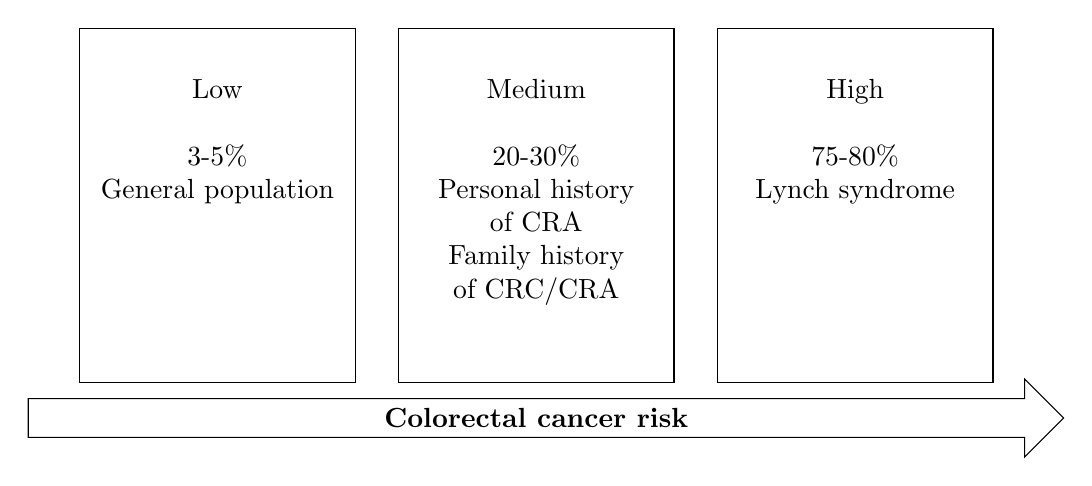
\begin{tikzpicture}[ ] 
%Declaration of styles 
\tikzstyle{box} = [rectangle, minimum width=3.5cm, minimum height=4.5cm, text centered, draw=black, text width = 3.2cm] %style for the boxes 
\tikzstyle{arr} = [single arrow, draw=black, text centered, minimum height = 13.15cm] %Style for the arrow 
 
%Nodes, the elements of the graphic 
\node [box] at (-4.05,0) {Low \quad\\ \quad\\ 3-5\% \quad\\ General population \quad\\ \quad\\ \quad\\ \quad\\ \quad\\}; 
\node [box] at (0,0) {Medium \quad\\ \quad\\  20-30\% \quad\\ Personal history \\ of CRA\\ Family history of CRC/CRA \quad\\ \quad\\}; 
\node [box] at (4.05,0) {High \quad\\ \quad\\  75-80\% \\ Lynch syndrome \quad\\ \quad\\ \quad\\ \quad\\ \quad\\}; 
\node [arr] at (0,-2.7) {\textbf{Colorectal cancer risk}}; 
\end{tikzpicture} 
\caption{Colorectal cancer risk along a continuum of clinical and genetic factors \\ Abbreviations: CRA: colorectal adenomas; CRC: colorectal cancer.} 
\label{figure1_1} 
\end{figure} 
 
\noindent In addition to the cancer-related genes and a personal/family history of colorectal adenomas and carcinomas that predispose to an increased risk of colorectal cancer, dietary and lifestyle factors are also important in influencing the risk of developing colorectal cancer, possibly in combination with genetic susceptibility to these exposures due to specific variants in related metabolising genes \cite{c126,c127}. 
 
\section{Diet and colorectal cancer} %level 1 
\noindent The 2007 Second Expert Report by the World Cancer Research Fund/American Institute for Cancer Research (WCRF/AICR) estimates that roughly one-third, and even up to one-half in some countries, of all colorectal cancers could be prevented by regular physical activity, an avoidance of body fatness within the normal range of body weight, and proper food and nutrition \cite{c126}. More specifically, as part of the WCRF/AICR Continuous Update Project (CUP), the Colorectal Cancer 2011 Report judges that with respect to diet, there is convincing evidence that foods containing dietary fibre decrease risk of colorectal cancer, while red meat, processed meat, and alcoholic drinks (particularly in men) increase risk of developing colorectal cancer \cite{c127}. There is also suggestive evidence that non-starchy vegetables, fruits, and foods containing vitamin D could lower risk of colorectal cancer \cite{c127}. Micronutrients such as folate and other B vitamins may also impact risk of developing colorectal 
cancer \cite{c126,c127}. 
 
\noindent Folate is a water-soluble B vitamin found naturally in foods that include green leafy vegetables, fruits, nuts, dairy products, potatoes and other tubers, and meat products, particularly liver \cite{c128,c129}. In contrast to naturally occurring food folate, folic acid is the synthetic, chemically-stable form of folate and is used for food fortification and in dietary supplements \cite{c130}. Other related B vitamins include riboflavin (vitamin B2), pyridoxine (vitamin B6), and cobalamin (vitamin B12). In the Netherlands, the best food sources of vitamin B2 are milk and dairy products, while vitamin B6-rich foods include meat, fish, poultry, organ meats, nuts, and lentils; eggs, dairy products, and meat are excellent sources of vitamin B12 \cite{c129}. While not a B vitamin, the essential amino acid methionine is often included along with B vitamins in explorations between these nutrients and colorectal cancer risk. The reason behind this stems from the involvement of B vitamins and methionine in 
many biological reactions in one-carbon metabolism (OCM) that when disturbed, impact colorectal carcinogenesis \cite{c131,c132}. One-carbon metabolism will be more thoroughly discussed in later in this chapter in paragraph 2 of the section titled ``B vitamins, methionine, and DNA methylation''. Good dietary sources of methionine are animal products such as meat, eggs, and dairy. 
 
\noindent As noted above in paragraph 3, variants in metabolising genes such as those involved in one-carbon metabolism, may modify the relationships between dietary and lifestyle factors and risk of colorectal cancer. The enzyme methylenetetrahydrofolate reductase (MTHFR) plays a key role in OCM because its substrate, 5,10-mTHF, mediates one-carbon groups for pyrimidine synthesis, and its product supplies one-carbon groups for methylation of DNA and other molecules. The common C to T transition in the \textit{MTHFR} gene at nucleotide 677 results in an alanine to valine substitution, subsequently producing a thermolabile variant and reduced enzyme activity \cite{c133}. This functional SNP is possibly the most well-studied of all SNPs in OCM-related genes. Results from several meta-analyses indicate that by itself, the \textit{MTHFR} 677TT genotype has not been associated with risk of developing colorectal adenomas \cite{c134,c135} but has been associated with a decreased risk of colorectal cancer compared 
with the \textit{MTHFR} 677CC genotype \cite{c134,c136}. In Lynch syndrome, the CT or TT genotype was associated with developing colorectal cancer at a later age (average age approximately 43 years) compared to those with the CC genotype (average age approximately 38 years) \cite{c137,c138}. 
 
\noindent While the \textit{MTHFR} 677TT genotype may not be associated with developing colorectal adenomas, it has been known to modify the associations between B vitamins and colorectal adenoma risk. Specifically, there has been a reduction in risk of colorectal adenomas for those with high folate intake and the TT genotype \cite{c139,c141}; low folate intake in persons with the TT genotype has been associated with an increased risk of colorectal adenomas compared with CC individuals with high folate intake \cite{c141}. Likewise, the greatest risk reduction in colorectal cancer afforded by the \textit{MTHFR} 677TT genotype is for those with high blood folate or folate intake compared to CC or CT individuals with low folate \cite{c142,c145}. In some instances, low plasma folate in TT individuals increases the risk of developing colorectal cancer compared to those with high plasma folate and the CC or CT genotype \cite{c144}. 
 
\noindent The relationships between B vitamins and methionine with colorectal cancer are enormously complex. Not only are they are further complicated by genetic variation in OCM-associated metabolising genes but also by possible synergistic influences between the B vitamins with other nutrients in our diet and in combination with different food groups and may impact colorectal carcinogenesis differently depending on the timing of exposure (i.e. from healthy tissue to adenoma to carcinoma). 
 
\subsection{B vitamins, methionine, and colorectal carcinogenesis: evidence from epidemiological studies} % level 2 
 
\subsubsection{B-vitamins, methionine, and colorectal adenoma incidence and recurrence} % level 3 
\noindent The WCRF/AICR overview of data describing associations between colorectal adenomas and food, nutrition, and physical activity was published in 2006 \cite{c146}. Using data from two cohort studies, a meta-analysis of highest versus lowest category of dietary folate intake and incidence of colorectal adenomas found a non-significant inverse association between dietary folate intake and colorectal adenoma incidence (overall relative risk (RR) (95\%CI) of 0.85 (0.66-1.11)) \cite{c146}. Total folate intake (from diet and supplements) was inversely associated with colorectal adenomas risk (overall RR (95\%CI) of 0.75 (0.56-0.99)) \cite{c146}. 
 
\noindent For those who have been diagnosed with at least one colorectal adenoma, a meta-analysis of prospective cohort studies on dietary folate intake and colorectal adenoma recurrence showed a non-significant inverse association (overall RR (95\%CI) of 0.83 (0.60-1.14) \cite{c146}. Likewise, total folate intake was non-significantly inversely associated with colorectal adenoma recurrence (overall RR (95\%CI) of 0.78 (0.48-1.29)) \cite{c146}. Also increasing plasma folate concentrations decreased risk of adenoma recurrence (OR of 0.66 (95\%CI 0.46-0.97); P-trend=0.04) for high plasma folate \textit{vs}. low plasma folate) in a prospective cohort study \cite{c147}. Five randomised controlled trials have compared the recurrence of adenomas in patients receiving folic acid supplementation daily to those receiving placebo \cite{c148,c152}. Two of the trials observed a benefit of folic acid supplementation \cite{c149,c151}, while two other trials found no effect \cite{c150,c152}. A large trial found a higher 
risk of having 3 or more adenomas or more advanced lesions ($\geq$ 25\% villous features, high-grade dysplasia, size $\geq$ 1 cm, or invasive cancer) with folic acid supplementation compared with placebo \cite{c148}. 
 
\noindent In individuals with no history of colorectal adenomas, two studies on vitamin B2 intake did not find an association with colorectal adenoma risk \cite{c153,c154}. One study did not find an association between plasma vitamin B2 and colorectal adenoma risk \cite{c155}. An inverse association between vitamin B2 intake and colorectal adenoma risk was observed in two studies \cite{c156,c157}, but only in one of these studies was the association significant \cite{c156}. Vitamin B6 intake is often \cite{c147,c153} but also not always \cite{c156} inversely associated with developing colorectal adenomas. There are also reports of inverse associations between the main circulating form of vitamin B6, PLP (pyridoxal 5'-phosphate), and colorectal adenoma risk \cite{c155,c158}. In the majority of studies, vitamin B12 status seems to be unassociated with first colorectal adenoma risk \cite{c155,c156,c158}. A meta-analysis of highest versus lowest category of methionine intake and colorectal adenoma incidence has 
been conducted using estimates from two cohort studies \cite{c146}. The pooled RR for colorectal adenoma incidence was 0.53 (0.25-1.11) \cite{c146}. In a cross-sectional study, plasma methionine was inversely associated with developing distal colorectal adenomas \cite{c155}. 
 
\noindent For those who have had at least one colorectal adenoma in their lifetime, vitamin B6 intake was inversely associated with risk of adenoma recurrence (OR of 0.65 (95\%CI 0.45-0.94); P-trend=0.03 for the highest quartile of intake \textit{vs}. the lowest) \cite{c147}. Likewise, vitamin B12 intake was inversely associated with risk of adenoma recurrence in a patients who had previously participated in an intervention study with wheat bran, but this association did not reach significance (for the highest quartile of intake \textit{vs}. lowest quartile OR of 0.74 (95\%CI 0.51-1.08); P-trend=0.14) \cite{c147}. One cohort study has reported an inverse but not significant association between methionine intake and recurrence of colorectal adenomas \cite{c147}. We are unaware of any studies on vitamin B2 intake and colorectal adenoma recurrence. Overall, foods containing folate, other B vitamins, and methionine may offer some protection against developing first or recurrent colorectal adenomas, but studies 
are not entirely consistent, particularly for vitamin B2, vitamin B12, and methionine, where the evidence is also more sparse. 
 
\subsubsection{B-vitamins, methionine, and colorectal cancer incidence} % level 3 
\noindent The earliest documented epidemiological observation of a link between folate intake and colorectal cancer was published in 1989 \cite{c159}. Decades of epidemiological research on folate, and more generally diet, and colorectal cancer have since followed. In 2005, Sanjoaquin and colleagues performed a meta-analysis of 7 cohort studies on folate intake and colorectal cancer risk and found an inverse association between dietary folate intake and colorectal cancer (overall RR for high \textit{vs}. low intake = 0.75; 95\%CI=0.64-0.89) \cite{c160}. These results have been corroborated by two meta-analyses \cite{c126,c161}, one of which was from the Second Expert Report (SER) by the WCRF/AICR that gave a summary effect estimate for the association between dietary folate intake and colorectal cancer of 0.84 (95\%CI 0.76-0.93) per 100 $\mu$g dietary folate/day \cite{c126}. Likewise, the most recent WCRF/AICR CUP summary estimates from meta-analyses for dietary folate intake and risk of colorectal cancer 
were also in the direction of decreased risk with increasing folate intake but did not reach statistical significance (summary effect estimate of 0.99 (95\%CI 0.93-1.05)) \cite{c127}. 
 
\noindent CUP summary relative risks from meta-analyses for serum/plasma folate (per 2 ng/mL) were also in the direction of decreased risk for colorectal cancer, colon cancer, and rectal cancer with increasing serum/plasma folate concentrations but were not significant (summary estimate of 0.97 (95\%CI 0.93-1.00) for colorectal cancer, 0.98 (0.85-1.14) for colon cancer, and 0.87 (0.70-1.09) for rectal cancer) \cite{c127}. Results from a pooled analysis of 5,720 colon cancer cases among 725,134 participants from 13 cohort studies showed a borderline significant decreased risk for those in the highest quintile of dietary folate intake compared with lowest group (pooled multivariate RR (95\%CI) of 0.92 (0.84-1.00)) \cite{c162}. Based on the current evidence, the WCRF/AICR has concluded that the evidence is too limited to draw conclusions about foods containing folate and risk of colorectal cancer. 
 
\noindent Regarding folic acid supplementation trials, a meta-analysis of randomised controlled trials has found no effect of folic acid supplementation on incidence of colorectal cancer \cite{c163}. Based on these results, folate may contribute a small protective effect against colorectal cancer, but because there are several inconsistencies results should be interpreted with prudence. 
 
\noindent Concerning the other B vitamins, there have been suggestions that higher vitamin B2 intakes \cite{c164} and higher concentrations of vitamin B2 in plasma/serum \cite{cc165,c166} are associated with decreased risk of colorectal cancer, but to the best of our knowledge, no meta-analyses have been published thus far. For vitamin B6, the results of a meta-analysis that included nine prospective studies on vitamin B6 intake and four studies on PLP concentrations showed inverse associations between colorectal cancer risk and vitamin B6 intake (overall RR of 0.90 (0.75-1.07) for the highest \textit{vs} lowest category) and PLP concentrations (overall RR of  0.52 (95\% CI, 0.38-0.71 for the highest \textit{vs} lowest category) \cite{c167}. The relationships between vitamin B12 intake or plasma/serum vitamin B12 and colorectal cancer are less clear with most studies observing null associations \cite{c166,c168,c169,c170}. One study found an inverse association between methionine intake and colorectal cancer 
risk \cite{c164} while no associations were observed in two studies \cite{c168,c170}. Overall, these results taken together emphasise the need for more unambiguous evidence that describe associations between B vitamins and colorectal carcinogenesis. 
 
\section{Colorectal carcinogenesis: a continuum of genetic and epigenetic changes} % level 1 
Like all cancers, those that develop in the colon and rectum result from unregulated cellular growth. Over time, a stepwise accumulation of significant alterations, brought on by intrinsic or environmental factors \textendash~or a combination of both \textendash~modify the normal regulatory functions and dynamics of a cell \cite{c126}. As mentioned in paragraph 1 of this introduction, most precursor lesions of colorectal carcinomas are colorectal adenomas, and evolution from adenomas to carcinomas is termed the \textit{adenoma-carcinoma sequence} \cite{c14,c17}, during which tissues in the colon and rectum undergo histopathological changes with tissues becoming increasingly dysplastic \cite{c171}. The transition from normal epithelium to adenoma to carcinoma is accompanied by acquired molecular events that include genetic and epigenetic alterations \cite{c14,c172,c173}. 
 
\subsection{Genetic alterations during colorectal carcinogenesis} % level 2 
One of the earliest events of sporadic colorectal cancer progression that is required for colorectal adenoma formation is somatic bi-allelic inactivation of the tumour suppressor gene adenomatous polyposis coli (\textit{APC}) gene, leading to activation of the Wnt signalling pathway \cite{c174}. As well, Wnt signalling in some cancers may be activated by mutations in $\beta$-catenin. Wnt activation induces genes that include c-\textit{myc}, \textit{cyclin D1}, and \textit{PPAR-$\delta$} \cite{c175}. Transformation from early to late adenomas to carcinomas are likely due to mutations and/or loss of heterozygosity in the oncogene Kirsten-ras (\textit{KRAS}) \cite{c176}; mutations in the tumour suppressor gene \textit{p53} are proposed to be later events in the development of colorectal carcinomas \cite{c177}. The genetic basis of Lynch syndrome has been discussed in paragraph 2 of this chapter. Genetic changes in a cell during colorectal cancer progression are often accompanied by and interact with epigenetic 
modifications. 
 
\subsection{Epigenetic alterations during colorectal carcinogenesis} % level 2 
Epigenetics was first defined by C.H. Waddington as ``the causal interactions between genes and their products, which bring the phenotype into being'' \cite{c178}; the definition of epigenetics now encompasses the heritable changes in gene expression that occur independent of alterations in the DNA sequence \cite{c179}. Epigenetic processes include posttranslational modifications of histone proteins, nucleosome positioning along the DNA, and possibly the best-known of these processes, DNA methylation \cite{c173,c180}. 
 
\subsubsection{DNA methylation} % level 3 
DNA methylation occurs at the C-5 position of cytosine residues located in the CpG dinucleotide called CpG sites \cite{c181}. CpG sites, while under-represented in the genome, are found clustered together in C- and G-rich regions termed CpG islands, usually in the promoters or gene-regulating regions of genes. The remaining CpG sites are interspersed throughout the genome in transposable elements, repetitive sequences or other intronic regions of DNA. Typically in a healthy cell, most CpG islands are unmethylated and the associated genes subsequently expressed, while CpG sites are methylated \cite{c182,c183}. The methylation of CpG sites probably works to prevent chromosomal instability, translocations, and gene disruption caused by reactivation of transposable DNA sequences \cite{c184}. There are generally two different types of DNA methylation that can be described \textendash~gene-specific and global. 
 
\paragraph{Gene-specific DNA methylation} % level 4 
CpG islands in gene promoters or gene-regulating regions of genes are normally unmethylated in order to allow transcription of their corresponding genes. In cancer, these CpG islands may become more methylated (called gene-specific or promoter hypermethylation), which results in transcriptional silencing \cite{c185}. CpG island hypermethylation of promoters can affect genes involved in cell cycle, DNA repair, carcinogen metabolism, cell-cell interaction, apoptosis, and angiogenesis, all of which are related to carcinogenesis \cite{c182}. In colorectal carcinogenesis, CpG island promoter hypermethylation has been known to inactivate genes such as \textit{MLH1} (mismatch repair), \textit{p16\textsuperscript{INK4a}} (tumour suppressor), \textit{p14\textsuperscript{ARF}} (tumour suppressor), \textit{MGMT} (DNA repair), and \textit{RASSF1A} (tumour suppressor) \cite{c186,c187} in addition to numerous others. 
 
\paragraph{Global DNA methylation} % level 4 
In cancer, CpG sites that are distributed among the genome become less methylated, a process which is called global hypomethylation. Global hypomethylation is an early event in colorectal carcinogenesis \cite{c188,c189}. More explicitly, Fearon and Vogelstein's Genetic Model for Colorectal Tumorigenesis describes global DNA hypomethylation as an earlier event along the \textit{adenoma-carcinoma sequence} with gene-specific DNA methylation occurring later \cite{c14}. Because global DNA methylation is an earlier event in colorectal carcinogenesis and the aim of this thesis is to investigate relationships between B vitamins and DNA methylation along a continuum of risk for colorectal cancer that includes low-risk individuals, this thesis will focus on global DNA methylation. 
 
\paragraph{Measuring global DNA methylation in epidemiological studies} % level 4 
A plethora of methods have been developed to measure global DNA methylation, although the ``best'' method will depend on the number of samples, quality and quantity of available DNA, and desired coverage and resolution \cite{c190}. Chromatographic methods for measuring global DNA methylation allow for direct quantification of methylation. Following digestion of DNA into single strands, chromatographic methods directly measure the total number of 5 methyl cytosines and cytosines. Chromatography allows for direct quantification of DNA methylation but is time-consuming, costly and highly specialised equipment as well as large amounts of DNA are required, which can be cumbersome for large epidemiological studies \cite{c191}. As a possible alternative, in 2004, Yang and colleagues developed a PCR-based method to evaluate global DNA methylation by semi-quantitatively measuring methylation of long interspersed nuclear elements (LINEs) using bisulfite pyrosequencing \cite{c146}. LINEs are a variety of transposable 
elements. Transposable elements are mobile sequences of repetitive DNA that can migrate to different regions of the genome. There are two related LINE families, but the majority of genomic DNA is comprised of LINE-1 (18\%) \cite{c147}. Methylation of repetitive DNA elements such as LINE-1 is frequently used as a surrogate for global DNA methylation in epidemiological studies, including those where B vitamins are investigated as possible determinants of global DNA methylation \cite{c148,c151}. 
 
\section{B vitamins, methionine, and DNA methylation} % level 1 
As mentioned in paragraph 5, several B vitamins including folate play an essential role in one-carbon metabolism (OCM), where perturbations of B vitamins and methionine may have an effect on DNA methylation. One-carbon metabolism is a complex network of interconnected reactions involving a multitude of substrates, enzymes and cofactors \cite{c192} (see Figure \ref{focm}). Folate is a carrier of one-carbon units in OCM, where it plays a central role in DNA methylation, nucleotide synthesis, and maintaining DNA stability and repair \cite{c132,c193,c194,c195,c196}. 
 
\noindent In addition to folate, the B vitamins riboflavin (vitamin B2), pyridoxine (vitamin B6), and cobalamin (vitamin B12), and the essential amino acid methionine are also important in supporting efficient one-carbon metabolism \cite{c197}. Riboflavin in its coenzymatic form of flavin adenine dinucleotide (FAD) is essential for the enzyme methylenetetrahydrofolate reductase (MTHFR) in the irreversible reduction of 5,10-methylenetetrahydrofolate (5,10-methylene-THF) to 5-methyl-THF (5-mTHF) \cite{c198}. Vitamin B6 as pyridoxal 5'\ -phosphate is a coenzyme for serine hydroxymethyltransferase (SHMT) in the reversible conversion of tetrahydrofolate (THF) to 5,10-methylene-THF \cite{c199} while the remethylation of homocysteine to methionine by methionine synthase (MTR) and methionine synthase reductase (MTRR) with 5-methyl-THF as a methyl donor is dependent on cobalamin \cite{c1100,c1101}. Methionine is consequently metabolised to \textit{S}-adenosylmethionine (SAM), the universal methyl donor for over one 
hundred biological reactions including DNA methylation \cite{c1102}. High concentrations of homocysteine in blood are related to low blood concentrations of folate \cite{c1103}. Although B vitamins and methionine are involved in DNA synthesis and DNA stability and repair, which also influence colorectal cancer, this thesis focuses on the involvement of B vitamins on global DNA methylation. 
 
% FIGURE 2 HERE 
\begin{figure} 
\centering 
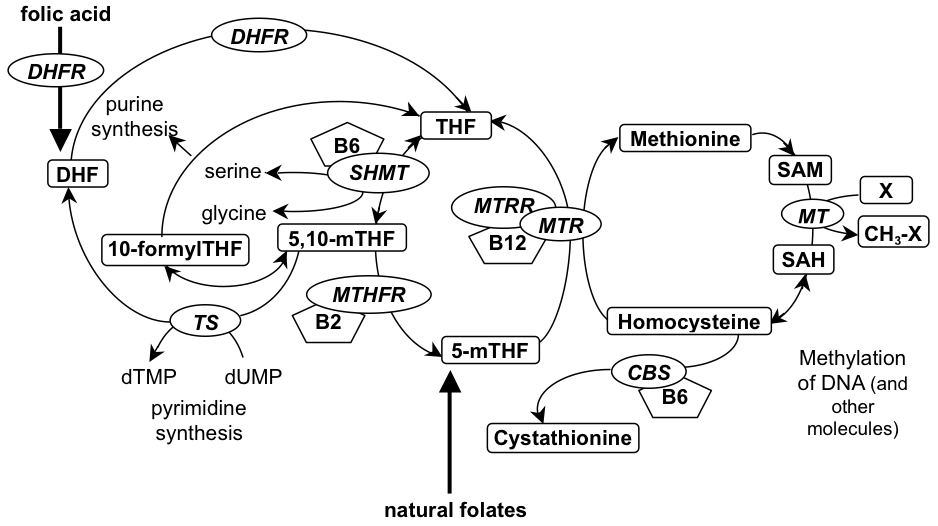
\includegraphics[width=0.85\textwidth]{ocm_xls5.jpg} 
\caption{Folate-mediated one-carbon metabolism. Abbreviations: DHF: dihydrofolate; DHFR: dihydrofolate reductase; THF: tetrahydrofolate; SHMT: serine hydroxymethyltransferase; 10-formylTHF: 10-formyltetrahydrofolate; 5,10-mTHF: 5,10-methylenetetrahydrofolate; 5-mTHF: 5-methyltetrahydrofolate; MTHFR: methylenetetrahydrofolate reductase; MTRR: methionine synthase reductase; MTR: methionine synthase; CBS: cystathionine $\beta$-synthase; MT: methyltransferase; SAM: \emph{S}-adenosylmethionine; SAH: \emph{S}-adenosylhomocysteine} 
\label{focm} 
\end{figure} 
 
 
\section{B vitamins and leukocyte DNA methylation: \\ evidence from epidemiological studies} % level 1 
The role of B vitamins along the continuum of colorectal carcinogenesis is not straightforward, and may depend on a plethora of factors, such as inefficient OCM, personal history of colorectal adenomas, a family history of colorectal adenomas and carcinomas, and inherited mutations in cancer-associated genes. Likewise, the impact of B vitamins on DNA methylation could be moderated by the presence or absence of these factors. 
 
\noindent The relationships between B vitamins and DNA methylation have been studied in normal colorectal tissues \cite{c1104,c1105}, colorectal adenomas \cite{c1106}, and colorectal carcinomas \cite{c1107,c1108}. With this in mind, the intent of this thesis is to better understand the influence of B vitamins on leukocyte global DNA methylation of populations differing in risk for colorectal cancer. 
 
\subsection{Low risk population} % level 2 
There have been two relatively short-term (12 weeks) randomised placebo-controlled trials investigating the effects of folic acid supplementation on leukocyte global DNA methylation in populations at low-risk for colorectal cancer \cite{c1109,c1110}. At the end of 12 weeks, neither trial found an effect of 1.2 mg \cite{c1109} nor 2 mg \cite{c1110} daily folic acid supplementation on global DNA methylation. A possible explanation for these null results could be the short duration of folic acid supplementation and the use of supraphysiological doses of folic acid. Two cross-sectional studies, one in urban commuters in the United States and the other in older Brazilians (aged 60-88 years) have reported that neither intake of natural folates nor dietary folate equivalents was associated with leukocyte LINE-1 methylation \cite{c1111}, nor global DNA methylation \cite{c1112}. A third cross-sectional study observed that higher dietary folate intake was associated with lower global DNA methylation in Japanese women \
cite{c1113}. Geographical differences, food fortification, different dietary habits, and baseline folate concentrations are some reasons that could possibly account for these dissimilar results. Similarly, plasma folate has been unassociated with leukocyte global methylation in a cross-sectional analysis \cite{c1114} in contrast to two other controlled folate intake studies in women, where leukocyte global DNA methylation decreased following folate depletion \cite{c1115,c1116}. In one of these studies, DNA hypomethylation was reversed following folate repletion \cite{c1115}, but not in the other \cite{c1116}. This is likely due to the study population, comprised exclusively of elderly women, where stabilisation of DNA methylation following folate depletion could be delayed, resulting also in a slower response to folate repletion. 

\noindent Three cross-sectional studies have examined relationships between intake of other B vitamins and leukocyte DNA methylation \cite{c1111,c1113}. One study found a weak negative correlation between vitamin B6 intake and global DNA methylation (Spearman $\rho$ of -0.18, P=0.04) \cite{c1112}. Vitamin B12 intake was not related to global DNA methylation, and vitamin B2 was not investigated \cite{c1112}. On the other hand, intake of vitamins B2, B6, and B12 were not associated with leukocyte global DNA methylation in an urban American population \cite{c1111}, nor in Japanese women \cite{c1113}. 
 
\subsection{High risk population} % level 2 
The association between B vitamins and global DNA methylation has been investigated in colorectal adenoma patients. These associations have not yet been explored in a Lynch syndrome population. In colorectal adenoma patients, the effects of folic acid supplementation on global DNA methylation were investigated \cite{c1117}. After 10 weeks of daily supplementation with 400 $\mu$g folic acid, leukocyte global DNA methylation increased 31\% (95\%CI 16-47\%; p=0.05 \textit{vs}. placebo). Here, the dose and duration of folic acid supplementation was lower and shorter, respectively than in trials with low-risk participants, but there was an effect on global DNA methylation, which was measured using the same method as in the other low-risk trials. Baseline red blood folate also appeared to be similar between the three populations. Drawing firm conclusions is not possible based on one study, but it is possible to speculate that folic acid has a different effect on DNA methylation depending on which phase during 
carcinogenesis it is given. Additionally, genetic variation in OCM-related genes, such \textit{MTHFR}, could modify the relationships between B vitamins and methionine with DNA methylation. 
 
\section{B vitamins and DNA methylation: interactions with \emph{MTHFR} C677T} % level 1 
Main effects of the \textit{MTHFR} C677T genotype on global DNA methylation have been explored in several studies. In low risk populations, there has been no difference in leukocyte global DNA methylation levels between genotypes \cite{c1112,c1114}. However, the C677T polymorphism in this gene may modify associations between plasma folate and global DNA methylation and LINE-1 DNA methylation. 
 
\subsection{Low risk population} % level 2 
Two studies have suggested that leukocyte DNA is hypomethylated in persons with low folate status and homozygous for the TT genotype \cite{c133,c1118|}. In a folate depletion-repletion study, women with the TT genotype had a greater in increase in leukocyte DNA global DNA methylation following folate repletion compared with the CC genotype \cite{c1119}. A similar folate depletion-repletion study found lower levels of leukocyte DNA methylation in women with the TT genotype following repletion compared with CC or CT women \cite{c1120}. The slow response in DNA methylation levels to folate repletion has been partly attributed to a slow turnover of whole-body folate pools \cite{c1121}. On the whole, there seem to be interactions between folate intake and \textit{MTHFR} C677T in a low-risk population. The largest variation in global DNA methylation (i.e. greatest increase and decrease of global DNA methylation) by folate intake appear to be most clear in those with the \textit{MTHFR} 677TT genotype. 
 
\subsection*{High risk population} % level 2 
In very high risk populations, data on B vitamin-colorectal cancer relationships are not yet available. There was no information about dietary information nor DNA methylation from the two studies that investigated the main effects of the \textit{MTHFR} C677T single nucleotide polymorphism on colorectal cancer risk in persons with Lynch syndrome \cite{c137,c138}. 
 
\section{Rationale and Outline of this Thesis} % level 1 
The main purpose of the studies presented in this thesis is to improve our knowledge about the associations between B vitamin and methionine status and leukocyte global DNA methylation in populations with differential risk for developing colorectal cancer. Figure \ref{figure3} is an illustration of the clinical, genetic, and nutritional factors that influence differential risk for colorectal cancer along a continuum as outlined in this thesis according to each chapter. Given that DNA methylation is one of the major mechanisms linking B vitamins and other nutritional factors to colorectal cancer, \textbf{Chapter 2} is a review that summarises the impact of nutrition on DNA methylation in different cancer sites as explored in epidemiological studies. 
 
\noindent In order to study the relationships between B vitamin status and global DNA methylation in different risk groups, we use data from four study populations differing in colorectal cancer risk, as shown in Figure \ref{figure3}. Contributions from these studies begin in \textbf{Chapter 3} where the relationship between plasma folate and leukocyte LINE-1 methylation in a low risk population was explored. A study detailing the effects of folic acid supplementation on leukocyte global DNA methylation in individuals with moderately elevated homocysteine is presented in \textbf{Chapter 4}. Moving further along the risk scale for colorectal cancer, \textbf{Chapter 5} investigates the associations between plasma B vitamins and methionine, and LINE-1 methylation in colorectal adenoma patients; additional effect modification by number of lifetime colorectal adenomas was also explored. Associations between dietary B vitamin and methionine intake and risk of colorectal tumours in Lynch Syndrome individuals are 
studied in \textbf{Chapter 6}. This thesis concludes (\textbf{Chapter 7}) with a discussion of the results from all our studies. Recommendations for future research and public health implications are additionally considered. 
 
% FIGURE 3 HERE 
\begin{figure} 
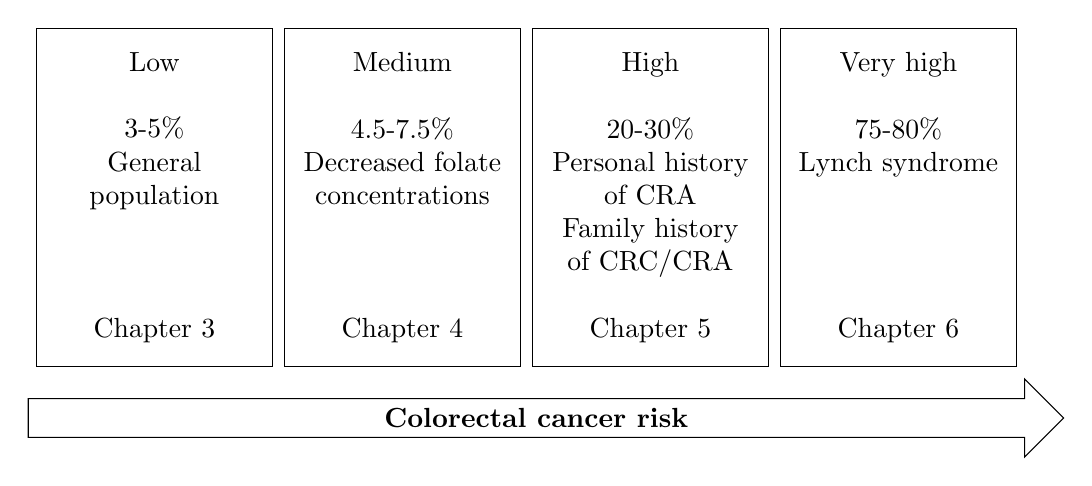
\begin{tikzpicture}[ ] 
%Declaration of styles 
	\tikzstyle{box} = [rectangle, minimum width=3.0cm, minimum height=4.3cm, text centered, draw=black, text width = 2.7cm] %style for the boxes 
	\tikzstyle{arr} = [single arrow, draw=black, text centered, minimum height = 13.15cm] %Style for the arrow 
%Nodes, the elements of the graphic 
	\node [box] at (-4.85,0) {Low \quad\\ \quad\\ 3-5\% \quad\\ General population \quad\\ \quad\\ \quad\\ \quad\\Chapter 3}; 
	\node [box] at (-1.70,0) {Medium \quad\\ \quad\\ 4.5-7.5\%\quad\\ Decreased folate\\concentrations \quad\\ \quad\\ \quad\\ \quad\\Chapter 4}; 
    	\node [box] at (1.45,0) {High \quad\\ \quad\\ 20-30\% \\ Personal history \\ of CRA \\ Family history of CRC/CRA \quad\\ \quad\\Chapter 5}; 
    	\node [box] at (4.60,0) {Very high \quad\\ \quad\\ 75-80\% \quad\\ Lynch syndrome \quad\\ \quad\\ \quad\\ \quad\\ \quad\\Chapter 6}; 
    	\node [arr] at (0,-2.8) {\textbf{Colorectal cancer risk}}; 
\end{tikzpicture} 
\caption{Colorectal cancer risk along a continuum of clinical, genetic, and nutritional factors according to the chapters of this thesis.} 
\label{figure3} 
\end{figure} 
 
 
\renewcommand{\bibname}{References} 
\begin{thebibliography}{12} 
	\bibitem{c11}	Ferlay J, Shin HR, Bray F, Forman D, Mathers C, Parkin DM. GLOBOCAN 2008 v2.0, Cancer Incidence and Mortality Worldwide: IARC CancerBase No. 10 [Internet]. Lyon, France: International Agency for Research on Cancer; 2010. Available from: http://globocan.iarc.fr, accessed on 21/08/2013. 
	\bibitem{c12}	Siegel R, Naishadham D, Jemal A. Cancer statistics, 2013. CA: a cancer journal for clinicians. 2013 Jan;63(1):11-30. 
	\bibitem{c13}	Butterworth AS, Higgins JP, Pharoah P. Relative and absolute risk of colorectal cancer for individuals with a family history: a meta-analysis. Eur J Cancer. 2006 Jan;42(2):216-27. 
	\bibitem{c14}	Fearon ER, Vogelstein B. A genetic model for colorectal tumorigenesis. Cell. 1990 Jun 1;61(5):759-67. 
	\bibitem{c15}	Morson BC. Precancerous lesions of the colon and rectum. Classification and controversial issues. JAMA. 1962 Feb 3;179:316-21. 
	\bibitem{c16}	Chen CD, Yen MF, Wang WM, Wong JM, Chen TH. A case-cohort study for the disease natural history of adenoma-carcinoma and de novo carcinoma and surveillance of colon and rectum after polypectomy: implication for efficacy of colonoscopy. British Journal of Cancer. 2003 Jun 16;88(12):1866-73. 
	\bibitem{c17}	Hill MJ, Morson BC, Bussey HJ. Aetiology of adenoma--carcinoma sequence in large bowel. Lancet. 1978 Feb 4;1(8058):245-7. 
	\bibitem{c18}	Loeve F, van Ballegooijen M, Boer R, Kuipers EJ, Habbema JD. Colorectal cancer risk in adenoma patients: a nation-wide study. International Journal of Cancer. 2004 Aug 10;111(1):147-51. 
	\bibitem{c19}	Simons BD, Morrison AS, Lev R, Verhoek-Oftedahl W. Relationship of polyps to cancer of the large intestine. Journal of the National Cancer Institute. 1992 Jun 17;84(12):962-6. 
	\bibitem{c110}	Atkin WS, Morson BC, Cuzick J. Long-term risk of colorectal cancer after excision of rectosigmoid adenomas. The New England Journal of Medicine. 1992 Mar 5;326(10):658-62. 
	\bibitem{c111}	de la Chapelle A. The incidence of Lynch syndrome. Familial cancer. 2005;4(3):233-7. 
	\bibitem{c112}	Aarnio M, Mecklin JP, Aaltonen LA, Nystrom-Lahti M, Jarvinen HJ. Life-time risk of different cancers in hereditary non-polyposis colorectal cancer (HNPCC) syndrome. International Journal of Cancer. 1995 Dec 20;64(6):430-3. 
	\bibitem{c113}	Aarnio M, Sankila R, Pukkala E, Salovaara R, Aaltonen LA, de la Chapelle A, et al. Cancer risk in mutation carriers of DNA-mismatch-repair genes. International Journal of Cancer. 1999 Apr 12;81(2):214-8. 
	\bibitem{c114}	Weitz J, Koch M, Debus J, Hohler T, Galle PR, Buchler MW. Colorectal cancer. Lancet. 2005 Jan 8-14;365(9454):153-65. 
	\bibitem{c115}	Dunlop MG, Farrington SM, Carothers AD, Wyllie AH, Sharp L, Burn J, et al. Cancer risk associated with germline DNA mismatch repair gene mutations. Human molecular genetics. 1997 Jan;6(1):105-10. 
	\bibitem{c116}	Watson P, Lynch HT. Cancer risk in mismatch repair gene mutation carriers. Familial cancer. 2001;1(1):57-60. 
	\bibitem{c117}	Vasen HF, Wijnen JT, Menko FH, Kleibeuker JH, Taal BG, Griffioen G, et al. Cancer risk in families with hereditary nonpolyposis colorectal cancer diagnosed by mutation analysis. Gastroenterology. 1996 Apr;110(4):1020-7. 
	\bibitem{c118}	Vasen HF, Moslein G, Alonso A, Bernstein I, Bertario L, Blanco I, et al. Guidelines for the clinical management of Lynch syndrome (hereditary non-polyposis cancer). Journal of Medical Genetics. 2007 Jun;44(6):353-62. 
	\bibitem{c119}	Richard GF, Kerrest A, Dujon B. Comparative genomics and molecular dynamics of DNA repeats in eukaryotes. Microbiol Mol Biol Rev. 2008 Dec;72(4):686-727. 
	\bibitem{c120}	Koole W, Schafer HS, Agami R, van Haaften G, Tijsterman M. A versatile microsatellite instability reporter system in human cells. Nucleic acids research. 2013 Jul 16. 
	\bibitem{c121}	Lynch HT, de la Chapelle A. Hereditary colorectal cancer. The New England Journal of Medicine. 2003 Mar 6;348(10):919-32. 
	\bibitem{c122}	Half EE, Bresalier RS. Clinical management of hereditary colorectal cancer syndromes. Current opinion in gastroenterology. 2004 Jan;20(1):32-42. 
	\bibitem{c123}	Hampel H, Stephens JA, Pukkala E, Sankila R, Aaltonen LA, Mecklin JP, et al. Cancer risk in hereditary nonpolyposis colorectal cancer syndrome: later age of onset. Gastroenterology. 2005 Aug;129(2):415-21. 
	\bibitem{c124}	Watson P, Lynch HT. The tumor spectrum in HNPCC. Anticancer Research. 1994 Jul-Aug;14(4B):1635-9. 
	\bibitem{c125}	Kastrinos F, Mukherjee B, Tayob N, Wang F, Sparr J, Raymond VM, et al. Risk of pancreatic cancer in families with Lynch syndrome. JAMA. 2009 Oct 28;302(16):1790-5. 
	\bibitem{c126}	World Cancer Research Fund/American Institute for Cancer Research. Food, Nutrition, Physical Activity, and the Prevention of Cancer: a Global Perspective. Washington DC: AICR, 2007. 
	\bibitem{c127}	World Cancer Research Fund/American Institute for Cancer Research. Continuous Update Project Report. Food, Nutrition, Physical Activity, and the Prevention of Colorectal Cancer. 2011. 
	\bibitem{c128}	Konings EJ, Roomans HH, Dorant E, Goldbohm RA, Saris WH, van den Brandt PA. Folate intake of the Dutch population according to newly established liquid chromatography data for foods. The American Journal of Clinical Nutrition. 2001 Apr;73(4):765-76. 
	\bibitem{c129}	van Rossum CTM, Fransen HP, Verkaik-Kloosterman J, Buurma-Rethans EJM, Ock MC. Dutch National Food Consumption Survey 2007-2010. Bilthoven: National Institute for Public Health and the Environment; 2011. Report No.: 350050006/2011. 
	\bibitem{c130}	Winkels RM, Brouwer IA, Siebelink E, Katan MB, Verhoef P. Bioavailability of food folates is 80\% of that of folic acid. The American Journal of Clinical Nutrition. 2007 Feb;85(2):465-73. 
	\bibitem{c131}	Little J, Sharp L, Duthie S, Narayanan S. Colon cancer and genetic variation in folate metabolism: the clinical bottom line. The Journal of Nutrition. 2003 Nov;133(11 Suppl 1):3758S-66S. 
	\bibitem{c132}	Ulrich CM. Nutrigenetics in cancer research--folate metabolism and colorectal cancer. The Journal of Nutrition. 2005 Nov;135(11):2698-702. 
	\bibitem{c133}	Friso S, Choi SW, Girelli D, Mason JB, Dolnikowski GG, Bagley PJ, et al. A common mutation in the 5,10-methylenetetrahydrofolate reductase gene affects genomic DNA methylation through an interaction with folate status. Proceedings of the National Academy of Sciences of the United States of America. 2002 Apr 16;99(8):5606-11. 
	\bibitem{c134}	Huang Y, Han S, Li Y, Mao Y, Xie Y. Different roles of MTHFR C677T and A1298C polymorphisms in colorectal adenoma and colorectal cancer: a meta-analysis. Journal of human genetics. 2007;52(1):73-85. 
	\bibitem{c135}	Zacho J, Yazdanyar S, Bojesen SE, Tybjaerg-Hansen A, Nordestgaard BG. Hyperhomocysteinemia, methylenetetrahydrofolate reductase c.677C>T polymorphism and risk of cancer: cross-sectional and prospective studies and meta-analyses of 75,000 cases and 93,000 controls. International Journal of Cancer. 2011 Feb 1;128(3):644-52. 
	\bibitem{c136}	Taioli E, Garza MA, Ahn YO, Bishop DT, Bost J, Budai B, et al. Meta- and pooled analyses of the methylenetetrahydrofolate reductase (MTHFR) C677T polymorphism and colorectal cancer: a HuGE-GSEC review. American Journal of Epidemiology. 2009 Nov 15;170(10):1207-21. 
	\bibitem{c137}	Pande M, Chen J, Amos CI, Lynch PM, Broaddus R, Frazier ML. Influence of methylenetetrahydrofolate reductase gene polymorphisms C677T and A1298C on age-associated risk for colorectal cancer in a caucasian lynch syndrome population. Cancer Epidemiol Biomarkers Prev. 2007 Sep;16(9):1753-9. 
	\bibitem{c138}	Reeves SG, Meldrum C, Groombridge C, Spigelman AD, Suchy J, Kurzawski G, et al. MTHFR 677 C>T and 1298 A>C polymorphisms and the age of onset of colorectal cancer in hereditary nonpolyposis colorectal cancer. Eur J Hum Genet. 2009 May;17(5):629-35. 
	\bibitem{c139}	Ulvik A, Evensen ET, Lien EA, Hoff G, Vollset SE, Majak BM, et al. Smoking, folate and methylenetetrahydrofolate reductase status as interactive determinants of adenomatous and hyperplastic polyps of colorectum. American Journal of Medical Genetics. 2001 Jul 1;101(3):246-54. 
	\bibitem{c140}	Marugame T, Tsuji E, Kiyohara C, Eguchi H, Oda T, Shinchi K, et al. Relation of plasma folate and methylenetetrahydrofolate reductase C677T polymorphism to colorectal adenomas. International Journal of Epidemiology. 2003 Feb;32(1):64-6. 
	\bibitem{c141}	Ulrich CM, Kampman E, Bigler J, Schwartz SM, Chen C, Bostick R, et al. Colorectal adenomas and the C677T MTHFR polymorphism: evidence for gene-environment interaction? Cancer Epidemiol Biomarkers Prev. 1999 Aug;8(8):659-68. 
	\bibitem{c142}	Le Marchand L, Wilkens LR, Kolonel LN, Henderson BE. The MTHFR C677T polymorphism and colorectal cancer: the multiethnic cohort study. Cancer Epidemiol Biomarkers Prev. 2005 May;14(5):1198-203. 
	\bibitem{c143}	Chen J, Giovannucci E, Kelsey K, Rimm EB, Stampfer MJ, Colditz GA, et al. A methylenetetrahydrofolate reductase polymorphism and the risk of colorectal cancer. Cancer research. 1996 Nov 1;56(21):4862-4. 
	\bibitem{c144}	Ma J, Stampfer MJ, Giovannucci E, Artigas C, Hunter DJ, Fuchs C, et al. Methylenetetrahydrofolate reductase polymorphism, dietary interactions, and risk of colorectal cancer. Cancer research. 1997 Mar 15;57(6):1098-102. 
	\bibitem{c145}	Slattery ML, Potter JD, Samowitz W, Schaffer D, Leppert M. Methylenetetrahydrofolate reductase, diet, and risk of colon cancer. Cancer Epidemiol Biomarkers Prev. 1999 Jun;8(6):513-8. 
	\bibitem{c146}	The associations between food, nutrition, and physical activity and the risk of colorectal polyps and underlying mechanisms (online): World Cancer Research Fund/American Institute for Cancer Research; 2006. 
	\bibitem{c147}	Martinez ME, Henning SM, Alberts DS. Folate and colorectal neoplasia: relation between plasma and dietary markers of folate and adenoma recurrence. The American Journal of Clinical Nutrition. 2004 Apr;79(4):691-7. 
	\bibitem{c148}	Cole BF, Baron JA, Sandler RS, Haile RW, Ahnen DJ, Bresalier RS, et al. Folic acid for the prevention of colorectal adenomas: a randomized clinical trial. JAMA. 2007 Jun 6;297(21):2351-9. 
	\bibitem{c149}	Jaszewski R, Misra S, Tobi M, Ullah N, Naumoff JA, Kucuk O, et al. Folic acid supplementation inhibits recurrence of colorectal adenomas: a randomized chemoprevention trial. World J Gastroenterol. 2008 Jul 28;14(28):4492-8. 
	\bibitem{c150}	Logan RF, Grainge MJ, Shepherd VC, Armitage NC, Muir KR. Aspirin and folic acid for the prevention of recurrent colorectal adenomas. Gastroenterology. 2008 Jan;134(1):29-38. 
	\bibitem{c151}	Paspatis GA, Karamanolis DG. Folate supplementation and adenomatous colonic polyps. Diseases of the Colon and Rectum. 1994 Dec;37(12):1340-1. 
	\bibitem{c152}	Wu K, Platz EA, Willett WC, Fuchs CS, Selhub J, Rosner BA, et al. A randomized trial on folic acid supplementation and risk of recurrent colorectal adenoma. The American Journal of Clinical Nutrition. 2009 Dec;90(6):1623-31. 
	\bibitem{c153}	Benito E, Cabeza E, Moreno V, Obrador A, Bosch FX. Diet and colorectal adenomas: a case-control study in Majorca. International Journal of Cancer. 1993 Sep 9;55(2):213-9. 
	\bibitem{c154}	Macquart-Moulin G, Riboli E, Cornee J, Kaaks R, Berthezene P. Colorectal polyps and diet: a case-control study in Marseilles. International Journal of Cancer. 1987 Aug 15;40(2):179-88. 
	\bibitem{c155}	de Vogel S, Schneede J, Ueland PM, Vollset SE, Meyer K, Fredriksen A, et al. Biomarkers related to one-carbon metabolism as potential risk factors for distal colorectal adenomas. Cancer Epidemiol Biomarkers Prev. 2011 Aug;20(8):1726-35. 
	\bibitem{c156}	van den Donk M, Buijsse B, van den Berg SW, Ocke MC, Harryvan JL, Nagengast FM, et al. Dietary intake of folate and riboflavin, MTHFR C677T genotype, and colorectal adenoma risk: a Dutch case-control study. Cancer Epidemiol Biomarkers Prev. 2005 Jun;14(6):1562-6. 
	\bibitem{c157}	Boyapati SM, Bostick RM, McGlynn KA, Fina MF, Roufail WM, Geisinger KR, et al. Folate intake, MTHFR C677T polymorphism, alcohol consumption, and risk for sporadic colorectal adenoma (United States). Cancer Causes Control. 2004 Jun;15(5):493-501. 
	\bibitem{c158}	Figueiredo JC, Levine AJ, Grau MV, Midttun O, Ueland PM, Ahnen DJ, et al. Vitamins B2, B6, and B12 and risk of new colorectal adenomas in a randomized trial of aspirin use and folic acid supplementation. Cancer Epidemiol Biomarkers Prev. 2008 Aug;17(8):2136-45. 
	\bibitem{c159}	Lashner BA, Heidenreich PA, Su GL, Kane SV, Hanauer SB. Effect of folate supplementation on the incidence of dysplasia and cancer in chronic ulcerative colitis. A case-control study. Gastroenterology. 1989 Aug;97(2):255-9. 
	\bibitem{c160}	Sanjoaquin MA, Allen N, Couto E, Roddam AW, Key TJ. Folate intake and colorectal cancer risk: a meta-analytical approach. International Journal of Cancer. 2005 Feb 20;113(5):825-8. 
	\bibitem{c161}	Kennedy DA, Stern SJ, Moretti M, Matok I, Sarkar M, Nickel C, et al. Folate intake and the risk of colorectal cancer: a systematic review and meta-analysis. Cancer epidemiology. 2011 Feb;35(1):2-10. 
	\bibitem{c162}	Kim DH, Smith-Warner SA, Spiegelman D, Yaun SS, Colditz GA, Freudenheim JL, et al. Pooled analyses of 13 prospective cohort studies on folate intake and colon cancer. Cancer Causes Control. 2010 Nov;21(11):1919-30. 
	\bibitem{c163}	Vollset SE, Clarke R, Lewington S, Ebbing M, Halsey J, Lonn E, et al. Effects of folic acid supplementation on overall and site-specific cancer incidence during the randomised trials: meta-analyses of data on 50,000 individuals. Lancet. 2013 Mar 23;381(9871):1029-36. 
	\bibitem{c164}	de Vogel S, Dindore V, van Engeland M, Goldbohm RA, van den Brandt PA, Weijenberg MP. Dietary folate, methionine, riboflavin, and vitamin B-6 and risk of sporadic colorectal cancer. The Journal of Nutrition. 2008 Dec;138(12):2372-8. 
	\bibitem{c165}	Eussen SJ, Vollset SE, Hustad S, Midttun O, Meyer K, Fredriksen A, et al. Plasma vitamins B2, B6, and B12, and related genetic variants as predictors of colorectal cancer risk. Cancer Epidemiol Biomarkers Prev. 2010 Oct;19(10):2549-61. 
	\bibitem{c166}	Weinstein SJ, Albanes D, Selhub J, Graubard B, Lim U, Taylor PR, et al. One-carbon metabolism biomarkers and risk of colon and rectal cancers. Cancer Epidemiol Biomarkers Prev. 2008 Nov;17(11):3233-40. 
	\bibitem{c167}	Larsson SC, Orsini N, Wolk A. Vitamin B6 and risk of colorectal cancer: a meta-analysis of prospective studies. JAMA. 2010 Mar 17;303(11):1077-83. 
	\bibitem{c168}	Shrubsole MJ, Yang G, Gao YT, Chow WH, Shu XO, Cai Q, et al. Dietary B vitamin and methionine intakes and plasma folate are not associated with colorectal cancer risk in Chinese women. Cancer Epidemiol Biomarkers Prev. 2009 Mar;18(3):1003-6. 
	\bibitem{c169}	Key TJ, Appleby PN, Masset G, Brunner EJ, Cade JE, Greenwood DC, et al. Vitamins, minerals, essential fatty acids and colorectal cancer risk in the United Kingdom Dietary Cohort Consortium. International Journal of Cancer. 2012 Aug 1;131(3):E320-5. 
	\bibitem{c170}	Le Marchand L, Donlon T, Hankin JH, Kolonel LN, Wilkens LR, Seifried A. B-vitamin intake, metabolic genes, and colorectal cancer risk (United States). Cancer Causes Control. 2002 Apr;13(3):239-48. 
	\bibitem{c171}	Takayama T, Katsuki S, Takahashi Y, Ohi M, Nojiri S, Sakamaki S, et al. Aberrant crypt foci of the colon as precursors of adenoma and cancer. The New England Journal of Medicine. 1998 Oct 29;339(18):1277-84. 
	\bibitem{c172}	Lengauer C, Kinzler KW, Vogelstein B. Genetic instabilities in human cancers. Nature. 1998 Dec 17;396(6712):643-9. 
	\bibitem{c173}	Esteller M. Epigenetics in cancer. The New England Journal of Medicine. 2008 Mar 13;358(11):1148-59. 
	\bibitem{c174}	Bienz M, Clevers H. Linking colorectal cancer to Wnt signaling. Cell. 2000 Oct 13;103(2):311-20. 
	\bibitem{c175}	Goss KH, Groden J. Biology of the adenomatous polyposis coli tumor suppressor. J Clin Oncol. 2000 May;18(9):1967-79. 
	\bibitem{c176}	Wood LD, Parsons DW, Jones S, Lin J, Sjoblom T, Leary RJ, et al. The genomic landscapes of human breast and colorectal cancers. Science (New York, NY. 2007 Nov 16;318(5853):1108-13. 
	\bibitem{c177}	Baker SJ, Preisinger AC, Jessup JM, Paraskeva C, Markowitz S, Willson JK, et al. p53 gene mutations occur in combination with 17p allelic deletions as late events in colorectal tumorigenesis. Cancer research. 1990 Dec 1;50(23):7717-22. 
	\bibitem{c178}	Waddington CH. Preliminary Notes on the Development of the Wings in Normal and Mutant Strains of Drosophila. Proceedings of the National Academy of Sciences of the United States of America. 1939 Jul;25(7):299-307. 
	\bibitem{c179}	Holliday R. The inheritance of epigenetic defects. Science (New York, NY. 1987 Oct 9;238(4824):163-70. 
	\bibitem{c180}	Sharma S, Kelly TK, Jones PA. Epigenetics in cancer. Carcinogenesis.  Jan;31(1):27-36. 
	\bibitem{c181}	Bird A. DNA methylation patterns and epigenetic memory. Genes \& development. 2002 Jan 1;16(1):6-21. 
	\bibitem{c182}	Herman JG, Baylin SB. Gene silencing in cancer in association with promoter hypermethylation. The New England Journal of Medicine. 2003 Nov 20;349(21):2042-54. 
	\bibitem{c183}	Baylin SB, Belinsky SA, Herman JG. Aberrant methylation of gene promoters in cancer---concepts, misconcepts, and promise. Journal of the National Cancer Institute. 2000 Sep 20;92(18):1460-1. 
	\bibitem{c184}	Bestor TH. Transposons reanimated in mice. Cell. 2005 Aug 12;122(3):322-5. 
	\bibitem{c185}	Issa JP, Ottaviano YL, Celano P, Hamilton SR, Davidson NE, Baylin SB. Methylation of the oestrogen receptor CpG island links ageing and neoplasia in human colon. Nature genetics. 1994 Aug;7(4):536-40. 
	\bibitem{c186}	Esteller M, Corn PG, Baylin SB, Herman JG. A gene hypermethylation profile of human cancer. Cancer research. 2001 Apr 15;61(8):3225-9. 
	\bibitem{c187}	van Engeland M, Roemen GM, Brink M, Pachen MM, Weijenberg MP, de Bruine AP, et al. K-ras mutations and RASSF1A promoter methylation in colorectal cancer. Oncogene. 2002 May 23;21(23):3792-5. 
	\bibitem{c188}	Cravo M, Pinto R, Fidalgo P, Chaves P, Gloria L, Nobre-Leitao C, et al. Global DNA hypomethylation occurs in the early stages of intestinal type gastric carcinoma. Gut. 1996 Sep;39(3):434-8. 
	\bibitem{c189}	Feinberg AP, Gehrke CW, Kuo KC, Ehrlich M. Reduced genomic 5-methylcytosine content in human colonic neoplasia. Cancer research. 1988 Mar 1;48(5):1159-61. 
	\bibitem{c190}	Laird PW. Principles and challenges of genomewide DNA methylation analysis. Nat Rev Genet. 2010 Mar;11(3):191-203. 
	\bibitem{c191}	Nelson HH, Marsit CJ, Kelsey KT. Global methylation in exposure biology and translational medical science. Environmental health perspectives. 2011 Nov;119(11):1528-33. 
	\bibitem{c192}	Reed MC, Nijhout HF, Neuhouser ML, Gregory JF, 3rd, Shane B, James SJ, et al. A mathematical model gives insights into nutritional and genetic aspects of folate-mediated one-carbon metabolism. The Journal of Nutrition. 2006 Oct;136(10):2653-61. 
	\bibitem{c193}	Blount BC, Mack MM, Wehr CM, MacGregor JT, Hiatt RA, Wang G, et al. Folate deficiency causes uracil misincorporation into human DNA and chromosome breakage: implications for cancer and neuronal damage. Proceedings of the National Academy of Sciences of the United States of America. 1997 Apr 1;94(7):3290-5. 
	\bibitem{c194}	Duthie SJ, Narayanan S, Sharp L, Little J, Basten G, Powers H. Folate, DNA stability and colo-rectal neoplasia. The Proceedings of the Nutrition Society. 2004 Nov;63(4):571-8. 
	\bibitem{c195}	Kim YI. Folate and DNA methylation: a mechanistic link between folate deficiency and colorectal cancer? Cancer Epidemiol Biomarkers Prev. 2004 Apr;13(4):511-9. 
	\bibitem{c196}	James SJ, Pogribny IP, Pogribna M, Miller BJ, Jernigan S, Melnyk S. Mechanisms of DNA damage, DNA hypomethylation, and tumor progression in the folate/methyl-deficient rat model of hepatocarcinogenesis. The Journal of Nutrition. 2003 Nov;133(11 Suppl 1):3740S-7S. 
	\bibitem{c197}	Bailey LB, Gregory JF, 3rd. Folate metabolism and requirements. The Journal of Nutrition. 1999 Apr;129(4):779-82. 
	\bibitem{c198}	Choi SW, Mason JB. Folate and carcinogenesis: an integrated scheme. The Journal of Nutrition. 2000 Feb;130(2):129-32. 
	\bibitem{c199}	Nijhout HF, Gregory JF, Fitzpatrick C, Cho E, Lamers KY, Ulrich CM, et al. A mathematical model gives insights into the effects of vitamin B-6 deficiency on 1-carbon and glutathione metabolism. The Journal of Nutrition. 2009 Apr;139(4):784-91. 
	\bibitem{c1100}	Stubbe J. Binding site revealed of nature's most beautiful cofactor. Science (New York, NY. 1994 Dec 9;266(5191):1663-4. 
	\bibitem{c1101}	Drennan CL, Huang S, Drummond JT, Matthews RG, Lidwig ML. How a protein binds B12: A 3.0 A X-ray structure of B12-binding domains of methionine synthase. Science (New York, NY. 1994 Dec 9;266(5191):1669-74. 
	\bibitem{c1102}	Sibani S, Melnyk S, Pogribny IP, Wang W, Hiou-Tim F, Deng L, et al. Studies of methionine cycle intermediates (SAM, SAH), DNA methylation and the impact of folate deficiency on tumor numbers in Min mice. Carcinogenesis. 2002 Jan;23(1):61-5. 
	\bibitem{c1103}	Selhub J, Jacques PF, Wilson PW, Rush D, Rosenberg IH. Vitamin status and intake as primary determinants of homocysteinemia in an elderly population. JAMA. 1993 Dec 8;270(22):2693-8. 
	\bibitem{c1104}	Figueiredo JC, Grau MV, Wallace K, Levine AJ, Shen L, Hamdan R, et al. Global DNA hypomethylation (LINE-1) in the normal colon and lifestyle characteristics and dietary and genetic factors. Cancer Epidemiol Biomarkers Prev. 2009 Apr;18(4):1041-9. 
	\bibitem{c1105}	Tapp HS, Commane DM, Bradburn DM, Arasaradnam R, Mathers JC, Johnson IT, et al. Nutritional factors and gender influence age-related DNA methylation in the human rectal mucosa. Aging cell. 2012 Feb;12(1):148-55. 
	\bibitem{c1106}	van den Donk M, van Engeland M, Pellis L, Witteman BJ, Kok FJ, Keijer J, et al. Dietary folate intake in combination with MTHFR C677T genotype and promoter methylation of tumor suppressor and DNA repair genes in sporadic colorectal adenomas. Cancer Epidemiol Biomarkers Prev. 2007 Feb;16(2):327-33. 
	\bibitem{c1107}	de Vogel S, Bongaerts BW, Wouters KA, Kester AD, Schouten LJ, de Goeij AF, et al. Associations of dietary methyl donor intake with MLH1 promoter hypermethylation and related molecular phenotypes in sporadic colorectal cancer. Carcinogenesis. 2008 Sep;29(9):1765-73. 
	\bibitem{c1108}	Schernhammer ES, Giovannucci E, Kawasaki T, Rosner B, Fuchs CS, Ogino S. Dietary folate, alcohol and B vitamins in relation to LINE-1 hypomethylation in colon cancer. Gut. 2010 Jun;59(6):794-9. 
	\bibitem{c1109}	Basten GP, Duthie SJ, Pirie L, Vaughan N, Hill MH, Powers HJ. Sensitivity of markers of DNA stability and DNA repair activity to folate supplementation in healthy volunteers. British Journal of Cancer. 2006 Jun 19;94(12):1942-7. 
	\bibitem{c1110}	Fenech M, Aitken C, Rinaldi J. Folate, vitamin B12, homocysteine status and DNA damage in young Australian adults. Carcinogenesis. 1998 Jul;19(7):1163-71. 
	\bibitem{c1111}	Zhang FF, Santella RM, Wolff M, Kappil MA, Markowitz SB, Morabia A. White blood cell global methylation and IL-6 promoter methylation in association with diet and lifestyle risk factors in a cancer-free population. Epigenetics. 2012 Jun 1;7(6):606-14. 
	\bibitem{c1112}	Gomes MV, Toffoli LV, Arruda DW, Soldera LM, Pelosi GG, Neves-Souza RD, et al. Age-related changes in the global DNA methylation profile of leukocytes are linked to nutrition but are not associated with the MTHFR C677T genotype or to functional capacities. PloS one. 2012;7(12):e52570. 
	\bibitem{c1113}	Ono H, Iwasaki M, Kuchiba A, Kasuga Y, Yokoyama S, Onuma H, et al. Association of dietary and genetic factors related to one-carbon metabolism with global methylation level of leukocyte DNA. Cancer Science. 2012 Dec;103(12):2159-64. 
	\bibitem{c1114}	Kok RM, Smith DE, Barto R, Spijkerman AM, Teerlink T, Gellekink HJ, et al. Global DNA methylation measured by liquid chromatography-tandem mass spectrometry: analytical technique, reference values and determinants in healthy subjects. Clin Chem Lab Med. 2007;45(7):903-11. 
	\bibitem{c1115}	Jacob RA, Gretz DM, Taylor PC, James SJ, Pogribny IP, Miller BJ, et al. Moderate folate depletion increases plasma homocysteine and decreases lymphocyte DNA methylation in postmenopausal women. The Journal of Nutrition. 1998 Jul;128(7):1204-12. 
	\bibitem{c1116}	Rampersaud GC, Kauwell GP, Hutson AD, Cerda JJ, Bailey LB. Genomic DNA methylation decreases in response to moderate folate depletion in elderly women. The American Journal of Clinical Nutrition. 2000 Oct;72(4):998-1003. 
	\bibitem{c1117}	Pufulete M, Al-Ghnaniem R, Khushal A, Appleby P, Harris N, Gout S, et al. Effect of folic acid supplementation on genomic DNA methylation in patients with colorectal adenoma. Gut. 2005 May;54(5):648-53. 
	\bibitem{c1118}	Stern LL, Mason JB, Selhub J, Choi SW. Genomic DNA hypomethylation, a characteristic of most cancers, is present in peripheral leukocytes of individuals who are homozygous for the C677T polymorphism in the methylenetetrahydrofolate reductase gene. Cancer Epidemiol Biomarkers Prev. 2000 Aug;9(8):849-53. 
	\bibitem{c1119}	Shelnutt KP, Kauwell GP, Gregory JF, 3rd, Maneval DR, Quinlivan EP, Theriaque DW, et al. Methylenetetrahydrofolate reductase 677C $\rightarrow$ T polymorphism affects DNA methylation in response to controlled folate intake in young women. The Journal of Nutritional biochemistry. 2004 Sep;15(9):554-60. 
	\bibitem{c1120}	Axume J, Smith SS, Pogribny IP, Moriarty DJ, Caudill MA. The MTHFR 677TT genotype and folate intake interact to lower global leukocyte DNA methylation in young Mexican American women. Nutrition research (New York, NY. 2007 Jan;27(1):1365-17. 
	\bibitem{c1121}	Gregory JF, 3rd, Williamson J, Liao JF, Bailey LB, Toth JP. Kinetic model of folate metabolism in nonpregnant women consuming [2H2]folic acid: isotopic labeling of urinary folate and the catabolite para-acetamidobenzoylglutamate indicates slow, intake-dependent, turnover of folate pools. The Journal of Nutrition. 1998 Nov;128(11):1896-906. 
\end{thebibliography} 

\chapter[Nutrition, epigenetics, and cancer]{Nutrition, epigenetics, and cancer: an epidemiological perspective}
\label{chap2_Nutritionepigeneticscancer: an epidemiologicalperspective}
 
\quad\\ 
 
\noindent 
Audrey Y. Jung\\ 
Ellen Kampman\\ 
 
\quad\\ 
 
\quad\\ 
 
\quad\\ 
 
\quad\\ 
 
\noindent \emph{Nutrition in Epigenetics (eds M.D. Niculescu and P. Haggarty), Wiley-Blackwell, Oxford, UK (2011). doi: 10.1002/9780470959824.ch20} 
 
\newpage 
 
\noindent Cancer is a multistep process caused by changes in normal cellular mechanisms such as DNA repair, cell cycle, apoptosis, differentiation, proliferation, hormonal regulation, inflammation and immunity, carcinogen metabolism. Errors in any of these functions may lead to altered DNA structure and integrity, apoptosis inhibition, and angiogenesis and/or biologically active chemical induction. Mutations and/or deletions in DNA and aberrant gene expression have also been observed. A common observation in human breast cancers and many other tumour types is epigenetic change consisting of altered methylation of DNA \cite{c21,c22,c23,c24,c25} and the histones associated with DNA \cite{c26,c27,c28}. These changes occur early in the development of cancer and are observed even in low-grade cancers \cite{c29}, with the pattern of methylation correlating with cancer stage \cite{c210}. 
 
\noindent Diet and other environmental exposure such as smoking, physical activity, and overweight may influence carcinogenesis through one or more of the mechanisms depicted in Figure 2.1, and there is ample evidence to support this. Butyrate produced by colonic bacteria, diallyl disulfide in garlic and other \emph{Allium} vegetables, and sulforaphane found in cruciferous vegetables have all been shown to inhibit type I and II HDACs in laboratory studies, thereby helping to maintain DNA stability \cite{c211}. Long-chain \emph{n}-3 polyunsaturated fatty acids (PUFAs) found in fish oils, vitamin D, and retinoic acid have been shown to promote cell differentiation, and, in tumour cells, to limit cell proliferation, and increase apoptosis \cite{c212,c213,c214}. Folate and other methyl donors such as methionine help regulate DNA synthesis and modulate epigenetic mechanisms in DNA \cite{c214}. 
 
\noindent The interplay between nutrition and epigenetics in affecting cancer in humans is a relatively new area of research. DNA methylation is by far the most documented and well-studied epigenetic event in human cancers. While many different aberrant epigenetic modifications have been linked to cancer in animal models, laboratory studies, and human observational studies, so far only DNA methylation has been demonstrated to be influenced by nutrition in neoplastic transformations. An explosion in interest in the field of epigenetics, coupled with results from human studies that demonstrate effects of nutrition on DNA methylation and studies in animal models and human cell lines that highlight the effects of nutrition on epigenetic processes, continues to fuel this relatively young field of research. This chapter focuses on the ways in which nutrition can influence epigenetics in carcinogenesis in humans. Although there are a myriad of nutrition-related lifestyle factors that contribute to cancer 
development or prevention by affecting epigenetic processes, this chapter focuses only on those nutrients that have been shown to influence epigenetic processes in human cancers. We first summarise the many epigenetic modifications that have been implicated in cancer. Then we discuss the current evidence on the link between nutrition and cancer development and progression, with a focus on epigenetics. Finally, we examine the role of nutrition in epigenetic changes in carcinogenesis considering evidence from observational studies, intervention studies, and randomised, placebo-controlled trials. 
 
\section[]{Epigenetics in cancer} % level 1 
\noindent Epigenetic modifications continue to garner attention for their role in carcinogenesis. Many epigenetic modifications are known, and DNA methylation is perhaps the most well studied of these. Global DNA hypomethylation is thought to promote genomic instability and it is often found in solid tumours \cite{c215} and leukocytes of individuals with cancer \cite{c216,c217}. In 1983, Feinberg and Vogelstein pioneered the first study to examine DNA methylation changes in primary human tumour tissues \cite{c215}. Studies of adenocarcinoma of the colon and small cell carcinoma of the lung (as well as a liver metastasis derived from the same cell type as the primary small cell lung carcinoma) have demonstrated significant hypomethylation of the growth hormone, $\gamma$-globin, and $\alpha$-globin genes in the tumour compared with surrounding normal cells from the same patient in four of the five types of cancer. Hypomethylation levels in liver metastasis were even greater than in primary tumour. Global 
hypomethylation in concert with hypermethylation of specific promoters have been found to occur both independently and in conjunction with each other. When occurring together, global hypomethylation has been proposed as an early step in tumourigenesis, while promoter hypermethylation, which often silences tumour suppressor genes and DNA repair genes, is a later event \cite{c218}. Promoter hypermethylation has also been found in colorectal adenomas that precede colorectal carcinomas \cite{c219}. Promoter methylation is found in cytosine-rich areas, termed CpG islands, in areas associated with promoters of functional genes. These CpG islands are normally unmethylated and this is thought to allow gene expression. On the other hand, CpG sites scattered throughout the genome, largely reflecting methylation at repeat sequences and in satellite regions of the DNA, are typically highly methylated, which is important in conferring genomic stability. The number of methylated cytosines is typically reduced in the 
genomic DNA of tumours compared with normal tissue \cite{c220} and this is associated with shorter survival in colon cancer patients \cite{c221}. DNA methylation patterns change with age, with increases in global hypomethylation and gene-specific hypermethylation as age progresses \cite{c222,c223}.

\noindent Other epigenetic processes such as histone modification have also been implicated in carcinogenesis. Nucleosomes, composed of a fragment of DNA (146 bp) wrapped around a histone octomer, are the fundamental repeating units of chromatin. Histones undergo a myriad of posttranslational alterations including acetylation, which allows the chromatin to unfold and facilitates gene expression \cite{c224}. Aberrant HDAC expression has been found in tumours. Increased HDAC expression has been discovered in gastric cancer, esophageal squamous cell carcinoma, and hormone-refractory prostate cancer \cite{c225,c226}.

\noindent While it is clear that epigenetic alterations influence cancer development, the question of how and why these alterations occur and whether nutritional factors may influence these changes still remain unanswered.
%\vspace{-0.15cm}
\section[]{Nutrition and cancer} % level 1 
\noindent According to the recent World Cancer Research Fund/American Institute of Cancer Research (WCRF/AICR) Second Expert Report, a healthy diet and weight and physical activity can reduce the risk of about a third of all cancers. The WCRF/AICR Report provides evidence from systematic reviews for the protective effects of vegetables and fruits, low body fatness (as measured by body mass index (BMI)), and physical activity on almost all frequently occurring cancers in high-income countries. The WCRF/AICR Panel recommendations were to eat foods mostly of plant origin, to be within the range of normal body weight, and to make physical activity a part of daily life. The Panel also recommended limiting alcohol intake, as there was suggestive evidence that alcohol may increase risk of some cancers \cite{c214}. Here we discuss the evidence in relation to particular nutrients that are thought to influence epigenetic processes.

\subsection{Folate and Other B Vitamins in Cancer} % level 2
\noindent Foods such as green leafy vegetables contain natural folate, while folic acid is the synthetic form of folate and can be found in supplements and fortified foods such as breakfast cereals. Folate has been extensively studied in colorectal cancer (CRC), but results have been inconsistent and inconclusive. Whether folate is protective against or encourages CRC development still needs to be determined \cite{c227}. Although data from cohort studies do show an inverse dose--response relationship, this relationship is not always consistent \cite{c214}. Impairment of these pathways by folate or because of other B vitamin deficiencies may contribute to carcinogenesis. There are two possible routes by which folate can influence DNA stability and subsequently CRC risk. One route by which folate likely affects DNA stability is through DNA synthesis and repair, while the more well-known route is through DNA methylation. Folate functions as a donor of one-carbon units for DNA synthesis as well as DNA 
methylation. In folate-mediated one-carbon metabolism (Figure 2.2), other nutrients such as B vitamins also play a crucial role. Vitamin B12 (cobalamin) is a cofactor in both the conversion of homocysteine to methionine and the conversion of 5-methyltetrahydrofolate to tetrahydrofolate. Following its biosynthesis from homocysteine, methionine is converted to \emph{S}-adenosylmethionine (SAM), which donates methyl groups for DNA methylation.

\noindent Many enzymes are involved in folate-mediated one-carbon metabolism, and many of these enzymes require cofactors, which are often B vitamins. In addition to others, cobalamin (vitamin B12) is a cofactor for methionine synthase, an enzyme that converts homocysteine to methionine. Functional polymorphisms in enzyme-encoding genes involved in folate-mediated one-carbon metabolism play an important role in this cycle. A plethora of polymorphisms exist, but the most extensively studied polymorphism is a C-to-T substitution in methylenetetrahydrofolate reductase (MTHFR) at nucleotide 677, which converts alanine to valine resulting in decreased \emph{in vivo} enzyme activity \cite{c228}. Genetic polymorphisms and their interactions with nutrition in cancer are beyond the scope of this chapter, and only \emph{MTHFR} C677T will be mentioned in relation to nutrition, cancer, and epigenetics. Many studies on folate and human cancer risk have been conducted. In the following section, we describe the most 
prominent findings from observational studies, intervention studies, and randomised controlled trials (RCTs).

\begin{figure} 
\begin{tikzpicture}[ ] 
%Declaration of styles 
\tikzstyle{box} = [rectangle, draw,  rounded corners, minimum width=3.8cm, minimum height=1cm, text centered, draw=black, text width = 3.8cm] %style for the boxes 
\tikzstyle{arr} = [double arrow, draw=black, fill=white, minimum length = 1cm] %Style for the arrow 
\tikzstyle{arrs} = [single arrow, draw=black, fill=white, minimum length = 1cm] %Style for the arrow 
\tikzstyle{oval} = [ellipse, draw=black, fill=white, minimum height = 3.3cm, text width = 2.3cm, text centered,] 
 
%Nodes, the elements of the graphic 
\node [box] at (0,2.8) {Epigenetics};

\node [box] at (-4.2,1.4) {Carcinogen metabolism};
\node [box] at (4.2,1.4) { \footnotesize{Inflammation and immunity}};

\node [box] at (-4.5,0) {Apoptosis};
\node [box] at (4.5,0) {Hormonal regulation};

\node [box] at (-4.2,-1.4) {Differentiation};
\node [box] at (4.2,-1.4) {Proliferation};

\node [box] at (-2.6,-2.8) {DNA repair};
\node [box] at (2.6,-2.8) {Cell cycle};

\node [arr, minimum height = 5.4cm, rotate=0] at (0,0) {\quad l\quad};
\node [arr, minimum height = 5.4cm, rotate=33] at (0,0) {\quad l\quad};
\node [arr, minimum height = 5.4cm, rotate=-33] at (0,0) {\quad l\quad};

\node [arrs, minimum height = 2.7cm, rotate=90] at (0,1) {\quad l\quad};
\node [arrs, minimum height = 3.2cm, rotate=-63] at (0.4,-0.9) {\quad l\quad};
\node [arrs, minimum height = 3.2cm, rotate=-117] at (-0.4,-0.9) {\quad l\quad};

\node [oval] at (0,0) {\centering Diet, other lifestyle factors};
\end{tikzpicture} 
\caption{Looooooooooooooooooooooooooool} 
\label{figure1_1} 
\end{figure}

\subsubsection{Observational Studies} % level 3
\paragraph{Colon and Rectum} % level 4
The inverse association between high dietary folate intake and risk of colorectal adenomas was first seen and described both for women in the Nurses' Health Study and for men in the Health Professionals Follow-up Study \cite{c229}. Colorectal carcinomas often follow the adenoma-carcinoma sequence and adenomas are often used as a proxy endpoint for carcinomas \cite{c230}. The Nurses' Health Study is a cohort study that was initiated in 1976 to identify factors that influence women's health. Almost 122,000 US registered nurses, 30-55 years of age, completed a mailed questionnaire on risk factors for cancer and coronary heart disease, and 4 years later, they completed a semiquantitative food frequency questionnaire to assess diet from the previous year \cite{c231}. Similarly, the Health Professionals Follow-up Study began in 1986, and followed over 51,500 men, 40-75 years of age, who were dentists, optometrists, osteopaths, podiatrists, pharmacists, or veterinarians, to prospectively investigate dietary factors 
influencing cardiovascular disease and cancer risk. The men completed a semi-quantitative food frequency questionnaire designed to estimate average consumption during the past year \cite{c229,c232} found an inverse association between folate intake (from diet and supplements) and left colon and rectum adenoma risk (highest intake versus lowest intake multivariate relative risk (RR) = 0.71, 95\% confidence interval (CI) = 0.56-0.89). Those in the highest quintile of folate intake compared to those in the lowest quintile had a reduced risk of adenoma and this was true for both women (RR = 0.66, 95\%CI = 0.46-0.95) and men (RR = 0.63, 95\% CI = 0.41-0.98). There was a weak inverse association between folate intake from foods alone (supplement use excluded) and adenoma risk in women (RR = 0.91, 95\% CI=0.64-1.28) and men (RR = 0.78, 95\% CI = 0.52-1.17), again comparing those in the highest quintile of intake with the lowest. The association between alcohol intake and adenoma risk was also assessed, as alcohol 
is a well-known folate antagonist. Compared with nondrinkers, those who had more than 30 g of alcohol daily had a slightly (not significant) elevated risk of adenoma (RR=1.78, 95\% CI=1.28-2.47). Adenoma risk was highest for a combination high alcohol intake and low folate intake relative to a combination low alcohol intake and high folate intake (RR = 2.35, 95\% CI = 1.56-3.50). The multiple logistic regressions performed were adjusted for age, sex, body blood, occult fecal blood, abdominal pain, diarrhea (or constipation), and history of endoscopy prior to the study period. 
 
\noindent Results from a meta-analysis of seven cohort studies and nine case-control studies investigating the association between folate intake and CRC risk further demonstrated an inverse association between folate intake and CRC risk \cite{c233}. In the cohort studies a statistically significant reduced risk for CRC was observed in those with high dietary folate intake compared with those with low dietary folate intake (RR = 0.75, 95\% CI = 0.64-0.89), with no significant heterogeneity between studies. There was a nonsignificant inverse association between total folate intake and CRC risk (RR = 0.95, 95\% CI = 0.81-1.11), with no significant heterogeneity between studies. For case-control studies, a statistically significant decreased risk for CRC was also observed (for high vs. low intake RR=0.76, 95\%CI=0.60-0.96, although in this case there was evidence of heterogeneity between studies. There was a non-significant association between total folate intake and colorectal cancer (RR=0.81, 95\% CI=0.62-1.05)
, with no heterogeneity between studies. The meta-analyses included in the WCRF/AICR Second Expert Report used four cohort studies to elucidate the association between dietary folate intake and CRC. They reported a summary estimate of 0.84 (95\% CI=0.76-0.93) per 100 $\mu$g dietary folate per day, with no significant heterogeneity between studies \cite{c214}. 
 
\paragraph{Pancreas} % level 4 
A meta-analysis of three cohort studies analysing the link between folate intake and pancreatic cancer reported a protective effect of folate intake (summary cancer risk estimate 0.94, 95\% CI = 0.80-1.11) per 100 $\mu$g folate per day, with high heterogeneity between studies \cite{c214}. However, a recent cohort study did not find protective effects of folate and pancreatic cancer risk when comparing those in the highest folate intake quintile with those in the lowest folate intake quintile (adjusted hazard ratio (HR) = 1.37, 95\% CI = 0.97-1.94) \cite{c234}. 
 
\paragraph{Esophagus} % level 4 
The relationship between dietary folate and esophageal cancer risk has been explored only in observational case-control studies. Results from these studies indicated a decreased risk of esophageal cancer for those with the highest intake compared with those with the lowest intake \cite{c214}. 
 
\paragraph{Breast} % level 4 
A meta-analysis has been carried out on the relationship between folate intake and risk of breast cancer. For prospective studies, there was no association between breast cancer for the highest \emph{versus} the lowest category of dietary folate intake (summary estimate = 0.96, 95\% CI = 0.87-1.05), with some heterogeneity. For case-control studies, there was a statistically significant inverse association between dietary folate intake and breast cancer risk (high \emph{versus} low intake summary estimate = 0.73, 95\% CI = 0.64-0.83), with no significant heterogeneity between studies \cite{c235}. 
 
\paragraph{Prostate} % level 4 
Data on folate intake and prostate cancer risk are limited. A nested case-control study from Sweden reported a statistically significant positive association between plasma folate and prostate cancer risk (for highest \emph{versus} lowest quartile, odds ratio (OR) = 1.60, 95\% CI = 1.03-2.49). The risk for prostate cancer associated with B12 status was even stronger (highest \emph{versus} lowest quartile OR=2.63, 95\% CI=1.61-4.29) \cite{c236}. The European Prospective Investigation into Cancer and Nutrition (EPIC) Study group carried out an investigation of blood folate and vitamin B12 levels and prostate cancer risk. There was no significant association between blood folate and prostate cancer risk (highest intake quintile \emph{versus} lowest intake quintile adjusted RR = 1.30, 95\% CI = 0.88-1.93). Neither was there any association between vitamin B12 status and prostate cancer risk (Q5 \emph{versus} Q1 adjusted RR = 1.19, 95\% CI = 0.87-1.63) \cite{c237}. 
 
\subsubsection{Intervention Studies} % level 3 
\noindent Potential protective effects of folic acid against several types of cancer have been explored using RCTs. 
 
\paragraph{Colorectal cancer} % level 4 
The Aspirin/Folate Polyp Prevention Trial was a double-blind, placebo-controlled, randomised trial designed to study the efficacy of aspirin, folic acid, or both for colorectal adenoma recurrence in those with a history of adenomas. Participants were recruited at eight clinical centers in the United States and one in Canada over a period of approximately 4 years. Following a 3 x 2 factorial design, 1021 patients were randomised to receive either folic acid with or without aspirin or placebo with or without aspirin over a 3-year treatment period. Patients were invited to continue the trial for an additional 3 or 5 years if they had a colonoscopy within the first follow-up interval of 3 years. After the initial 3 years, the risk of developing at least one adenoma was 44.1\% for folic acid and 42.4\% for placebo (unadjusted RR = 1.04, 95\% CI = 0.90-1.20, P = 0.58). For those 607 who had a second follow-up, the risk of developing at least one adenoma was 41.9\% for folic acid and 37.2\% for placebo (unadjusted 
RR = 1.13, 95\% CI = 0.93-1.37, P = 0.23). Additionally, the risk of developing at least three adenomas after the second follow-up interval was 9.9\% for folic acid and 4.3\% for placebo (unadjusted RR = 2.32, 95\% CI = 1.23-4.35). Results from the Aspirin/Folate Polyp Prevention Trial, therefore, do not support the hypothesis that folic acid supplementation at 1 mg per day reduces colorectal adenoma risk in those with a history of adenomas \cite{c238}. 
 
\noindent A similar, but smaller, RCT -- the United Kingdom Colorectal Adenoma Prevention (UKCAP) Trial -- was carried out across nine centres in the United Kingdom and one in Denmark to study whether 300 mg aspirin per day or 0.5 mg folic acid supplementation per day in colorectal adenoma patients could prevent risk of colorectal adenoma recurrence over 3 years. Following a 2 x 2 factorial design, patients were randomised to receive either 300 mg aspirin or 0.5 mg folic acid or both or placebo for 3 years. The UKCAP study reported that the risk of recurrence of at least one adenoma was 26.6\% for those taking folic acid and 24.9\% for those taking placebo (RR = 1.07, 95\% CI = 0.85-1.34). Furthermore, the risk of developing at least one advanced adenoma was 12\% for those taking folic acid and 12.4\% for those taking placebo (RR = 0.98, 95\% CI = 0.68-1.40). There was no evidence that 0.5 mg folic acid supplementation reduced risk of colorectal adenoma recurrence \cite{c239}. Indeed, both studies report, if 
anything, an increased risk at these relatively high doses of folic acid though this effect was not significant in the smaller UKCAP trial and only significant for some measures in the larger Asprin/Folate Polyp trial. 
 
\noindent Animal studies have demonstrated that the protective effects of folate may depend on the time that it is given and that supplementation with folic acid may accelerate the progression of existing colorectal neoplasms \cite{c240,c241}. Whether or not this is also the case in humans requires further clarification. 

\paragraph{Breast} % level 4 
The Women's Antioxidant and Folic Acid Cardiovascular Study, conducted in the United States, included 5442 female health professionals with pre-existing cardiovascular disease. These women, who had no cancer history, were randomised to receive either combined 2.5 mg folic acid per day, 50 mg vitamin B6 per day, and 1 mg vitamin B12 per day or placebo for 7.3 years in order to study the effect of combined folate, vitamin B6 (pyridoxine hydrochloride), and vitamin B12 on total invasive cancer or breast cancer prevention. There was no significant effect of treatment on risk of total invasive cancer (HR=0.97, 95\% CI=0.79-1.18; P = 0.75). Individual invasive cancers included were breast, colon and rectum, lung, uterine, ovary, lymphoma, leukemia, multiple myeloma, pancreas, kidney, urinary bladder, thyroid, skin melanoma, and others. For breast cancer, the HR was 0.83, 95\% CI = 0.60-1.14, P = 0.24. Combined supplementation with folic acid, vitamin B6, and vitamin B12 did not offer any significant effect on 
total invasive cancer or breast cancer risk among women \cite{c242}. 

\paragraph{Prostate} % level 4 
Secondary analyses of the Aspirin/Folate Polyp Prevention Trial (see above) were performed to better understand the relationship between folic acid supplementation and prostate cancer risk. Six hundred forty-three men in the Aspirin/Folate Polyp Prevention Trial were randomised to receive either folic acid supplementation or placebo. Participants completed a semi-quantitative food frequency questionnaire, and non-fasting blood samples to measure the status of folate and other B vitamins were taken at the start of the trial. Baseline dietary folate intake (modelled as a continuous variable) was non-significantly inversely associated with prostate cancer risk (multi-variable adjusted HR = 0.65, 95\% CI = 0.35-1.20). Folic acid supplementation, on the other hand, was associated with a significantly increased risk of prostate cancer (multi-variable adjusted HR = 2.58, 95\% CI = 1.14-5.86) \cite{c243}. 
 
\noindent While abundant data on nutrition and cancer risk exist, these data are not always consistent and in many cases a clear picture in relation to individual nutrients has yet to emerge. 
 
\section[]{Nutrition and epigenetics} % level 1 
\noindent One way in which nutrition may modulate carcinogenesis is through epigenetic pathways. In human studies, the best demonstration for this are the ways in which folic acid affects DNA methylation in CRC. 
 
\subsection{Diet and DNA Methylation Patterns in Observational Studies} % level 2 
\noindent Two studies (one cohort study and one case-control study) reported an inverse association between dietary folate intake and promoter methylation in genes implicated in cancer -- \emph{APC-1A}, \emph{p14ARF}, \emph{p16INK4A}, \emph{hMLH1}, \emph{O6-MGMT}, and \emph{RASSF1A} -- and in carcinoma and adenoma tissue \cite{c211,c235}. In both studies, the relationship between folate intake and promoter methylation in genes implicated in CRC were investigated; the case-control study also included a subanalysis of the effect of \emph{MTHFR} C677T genotype on this relationship \cite{c219}. Those with a high dietary folate intake (>212 $\mu$g per day) were at decreased risk for having at least three genes methylated (OR for $\geq$3 methylated versus <3 methylated = 0.66, 95\% CI = 0.29--1.54), although this association was not statistically significant. In the cohort study, CRC patients were divided into two groups -- low folate/high alcohol and high folate/low alcohol. Those in the low folate/high alcohol 
intake group were at higher risk of having at least one gene methylated (84\%) compared with those in the high folate/low alcohol group (70\%, P = 0.085), though, again, this association was not statistically significant \cite{c244}. Subsequent follow-up of associations between dietary folate, vitamin B2, vitamin B6, methionine, and alcohol and \emph{MLH1} promoter methylation in the same cohort was carried out. Dietary folate intake did not affect \emph{MLH1} hypermethylation in men (tertile 3 \emph{versus} tertile 1 RR = 0.88, 95\% CI = 0.36-2.14) or women (tertile 3 \emph{versus} tertile 1 RR = 0.88, 95\% CI = 0.33-2.32). While there were no associations between folate intake and \emph{MLH1} hypermethylation, there was a significant positive association between vitamin B6 intake and \emph{MLH1} hypermethylation in men (high \emph{versus} low intake RR = 3.23, 95\% CI = 1.15-9.06) \cite{c245}. 
 
\noindent A case-control study investigated the risk of genomic DNA hypomethylation in response to folate status in colorectal adenoma patients and controls. DNA methylation patterns were determined in both leukocytes and adenoma tissues. Compared with controls, cancer patients had 26\% lower folate status (95\% CI = 6-44\%, P = 0.01). Adenoma tissue was 26\% (95\% CI = 8-56\%, P = 0.009) more hypomethylated than control tissues, while leukocyte DNA from those with adenomas was 16\% more (95\% CI = 8-30\%) hypomethylated than from those without adenomas \cite{c246}. 
 
\subsection{Diet and DNA Methylation in Intervention Studies} % level 2 
\noindent Few studies have evaluated the relationship between controlled folate intake and global DNA methylation in humans. In the studies, healthy volunteers were fed low-folate diets followed by folate repletion and monitoring of global methylation in leukocytes. In one study, eight women were kept on a low-folate diet (56 $\mu$g folate per day to 516 $\mu$g folate per day) for 91 days in a metabolic ward. Blood was drawn on 13 occasions throughout the study period. Dietary folate was inversely associated with global DNA hypomethylation (analysis of variance (ANOVA) P < 0.001). Reversal of genome-wide DNA hypomethylation was observed following folate repletion at 286-516 $\mu$g folate per day \cite{c247}. A study of genomic DNA methylation in 33 elderly women showed similar results after folate depletion. These women were given a folate-deficient diet (118 $\mu$g folate per day) for 7 weeks followed by a folate-repletion diet of 200 or 415 $\mu$g folate per day for another 7 weeks. Global DNA 
hypomethylation in leukocytes was inversely related to folate intake (P = 0.0025), and this association was significant, but there were no significant changes to DNA methylation after folate repletion \cite{c248}. Two other folate depletion-repletion studies also looked into the effect of the \emph{MTHFR} C677T genotype on global leukocyte DNA methylation \cite{c249,c250}. Null associations were found between global leukocyte DNA methylation and folate depletion or repletion, and this association was not modified by \emph{MTHFR} C677T genotype (P > 0.05) for one study \cite{c240}, while the second study found a slight increase in global DNA methylation during folate repletion for those with the \emph{MTHFR} 677TT genotype \cite{c250}. 
 
\subsection{Folic Acid, Vitamin B12, and DNA Methylation in Randomised, Placebo-Controlled Intervention Trials} % level 2 
\noindent Randomised, placebo-controlled intervention trials in humans studying the relationship between nutrients and DNA methylation have, to date, been limited to folate and vitamin B12 supplementation. 
 
\subsubsection{Global DNA Methylation} % level 3 
\noindent To our knowledge, eight randomised, placebo-controlled intervention trials investigating the effects of supplementation on DNA methylation have been published, nearly all of which have been carried out in patients with colorectal adenomas. Table 2.1 summarises these RCTs. Nearly all the studies used supraphysiological doses of folic acid. Two studies used volunteers without a past or present history of cancer \cite{c251,c252}. In a double-blinded, randomised, placebo-controlled, prospective trial conducted in Australia, 63 volunteers were recruited and given 2 mg folic acid per day and 20 $\mu$g vitamin B12 per day or a placebo for 12 weeks. Blood samples from the volunteers were collected at three time points throughout the intervention trial (baseline, midpoint, end). There were statistically significant increases in serum vitamin B12 (P=0.004) and red blood cell folate (P < 0.0001) and a decrease in plasma homocysteine (P < 0.0001) for those in the intervention group at the end compared with at 
the start of the trial. When comparing the difference between the placebo group and the intervention group at midpoint and baseline, there were also statistically significant increases in serum vitamin B12 (P = 0.01), red blood cell folate (P = 0.0001), and plasma homocysteine (P = 0.0001). However, the highly significant changes in B vitamin status were not reflected in global DNA methylation in the intervention group at the end compared with the start of the trial, nor when comparing the placebo group with the intervention group both at midpoint and at the end of the study \cite{c252}. 
 
\noindent In a 2006 study by Basten \emph{et al}. \cite{c251}, 61 healthy volunteers with red cell folate concentrations between 200 and 650 nmol/L were randomised to receive either 1.2 mg folic acid or a placebo for 12 weeks. Whole blood was obtained from volunteers at the start of the study and again after the intervention at week 12. The intervention had no significant effect on DNA methylation. 
 
\noindent Five of the other intervention trials, conducted in colorectal adenoma patients, assessed global methylation \cite{c253,c254,c255,c256,c257}, while one intervention trial looked into DNA methylation in promoter regions of specific genes \cite{c258} in colorectal tumour tissue. In a study carried out by Cravo \emph{et al}. in 1994, nonsignificant changes in DNA methylation levels were observed after 6 months in those who received placebo, but for those taking very high-dose folic acid (10 mg per day), there was a significant attenuation of tumour DNA hypomethylation (P < 0.02). DNA hypomethylation was significantly higher in carcinomas than in adenomas (P < 0.05) \cite{c253}. In a long-term crossover intervention trial, 6 months supplementation with folic acid caused an increase in global DNA methylation in 7 of 20 patients with adenomas (P = 0.05). Placebo treatment following folic acid supplementation returned global DNA methylation levels to their original values. This decrease in DNA 
hypomethylation resulting from folic acid intervention was significant only for those presenting a single polyp as opposed to multiple polyps (P = 0.007) \cite{c254}. In another study, folic acid supplementation in colorectal adenoma patients for 1 year significantly decreased their DNA hypomethylation levels at both 6 months and 1 year after the start of the intervention (P = 0.001), whereas for patients in the control group, placebo administration was associated with a significant increase in genomic DNA methylation only at 1 year (P = 0.04). At 6 months, there was also significantly higher genomic DNA methylation in the treatment group compared with placebo group (P = 0.02), but paradoxically this difference disappeared at 1 year. The authors suggest that the unknown factors that caused an increase in genomic DNA methylation in the placebo group warranted further investigation \cite{c255}. 
 
\noindent Results from a more recent trial in adenoma patients suggest that folic acid supplementation significantly attenuated global DNA hypomethylation in leukocytes and colonic mucosa \cite{c256}. The latest investigation on the relationship between folate and other B vitamins and LINE-1 (long interspersed nucleotide element, a retrotransposon that makes up 15\% of the human genome) methylation as a proxy for global DNA methylation was conducted as part of the Aspirin/Folate Polyp Prevention Study (see above). Three hundred eighty-eight participants from the Aspirin/Folate Polyp Prevention Study who consented to having normal bowel mucosa biopsies approximately 3 years after baseline were included in the analyses. Those randomised to the folic acid supplementation arm had greater LINE-1 methylation levels (mean = 64.53\%, 95\% CI = 64.16-64.90) compared with those in the placebo group (mean = 64.21\%, 95\% CI = 63.83-64.58, although this difference was not statistically significant. Total folate intake, 
multivitamin use, and dietary intake of vitamins B2 and B6 at baseline were not associated with LINE-1 methylation at baseline \cite{c257}. 

\noindent The picture emerging from these seven trials remains unclear, with some studies demonstrating decreases in global DNA hypomethylation \cite{c254,c256} and other studies showing no change \cite{c251,c252,c257}. Further research is required to fully delineate the consequences of supplementation as a form of chemoprevention. Epigenetic changes that occur in cancer are complex, with some genes being hypermethylated and others hypomethylated; therefore measures of global methylation may be of limited value in elucidating nutrient-mediated epigenetic effects in cancer. 
 
\subsubsection{Gene-Promoter Methylation} % level 3 
\noindent While multiple randomised, placebo-controlled intervention trials on folic acid supplementation and global DNA methylation have been conducted, to our knowledge, there has only been one on folic acid supplementation and promoter methylation \cite{c258}. Eighty-six patients with a history of colorectal adenomas were randomly assigned to receive a high dose of 5 mg folic acid per day plus 1.25 mg vitamin B12 per day or placebo for 6 months. Six tumour suppressor and DNA repair genes were assessed for promoter methylation in DNA from rectal biopsies at baseline and after the intervention. Results suggested that promoter hypermethylation occurred more often in the folic acid and vitamin B12 supplementation group compared with the placebo group though the effect was only approaching statistical significance. If there is folate deficiency, SAM is depleted and any DNA hypomethylation that might result from this has been hypothesised to cause DNA instability. This study suggests that extremely high intakes 
of folic acid (>1 mg per day) and vitamin B12 may be positively associated with DNA promoter hypermethylation in rectal mucosal DNA, indicating an optimal balance between global DNA hypomethylation and promoter-specific DNA hypermethylation. 
 
\begin{sidewaystable}[h]
\footnotesize
\caption{Randomised, placebo-controlled intervention trials on the effects of supplementation on DNA methylation.} 
\label{table2_1} 
  \begin{adjustbox}{width=18cm}
%  \setlength\extrarowheight{19pt}
  \renewcommand{\arraystretch}{2.0}
  \begin{tabular}{L{2cm}C{3cm}C{3cm}C{2cm}C{2cm}C{4cm}}
  \hline 
  \bfseries Study & \bfseries Number of participants & \bfseries Dose & \bfseries Cancer site & \bfseries Duration & \bfseries Endpoint\\
  \hline 
  Cravo \textit{et al.} 1994 \cite{c253} &  22 patients with adenomas or carcinomas and 8 healthy controls &  10mg folic acid & Colorectum & 6 months &  Global DNA methylation in colorectal tissues\\
 % \hline 
  Cravo \textit{et al.} 1998 \cite{c254} &  20 adenoma patients &  5mg folic acid &  Colorectum &  6 months &  Global methylation in colorectal tissues\\
 % \hline 
  Fenech \textit{et al.} 1998 \cite{c252} &  63 volunteers &  2mg folic acid and 20\textrm{${\mu}$}g vitamin B12 &  None &  12 weeks &  Global DNA methylation in leucocytes\\
  % \hline 
  Kim \textit{et al.} 2001 \cite{c255} &  20 adenoma patients &  5mg folic acid &  Colorectum &  1 year &  Global DNA methylation in colorectal tissues\\
 % \hline 
  Pufulete \textit{et al.} 2005 \cite{c256} &  31 adenoma patients &  400\textrm{${\mu}$}g folic acid &  Colorectum &  10 weeks &  Global DNA methylation in leucocytes and colorectal tissues \\
  %\hline 
  Basten \textit{et al.} 2006 \cite{c251} &  61 healthy volunteers &  1.2mg folic acid &  None &  12 weeks &  Global DNA methylation in lymphocytes\\
 % \hline 
  van den Donk \textit{et al.} 2007 \cite{c258} &  86 patients with history of adenomas &  5mg folic acid and 1.25mg vitamin B12 &  Colorectum &  6 months &  Gene-promoter methylation in colorectal tissues \\
  %\hline 
  Figueiredo \textit{et al}. 2009 \cite{c257} &  388 adenoma patients &  1mg folic acid &  Colorectum &  3 years &  Global DNA methylation in colorectal tissues\\
  \hline
  \end{tabular}
  \end{adjustbox}
\end{sidewaystable}

 
\section[]{Conclusion} % level 1 
\noindent Body fatness, smoking, and an unhealthy diet are well-established risk factors for cancer. A healthy diet and other lifestyle habits are recommended to reduce the risk of cancers. Specific nutrients have been shown to influence carcinogenesis, and one mechanistic route may operate via an effect on epigenetic processes. This relationship has been most often studied in relation to folate and DNA methylation in CRC. However, the results from these studies are not entirely homogeneous, and this may be due in part to differences in study designs including DNA methylation assays, and duration, dose, and timing of exposure to folate/folic acid, which also require further clarification. The links between diet, epigenetics, and cancer are complicated but the hope is that, ultimately, diet could be used to reverse epigenetic modifications that predispose to cancer. 
 
\begin{thebibliography}{12} 
	\bibitem{c21}	Szyf M, Pakneshan P, Rabbani SA. DNA methylation and breast cancer. Biochemical pharmacology. 2004 Sep 15;68(6):1187-97. 
	\bibitem{c22}	Gaudet MM, Campan M, Figueroa JD, Yang XR, Lissowska J, Peplonska B, et al. DNA hypermethylation of ESR1 and PGR in breast cancer: pathologic and epidemiologic associations. Cancer Epidemiol Biomarkers Prev. 2009 Nov;18(11):3036-43. 
	\bibitem{c23}	Hernandez-Vargas H, Lambert MP, Le Calvez-Kelm F, Gouysse G, McKay-Chopin S, Tavtigian SV, et al. Hepatocellular carcinoma displays distinct DNA methylation signatures with potential as clinical predictors. PloS one. 2010;5(3):e9749. 
	\bibitem{c24}	Ramos EA, Camargo AA, Braun K, Slowik R, Cavalli IJ, Ribeiro EM, et al. Simultaneous CXCL12 and ESR1 CpG island hypermethylation correlates with poor prognosis in sporadic breast cancer. BMC cancer. 2010;10:23. 
	\bibitem{c25}	Widschwendter M, Jiang G, Woods C, Muller HM, Fiegl H, Goebel G, et al. DNA hypomethylation and ovarian cancer biology. Cancer research. 2004 Jul 1;64(13):4472-80. 
	\bibitem{c26}	Fahrner JA, Eguchi S, Herman JG, Baylin SB. Dependence of histone modifications and gene expression on DNA hypermethylation in cancer. Cancer research. 2002 Dec 15;62(24):7213-8. 
	\bibitem{c27}	Kondo Y, Shen L, Issa JP. Critical role of histone methylation in tumor suppressor gene silencing in colorectal cancer. Molecular and cellular biology. 2003 Jan;23(1):206-15. 
	\bibitem{c28}	Fraga MF, Ballestar E, Villar-Garea A, Boix-Chornet M, Espada J, Schotta G, et al. Loss of acetylation at Lys16 and trimethylation at Lys20 of histone H4 is a common hallmark of human cancer. Nature genetics. 2005 Apr;37(4):391-400. 
	\bibitem{c29}	Jackson K, Yu MC, Arakawa K, Fiala E, Youn B, Fiegl H, et al. DNA hypomethylation is prevalent even in low-grade breast cancers. Cancer biology \& therapy. 2004 Dec;3(12):1225-31. 
	\bibitem{c210}	Russo AL, Thiagalingam A, Pan H, Califano J, Cheng KH, Ponte JF, et al. Differential DNA hypermethylation of critical genes mediates the stage-specific tobacco smoke-induced neoplastic progression of lung cancer. Clin Cancer Res. 2005 Apr 1;11(7):2466-70. 
	\bibitem{c211}	Garfinkel MD, Ruden DM. Chromatin effects in nutrition, cancer, and obesity. Nutrition (Burbank, Los Angeles County, Calif. 2004 Jan;20(1):56-62. 
	\bibitem{c212}	Nkondjock A, Shatenstein B, Maisonneuve P, Ghadirian P. Specific fatty acids and human colorectal cancer: an overview. Cancer detection and prevention. 2003;27(1):55-66. 
	\bibitem{c213}	Roynette CE, Calder PC, Dupertuis YM, Pichard C. n-3 polyunsaturated fatty acids and colon cancer prevention. Clinical nutrition (Edinburgh, Scotland). 2004 Apr;23(2):139-51. 
	\bibitem{c214}	World Cancer Research Fund / American Institute for Cancer Research. Food, Nutrition, Physical Activity, and the Prevention of Cancer: a Global Perspective. Washington DC: AICR, 2007. 
	\bibitem{c215}	Feinberg AP, Vogelstein B. Hypomethylation distinguishes genes of some human cancers from their normal counterparts. Nature. 1983 Jan 6;301(5895):89-92. 
	\bibitem{c216}	Lim U, Flood A, Choi SW, Albanes D, Cross AJ, Schatzkin A, et al. Genomic methylation of leukocyte DNA in relation to colorectal adenoma among asymptomatic women. Gastroenterology. 2008 Jan;134(1):47-55. 
	\bibitem{c217}	Moore LE, Pfeiffer RM, Poscablo C, Real FX, Kogevinas M, Silverman D, et al. Genomic DNA hypomethylation as a biomarker for bladder cancer susceptibility in the Spanish Bladder Cancer Study: a case-control study. The lancet oncology. 2008 Apr;9(4):359-66. 
	\bibitem{c218}	Fearon ER, Vogelstein B. A genetic model for colorectal tumorigenesis. Cell. 1990 Jun 1;61(5):759-67. 
	\bibitem{c219}	van den Donk M, van Engeland M, Pellis L, Witteman BJ, Kok FJ, Keijer J, et al. Dietary folate intake in combination with MTHFR C677T genotype and promoter methylation of tumor suppressor and DNA repair genes in sporadic colorectal adenomas. Cancer Epidemiol Biomarkers Prev. 2007 Feb;16(2):327-33. 
	\bibitem{c220}	Feinberg AP, Gehrke CW, Kuo KC, Ehrlich M. Reduced genomic 5-methylcytosine content in human colonic neoplasia. Cancer research. 1988 Mar 1;48(5):1159-61. 
	\bibitem{c221}	Ogino S, Nosho K, Kirkner GJ, Kawasaki T, Chan AT, Schernhammer ES, et al. A cohort study of tumoral LINE-1 hypomethylation and prognosis in colon cancer. Journal of the National Cancer Institute. 2008 Dec 3;100(23):1734-8. 
	\bibitem{c222}	Wilson VL, Smith RA, Ma S, Cutler RG. Genomic 5-methyldeoxycytidine decreases with age. The Journal of biological chemistry. 1987 Jul 25;262(21):9948-51. 
	\bibitem{c223}	Fraga MF, Ballestar E, Paz MF, Ropero S, Setien F, Ballestar ML, et al. Epigenetic differences arise during the lifetime of monozygotic twins. Proceedings of the National Academy of Sciences of the United States of America. 2005 Jul 26;102(30):10604-9. 
	\bibitem{c224}	Zhang K, Dent SY. Histone modifying enzymes and cancer: going beyond histones. Journal of cellular biochemistry. 2005 Dec 15;96(6):1137-48. 
	\bibitem{c225}	Lin RJ, Nagy L, Inoue S, Shao W, Miller WH, Jr., Evans RM. Role of the histone deacetylase complex in acute promyelocytic leukaemia. Nature. 1998 Feb 19;391(6669):811-4. 
	\bibitem{c226}	Zhu P, Martin E, Mengwasser J, Schlag P, Janssen KP, Gottlicher M. Induction of HDAC2 expression upon loss of APC in colorectal tumorigenesis. Cancer cell. 2004 May;5(5):455-63. 
	\bibitem{c227}	Mason JB, Dickstein A, Jacques PF, Haggarty P, Selhub J, Dallal G, et al. A temporal association between folic acid fortification and an increase in colorectal cancer rates may be illuminating important biological principles: a hypothesis. Cancer Epidemiol Biomarkers Prev. 2007 Jul;16(7):1325-9. 
	\bibitem{c228}	Frosst P, Blom HJ, Milos R, Goyette P, Sheppard CA, Matthews RG, et al. A candidate genetic risk factor for vascular disease: a common mutation in methylenetetrahydrofolate reductase. Nature genetics. 1995 May;10(1):111-3. 
	\bibitem{c229}	Giovannucci E, Stampfer MJ, Colditz GA, Rimm EB, Trichopoulos D, Rosner BA, et al. Folate, methionine, and alcohol intake and risk of colorectal adenoma. Journal of the National Cancer Institute. 1993 Jun 2;85(11):875-84. 
	\bibitem{c230}	Leslie A, Carey FA, Pratt NR, Steele RJ. The colorectal adenoma-carcinoma sequence. The British journal of surgery. 2002 Jul;89(7):845-60. 
	\bibitem{c231}	Willett WC, Stampfer MJ, Colditz GA, Rosner BA, Hennekens CH, Speizer FE. Dietary fat and the risk of breast cancer. The New England journal of medicine. 1987 Jan 1;316(1):22-8. 
	\bibitem{c232}	Rimm EB, Giovannucci EL, Willett WC, Colditz GA, Ascherio A, Rosner B, et al. Prospective study of alcohol consumption and risk of coronary disease in men. Lancet. 1991 Aug 24;338(8765):464-8. 
	\bibitem{c233}	Sanjoaquin MA, Allen N, Couto E, Roddam AW, Key TJ. Folate intake and colorectal cancer risk: a meta-analytical approach. International journal of cancer. 2005 Feb 20;113(5):825-8. 
	\bibitem{c234}	Keszei AP, Verhage BA, Heinen MM, Goldbohm RA, van den Brandt PA. Dietary folate and folate vitamers and the risk of pancreatic cancer in the Netherlands cohort study. Cancer Epidemiol Biomarkers Prev. 2009 Jun;18(6):1785-91. 
	\bibitem{c235}	Larsson SC, Giovannucci E, Wolk A. Folate and risk of breast cancer: a meta-analysis. Journal of the National Cancer Institute. 2007 Jan 3;99(1):64-76. 
	\bibitem{c236}	Hultdin J, Van Guelpen B, Bergh A, Hallmans G, Stattin P. Plasma folate, vitamin B12, and homocysteine and prostate cancer risk: a prospective study. International journal of cancer. 2005 Feb 20;113(5):819-24. 
	\bibitem{c237}	Johansson M, Appleby PN, Allen NE, Travis RC, Roddam AW, Egevad L, et al. Circulating concentrations of folate and vitamin B12 in relation to prostate cancer risk: results from the European Prospective Investigation into Cancer and Nutrition study. Cancer Epidemiol Biomarkers Prev. 2008 Feb;17(2):279-85. 
	\bibitem{c238}	Cole BF, Baron JA, Sandler RS, Haile RW, Ahnen DJ, Bresalier RS, et al. Folic acid for the prevention of colorectal adenomas: a randomized clinical trial. Jama. 2007 Jun 6;297(21):2351-9. 
	\bibitem{c239}	Logan RF, Grainge MJ, Shepherd VC, Armitage NC, Muir KR. Aspirin and folic acid for the prevention of recurrent colorectal adenomas. Gastroenterology. 2008 Jan;134(1):29-38. 
	\bibitem{c240}	Song J, Medline A, Mason JB, Gallinger S, Kim YI. Effects of dietary folate on intestinal tumorigenesis in the apcMin mouse. Cancer research. 2000 Oct 1;60(19):5434-40. 
	\bibitem{c241}	Song J, Sohn KJ, Medline A, Ash C, Gallinger S, Kim YI. Chemopreventive effects of dietary folate on intestinal polyps in Apc+/-Msh2-/- mice. Cancer research. 2000 Jun 15;60(12):3191-9. 
	\bibitem{c242}	Zhang SM, Cook NR, Albert CM, Gaziano JM, Buring JE, Manson JE. Effect of combined folic acid, vitamin B6, and vitamin B12 on cancer risk in women: a randomized trial. Jama. 2008 Nov 5;300(17):2012-21. 
	\bibitem{c243}	Figueiredo JC, Grau MV, Haile RW, Sandler RS, Summers RW, Bresalier RS, et al. Folic acid and risk of prostate cancer: results from a randomized clinical trial. Journal of the National Cancer Institute. 2009 Mar 18;101(6):432-5. 
	\bibitem{c244}	van Engeland M, Weijenberg MP, Roemen GM, Brink M, de Bruine AP, Goldbohm RA, et al. Effects of dietary folate and alcohol intake on promoter methylation in sporadic colorectal cancer: the Netherlands cohort study on diet and cancer. Cancer research. 2003 Jun 15;63(12):3133-7. 
	\bibitem{c245}	de Vogel S, Bongaerts BW, Wouters KA, Kester AD, Schouten LJ, de Goeij AF, et al. Associations of dietary methyl donor intake with MLH1 promoter hypermethylation and related molecular phenotypes in sporadic colorectal cancer. Carcinogenesis. 2008 Sep;29(9):1765-73. 
	\bibitem{c246}	Pufulete M, Al-Ghnaniem R, Leather AJ, Appleby P, Gout S, Terry C, et al. Folate status, genomic DNA hypomethylation, and risk of colorectal adenoma and cancer: a case control study. Gastroenterology. 2003 May;124(5):1240-8. 
	\bibitem{c247}	Jacob RA, Gretz DM, Taylor PC, James SJ, Pogribny IP, Miller BJ, et al. Moderate folate depletion increases plasma homocysteine and decreases lymphocyte DNA methylation in postmenopausal women. The Journal of nutrition. 1998 Jul;128(7):1204-12. 
	\bibitem{c248}	Rampersaud GC, Kauwell GP, Hutson AD, Cerda JJ, Bailey LB. Genomic DNA methylation decreases in response to moderate folate depletion in elderly women. The American journal of clinical nutrition. 2000 Oct;72(4):998-1003. 
	\bibitem{c249}	Axume J, Smith SS, Pogribny IP, Moriarty DJ, Caudill MA. Global leukocyte DNA methylation is similar in African American and Caucasian women under conditions of controlled folate intake. Epigenetics. 2007 Jan-Mar;2(1):66-8. 
	\bibitem{c250}	Shelnutt KP, Kauwell GP, Gregory JF, 3rd, Maneval DR, Quinlivan EP, Theriaque DW, et al. Methylenetetrahydrofolate reductase 677C $\rightarrow$ T polymorphism affects DNA methylation in response to controlled folate intake in young women. The Journal of nutritional biochemistry. 2004 Sep;15(9):554-60. 
	\bibitem{c251}	Basten GP, Duthie SJ, Pirie L, Vaughan N, Hill MH, Powers HJ. Sensitivity of markers of DNA stability and DNA repair activity to folate supplementation in healthy volunteers. British journal of cancer. 2006 Jun 19;94(12):1942-7. 
	\bibitem{c252}	Fenech M, Aitken C, Rinaldi J. Folate, vitamin B12, homocysteine status and DNA damage in young Australian adults. Carcinogenesis. 1998 Jul;19(7):1163-71. 
	\bibitem{c253}	Cravo M, Fidalgo P, Pereira AD, Gouveia-Oliveira A, Chaves P, Selhub J, et al. DNA methylation as an intermediate biomarker in colorectal cancer: modulation by folic acid supplementation. Eur J Cancer Prev. 1994 Nov;3(6):473-9. 
	\bibitem{c254}	Cravo ML, Pinto AG, Chaves P, Cruz JA, Lage P, Nobre Leitao C, et al. Effect of folate supplementation on DNA methylation of rectal mucosa in patients with colonic adenomas: correlation with nutrient intake. Clinical nutrition (Edinburgh, Scotland). 1998 Apr;17(2):45-9. 
	\bibitem{c255}	Kim YI, Baik HW, Fawaz K, Knox T, Lee YM, Norton R, et al. Effects of folate supplementation on two provisional molecular markers of colon cancer: a prospective, randomized trial. The American journal of gastroenterology. 2001 Jan;96(1):184-95. 
	\bibitem{c256}	Pufulete M, Al-Ghnaniem R, Khushal A, Appleby P, Harris N, Gout S, et al. Effect of folic acid supplementation on genomic DNA methylation in patients with colorectal adenoma. Gut. 2005 May;54(5):648-53. 
	\bibitem{c257}	Figueiredo JC, Grau MV, Wallace K, Levine AJ, Shen L, Hamdan R, et al. Global DNA hypomethylation (LINE-1) in the normal colon and lifestyle characteristics and dietary and genetic factors. Cancer Epidemiol Biomarkers Prev. 2009 Apr;18(4):1041-9. 
	\bibitem{c258}	van den Donk M, Pellis L, Crott JW, van Engeland M, Friederich P, Nagengast FM, et al. Folic acid and vitamin B-12 supplementation does not favorably influence uracil incorporation and promoter methylation in rectal mucosa DNA of subjects with previous colorectal adenomas. The Journal of nutrition. 2007 Sep;137(9):2114-20. 
\end{thebibliography} 

\chapter{Age and sex but not plasma folate nor \emph{MTHFR} C677T are associated with leukocyte\\ LINE-1 methylation in a healthy population} 
\label{chap3_nbs} 

\quad\\

\noindent
Audrey Y. Jung\\
Martin den Heijer\\
Carolien Lute\\
Lambertus A.L.M. Kiemeney\\
Per M. Ueland\\
{\O}ivind Midttun\\
Suzanne Holewijn\\
Jacqueline de Graaf\\
Henk Blom\\
Wilma Steegenga\\
Ellen Kampman\\

\quad\\


\emph{Submitted}\\


\newpage

\section*{Abstract}

Plasma B vitamins and methionine may influence global DNA methylation, an early event in colorectal carcinogenesis. LINE-1 DNA methylation is often used as an indicator of global DNA methylation. Data describing the impact of plasma B vitamins on LINE-1 methylation in colorectal carcinogenesis via one-carbon metabolism in healthy individuals are sparse but are important given their potential for improving our understanding of cancer processes. We have used data from 1,142 age- and sex-stratified randomly selected individuals who had participated in a population-based survey. Those in the extremes (10th (2.69-5.62 nmol/L) and 90th (37.24-95.94 nmol/L) percentiles) of plasma folate concentrations were selected. In a total of 275 healthy, cancer-free persons with plasma folate in the 10th (n=138) and 90th (n=137) percentiles, we describe leukocyte LINE-1 DNA methylation in relation to circulating concentrations of B vitamins (folate, riboflavin, vitamin B6 species (pyridoxal 5Õ-phosphate, pyridoxal, and 4-
pyridoxic acid), cobalamin, methylmalonic acid (MMA)) and methionine, and dietary and lifestyle characteristics. Age, sex, and MTHFR C677T genotype were also examined as possible predictors of LINE-1 methylation in the extremes separately using multivariable linear regression. Our results suggest no difference in leukocyte LINE-1 DNA methylation between those in the 10th and in the 90th percentile for plasma folate. Age was inversely related to LINE-1 methylation in both extremes, and LINE-1 DNA methylation was lower in females compared with males in the 10th percentile of plasma folate, while there was no association with MTHFR C677T genotype.

\newpage

\section{Introduction} % level 1
An early event in cancer progression garnering widespread attention is the global loss of methylated cytosine residues in DNA [1, 2], which possibly acts by increasing mutation rates and affecting chromosomal stability [3, 4]. There is a strong interest in understanding determinants of global DNA methylation in cancer, other diseased states, and during good health.

Folate and other B vitamins are thought to influence DNA methylation because of their essential role in regulating one-carbon metabolism (OCM), which includes the pathway directly involved in producing methyl groups for DNA methylation processes. Several lifestyle and genetic factors may influence OCM:  alcohol interferes with folate absorption and metabolism \cite{c35}, cigarette smoking reduces systemic circulating concentrations of B vitamins \cite{c36}, and the T allele of the common 677C?T polymorphism in the methylenetetrahydrofolate reductase (MTHFR) gene decreases activity of this enzyme and subsequently the formation of 5-methyltetrahydrofolate, the most abundant folate species in blood plasma.

Direct quantification of total 5-methylcytosine content is ideal for measuring global DNA methylation but is often cumbersome in epidemiological studies, as large amounts of DNA and specialized equipment are needed. As such, PCR-based methods evaluating methylation at repeat elements, such as long interspersed nuclear element (LINE-1) repeats, have been developed and are commonly used as a substitute for global DNA methylation. Consensus about whether LINE-1 methylation is a good surrogate for global DNA methylation for studies involving folate has not been established, yet it is often used for this very purpose.

Previous studies with healthy persons have observed leukocyte LINE-1 DNA methylation in association with age \cite{c37,c38,c39}, sex \cite{c310,c313}, arsenic \cite{c311}, iron \cite{c311}, white blood cell count \cite{c310}, industrial exposures \cite{c314}, benzene \cite{c315}, physical activity \cite{c316} and dietary folate intake of fortified foods \cite{c317}. In healthy subjects, neither intake of natural folates nor dietary folate equivalents have been associated with leukocyte LINE-1 methylation \cite{c317}, and there are reports of positive \cite{c318} and null associations \cite{c319} between plasma folate and LINE-1 methylation. Measuring B vitamin and methionine concentrations in plasma reflect nutrient absorption, nutrient-nutrient interactions, tissue turnover, metabolism, and excretion, and the inherent biases related to dietary assessment tools are avoided \cite{c320}.

Given the potential importance of folate and other B vitamins as determinants of global DNA methylation in health and disease, we aimed to elucidate their cross-sectional association to LINE-1 DNA methylation using a population-based survey. Evaluating the relationships between B vitamins and LINE-1 methylation in healthy individuals will further our understanding of these associations in health and disease. Here, we describe circulating concentrations of B vitamins and methionine, dietary and lifestyle characteristics, and leukocyte LINE-1 DNA methylation in healthy, cancer-free individuals in the 10th and 90th percentiles of plasma folate concentrations. We also examine age, sex, and MTHFR C677T genotype as possible predictors of LINE-1 methylation in these extremes of folate status, separately. Folate extremes were selected in order to capture the widest range of plasma folate. 

\section{Materials and methods} % level 1
Study population
Details about the study design have previously been presented \cite{c321}. Briefly, the data were obtained from the Nijmegen Biomedical Study, a population-based survey conducted by the Department for Health Evidence and the Department of Clinical Chemistry at Radboud University Medical Centre. Between November 2001 and February 2002, 21,756 age- and sex-stratified randomly selected inhabitants of the municipality of Nijmegen in the Netherlands received an invitation to complete a postal questionnaire on, e.g., lifestyle and medical history, and to donate a 10 ml blood sample in a Vacutainer tube. The response to the questionnaire was 43\% (n=9350), and among these, 69% (n=6468) donated a blood sample. Later, between July 2007 and December 2010, those between the ages of 50 and 70 and who had previously agreed to be contacted again (n=5363) were invited to complete a food frequency questionnaire (FFQ), and to give another blood sample, from which plasma B vitamins would be measured.[22] Of the 2506 
participants who completed a food frequency questionnaire, 1149 also gave a blood sample. Plasma concentrations of vitamin metabolites were measured in these participants. The Institutional Review Board approved the study and all participants provided written informed consent. 
 
Biochemical analyses 
Venous blood samples from non-fasting participants were collected in Vacutainer brand tubes containing EDTA and were put on ice immediately after collection. Plasma and buffy coat were pipetted separately into cryogenic vials and stored at -80oC. Plasma concentrations of folate (5-methyltetrahydrofolate) and cobalamin were determined by microbiological assays using a colistin-sulfate resistant strain of Lactobacillus leichmannii and a chloramphenicol-resistant strain of Lactobacillus casei, respectively [23, 24]. Plasma concentrations of riboflavin, vitamin 6 species (pyridoxal 5Õ-phosphate (PLP), pyridoxal (PL), and 4-pyridoxic acid (PA)), and methionine) were measured using liquid chromatography-tandem mass spectrometry [25, 26], and methylmalonic acid (MMA) was measured by gas chromatography-tandem mass spectrometry \cite{c327}. Samples were analyzed in batches of 86 and quality control included 6 calibration samples, 3 control samples, and 1 blank sample in each batch. Coefficients of variation were 4-5% 
(folate), 6-13% (riboflavin), 3-11% (vitamin B6 species), 4-5% (cobalamin), 1-3% (methionine), and 2-3% (MMA). Laboratory staff were blinded to LINE-1 methylation status of the participants donating a blood sample. All biomarkers were analyzed at BEVITAL AS, Bergen, Norway (www.bevital.no). 
 
DNA extraction, bisulfite conversion, and quantification of LINE-1 methylation 
The Hamilton STAR workstation was used to isolate DNA from buffy coat, as described by the manufacturer (Hamilton Robotics). First, magnetic beads that bind DNA were added to the samples. A magnetic box was then used to separate the DNA from other blood components. After DNA was eluted in an elution buffer, the amount of DNA in each sample was determined using a Caliper automation system (Caliper Life Sciences). One hundred nanograms of DNA were bisulfate converted using EZ DNA Methylation Goldª Kit (Zymo Research). We have used and adapted the method to quantify global DNA methylation using bisulfite-PCR and pyrosequencing developed by Yang et al. \cite{c328}. Repetitive elements primers were designed towards a consensus LINE-1 sequence (3 tandem CpG sites at positions 318, 321, and 327 (GenBank accession number X58075)). Analysis of DNA methylation in LINE-1 repetitive elements was performed (Qiagen N.V.). The PCR product was bound to Sepharose HP (Amersham Biosciences) and the Sepharose beads containing 
the immobilized PCR product were prepared for pyrosequencing according to the manufacturerÕs instructions (Qiagen N.V.). Pyrosequencing was performed on PCR product with bound LINE-1 sequencing primer using the Pyromark Q24 System (Qiagen N.V.). The nucleotide dispensation order was GCT CGT GTA GTC AGT CG. For each CpG site, the degree of methylation was expressed as the percentage of 5-methylated cytosines (\%5mC) over the sum of methylated and unmethylated cytosines. Mean LINE-1 methylation was the average methylation across all three sites. Reproducibility was confirmed by analyzing 10\% of the samples in duplicate. The within-sample coefficients of variation in duplicate runs were 3.9-6.8\%. 
 
Genotyping assay 
Genotyping of the MTHFR C677T polymorphism was determined, in DNA extracted from buffy coat, using TaqMan\textregistered in accordance with the information provided by Applied Biosystems (http://www.appliedbiosystems.com). Laboratory staff were blinded to B vitamin and LINE-1 methylation status of the study participants. To assess reproducibility, genotyping was repeated for 10\% of the samples, and complete concordance was found between the two sets of results. Genotype frequencies were in Hardy-Weinberg equilibrium as tested by a ?2 test (P>0.05). 
Statistical Analyses 
Of the 1149 participants who gave a blood sample, 7 participants were using antibiotics at the time of blood draw and were subsequently excluded from analyses, as antibiotics interfere with the microbiological assays used to measure plasma folate and cobalamin, resulting in artificially low concentrations of these biomarkers. From the remaining 1142 participants, those in the extremes (the 10th and 90th percentiles) for plasma folate were selected Ð 151 participants in the 10th percentile of plasma folate (2.69-5.62 nmol/L) and 151 participants in the 90th percentile of plasma folate (37.24-95.94 nmol/L). Of these 302 participants, there was no information about MTHFR C677T genotype for 5 persons, and 22 individuals had a personal history of cancer. Therefore, 275 participants were included in our analyses Ð 138 with low plasma folate and 137 with high plasma folate. 
Descriptive statistics were used to characterize the total population (n=275) stratified by extremes of plasma folate. Median and corresponding interquartile range (IQR) were calculated for all continuous variables. Categorical variables were expressed in numbers and corresponding percentages. Comparisons of population characteristics between those in the 10th and 90th percentiles were made using Wilcoxon rank sum test for continuous variables, and ?2 test or FisherÕs exact test for categorical variables. As an additional examination of the data, we performed the same analyses stratified by MTHFR C677T genotype (CC vs. TT). As well, multivariable linear regression models were used to explore whether age (continuous), sex (male/female), or MTHFR C677T genotype (CC/CT/TT) were related to LINE-1 DNA methylation levels for the 10th and 90th folate percentiles separately. All analyses were performed using SAS version 9.2 (SAS Institute, Cary, NC). 

\section{Results}
Characteristics of the population stratified by plasma folate extremes are presented in Table 1. Overall, mean LINE-1 DNA methylation expressed as a percentage of methylated cytosines was not different between the two groups Ð 73.7 (IQR 72.6-74.6) for the 10th percentile and 73.6 (IQR 72.5-74.7) for the 90th percentile. There was also no difference when we looked at each CpG site separately. Compared with those in the 90th percentile of plasma folate, those in the 10th percentile were similar in age, were more likely to be male, were less educated, had higher BMI, consumed less alcohol, had similar family histories of colorectal cancer, and were more likely to have MTHFR 677CT or TT genotype. As expected, all plasma vitamers were lower in the 10th percentile group except for MMA and methionine, which were higher. While not statistically significant, there were more ever smokers in the 10th percentile folate group compared with the 90th percentile group.

\noindent Table 2 depicts the associations between age, sex, and MTHFR C677T genotype with LINE-1 methylation within plasma folate extremes using multivariable linear models. For those in the 10th folate percentile, age was inversely related to LINE-1 methylation (?=-0.07, 95\%CI -0.13, -0.01). Compared with males, females had lower LINE-1 methylation levels (?=-0.68, 95%CI -1.37, 0.01). There was no association between MTHFR C677T genotype and LINE-1 methylation (compared with CC genotype, ?=0.59, 95%CI -0.15, 1.33 for CT, and ?=0.26, 95%CI -0.76, 1.29 for TT). For those in the 90th folate percentile, age was also inversely related to LINE-1 methylation (?=-0.08, 95%CI -0.14, -0.02). There was no association between sex (?=-0.41, 95%CI -1.20, 0.38) nor MTHFR C677T genotype and LINE-1 methylation (compared with CC genotype, ?=-0.18, 95%CI -0.99, 0.63 for CT, and ?=-0.28, 95%CI -1.50, 0.95 for TT). 


% TABLE 3.1
%\begin{landscape}
\begin{center}
\begin{table}
\caption{Characteristics of the population by extremes of plasma folate concentration.}
\label{table3_1}
\begin{adjustbox}{width=\textwidth}
\begin{tabular}{C{7.625cm}C{3.9950001cm}C{3.996cm}}
\hline 
~ &\multicolumn{2}{m{8.191001cm}}{\centering\bfseries Plasma folate concentration(nmol/L)}\\\hline 
~ &{{\textbf{10}}\textbf{\textsuperscript{th}}\textbf{percentile}}{\bfseries 2.69-5.62 nmol/L}\bfseries n=138 &{{\textbf{90}}\textbf{\textsuperscript{th}}\textbf{percentile}}{\bfseries 37.24-95.94 nmol/L}\bfseries n=137\\\hline 
 Mean LINE-1 DNA methylation (\%),median (IQR) & 73.7 (72.6-74.6) & 73.6 (72.5-74.7)\\\hline 
 Methylation at position 318, median(IQR) & 79.2 (77.9-80.0) & 78.8 (77.6-79.9)\\\hline 
 Methylation at position 321, median(IQR) & 70.1 (68.7-71.0) & 70.1 (68.8-71.1)\\\hline 
 Methylation at position 327, median(IQR) & 72.1 (70.7-73.3) & 72.3 (70.9-73.5)\\\hline 
 Age at blood draw, median (IQR) & 62.3 (56.6-66.9) & 61.2 (56.0-66.8)\\\hline 
 Sex, n (\%)* &~ &~\\ Female & 54 (39.1) & 89 (65.0)\\ Male & 84 (60.9) & 48 (35.0)\\\hline 
 Higheducation\textsuperscript{1}, n (\%)* & 39 (29.3) & 61 (48.0)\\\hline 
 BMI, median (IQR)* & 27.5 (25.2-30.1) & 25.7 (23.4-28.7)\\\hline 
 Plasma concentrations, median (IQR) &~ &~\\ Riboflavin (nmol/L)* & 11.7 (8.2-17.5) & 19.8 (12.6-31.5)\\ PLP (nmol/L)* & 37.4 (28.3-47.1) & 96.0 (62.2-140.1)\\ PL (nmol/L)* & 11.9 (9.2-14.6) & 21.9 (15.9-33.3)\\ PA (nmol/L)* & 14.0 (10.2-18.3) & 28.5 (20.0-44.6)\\ Sum vitamin B6 (nmol/L)* & 63.1 (50.9-79.4) & 138.0 (104.7-218.3)\\ Cobalamin (pmol/L)* & 347.0 (272.1-436.8) & 435.8 (342.3-548.2)\\ MMA ($\mu$mol/L)* & 0.18 (0.14-0.23) & 0.16 (0.14-0.20)\\ Methionine ($\mu$mol/L)* & 25.5 (22.5-28.4) & 23.5 (21.2-26.1)\\\hline 
 Alcohol intake (g/day), median (IQR)*& 5.4 (0.9-15.0) & 9.4 (1.7-22.9)\\\hline 
 Smoking status, n (\%) &~ &~\\ Current smoker & 30 (21.7) & 17 (12.4)\\ Former smoker & 70 (50.7) & 68 (49.6)\\ Never smoker & 38 (27.5) & 52 (38.0)\\\hline 
 \textit{MTHFR} C677T genotype,n (\%)* &~ &~\\ CC & 42 (30.4) & 75 (54.7)\\ CT & 75 (54.4) & 47 (34.3)\\ TT & 21 (15.2) & 15 (11.0)\\\hline 
 Family history of colorectal cancer, n(\%) & 11 (8.0) & 17 (12.4)\\\hline 
\end{tabular}
\end{adjustbox}
\end{table}
\end{center}
%\end{landscape}



% TABLE 3.2
\begin{flushleft}
\begin{table}
\caption{Cross-sectional associations of LINE-1 DNA methylation with age, sex, and \emph{MTHFR} C677T genotype according to plasma folate extremes.}\label{table3_2}\tablehead{}
\begin{adjustbox}{width=\textwidth}
\begin{tabular}{ccccccc}
\hline 
~ &\multicolumn{6}{c}{\centering Plasma folate concentration(nmol/L)}\\
\hline 
\bfseries Variable 
&\multicolumn{3}{c}{\parbox[t]{3cm}{\centering \textbf{ 10\textsuperscript{th}percentile 2.69-5.62nmol/L  n=138}}} 
&\multicolumn{3}{c}{\centering {{\textbf{90}}\textsf{\textbf{\textsuperscript{th}}}\textsf{\textbf{percentile}}}\par\centering {\bfseries 37.24-95.94nmol/L}\par\centering \bfseries n=137}\\
\hline 
~ & n & \%5mC (IQR) & $\beta $ (95\%CI) & n &{ \%5mC (IQR)}~ & $\beta $ (95\%CI)\\
\hline 
 Age at blood draw & 138 &~ & {}-0.07 (-0.13, -0.01) & 137 &~ & {}-0.08 (-0.14, -0.02)\\
 \hline 
 Sex &~ &~ &~ &~ &~ &~\\ Male & 84 & 73.8 (72.5-74.8) & Ref.* & 48 & 73.6 (72.4-75.0) & Ref.*\\ Female & 54 & 73.5 (72.6-74.3) & {}-0.68 (-1.37, 0.01) & 89 & 73.6 (72.6-74.5) & {}-0.41 (-1.20, 0.38)\\
 \hline 
 {\textit{MTHFR}}{ C677T genotype}&~ &~ &~ &~ &~ &~\\ CC & 42 & 73.4 (72.1-74.5) & Ref. & 75 & 73.7 (72.6-74.7) & Ref.\\ CT & 75 & 73.9 (72.6-74.7) & 0.59 (-0.15, 1.33) & 47 & 73.6 (72.6-74.6) & {}-0.18 (-0.99, 0.63)\\ TT & 21 & 73.7 (73.2-74.6) & 0.26 (-0.76, 1.29) & 15 & 72.9 (72.4-74.5) & {}-0.28 (-1.50, 0.95)\\
 \hline 
\end{tabular}
\end{adjustbox}
\end{table}
\end{flushleft}



\section{Discussion} % level 1
In the present study, we have described leukocyte LINE-1 DNA methylation and circulating concentrations of B vitamins and methionine, and dietary and lifestyle characteristics in healthy, cancer-free individuals aged 50-70 in the extreme groups (10th and 90th percentiles) of plasma folate. We did not observe a difference in leukocyte LINE-1 DNA methylation between the extremes of plasma folate. In healthy individuals, blood folate concentrations have previously been positively associated \cite{c318} and not associated with global DNA methylation \cite{c319} while dietary folate intake was also not associated with LINE-1 methylation \cite{c317}. Unlike in the current study, Friso et al. \cite{c318} and Kok et al. \cite{c319} have measured global DNA methylation using liquid chromatography(LC)-electrospray ionization(ESI)-mass spectrometry(MS) and stable isotope dilution liquid chromatrography(LC)-electrospray ionization(ESI)-tandem mass spectrometry(MS/MS), respectively, as opposed to LINE-1 as we did. 
However, our results are consistent with those presented by Kok et al. despite the differences in methods used to measure global DNA methylation. The previously observed null associations between LINE-1 methylation and dietary folate from natural foods and dietary folate equivalents[17] are also in line with our own results. 
We have also observed that, as expected, plasma concentrations of circulating B vitamins were all higher for those in the 90th percentile of plasma folate compared with the 10th percentile. This may reflect differences in diet or lifestyle between the groups and common dietary sources of most B vitamins \cite{c329}. MMA, as a marker of vitamin B12 status \cite{c330} was higher in participants with low folate, which could be explained by lower vitamin B12 status in these subjects. Our observation of higher frequency of MTHFR 677CC genotype and lower frequency of TT genotype in the 90th percentile of plasma folate compared to those in the 10th percentile is consistent with previous published data \cite{c318}. This is explained by the higher catalytic activity of MTHFR associated with the MTHFR 677CC variant, which more efficiently converts 5,10-methylenetetrahydrofolate into 5-methyltetrahydrofolate in the presence of adequate riboflavin \cite{c318}. This lends support for the integrity of our data. 
Our observation of an inverse association between age and LINE-1 methylation in leukocytes has been previously reported \cite{c37}; the inverse association between age and leukocyte global DNA methylation has also been documented [8, 9]. Lower LINE-1 methylation \cite{c310,c312} and global DNA methylation \cite{c39} in females compared with males have been observed in the majority of studies. Reasons for sex-specific differences in LINE-1 and global DNA methylation have not yet been fully elucidated, but Singer et al. recently confirmed the presence of LINE-1 hypomethylation on the inactive X chromosome, which could play a role in maintaining X chromosome inactivation \cite{c331}. Natural hormone cycles \cite{c332} have also been proposed as a possible explanation for sex-specific differences in LINE-1 DNA methylation. 
In our dataset, alcohol intake was higher in the 90th percentile than in the 10th percentile, which may seem paradoxical since alcohol is a folate antagonist, but this could be partly explained by the adherence to more healthful lifestyle habits by highly educated females and never smokers in subjects with high folate status \cite{c333}. 
The use of LINE-1 methylation as a surrogate for global DNA methylation is attractive because it is straightforward and has been reasonably correlated with global DNA methylation \cite{c328}. Additionally, age \cite{c37,c39}, sex \cite{c310,c313}, arsenic \cite{c311}, iron \cite{c311}, white blood cell count \cite{c310}, industrial exposures \cite{c314}, benzene \cite{c315}, physical activity \cite{c316} and dietary folate intake of fortified foods \cite{c317} have been associated with LINE-1 methylation in leukocytes, and LINE-1 methylation in tumours has been shown to predict cancer survival in colon cancer patients \cite{c334} and has been associated with microsatellite instability \cite{c335}. However, results from the current study do not support an association between plasma folate and leukocyte LINE-1 methylation in healthy cancer-free individuals. 
Comparisons between different studies are difficult when different methods are used to measure global DNA methylation (for example, LC-ESI-MS/MS \cite{c319} vs. LC-ESI-MS \cite{c318}) or when repeat elements such as LINE-1 are used as a surrogate for global DNA methylation. Different methods could yield dissimilar results. In the current study, we have quantified LINE-1 methylation at 3 tandem CpG sites in a LINE-1 promoter. Other studies have measured LINE-1 at four CpG sites \cite{c311}, and it may be crucial to consider the variability in methylation at different loci \cite{c331} when interpreting results. 
Our study employs a cross-sectional design, which does not allow us to make causal inferences, but nonetheless provide important insight into the relationships between plasma folate and LINE-1 methylation in healthy individuals. We have measured LINE-1 methylation in leukocytes, which are comprised of a mixture of granulocytes and agranulocytes. Previous studies have shown differences in LINE-1 methylation between neutrophils and lymphocytes \cite{c310}. Blood counts were not measured in the current study, and this should be kept in mind when interpreting our results. A strength of our study is that we have measurements of both plasma folate and LINE-1 methylation in the same blood sample. Moreover, our study is based on concentrations of B vitamins and biomarkers in plasma, which help avoid inherent biases associated with dietary assessment using FFQs \cite{c320}. The plasma folate concentrations in our study were essentially similar to those in other Dutch populations (range 3.1-32.4 nmol/L) [19, 36]. 
	In conclusion, leukocyte LINE-1 DNA methylation levels did not differ between those in the 10th percentile and those in the 90th percentile for plasma folate concentrations in healthy individuals. For those in the 10th percentile, females had lower LINE-1 methylation compared to males, whereas this difference was not present for individuals in the 90th percentile. Age was inversely related to LINE-1 methylation independent of plasma folate, and there was no indication of an association between MTHFR C677T genotype and LINE-1 methylation. 
 
\begin{thebibliography}{12} 
	\bibitem{c31}	Cravo M, Pinto R, Fidalgo P, Chaves P, Gloria L, Nobre-Leitao C, et al. Global DNA hypomethylation occurs in the early stages of intestinal type gastric carcinoma. Gut. 1996 Sep;39(3):434-8. 
	\bibitem{c32}	Feinberg AP, Gehrke CW, Kuo KC, Ehrlich M. Reduced genomic 5-methylcytosine content in human colonic neoplasia. Cancer research. 1988 Mar 1;48(5):1159-61. 
	\bibitem{c33}	Chen RZ, Pettersson U, Beard C, Jackson-Grusby L, Jaenisch R. DNA hypomethylation leads to elevated mutation rates. Nature. 1998 Sep 3;395(6697):89-93. 
	\bibitem{c34}	Eden A, Gaudet F, Waghmare A, Jaenisch R. Chromosomal instability and tumors promoted by DNA hypomethylation. Science (New York, NY. 2003 Apr 18;300(5618):455. 
	\bibitem{c35}	Trimble KC, Molloy AM, Scott JM, Weir DG. The effect of ethanol on one-carbon metabolism: increased methionine catabolism and lipotrope methyl-group wastage. Hepatology (Baltimore, Md. 1993 Oct;18(4):984-9. 
	\bibitem{c36}	Ulvik A, Ebbing M, Hustad S, Midttun O, Nygard O, Vollset SE, et al. Long- and short-term effects of tobacco smoking on circulating concentrations of B vitamins. Clinical chemistry. 2010 May;56(5):755-63. 
	\bibitem{c37}	Bollati V, Schwartz J, Wright R, Litonjua A, Tarantini L, Suh H, et al. Decline in genomic DNA methylation through aging in a cohort of elderly subjects. Mechanisms of ageing and development. 2009 Apr;130(4):234-9. 
	\bibitem{c38}	Bjornsson HT, Sigurdsson MI, Fallin MD, Irizarry RA, Aspelund T, Cui H, et al. Intra-individual change over time in DNA methylation with familial clustering. Jama. 2008 Jun 25;299(24):2877-83. 
	\bibitem{c39}	Fuke C, Shimabukuro M, Petronis A, Sugimoto J, Oda T, Miura K, et al. Age related changes in 5-methylcytosine content in human peripheral leukocytes and placentas: an HPLC-based study. Annals of human genetics. 2004 May;68(Pt 3):196-204. 
	\bibitem{c310}	Zhu ZZ, Hou L, Bollati V, Tarantini L, Marinelli B, Cantone L, et al. Predictors of global methylation levels in blood DNA of healthy subjects: a combined analysis. International journal of epidemiology. 2012 Feb;41(1):126-39. 
	\bibitem{c311}	Tajuddin SM, Amaral AF, Fernandez AF, Rodriguez-Rodero S, Rodriguez RM, Moore LE, et al. Genetic and Non-genetic Predictors of LINE-1 Methylation in Leukocyte DNA. Environmental health perspectives. 2013 Apr 3. 
	\bibitem{c312}	Zhang FF, Cardarelli R, Carroll J, Fulda KG, Kaur M, Gonzalez K, et al. Significant differences in global genomic DNA methylation by gender and race/ethnicity in peripheral blood. Epigenetics. 2011 May;6(5):623-9. 
	\bibitem{c313}	El-Maarri O, Becker T, Junen J, Manzoor SS, Diaz-Lacava A, Schwaab R, et al. Gender specific differences in levels of DNA methylation at selected loci from human total blood: a tendency toward higher methylation levels in males. Human genetics. 2007 Dec;122(5):505-14. 
	\bibitem{c314}	Peluso M, Bollati V, Munnia A, Srivatanakul P, Jedpiyawongse A, Sangrajrang S, et al. DNA methylation differences in exposed workers and nearby residents of the Ma Ta Phut industrial estate, Rayong, Thailand. International journal of epidemiology. 2012 Dec;41(6):1753-60; author response 61-3. 
	\bibitem{c315}	Bollati V, Baccarelli A, Hou L, Bonzini M, Fustinoni S, Cavallo D, et al. Changes in DNA methylation patterns in subjects exposed to low-dose benzene. Cancer research. 2007 Feb 1;67(3):876-80. 
	\bibitem{c316}	Zhang FF, Cardarelli R, Carroll J, Zhang S, Fulda KG, Gonzalez K, et al. Physical activity and global genomic DNA methylation in a cancer-free population. Epigenetics. 2011 Mar;6(3):293-9. 
	\bibitem{c317}	Zhang FF, Santella RM, Wolff M, Kappil MA, Markowitz SB, Morabia A. White blood cell global methylation and IL-6 promoter methylation in association with diet and lifestyle risk factors in a cancer-free population. Epigenetics. 2012 Jun 1;7(6):606-14. 
	\bibitem{c318}	Friso S, Choi SW, Girelli D, Mason JB, Dolnikowski GG, Bagley PJ, et al. A common mutation in the 5,10-methylenetetrahydrofolate reductase gene affects genomic DNA methylation through an interaction with folate status. Proceedings of the National Academy of Sciences of the United States of America. 2002 Apr 16;99(8):5606-11. 
	\bibitem{c319}	Kok RM, Smith DE, Barto R, Spijkerman AM, Teerlink T, Gellekink HJ, et al. Global DNA methylation measured by liquid chromatography-tandem mass spectrometry: analytical technique, reference values and determinants in healthy subjects. Clin Chem Lab Med. 2007;45(7):903-11. 
	\bibitem{c320}	Jenab M, Slimani N, Bictash M, Ferrari P, Bingham SA. Biomarkers in nutritional epidemiology: applications, needs and new horizons. Human genetics. 2009 Jun;125(5-6):507-25. 
	\bibitem{c321}	Hoogendoorn EH, Hermus AR, de Vegt F, Ross HA, Verbeek AL, Kiemeney LA, et al. Thyroid function and prevalence of anti-thyroperoxidase antibodies in a population with borderline sufficient iodine intake: influences of age and sex. Clinical chemistry. 2006 Jan;52(1):104-11. 
	\bibitem{c322}	Holewijn S, den Heijer M, Swinkels DW, Stalenhoef AF, de Graaf J. The metabolic syndrome and its traits as risk factors for subclinical atherosclerosis. The Journal of clinical endocrinology and metabolism. 2009 Aug;94(8):2893-9. 
	\bibitem{c323}	Molloy AM, Scott JM. Microbiological assay for serum, plasma, and red cell folate using cryopreserved, microtiter plate method. Methods in enzymology. 1997;281:43-53. 
	\bibitem{c324}	Kelleher BP, Broin SD. Microbiological assay for vitamin B12 performed in 96-well microtitre plates. Journal of clinical pathology. 1991 Jul;44(7):592-5. 
	\bibitem{c325}	Midttun O, Hustad S, Solheim E, Schneede J, Ueland PM. Multianalyte quantification of vitamin B6 and B2 species in the nanomolar range in human plasma by liquid chromatography-tandem mass spectrometry. Clinical chemistry. 2005 Jul;51(7):1206-16. 
	\bibitem{c326}	Windelberg A, Arseth O, Kvalheim G, Ueland PM. Automated assay for the determination of methylmalonic acid, total homocysteine, and related amino acids in human serum or plasma by means of methylchloroformate derivatization and gas chromatography-mass spectrometry. Clinical chemistry. 2005 Nov;51(11):2103-9. 
	\bibitem{c327}	Ueland PM, Midttun O, Windelberg A, Svardal A, Skalevik R, Hustad S. Quantitative profiling of folate and one-carbon metabolism in large-scale epidemiological studies by mass spectrometry. Clin Chem Lab Med. 2007;45(12):1737-45. 
	\bibitem{c328}	Yang AS, Estecio MR, Doshi K, Kondo Y, Tajara EH, Issa JP. A simple method for estimating global DNA methylation using bisulfite PCR of repetitive DNA elements. Nucleic acids research. 2004;32(3):e38. 
	\bibitem{c329}	van Rossum CTM, Fransen HP, Verkaik-Kloosterman J, Buurma-Rethans EJM, Ock MC. Dutch National Food Consumption Survey 2007-2010: National Institute for Public Health and the Environment; 2011. Report No.: 350050006/2011. 
	\bibitem{c330}	Refsum H, Smith AD, Ueland PM, Nexo E, Clarke R, McPartlin J, et al. Facts and recommendations about total homocysteine determinations: an expert opinion. Clinical chemistry. 2004 Jan;50(1):3-32. 
	\bibitem{c331}	Singer H, Walier M, Nusgen N, Meesters C, Schreiner F, Woelfle J, et al. Methylation of L1Hs promoters is lower on the inactive X, has a tendency of being higher on autosomes in smaller genomes and shows inter-individual variability at some loci. Human molecular genetics. 2012 Jan 1;21(1):219-35. 
	\bibitem{c332}	El-Maarri O, Walier M, Behne F, van Uum J, Singer H, Diaz-Lacava A, et al. Methylation at global LINE-1 repeats in human blood are affected by gender but not by age or natural hormone cycles. PloS one. 2011;6(1):e16252. 
	\bibitem{c333}	Fraser GE, Welch A, Luben R, Bingham SA, Day NE. The effect of age, sex, and education on food consumption of a middle-aged English cohort-EPIC in East Anglia. Preventive medicine. 2000 Jan;30(1):26-34. 
	\bibitem{c334}	Ogino S, Nosho K, Kirkner GJ, Kawasaki T, Chan AT, Schernhammer ES, et al. A cohort study of tumoral LINE-1 hypomethylation and prognosis in colon cancer. Journal of the National Cancer Institute. 2008 Dec 3;100(23):1734-8. 
	\bibitem{c335}	Estecio MR, Gharibyan V, Shen L, Ibrahim AE, Doshi K, He R, et al. LINE-1 hypomethylation in cancer is highly variable and inversely correlated with microsatellite instability. PloS one. 2007;2(5):e399. 
	\bibitem{c336}	Brouwer DA, Welten HT, Reijngoud DJ, van Doormaal JJ, Muskiet FA. Plasma folic acid cutoff value, derived from its relationship with homocyst(e)ine. Clinical chemistry. 1998 Jul;44(7):1545-50. 
\end{thebibliography} 

\chapter[No effect of folic acid supplementation on global DNA methylation in men and women with moderately elevated homocysteine]{No effect of folic acid supplementation on global DNA methylation in men and women with \\ moderately elevated homocysteine}
\chaptermark{Folic acid supplementation and global DNA methylation}
\label{chap4_FACIT} 
%\AddEverypageHook{%
%	\ifthenelse{\equal{\Chaptername}{Folic acid supplementation and global DNA methylation}}{
%		\ifthenelse{\isodd{\thepage}}%
%		{\TileWallPaper{17.4cm}{24.4cm}{thumbCh4.pdf}}%
%		{\ClearWallPaper}
%	} {\ClearWallPaper}
%} 

\quad\\

\quad\\
\noindent
Audrey Y. Jung\\ 
Yvo Smulders\\ 
Petra Verhoef\\ 
Frans J. Kok\\ 
Henk Blom\\ 
Robert M. Kok\\ 
Ellen Kampman\\ 
Jane Durga\\ 

\begin{table}[b]
\emph{PLoS ONE 6(9): e24976. doi:10.1371/journal.pone.0024976}
\end{table}

\newpage 

\section*{Abstract}

\noindent A global loss of cytosine methylation in DNA has been implicated in a wide range of diseases. There is growing evidence that modifications in DNA methylation can be brought about by altering the intake of methyl donors such as folate. We examined whether long-term daily supplementation with 0.8 mg of folic acid would increase global DNA methylation compared with placebo in individuals with elevated plasma homocysteine. We also investigated if these effects were modified by \emph{MTHFR} C677T genotype. Two hundred sixteen participants out of 818 subjects who had participated in a randomised double-blind placebo-controlled trial were selected, pre-stratified on \emph{MTHFR} C677T genotype and matched on age and smoking status. They were allocated to receive either folic acid (0.8 mg/d; n = 105) or placebo treatment (n = 111) for three years. Peripheral blood leukocyte DNA methylation and serum and erythrocyte folate were assessed. Global DNA methylation was measured using liquid chromatography-tandem mass spectrometry and expressed as a percentage of 5-methylcytosines \emph{versus} the total number of cytosine. There was no difference in global DNA methylation between those randomised to folic acid and those in the placebo group (difference = 0.008, 95\%CI =20.05,0.07, P = 0.79). There was also no difference between treatment groups when we stratified for \emph{MTHFR} C677T genotype (CC, n = 76; CT, n = 70; TT, n = 70), baseline erythrocyte folate status or baseline DNA methylation levels. In moderately hyperhomocysteinemic men and women, long-term folic acid supplementation does not increase global DNA methylation in peripheral blood leukocytes.

\newpage

\section[]{Introduction} % level 1 
\noindent Disturbances in DNA methylation, one of several epigenetic mechanisms, have been implicated in many diseases ranging from cancers to cardiovascular disease. Two main types of changes in DNA methylation patterns have been observed -- global hypomethylation \cite{c41}, and regional hypermethylation, particularly in the promoter regions of certain genes such as tumour suppressor genes or imprinted genes \cite{c42,c43,c44}. Global DNA methylation provides genomic stability and structure \cite{c45} while promoter hypermethylation inhibits the transcription of associated genes, resulting in gene silencing \cite{c46}.

\noindent Folate-mediated one-carbon metabolism is key for DNA methylation as well as for nucleotide synthesis, and DNA repair and stability. Folate, a water soluble B-vitamin, functions as a donor and acceptor of one-carbon units in its various forms in cellular metabolism. As such, manipulation of intake of folate or other factors involved in one-carbon metabolism can largely influence DNA methylation, and methyl-deficient and repletion diets have been shown to alter global DNA methylation patterns in animal studies \cite{c47} and also in human studies \cite{c48,c49} although the evidence is not unequivocal \cite{c410,c411}.

\noindent Many factors affect the availability of methyl groups in folate-mediated one-carbon metabo-lism. One of the most extensively studied genetic polymorphisms which can modify folate metabolism is the 677 C$\rightarrow$T polymorphism of the gene that codes for the enzyme methylenetetrahydrofolate reductase (MTHFR). Methylenetetrahydrofolate reductase converts 5,10-methylenetetrahydrofolate to 5-methyltetrahydrofolate, which is required for the conversion of homocysteine to methionine. Rates of folate metabolism have been shown to differ between those who have the TT genotype compared to those with the CC genotype; production of methyl group donors is higher in those with the CC genotype compared to those with the TT genotype \cite{c412}.

\noindent Indeed, on a functional level, since homocysteine has to be remethylated to form methionine, individuals with the \emph{MTHFR} 677TT polymorphism have higher concentrations of plasma homocysteine when folate status is low compared to those with the other two genotypes \cite{c413,c414}. \emph{MTHFR} 677TT individuals were also found to have lowered DNA methylation in their leukocytes when folate status is low compared to those who have the \emph{MTHFR} 677CC genotype \cite{c415}.

\noindent Given the importance of DNA methylation in epigenetic regulation, and the documented effects of experimental folate deprivation and repletion, it is relevant to know the ways in which folic acid supplementation impacts DNA methylation. We investigated whether daily supplementation of 800 mg folic acid for 3 years would increase global DNA methylation in peripheral blood leukocytes compared with placebo in individuals with elevated homocysteine concentrations. In addition, we addressed effects separately in strata of the \emph{MTHFR} C677T genotypes.

\section[]{Materials and methods} % level 1 

\paragraph*{Ethics statement} 
The study protocol was approved by the Medical Ethics Committee of Wageningen University. All participants gave written informed consent.

\subsection{Study participants} % level 2 
\noindent Participants were a subset of Dutch men and post-menopausal women aged 50-70 years from a central-eastern region of the Netherlands and who had participated in the Folic Acid and Carotid Intima-media Thickness (FACIT) trial \cite{c416}. The FACIT trial was designed to investigate the effect of folic acid supplementation on atherosclerotic progression. Additional outcomes of the trial were age-related decline in cognitive function and hearing \cite{c417,c418,c419}. Here we present data for the effect of folic acid on global DNA methylation for a subset of participants.

\noindent Detailed participant recruitment for this randomised double blind placebo-controlled trial has been described previously \cite{c417}. Briefly, participants were recruited using municipal and blood-bank registries and randomised between November 1999 and April 2001. Inclusion criteria were plasma total homocysteine concentrations between 13 mmol/L and 26 mmol/L, vitamin B12 less than 200 pmol/L, no intestinal disease, and no current use of B-vitamin supplements or other medications that could influence folate metabolism or atherosclerotic progression. Finally, more than 80\% self-reported compliance during a 6-week placebo run-in period was required.

\noindent After the initial measurement sessions, participants were randomly allocated to treatment of 800 mg folic acid per day or placebo with permuted blocks of sizes four and six, which varied randomly. Specialised staff who were not involved in the study allocated and labeled the capsule boxes with participants' unique sequence number. Those participants in the same household received the same treatment. The folic acid and placebo capsules were produced by Swiss-Caps Benelux (Heerhugowaard, Netherlands) and were identical in appearance. Capsules were individually packaged in foil strips containing 28 capsules per strip with the days of the week printed on the back. Every year, participants received a 13-month supply of capsules. Compliance was determined by capsule-return counts and a diary that registered missed capsules. Diaries and capsules were returned by participants every 12 weeks.

\noindent For the present study, changes in global DNA methylation were assessed from stored frozen aliquots from a sub-sample of the FACIT trial participants. Using only the data from the participants who had completed the study (n=818), participants in the folic acid arm of the trial were pre-stratified by \emph{MTHFR} C677T genotype and matched to participants in the placebo arm on age and current smoking status. Subjects were matched on these variables because they are thought to influence global DNA methylation \cite{c420,c421,c422,c423,c424,c425}. Additionally, sampling was done such that each group of \emph{MTHFR} C677T genotype was of the same size. This was done to increase our power of hypotheses testing related to the genotypes and their effects on global DNA methylation. Initially, 120 folic acid participants were matched to 120 in the placebo group, but 24 samples were not measured due to human error in sample retrieval.

\subsection{Laboratory measurements} % level 2 
\noindent Fasting venous blood was processed and samples were stored at -80\textsuperscript{o}C. We measured serum folate, erythrocyte folate, serum vitamin B12, plasma total homocysteine, plasma vitamin B6 (pyridoxal 5'-phosphate (PLP)), in addition to serum creatinine and lipids as described elsewhere \cite{c416}. In brief, serum and erythrocyte folate and serum vitamin B12 were measured using a chemiluminescent immunoassay (Immulite\textsuperscript{\textregistered} 2000, diagnostic Products Corporation). Erythrocyte folate measurements were done in duplicate. Plasma homocysteine was determined with high performance liquid chromatography (HPLC) and fluorimetric detection \cite{c426}. Vitamin B6 was measured by HPLC. DNA was extracted from blood leukocytes and the C677T polymorphism in the methylenetetrahydrofolate reductase (MTHFR) gene was determined by PCR and restriction digest with \emph{HinF1} and attained at the beginning of the study. Intra- and inter-assay variation coefficients for laboratory analyses were <15\%. A validated food frequency questionnaire was used at baseline and after the intervention to estimate dietary folate intake during the past 3 months \cite{c427}. 
 
\noindent Quantification of global DNA methylation was measured by liquid chromatography-tandem mass spectrometry \cite{c428}. Global DNA methylation is expressed as a percentage of 5-methylcytosines \emph{versus} the total number of cytosines present in the genome. 
 
\subsection{Statistical methods} % level 2 
\noindent Non-parametric tests were used to compare differences within groups and between groups before and after the intervention. Analysis of covariance (ANCOVA) was used to estimate differences between groups at baseline and after the intervention and also to compare the effect of supplementation on global DNA methylation adjusted for baseline DNA methylation and covariates. Medians, inter-quartile ranges, and 95\% confidence intervals are presented. The variables on which subjects were matched (i.e. age and current smoking status) were used as covariates in our model. We performed subgroup analyses for those with deficient to low-normal erythrocyte folate status at baseline and those with low and high baseline DNA methylation. We also tested if the effect of folic acid on global DNA methylation was modified by \emph{MTHFR} C677T genotype, age, current smoking status, alcohol intake, body mass index (BMI), and sex. Previous literature suggests that BMI may be associated with global DNA methylation \cite{c429,c430} and sex has been shown to influence DNA methylation \cite{c431,c432,c433}. There was no missing data on any of our outcome variables. Differences were considered significant at P<0.05. All analyses were computed using SAS version 9.2 (SAS Institute Inc., Cary, NC). 
 
\section[]{Results} % level 1 
\noindent Two hundred sixteen participants (folic acid n= 105 and placebo n= 111) were included in our analyses. Table \ref{table4_1} depicts the baseline characteristics of the population. There were slightly more men in the placebo group than in the folic acid group (66.7\% \emph{vs}. 62.9\%), and more current smokers in the folic acid group (16.2\% \emph{vs}. 13.5\%). Concordant with the stratification procedure, there were roughly equal numbers of people in each \emph{MTHFR} C677T genotype for both treatment groups. Folate intake was similar between the treatment groups, but alcohol consumption was higher in the folic acid group. Overall, participants had a low median folate intake (188 mg/day), but there were only 20 serum folate deficient ($\leq$7 nmol/L) individuals and five individuals, who were deficient based on erythrocyte folate concentrations ($\leq$305 nmol/L).
 
\noindent Table \ref{table4_2} shows the effects of folic acid supplementation on several metabolites throughout the study. As expected, there were large increases in serum folate (535\% increase), and erythrocyte folate (207\% increase), and a fall in plasma total homocysteine (21.6\% decrease) after the intervention in the folic acid group compared to placebo (P<0.0001 for all). There were no changes in dietary folate intake during the course of the intervention.

\noindent Median global DNA methylation levels throughout the study can be found in Table \ref{table4_3}. There was no significant change in DNA methylation within treatment groups after three years (folic acid difference = 0.02, 95\%CI=20.05,0.02, P = 0.39; placebo difference = 0.02, 95\%CI=20.06,0.01, P = 0.62). There was also no difference in the effect of supplementation after three years between the two groups (difference = 0.008, 95\%CI =20.05,0.07, P = 0.79). There was no significant treatment effect of folic acid on global DNA methylation for those with less than normal baseline red blood cell (RBC) folate ($\leq$500 nmol/L) (Table \ref{table4_3}) when compared with the placebo group. Additionally, there was no trend towards higher methylation following supplementation in those with below median DNA methylation at baseline (median difference = 0.003, 95\%CI =20.06,0.07, P = 0.92) compared with placebo. When we stratified according to \emph{MTHFR} C677T genotype, there was no effect of folic acid on global DNA methylation in any of the genotype subgroups (from Table \ref{table4_3}, P = 0.65 for CC, P = 0.32 for CT, P = 0.45 for TT), nor did we observe an effect when we stratified according to alcohol intake (data not shown). Furthermore, for those who were both \emph{MTHFR} 677TT and having less than normal baseline RBC folate status, there was also no significant effect of folic acid on global DNA methylation compared with the placebo group (data not shown). In other subgroup analyses, there was no difference overall in global DNA methylation between males and females. Finally, no differences in global DNA methylation due to folic acid supplementation were observed when we stratified by age, current smoking status, body mass index (BMI), or sex (data not shown).


% TABLE 4.1 HERE
\begin{table}[hp!]
\caption{Baseline characteristics of the population.}
\label{table4_1}
\begin{adjustbox}{width=\textwidth}
\renewcommand{\arraystretch}{1.1}
\begin{tabular}{L{6.3cm}C{3cm}C{3cm}}
\hline
~ & ~ & ~\\
 ~ & \bfseries Folic acid (n=105) & \bfseries Placebo (n=111)\\
 ~ & ~ & ~\\
\hline
\multicolumn{3}{l}{\bfseries Demographics}\\
Age (years), mean (SD) & 60.9 (5.4) & 60.9 (5.5)\\
Sex, male (\%) & 66 (62.9\%) & 74 (66.7\%)\\
Education\\
\quad High & 32 (30.5\%) & 25 (22.5\%)\\
\quad Middle & 41 (39.1\%) & 43 (38.7\%)\\
\quad Low & 32 (30.5\%) & 43 (38.7\%)\\
~ & ~ & ~\\
\multicolumn{3}{l}{\bfseries Dietary factors}\\
Alcohol intake, g/day, median (IQR) & 14.5 (5.5-24.4) & 10.3 (3.5-22.0)\\
Folate intake, $\mu$g/day, median (IQR) & 185.8 (159.7-220.7) & 194.3 (156.0-236.4)\\
Serum vitamin B12, pmol/L, median (IQR) & 295 (259-359) & 283 (247-374)\\
Serum vitamin B6, nmol/L, median (IQR) & 31.8 (25.5-41.4) & 31.4 (23.7-44.5)\\
~ & ~ & ~\\
\multicolumn{3}{l}{\bfseries Non-dietary factors}\\
BMI, mean (SD) & 26.9 (3.7) & 26.4 (4.2)\\
Current smokers, n (\%) & 17 (16.2\%) & 15 (13.5\%)\\
\emph{MTHFR} C677T genotype, n (\%) & ~  & ~ \\
\quad CC & 36 (34.3\%) & 40 (36.0)\\
\quad CT & 36 (34.3\%) & 34 (30.6\%)\\
\quad TT & 33 (31.4\%) & 37 (33.3\%)\\
\hline
\end{tabular}
\end{adjustbox}
\end{table}

% TABLE 4.2 HERE
\begin{table}[hp!]
\caption{Biochemical measurements throughout the study.}
\small
\label{table4_2}
\begin{adjustbox}{width=\textwidth}
\renewcommand{\arraystretch}{1.3}
\begin{tabular}{L{3cm}C{3.3cm}C{3cm}C{1cm}}
\hline
~ & ~ & ~ & ~\\
\bfseries Metabolite & \bfseries Folic acid (n=105) & \bfseries Placebo (n=111) & \bfseries p-value\\
~ & ~ & ~ & ~\\
\hline
\multicolumn{4}{l}{\bfseries Serum folate (nmol/L)}\\
Baseline & 12.0 (9.9-14.0)\textsuperscript{a} & 10.8 (8.5-13.9) & 0.01\\
Year 3 & 76.3 (53.4-106.0) & 12.5 (10.3-16.2) & \multicolumn{1}{c}{\textless0.0001}\\
\multicolumn{4}{l}{\bfseries Erythrocyte folate (nmol/L)}\\
Baseline & 682.7 (528.8-895.8) & 677.5 (548.2-807.6) & 0.37\\
Year 3 & 2100.7 (1767.2-2611.2) & 679.0 (564.6-864.3) & \multicolumn{1}{c}{\textless0.0001}\\
\multicolumn{4}{l}{\bfseries Dietary folate intake ($\mu$g/day)}\\
Baseline & 185.8 (159.7-220.7) & 194.3 (156.0-236.4) & 0.48\\
Year 3 & 173.0 (152.0-197.0) & 173.0 (146.0-209.0) & 0.48\\
\multicolumn{4}{l}{\bfseries Plasma total homocysteine ($\mu$mol/L)}\\
Baseline & 12.5 (11.3-14.5) & 13.0 (11.4-15.5) & 0.24\\
Year 3 & 9.8 (8.8-11.0) & 13.4 (11.6-15.1) & \multicolumn{1}{c}{\textless0.0001}\\
\hline
\end{tabular}
\end{adjustbox}
\caption*{\footnotesize{\textsuperscript{a}values given are median (inter-quartile range)}}
\end{table}

\FloatBarrier

% TABLE 4.3 HERE
\begin{table}
\small
\renewcommand*{\arraystretch}{1.1}
\caption{Folic acid supplementation on global DNA methylation for the whole study population, for those with less than normal RBC folate status at baseline, low and high baseline methylation, and stratified by \emph{MTHFR} C677T genotype.}
\label{table4_3}
%\begin{adjustbox}{width=\textwidth}
\begin{tabular}{L{2.6cm}C{2.5cm}C{2.4cm}C{2.7cm}C{1cm}}

%\endfirsthead
%\caption{\emph{(continued)}}\\
%\endhead
\hline
\multicolumn{5}{l}{\bfseries Whole study population}\\
 ~ & \textbf{Folic acid }(n=105) & \textbf{Placebo }(n=111) & \bfseries Difference (95\%CI) & \bfseries p-value\\
 Baseline & 4.63 (4.53,4.74)\textsuperscript{a,b} & 4.60 (4.51,4.72) & {}-0.01 (-0.07,0.05) & 0.71\\
 Year 3 & 4.62 (4.49,4.73) & 4.56 (4.56,4.63) & 0.004 (-0.06,0.07) & 0.90\\
 Difference (95\%CI) & {}-0.02 (-0.05,0.02) & {}-0.02 (-0.06,0.01) & 0.008 (-0.05,0.07) & 0.79\\
 p-value & 0.39 & 0.62 & ~ & ~ \\
 \\
\multicolumn{5}{l}{\textbf{Deficient to low-normal RBC folate status} (${\leq}$500nmol/L)}\\
~ & \textbf{Folic acid }(n=22) & \textbf{Placebo }(n=22) & \bfseries Difference (95\%CI) & \bfseries p-value\\
 Baseline & 4.62 (4.53,4.64) & 4.59 (4.51,4.70) & 0.039 (-0.13,0.21) & 0.65\\
 Year 3 & 4.59 (4.52,4.76) & 4.69 (4.52,4.73) & {}-0.046 (-0.19,0.10) & 0.53\\
 Difference (95\%CI) & 0.01 (-0.09,0.10) & 0.04 (-0.09,0.13) & {}-0.058 (-0.20,0.08) & 0.41\\
 p-value & 0.81 & 0.80 & ~ & ~ \\
 \\
\multicolumn{5}{l}{\textbf{Low/high baseline methylation} (median split)}\\
~ & \bfseries Folic acid & \bfseries Placebo & \bfseries Difference (95\%CI) & \bfseries p-value\\
\bfseries Low {\textless}4.615 & n=48 & n=60 & ~ & ~ \\
 Baseline & 4.51 (4.40,4.56) & 4.51 (4.42,4.57) & {}-0.002 (-0.05,0.04) & 0.92\\
 Year 3 & 4.53 (4.40,4.66) & 4.54 (4.45,4.66) & 0.003 (-0.06,0.07) & 0.93\\
 Difference (95\%CI) & 0.04 (-0.01,0.08) & 0.02 (-0.02,0.08) & 0.003 (-0.06,0.07) & 0.92\\
 p-value & 0.045 & 0.045 & ~ & ~ \\
\bfseries High ${\geq}$ 4.615 & n=57 & n=51 & ~ & ~ \\
 Baseline & 4.72 (4.66,4.82) & 4.73 (4.66,4.89) & 0.02 (-0.03,0.10) & 0.29\\
 Year 3 & 4.68 (4.59,4.78) & 4.66 (4.54,4.78) & 0.02 (-0.08,0.14) & 0.63\\
 Difference (95\%CI) & {}-0.06 (-0.09,-0.03) & {}-0.08 (-0.14,-0.02) & 0.008 (-0.10,0.11) & 0.87\\
 p-value & 0.002 & 0.006 & ~ & ~ \\
\hline
\end{tabular}
%\end{adjustbox}
\caption*{\footnotesize{\textsuperscript{a}values are given as median (inter-quartile range).\\\textsuperscript{b}global DNA methylation is expressed as a percentage of 5-methylcytosines \emph{versus} the total number of cytosines present in the genome.}}
\end{table}

% TABLE 4.3 CONTINUED
\begin{table}
\small
\renewcommand*{\arraystretch}{1.1}
\caption*{\textbf{Table 4.3} Folic acid supplementation on global DNA methylation for the whole study population, for those with less than normal RBC folate status at baseline, low and high baseline methylation, and stratified by \emph{MTHFR} C677T genotype. \emph{(continued)}}
%\begin{adjustbox}{width=\textwidth}
\begin{tabular}{L{2.6cm}C{2.5cm}C{2.4cm}C{2.7cm}C{1cm}}
\multicolumn{5}{l}{\textbf{\textit{MTHFR}}\textbf{ C677T genotype}}\\
~ & \bfseries Folic acid & \bfseries Placebo & \bfseries Difference (95\%CI) & \bfseries p-value\\
\bfseries CC & n=36 & n=40 & ~ & ~ \\
 Baseline & 4.63 (4.60,4.64) & 4.60 (4.57,4.65) & {}-0.035 (-0.12,0.05) & 0.41\\
 Year 3 & 4.58 (4.49,4.69) & 4.58 (4.51,4.63) & {}-0.035 (-0.12,0.05) & 0.42\\
 Difference (95\%CI) & {}-0.07 (-0.13,-0.01) & {}-0.06 (-0.10,-0.01) & {}-0.017 (-0.09,0.06) & 0.65\\
 p-value & 0.02 & 0.03 & ~ & ~ \\
\bfseries CT & n=36 & n=34 & ~ & ~ \\
 Baseline & 4.63 (4.56,4.69) & 4.54 (4.47,4.64) & {}-0.06 (-0.16,0.04) & 0.27\\
 Year 3 & 4.63 (4.57,4.69) & 4.66 (4.55,4.70) & 0.06 (-0.07,0.19) & 0.37\\
 Difference (95\%CI) & {}-0.01 (-0.06,0.04) & 0.05 (0.00,0.13) & 0.07 (-0.06,0.20) & 0.32\\
 p-value & 0.78 & 0.10 & ~ & ~ \\
\bfseries TT & n=33 & n=37 & ~ & ~ \\
 Baseline & 4.64 (4.54,4.71) & 4.63 (4.58,4.70) & 0.06 (-0.05,0.18) & 0.29\\
 Year 3 & 4.62 (4.56,4.72) & 4.59 (4.54,4.64) & {}-0.01 (-0.14,0.12) & 0.86\\
 Difference (95\%CI) & 0.02 (-0.03,0.10) & {}-0.04 (-0.09,0.04) & {}-0.04 (-0.16,0.07) & 0.45\\
 p-value & 0.32 & 0.61 & ~ & ~ \\
%\endfirsthead
%\caption{\emph{(continued)}}\\
%\endhead
\hline
\end{tabular}
%\end{adjustbox}
\caption*{\footnotesize{\textsuperscript{a}values are given as median (inter-quartile range).\\\textsuperscript{b}global DNA methylation is expressed as a percentage of 5-methylcytosines \emph{versus} the total number of cytosines present in the genome.}}
\end{table}


\FloatBarrier

% TABLE 4.4 HERE

\begin{sidewaystable}[hp!]
\scriptsize
\caption{Overview of all randomised controlled trials of folic acid with global DNA methylation as an endpoint.}
\label{table4_4}
%\begin{adjustbox}{width=18cm}
%\renewcommand{\arraystretch}{1.3}
\begin{tabular}{L{1.3cm}C{1.5cm}C{1.5cm}C{1.2cm}C{1.4cm}C{1.5cm}C{2.2cm}C{2cm}C{1.8cm}}
\hline
\multicolumn{9}{l}{\bfseries CANCER-FREE POPULATION}\\
\bfseries Study & \bfseries Number of participants & \bfseries Dose & \bfseries Duration & \bfseries Endpoint & \bfseries DNA methylation assessment method & \bfseries Baseline concentrations of folate & \bfseries Baseline levels of DNA methylation & \bfseries Treatment effect/Outcome\\
\hline
\parbox[t][2.25cm]{1.3cm}{\raggedright Fenech \textit{et al}. 1998 \cite{c434}} & 
\parbox[t][2.25cm]{1.5cm}{\centering 63 volunteers} &
\parbox[t][2.25cm]{1.5cm}{\centering 2mg folic acid and 20$\mu$g vitamin B12} &
\parbox[t][2.25cm]{1.2cm}{\centering 12 weeks} &
\parbox[t][2.25cm]{1.4cm}{\centering Global DNA methylation in leukocytes} &
\parbox[t][2.25cm]{1.5cm}{\centering [\textsuperscript{3}H] methyl incorporation} &
\parbox[t][2.25cm]{2.2cm}{\centering RBC folate (nmol/L) Men 440.0 (20.4); women 363.8 (17.2)} &
\parbox[t][2.25cm]{2.0cm}{\centering Intervention 195200 dpm; placebo 169600 dpm} &
\parbox[t][2.25cm]{1.8cm}{\centering No effect}\\

\parbox[t][2.25cm]{1.3cm}{\raggedright Basten \textit{et al}. 2006 \cite{c435}} &
\parbox[t][2.25cm]{1.5cm}{\centering 61 healthy volunteers} &
\parbox[t][2.25cm]{1.5cm}{\centering 1.2mg folic acid} &
\parbox[t][2.25cm]{1.2cm}{\centering 12 weeks} &
\parbox[t][2.25cm]{1.4cm}{\centering Global DNA methylation in lymphocytes} &
\parbox[t][2.25cm]{1.5cm}{\centering [\textsuperscript{3}H] methyl incorporation} &
\parbox[t][2.25cm]{2.2cm}{\centering RBC folate (nmol/L) intervention 552 (469-655), placebo 668 (508-796) \cite{c448}} &
\parbox[t][2.25cm]{2.0cm}{\centering Intervention 17508 dpm; placebo 16099 dpm} &
\parbox[t][2.25cm]{1.8cm}{\centering No effect}\\

\parbox[t][3.5cm]{1.3cm}{\raggedright Present study} &
\parbox[t][3.5cm]{1.5cm}{\centering 216 healthy volunteers (elevated Hcy)} &
\parbox[t][3.5cm]{1.5cm}{\centering 800$\mu$g folic acid} &
\parbox[t][3.5cm]{1.2cm}{\centering 3 years} &
\parbox[t][3.5cm]{1.4cm}{\centering Global DNA methylation in leukocytes} &
\parbox[t][3.5cm]{1.5cm}{\centering Liquid chromatography-tandem mass spectrometry (LC-ES MS/MS)} &
\parbox[t][3.5cm]{2.2cm}{\centering RBC folate (nmol/L) intervention 682.7 (528.8-895.8), placebo 677.5 (548.2-807.6); serum folate (nmol/L) intervention 12.0 (9.9-14.0), placebo 10.8 (8.5-13.9)} &
\parbox[t][3.5cm]{2.0cm}{\centering Intervention 4.63\% (4.60-4.66), placebo 4.60\% (4.58-4.64)} &
\parbox[t][3.5cm]{1.8cm}{\centering No effect}\\
\hline
\end{tabular}
%\end{adjustbox}
\caption*{\footnotesize{\textsuperscript{1}conversion factor of 2.266 for folate from ng/mL to nmol/L}}
\end{sidewaystable}
%TABLE 4.4 CONTINUED PART 1
\begin{sidewaystable}[hp!]
\scriptsize
\caption*{\textbf{Table 4.4} Overview of all randomised controlled trials of folic acid with global DNA methylation as an endpoint. \emph{(continued)}}
%\begin{adjustbox}{width=17cm}
\begin{tabular}{L{1.3cm}C{1.5cm}C{1.5cm}C{1.2cm}C{1.4cm}C{1.5cm}C{2.2cm}C{2cm}C{1.8cm}}
\hline
\multicolumn{9}{l}{\bfseries CANCER POPULATION}\\
\bfseries Study & \bfseries Number of participants & \bfseries Dose & \bfseries Duration & \bfseries Endpoint & \bfseries DNA methylation assessment method & \bfseries Baseline concentrations of folate & \bfseries Baseline levels of DNA methylation & \bfseries Treatment effect/Outcome\\
\hline
\parbox[t][2.85cm]{1.3cm}{\raggedright Cravo \textit{et al}. 1994 \cite{c439}} & 
\parbox[t][2.85cm]{1.5cm}{\centering 22 patients with colorectal adenomas or carcinomas and 8 healthy controls} &
\parbox[t][2.85cm]{1.5cm}{\centering 10mg folic acid} &
\parbox[t][2.85cm]{1.2cm}{\centering 6 months} &
\parbox[t][2.85cm]{1.4cm}{\centering Global DNA methylation in colorectal tissues} &
\parbox[t][2.85cm]{1.5cm}{\centering [\textsuperscript{3}H] methyl incorporation} &
\parbox[t][2.85cm]{2.2cm}{\centering Serum folate (nmol/L) in intervention group 21.5 (3.8); placebo group 17.2 (3.6)} &
\parbox[t][2.85cm]{2cm}{\centering Normal-appearing rectal mucosa from controls 109000 dpm} &
\parbox[t][2.85cm]{1.8cm}{\centering Increased global DNA methylation}\\

\parbox[t][2cm]{1.3cm}{\raggedright Cravo \textit{et al}. 1998 \cite{c437}} &
\parbox[t][2cm]{1.5cm}{\centering 20 colorectal adenoma patients} &
\parbox[t][2cm]{1.5cm}{\centering 5mg folic acid} &
\parbox[t][2cm]{1.2cm}{\centering 6 months} &
\parbox[t][2cm]{1.4cm}{\centering Global methylation in colorectal tissues} &
\parbox[t][2cm]{1.5cm}{\centering [\textsuperscript{3}H] methyl incorporation} &
\parbox[t][2cm]{2.2cm}{\centering Serum folate (nmol/L) 43.5 (8.3)} &
\parbox[t][2cm]{2.0cm}{\centering 237039 dpm} &
\parbox[t][2cm]{1.8cm}{\centering No effect}\\

\parbox[t][2.75cm]{1.3cm}{\raggedright Kim \textit{et al}. 2001 \cite{c440}} &
\parbox[t][2.75cm]{1.5cm}{\centering 20 colorectal adenoma patients} &
\parbox[t][2.75cm]{1.5cm}{\centering 5mg folic acid} &
\parbox[t][2.75cm]{1.2cm}{\centering 1 year} &
\parbox[t][2.75cm]{1.4cm}{\centering Global DNA methylation in colorectal tissues} &
\parbox[t][2.75cm]{1.5cm}{\centering [\textsuperscript{3}H] methyl incorporation} &
\parbox[t][2.75cm]{2.2cm}{\centering Serum folate (nmol/L) intervention 67.9, placebo 33.9; RBC folate (nmol/L) intervention 793.1, placebo 600.4} &
\parbox[t][2.75cm]{2.0cm}{\centering Intervention 220000 dpm; placebo 220000 dpm} &
\parbox[t][2.75cm]{1.8cm}{\centering Increased global DNA methylation}\\
\hline
\end{tabular}
%\end{adjustbox}
\caption*{\footnotesize{\textsuperscript{1}conversion factor of 2.266 for folate from ng/mL to nmol/L}}
\end{sidewaystable}

% TABLE 4.4 CONTINUED PART 2
\begin{sidewaystable}[hp!]
\scriptsize
\caption*{\textbf{Table 4.4} Overview of all randomised controlled trials of folic acid with global DNA methylation as an endpoint. \emph{(continued)}}
%\begin{adjustbox}{width=18cm}
%\renewcommand{\arraystretch}{1.3}
\begin{tabular}{L{1.3cm}C{1.5cm}C{1.5cm}C{1.2cm}C{1.4cm}C{1.5cm}C{2.2cm}C{2cm}C{1.8cm}}
\hline
\multicolumn{9}{l}{\bfseries CANCER POPULATION}\\
\bfseries Study & \bfseries Number of participants & \bfseries Dose & \bfseries Duration & \bfseries Endpoint & \bfseries DNA methylation assessment method & \bfseries Baseline concentrations of folate & \bfseries Baseline levels of DNA methylation & \bfseries Treatment effect/Outcome\\
\hline

\parbox[t][3.7cm]{1.3cm}{\raggedright Pufulete \textit{et al}. 2005 \cite{c441}} &
\parbox[t][3.7cm]{1.5cm}{\centering 31 colorectal adenoma patients} &
\parbox[t][3.7cm]{1.5cm}{\centering 400$\mu$g folic acid} &
\parbox[t][3.7cm]{1.2cm}{\centering 10 weeks} &
\parbox[t][3.7cm]{1.4cm}{\centering Global DNA methylation in leukocytes and colorectal tissues} &
\parbox[t][3.7cm]{1.5cm}{\centering [\textsuperscript{3}H]methyl incorporation} &
\parbox[t][3.7cm]{2.2cm}{\centering Serum folate (nmol/L) intervention 16.7 (12.9-20.8), placebo 18.5 (14.9-22.2); RBC folate (nmol/L) intervention 639.0 (514.3-876.9), placebo 716.0 (591.4-840.6)} &
\parbox[t][3.7cm]{2cm}{\centering Leukocytes 748 (672-825) Bq/$\mu$g DNA; colon 602 (515-689) Bq/$\mu$g DNA} &
\parbox[t][3.7cm]{1.8cm}{\centering Increased global DNA methylation}\\

\parbox[t][2cm]{1.3cm}{\raggedright Figueiredo \textit{et al}. 2009 \cite{c438}} &
\parbox[t][2cm]{1.5cm}{\centering 388 colorectal adenoma patients} &
\parbox[t][2cm]{1.5cm}{\centering 1mg folic acid} &
\parbox[t][2cm]{1.2cm}{\centering 3 years} &
\parbox[t][2cm]{1.4cm}{\centering Global DNA methylation in colorectal tissues} &
\parbox[t][2cm]{1.5cm}{\centering Bisulfite pyrosequencing LINE-1 analysis} &
\parbox[t][2cm]{2.2cm}{\centering RBC folate (nmol/L) 898.2 (16.3); plasma folate (nmol/L) 20.9 (0.8)} &
\parbox[t][2cm]{2cm}{\centering None taken} &
\parbox[t][2cm]{1.8cm}{\centering No effect}\\
\hline
\end{tabular}
%\end{adjustbox}
\caption*{\footnotesize{\textsuperscript{1}conversion factor of 2.266 for folate from ng/mL to nmol/L}}
\end{sidewaystable}
 
\section[]{Discussion} % level 1 
\noindent In this double-blind randomised controlled trial of daily folic acid supplementation in a Dutch population with moderately elevated homocysteine, we did not find any evidence of changes in global DNA methylation after three years of supplementation. Those whose genotype has previously been associated with lower leukocyte DNA methylation, were no exception. 
 
\noindent To our knowledge, seven randomised controlled trials have previously examined the effect of folic acid on global DNA methylation (Table \ref{table4_4}). Two of these trials were also performed in cancer-free populations, but were short-term (12 weeks duration), used supraphysiological doses of folic acid (2 mg folic acid and 20 mg vitamin B12 and 1.2 mg folic acid, respectively), and used small sample sizes (included 63 and 61 volunteers, respectively \cite{c434,c435}. No effect of folic acid on global DNA methylation in leukocytes was observed in both these studies, which used [\textsuperscript{3}H] methylation incorporation to assess DNA methylation. Additionally, five randomised controlled trials in cancer-related studies were performed, as a global loss of methylated cytosines is frequently observed in cancers \cite{c436} and continues to be an active area of research. Two of these studies reported null results \cite{c437,c438} and three studies, all of which were carried out in populations with colorectal carcinomas or adenomas, noted an increase in global DNA methylation following daily administration with 10 mg, 5 mg, and 400 mg folic acid, respectively \cite{c439,c440,c441}. In these studies, global DNA methylation was assessed only in colorectal tissues with the exception of one study that also measured global DNA methylation in leukocytes in addition to colonic mucosa \cite{c441}. In the latter study, there was a slight increase in global DNA methylation in peripheral blood leukocytes of individuals taking folic acid compared to those in the placebo group (P= 0.05), but not in colonic mucosa of colorectal adenoma patients following 400 mg daily folic acid supplementation for 10 weeks. Their study was conducted in colorectal adenoma patients, in whom folic acid metabolism may already be altered, subsequently affecting DNA methylation, which may explain for our differences in results. Our findings are aligned with those in other trials with cancer-free volunteers.

\noindent On the other hand, our findings are unexpected, as dietary folate depletion/repletion studies in women have previously reported global DNA hypomethylation reversal following folate repletion \cite{c48,c49,c410}. In the United States, Shelnutt \emph{et al}. conducted a separate folate feeding trial of young women aged 20 to 30, who were either \emph{MTHFR} 677CC or \emph{MTHFR} 677TT, participants were put on folate depletion diet of 115 mg dietary folate equivalents (DFE)/day for 7 weeks followed by a 7-week folate repletion diet of 400 mg DFE/day. Overall, global DNA methylation (measured using the liquid chromatography tandem mass spectrometry assay identical to the one we used in our study) decreased after folate depletion diet, but following folate repletion with folic acid supplementation, global DNA methylation significantly increased only in those with the TT genotype \cite{c442,c443}. In contrast with these findings, we did not find an effect of folic acid treatment according to genotype. As expected, baseline global DNA methylation in this American population was higher than baseline levels in our study, which was conducted in the Netherlands, where unlike the United States, folic acid fortification is not mandatory. Furthermore, baseline global DNA methylation in the Shelnutt \emph{et al}. study was still higher than global DNA methylation in our population even after 3 years folic acid supplementation. This may be explained in part by the fact that our study population is substantially older than theirs and that their study only included women. Given that DNA hypomethylation seems to increase with age, reversion of DNA hypomethylation may be more difficult and may take longer in older individuals. Furthermore, there may be differences between the effects of folic acid supplementation (the synthetic form of folate) and natural dietary folate supplementation on DNA methylation, as folic acid and natural dietary folates enter the folate-mediated onecarbon metabolism cycle as different folate vitamers and may impact DNA methylation by uniquely altering metabolic flux of reactions in folate-mediated one-carbon metabolism.

\noindent In a study by Ingrosso \emph{et al}. \cite{c443} that was partly designed to investigate the effects of folic acid administration on DNA methylation in men with hyperhomocysteinemia and uremia, DNA hypomethylation was higher in those with hyperhomocysteinemia compared to controls. Following supplementation with 15 mg of 5-methyltetrahydrofolate daily for 8 weeks, this DNA hypomethylation was reversed, which does not corroborate with our own findings. Although not a randomised controlled trial, the study conducted by Ingrosso \emph{et al}. is insightful in presenting evidence of a lowering effect of the metabolically active form of folate on DNA methylation in men with hyperhomocysteinemia.

\noindent Our study is not without limitations. Firstly, we restricted the study population to those likely to benefit from folic acid supplementation; only those with elevated homocysteine were selected to participate in the FACIT trial since high homocysteine is a very sensitive indicator of low folate status. Intuitively, effects of folic acid supplementation are expected to be most pronounced in these individuals. We were not able to test whether effects are different in those with lower homocysteine concentrations. Genetic variability and other environmental factors and interactions between any of these also play a large role in folate-mediated one-carbon metabolism \cite{c444} and may subsequently influence DNA methylation \cite{c445}. Furthermore, while our results suggest that folic acid supplementation does not increase global DNA methylation, this does not preclude the possibility that folic acid supplementation has an effect on the methylation of specific individual genes, possibly in certain 
tissues. Folic acid supplementation may also have an effect on DNA methylation in subgroups of the population, such as those where polymorphisms from other folate-metabolising genes have been observed to influence folate \cite{c446} and homocysteine \cite{c446,c447} concentrations.

\noindent Despite these limitations, our study has some noteworthy strengths. We were able to include two hundred sixteen participants in our analyses, making this the largest study to date investigating the effects of folic acid supplementation on global DNA methylation in healthy volunteers. Furthermore, we were able to carry out our study prospectively over three years, and this relatively long duration of folic acid supplementation can give us a better idea of the longer-term effects of folic acid.

\noindent In conclusion, our study shows that daily supplementation with 800 mg folic acid, while increasing folate status in blood, did not simultaneously alter long-term global DNA methylation in leukocytes of individuals with elevated homocysteine. The role of natural and synthetic folates in DNA methylation remains an area for further research. The relationship between leukocyte DNA methylation and DNA methylation in specific tissues should also be explored as well as genetic variability of folate-mediated one-carbon metabolism genes and other environmental factors that may have an impact on DNA methylation.
 
\begin{thebibliography}{12} 
	\bibitem{c41}	Goelz SE, Vogelstein B, Hamilton SR, Feinberg AP. Hypomethylation of DNA from benign and malignant human colon neoplasms. Science (New York, NY. 1985 Apr 12;228(4696):187-90. 
	\bibitem{c42}	Swain JL, Stewart TA, Leder P. Parental legacy determines methylation and expression of an autosomal transgene: a molecular mechanism for parental imprinting. Cell. 1987 Aug 28;50(5):719-27. 
	\bibitem{c43}	Wajed SA, Laird PW, DeMeester TR. DNA methylation: an alternative pathway to cancer. Annals of surgery. 2001 Jul;234(1):10-20. 
	\bibitem{c44}	Wood AJ, Oakey RJ. Genomic imprinting in mammals: emerging themes and established theories. PLoS genetics. 2006 Nov 24;2(11):e147. 
	\bibitem{c45}	Chen RZ, Pettersson U, Beard C, Jackson-Grusby L, Jaenisch R. DNA hypomethylation leads to elevated mutation rates. Nature. 1998 Sep 3;395(6697):89-93. 
	\bibitem{c46}	Keshet I, Yisraeli J, Cedar H. Effect of regional DNA methylation on gene expression. Proceedings of the National Academy of Sciences of the United States of America. 1985 May;82(9):2560-4. 
	\bibitem{c47}	Kim YI, Pogribny IP, Basnakian AG, Miller JW, Selhub J, James SJ, et al. Folate deficiency in rats induces DNA strand breaks and hypomethylation within the p53 tumor suppressor gene. The American journal of clinical nutrition. 1997 Jan;65(1):46-52. 
	\bibitem{c48}	Jacob RA, Gretz DM, Taylor PC, James SJ, Pogribny IP, Miller BJ, et al. Moderate folate depletion increases plasma homocysteine and decreases lymphocyte DNA methylation in postmenopausal women. The Journal of nutrition. 1998 Jul;128(7):1204-12. 
	\bibitem{c49}	Rampersaud GC, Kauwell GP, Hutson AD, Cerda JJ, Bailey LB. Genomic DNA methylation decreases in response to moderate folate depletion in elderly women. The American journal of clinical nutrition. 2000 Oct;72(4):998-1003. 
	\bibitem{c410}	Axume J, Smith SS, Pogribny IP, Moriarty DJ, Caudill MA. The MTHFR 677TT genotype and folate intake interact to lower global leukocyte DNA methylation in young Mexican American women. Nutrition research (New York, NY. 2007 Jan;27(1):1365-17. 
	\bibitem{c411}	Kim YI, Christman JK, Fleet JC, Cravo ML, Salomon RN, Smith D, et al. Moderate folate deficiency does not cause global hypomethylation of hepatic and colonic DNA or c-myc-specific hypomethylation of colonic DNA in rats. The American journal of clinical nutrition. 1995 May;61(5):1083-90. 
	\bibitem{c412}	Bagley PJ, Selhub J. A common mutation in the methylenetetrahydrofolate reductase gene is associated with an accumulation of formylated tetrahydrofolates in red blood cells. Proceedings of the National Academy of Sciences of the United States of America. 1998 Oct 27;95(22):13217-20. 
	\bibitem{c413}	Kluijtmans LA, Young IS, Boreham CA, Murray L, McMaster D, McNulty H, et al. Genetic and nutritional factors contributing to hyperhomocysteinemia in young adults. Blood. 2003 Apr 1;101(7):2483-8. 
	\bibitem{c414}	Ozturk H, Durga J, van de Rest O, Verhoef P. The MTHFR 677C>T genotype modifies the relation of folate intake and status with plasma homocysteine in middle-aged and elderly people. Nederlands Tijdschrift voor Klinische Chemie en Laboratoriumgeneeskunde. 2005;30:208-17. 
	\bibitem{c415}	Friso S, Choi SW, Girelli D, Mason JB, Dolnikowski GG, Bagley PJ, et al. A common mutation in the 5,10-methylenetetrahydrofolate reductase gene affects genomic DNA methylation through an interaction with folate status. Proceedings of the National Academy of Sciences of the United States of America. 2002 Apr 16;99(8):5606-11. 
	\bibitem{c416}	Durga J, Bots ML, Schouten EG, Kok FJ, Verhoef P. Low concentrations of folate, not hyperhomocysteinemia, are associated with carotid intima-media thickness. Atherosclerosis. 2005 Apr;179(2):285-92. 
	\bibitem{c417}	Durga J, van Boxtel MP, Schouten EG, Kok FJ, Jolles J, Katan MB, et al. Effect of 3-year folic acid supplementation on cognitive function in older adults in the FACIT trial: a randomised, double blind, controlled trial. Lancet. 2007 Jan 20;369(9557):208-16. 
	\bibitem{c418}	Durga J, Verhoef P, Anteunis LJ, Schouten E, Kok FJ. Effects of folic acid supplementation on hearing in older adults: a randomised, controlled trial. Annals of internal medicine. 2007 Jan 2;146(1):1-9. 
	\bibitem{c419}	Durga J, van Boxtel MP, Schouten EG, Bots ML, Kok FJ, Verhoef P. Folate and the methylenetetrahydrofolate reductase 677C $\rightarrow$ T mutation correlate with cognitive performance. Neurobiology of aging. 2006 Feb;27(2):334-43. 
	\bibitem{c420}	Fraga MF, Ballestar E, Paz MF, Ropero S, Setien F, Ballestar ML, et al. Epigenetic differences arise during the lifetime of monozygotic twins. Proceedings of the National Academy of Sciences of the United States of America. 2005 Jul 26;102(30):10604-9. 
	\bibitem{c421}	Wilson VL, Smith RA, Ma S, Cutler RG. Genomic 5-methyldeoxycytidine decreases with age. The Journal of biological chemistry. 1987 Jul 25;262(21):9948-51. 
	\bibitem{c422}	Issa JP, Ottaviano YL, Celano P, Hamilton SR, Davidson NE, Baylin SB. Methylation of the oestrogen receptor CpG island links ageing and neoplasia in human colon. Nature genetics. 1994 Aug;7(4):536-40. 
	\bibitem{c423}	Richardson BC. Role of DNA methylation in the regulation of cell function: autoimmunity, aging and cancer. The Journal of nutrition. 2002 Aug;132(8 Suppl):2401S-5S. 
	\bibitem{c424}	Soma T, Kaganoi J, Kawabe A, Kondo K, Imamura M, Shimada Y. Nicotine induces the fragile histidine triad methylation in human esophageal squamous epithelial cells. International journal of cancer. 2006 Sep 1;119(5):1023-7. 
	\bibitem{c425}	Marsit CJ, McClean MD, Furniss CS, Kelsey KT. Epigenetic inactivation of the SFRP genes is associated with drinking, smoking and HPV in head and neck squamous cell carcinoma. International journal of cancer. 2006 Oct 15;119(8):1761-6. 
	\bibitem{c426}	Ubbink JB, Hayward Vermaak WJ, Bissbort S. Rapid high-performance liquid chromatographic assay for total homocysteine levels in human serum. Journal of chromatography. 1991 Apr 19;565(1-2):441-6. 
	\bibitem{c427}	van de Rest O, Durga J, Verhoef P, Melse-Boonstra A, Brants HA. Validation of a food frequency questionnaire to assess folate intake of Dutch elderly people. The British journal of nutrition. 2007 Nov;98(5):1014-20. 
	\bibitem{c428}	Kok RM, Smith DE, Barto R, Spijkerman AM, Teerlink T, Gellekink HJ, et al. Global DNA methylation measured by liquid chromatography-tandem mass spectrometry: analytical technique, reference values and determinants in healthy subjects. Clin Chem Lab Med. 2007;45(7):903-11. 
	\bibitem{c429}	van Driel LM, Eijkemans MJ, de Jonge R, de Vries JH, van Meurs JB, Steegers EA, et al. Body mass index is an important determinant of methylation biomarkers in women of reproductive ages. The Journal of nutrition. 2009 Dec;139(12):2315-21. 
	\bibitem{c430}	Kim M, Long TI, Arakawa K, Wang R, Yu MC, Laird PW. DNA methylation as a biomarker for cardiovascular disease risk. PloS one. 2010;5(3):e9692. 
	\bibitem{c431}	Sarter B, Long TI, Tsong WH, Koh WP, Yu MC, Laird PW. Sex differential in methylation patterns of selected genes in Singapore Chinese. Human genetics. 2005 Aug;117(4):402-3. 
	\bibitem{c432}	El-Maarri O, Becker T, Junen J, Manzoor SS, Diaz-Lacava A, Schwaab R, et al. Gender specific differences in levels of DNA methylation at selected loci from human total blood: a tendency toward higher methylation levels in males. Human genetics. 2007 Dec;122(5):505-14. 
	\bibitem{c433}	El-Maarri O, Walier M, Behne F, van Uum J, Singer H, Diaz-Lacava A, et al. Methylation at global LINE-1 repeats in human blood are affected by gender but not by age or natural hormone cycles. PloS one. 2011;6(1):e16252. 
	\bibitem{c434}	Fenech M, Aitken C, Rinaldi J. Folate, vitamin B12, homocysteine status and DNA damage in young Australian adults. Carcinogenesis. 1998 Jul;19(7):1163-71. 
	\bibitem{c435}	Basten GP, Duthie SJ, Pirie L, Vaughan N, Hill MH, Powers HJ. Sensitivity of markers of DNA stability and DNA repair activity to folate supplementation in healthy volunteers. British journal of cancer. 2006 Jun 19;94(12):1942-7. 
	\bibitem{c436}	Feinberg AP, Vogelstein B. Hypomethylation distinguishes genes of some human cancers from their normal counterparts. Nature. 1983 Jan 6;301(5895):89-92. 
	\bibitem{c437}	Cravo ML, Pinto AG, Chaves P, Cruz JA, Lage P, Nobre Leitao C, et al. Effect of folate supplementation on DNA methylation of rectal mucosa in patients with colonic adenomas: correlation with nutrient intake. Clinical nutrition (Edinburgh, Scotland). 1998 Apr;17(2):45-9. 
	\bibitem{c438}	Figueiredo JC, Grau MV, Wallace K, Levine AJ, Shen L, Hamdan R, et al. Global DNA hypomethylation (LINE-1) in the normal colon and lifestyle characteristics and dietary and genetic factors. Cancer Epidemiol Biomarkers Prev. 2009 Apr;18(4):1041-9. 
	\bibitem{c439}	Cravo M, Fidalgo P, Pereira AD, Gouveia-Oliveira A, Chaves P, Selhub J, et al. DNA methylation as an intermediate biomarker in colorectal cancer: modulation by folic acid supplementation. Eur J Cancer Prev. 1994 Nov;3(6):473-9. 
	\bibitem{c440}	Kim YI, Baik HW, Fawaz K, Knox T, Lee YM, Norton R, et al. Effects of folate supplementation on two provisional molecular markers of colon cancer: a prospective, randomised trial. The American journal of gastroenterology. 2001 Jan;96(1):184-95. 
	\bibitem{c441}	Pufulete M, Al-Ghnaniem R, Khushal A, Appleby P, Harris N, Gout S, et al. Effect of folic acid supplementation on genomic DNA methylation in patients with colorectal adenoma. Gut. 2005 May;54(5):648-53. 
	\bibitem{c442}	Shelnutt KP, Kauwell GP, Gregory JF, 3rd, Maneval DR, Quinlivan EP, Theriaque DW, et al. Methylenetetrahydrofolate reductase 677C $\rightarrow$ T polymorphism affects DNA methylation in response to controlled folate intake in young women. The Journal of nutritional biochemistry. 2004 Sep;15(9):554-60. 
	\bibitem{c443}	Ingrosso D, Cimmino A, Perna AF, Masella L, De Santo NG, De Bonis ML, et al. Folate treatment and unbalanced methylation and changes of allelic expression induced by hyperhomocysteinaemia in patients with uraemia. Lancet. 2003 May 17;361(9370):1693-9. 
	\bibitem{c444}	Guerreiro CS, Carmona B, Goncalves S, Carolino E, Fidalgo P, Brito M, et al. Risk of colorectal cancer associated with the C677T polymorphism in 5,10-methylenetetrahydrofolate reductase in Portuguese patients depends on the intake of methyl-donor nutrients. The American journal of clinical nutrition. 2008 Nov;88(5):1413-8. 
	\bibitem{c445}	van Engeland M, Weijenberg MP, Roemen GM, Brink M, de Bruine AP, Goldbohm RA, et al. Effects of dietary folate and alcohol intake on promoter methylation in sporadic colorectal cancer: the Netherlands cohort study on diet and cancer. Cancer research. 2003 Jun 15;63(12):3133-7. 
	\bibitem{c446}	Trinh BN, Ong CN, Coetzee GA, Yu MC, Laird PW. Thymidylate synthase: a novel genetic determinant of plasma homocysteine and folate levels. Human genetics. 2002 Sep;111(3):299-302. 
	\bibitem{c447}	Ho V, Massey TE, King WD. Influence of thymidylate synthase gene polymorphisms on total plasma homocysteine concentrations. Molecular genetics and metabolism. 2010 Sep;101(1):18-24. 
	\bibitem{c448}	Basten GP, Hill MH, Duthie SJ, Powers HJ. Effect of folic Acid supplementation on the folate status of buccal mucosa and lymphocytes. Cancer Epidemiol Biomarkers Prev. 2004 Jul;13(7):1244-9. 
\end{thebibliography} 

\chapter{Plasma B vitamins and LINE-1 DNA methylation in leukocytes of patients  with a history of colorectal adenomas}
\chaptermark{B vitamins and LINE-1 in a high risk population}
\label{chap5_poliep} 
%\AddEverypageHook{%
%	\ifthenelse{\equal{\Chaptername}{B vitamins and LINE-1 in a high risk population}}{
%		\ifthenelse{\isodd{\thepage}}%
%		{\TileWallPaper{17.4cm}{24.4cm}{thumbCh5.pdf}}%
%		{\ClearWallPaper}
%	} {\ClearWallPaper}
%} 

\quad\\
\noindent
Audrey Y. Jung\\
Akke Botma\\
Carolien Lute\\
Henk J. Blom\\
Per M. Ueland\\
Gry Kvalheim\\
{\O}ivind Midttun\\
Fokko Nagengast\\
Wilma Steegenga\\
Ellen Kampman\\

\begin{table}[b]
\emph{Mol Nutr Food Res. 2013 Apr;57(4):698-708}
\end{table}

\newpage 
 

\section*{Abstract}
\noindent \textbf{Scope}: Low concentrations of folate, other B vitamins and methionine are associated with colorectal cancer (CRC) risk, possibly by changing DNA methylation patterns. Here, we examine whether plasma concentrations of B vitamins and methionine are associated with methylation of long interspersed nuclear element-1 (LINE-1) among those at high risk of colorectal cancer, i.e. patients with at least one histologically confirmed colorectal adenoma (CRA) in their life.

\noindent \textbf{Methods and results}: We used LINE-1 bisulfite pyrosequencing to measure global DNA methylation levels in leukocytes of 281 CRA patients. Multivariable linear regression was used to assess associations between plasma B vitamin concentrations and LINE-1 methylation levels. Plasma folate was inversely associated with LINE-1 methylation in CRA patients, while plasma methionine was positively associated with LINE-1 methylation.

\noindent \textbf{Conclusion}: This study does not provide evidence that in CRA patients, plasma folate concentrations are positively related to LINE-1 methylation in leukocytes but does suggest a direct association between plasma methionine and LINE-1 methylation in leukocytes.
 
\newpage 
 
\section{Introduction} % level 1
\noindent Changes in DNA methylation appear to be crucial in colorectal carcinogenesis. Both an increase of DNA methylation at CpG islands in or near the promoters of specific genes \cite{c51,c52} and a global loss of methylated cytosines \cite{c53} have been implicated in colorectal cancer development. DNA hypermethylation contributes to the silencing of certain genes such as tumour suppressor genes \cite{c54}, while global DNA hypomethylation is thought to contribute to carcinogenesis by affecting chromosomal stability, telomeric regulation, transposable element reactivation, and gene expression regulation \cite{c55}. Methylation of long interspersed nuclear element (LINE-1) repeats is often used as a surrogate for genome-wide DNA methylation. LINE-1 repeats comprise approximately 18\% of the human genome and are heavily methylated in normal somatic cells \cite{c56}.

\noindent Owing to the current challenges of obtaining target tissues in humans such as that in the large bowel, DNA methylation in blood is gaining widespread use as a proxy for DNA methylation in specific tissues, including colorectal tissue, in epidemiological studies \cite{c57,c58,c59,c510}. A decrease in LINE-1 methylation in leukocytes has been associated with an increased risk for CRC \cite{c511}; likewise, a decrease in global DNA methylation in leukocytes has been associated with risk for CRA \cite{c57,c58}, which are established precursors for colorectal cancer \cite{c512,c513,c514}.

\noindent Folate, vitamins B2 (riboflavin), B6 (pyridoxal 5'-phosphate is the active form), B12 (cobalamin), and methionine are essential in one-carbon metabolism \cite{c515}; B vitamins are needed for DNA synthesis, and are vital to the production of \emph{S}-adenosylmethionine (SAM), the universal methyl donor required for DNA methylation. Alcohol may limit methyl group availability by interfering with folate absorption and folate-metabolising enzymes \cite{c516}; cigarette smoking reduces systemic circulating levels of B vitamins, possibly by increasing the activity of antioxidant defense enzymes in tissues, which require folate, B6 species and riboflavin \cite{c517}. Furthermore, the common 677 C $\rightarrow$ T polymorphism in the methylenetetrahydrofolate reductase (MTHFR) gene has been shown to increase the risk of colorectal cancer \cite{c518} and colorectal adenomas \cite{c519} when folate status is low, although this association has not been consistently observed \cite{c520,c521,c522}. Riboflavin in its coenzymatic form of flavin adenine dinucleotide (FAD) is an essential cofactor for MTHFR. For those who have the \emph{MTHFR} 677TT genotype, MTHFR enzyme activity decreases as a result of its inability to retain the FAD cofactor. Folate may protect against activity loss by increasing the affinity of MTHFR for FAD in the presence of folate \cite{c523, c524}. Folate intake in combination with a low or medium intake of vitamin B2 was shown to be a risk factor for colorectal adenomas in a previous study in the same population \cite{c525}.

\noindent The relationships between B vitamin concentrations and global DNA methylation in leukocytes are unclear. Results from several feeding trials in healthy subjects have been inconclusive \cite{c526,c527,c528,c529}. Additionally, to our knowledge, data describing the relationships between circulating levels of B vitamins and global DNA methylation in leukocytes of subjects at relatively high risk for colorectal cancer, i.e. those with previous adenomas \cite{c530,c531} and/or those with a family history of colorectal cancer in a first degree relative \cite{c532}, do not yet exist.

\noindent Similarly, randomised controlled trials studying folic acid supplementation on global DNA methylation in leukocytes and colon tissue both with healthy subjects and with adenoma patients yielded equivocal findings \cite{c533,c534,c535,c536,c537,c538,c539,c540}. There is emerging evidence about the dual role of folate, where high levels of folate may protect against development of colorectal neoplasia, but could promote established colorectal adenomas \cite{c541,c542}. Additionally, results from a recent meta-analysis showed that the number of adenomas is strongly associated with risk of developing advanced and nonadvanced metachronous neoplasms \cite{c531}.

\noindent We investigated the associations between circulating levels of (combined) B vitamins, methionine and LINE-1 methylation in leukocytes of colorectal adenoma patients. We also examine whether these relationships were influenced by number of lifetime adenomas, history of colorectal cancer among first degree relatives, \emph{MTHFR} C677T genotype, smoking status, and alcohol intake.

\section{Materials and methods} % level 1
\subsection{Study design and population} % level 2
\noindent The POLIEP follow-up study is a cohort study of the cases (n=767), who had formerly participated in the POLIEP study \cite{c543}, a Dutch case-control study comprising ten different hospitals in the Netherlands and conducted between 1997 and 2002. The study was designed to investigate gene-environment interactions and risk of colorectal adenomas. All participants in the study had at least one histologically-confirmed colorectal adenoma ever in their life. Additional inclusion criteria are that participants were Dutch speaking, of European origin, between the ages of 18-75 years at the time of an endoscopy for eligibility into the case-control study, had no hereditary colorectal cancer syndromes, no chronic inflammatory bowel disease, no history of colorectal cancer, and no (partial) bowel resection. All cases who agreed to be involved in the follow-up study and those for whom we had a recent address were invited (n=519) to complete a validated semi-quantitative food frequency questionnaire (FFQ) \cite{c544}, a lifestyle questionnaire, and to give a blood sample. The FFQ was used to ascertain dietary intake and supplement use. Supplement use included any multivitamins, folic acid supplements, and B vitamin complex supplements. All participants who gave a blood sample, in which LINE-1 methylation levels could be assessed, were included in our analyses (n=281). Self-reported family history of colorectal cancer is defined as having at least one first degree family member diagnosed with this cancer. Participants had a full colonoscopy or a sigmoidoscopy at entry into the case-control study and medical and pathology information from past and subsequent colonoscopies from the earliest colonoscopy up to and including the most recent colonoscopy were collected. Adenoma occurrence was ascertained by colonoscopy and pathology reports. Written informed consent was obtained from each participant. This study was approved by the Radboud University Nijmegen Medical Centre Ethics Committee (CMO-nr: 2005/283) and by the review board of every participating outpatient clinic.

\subsection{Biochemical analyses} % level 2
\noindent Blood samples were collected from non-fasting participants in EDTA tubes and put directly on ice and protected from sunlight. Within 30 minutes of collection, the samples were centrifuged at 1000 rpm for 3 minutes followed by 2000 rpm for 5 minutes at 4\textsuperscript{o}C. Plasma and buffy coat were pipetted separately into cryogenic vials and stored at -80\textsuperscript{o}C. Plasma concentrations of folate and cobalamin were determined by microbiological assays using a colistin-sulfate resistant strain of \emph{Lactobacillus leichmannii} and a chloramphenicol-resistant strain of \emph{Lactobacillus casei}, respectively \cite{c545,c546}. Plasma concentrations of methionine, riboflavin, and vitamin B6 species (pyridoxal 5'-phosphate (PLP), pyridoxal (PL), and 4-pyridoxic acid (PA)) were measured using liquid chromatography-tandem mass spectrometry \cite{c547,c548}. Samples were analysed in batches of 86 and quality control included 6 calibration samples, 3 control samples, and 1 blank sample in each batch. Coefficients of variation were 4 - 5\% (folate), 0.7 - 2.9\% (methionine), 5.5 - 13.2\% (riboflavin), 2.6 - 11.1\% (vitamin B6 species), 4 - 5\% (cobalamin), and 1.1 - 8.1\% (methylmalonic acid (MMA)). Samples were analysed in random order. The laboratory staff was blinded to the clinical outcome status of the patients donating the blood samples. All biomarkers were analyzed at BEVITAL AS, Norway (www.bevital.no).

\subsection{Genotyping assay} % level 2
\noindent DNA was isolated from whole blood, and the \emph{MTHFR} C677T polymorphism was genotyped using a PCR-RFLP method \cite{c549}. PCR was performed with internal negative controls. Reproducibility was confirmed by analysing 20\% of the samples in duplicate. There was also an external quality control program, and results showed a 100\% match with expected genotype. 

\subsection{LINE-1 analysis} % level 2
\subsubsection{DNA extraction and bisulfite conversion of DNA} % level 3
\noindent DNA was isolated from buffy coat using the Hamilton STAR workstation, as described by the manufacturer (Hamilton Robotics, Bonaduz, Switzerland). Magnetic beads that bind DNA were added to the samples. A magnetic box was then used to separate the DNA from other components of blood. DNA was eluted in an elution buffer. The amount of DNA in each sample was determined using a Caliper automation system (Caliper Life Sciences, Hopkinton, MA, USA). One hundred nanograms of DNA (concentration 25 ng/$\mu$l) were bisulfite converted using EZ DNA Methylation Gold\texttrademark~Kit (Zymo Research, Orange, CA, USA) according to the manufacturer's protocol. Bisulfite-converted DNA was used for LINE-1 PCR immediately following conversion. 

\subsubsection{LINE-1 PCR and pyrosequencing} % level 3
\noindent The use of pyrosequencing to measure LINE-1 methylation is a validated method and previous studies have demonstrated that LINE-1 methylation is a good indicator of cellular 5-methylcytosine levels \cite{c56}. We used and adapted the method developed by Yang \emph{et al}. Global DNA methylation was quantified using bisulfite-PCR and pyrosequencing \cite{c56}. Repetitive elements primers were designed towards a consensus LINE-1 sequence (positions 331 to 318 for LINE-1 (GenBank accession number X58075)). Analysis of DNA methylation in LINE-1 repetitive elements was performed (Qiagen N.V., Germany). PCR conditions consisted of an initialization step of 95\textsuperscript{o}C for 15 minutes followed by touchdown PCR with denaturation at 95\textsuperscript{o}C for 30 seconds, annealing at 53\textsuperscript{o}C for 30 seconds (-1\textsuperscript{o}C each cycle), and extension at 72\textsuperscript{o}C for 40 seconds for a total of 5 cycles then 35 cycles of 95\textsuperscript{o}C for 30 seconds, 50\textsuperscript{o}C for 30 seconds, 72\textsuperscript{o}C for 40 seconds, followed by a final extension at 72\textsuperscript{o}C for 10 minutes. The PCR product was bound to Sepharose HP (Amersham Biosciences, Uppsala, Sweden) and the Sepharose beads containing the immobilised PCR product were prepared for pyrosequencing according to the manufacturer's instructions (Qiagen N.V., Germany). Pyrosequencing was performed on PCR product with bound LINE-1 sequencing primer and using the Pyromark Q24 System (Qiagen N.V., Germany). The nucleotide dispensation order was GCT CGT GTA GTC AGT CG. Methylation quantification was performed using the provided software, Pyromark. The degree of methylation was expressed as the percentage of 5-methylated cytosines (\%5mC) over the sum of methylated and unmethylated cytosines. Reproducibility was confirmed by analysing 10\% of the samples in duplicate. The within-sample coefficients of variation in duplicate runs were 4.3 - 7.3\%.

\subsection{Statistical analyses} % level 2
\noindent Statistical analyses were performed using SAS version 9.2. Natural logarithmic transformations were applied to normalise distributions of all plasma metabolites, alcohol intake, and BMI because the original distributions were skewed towards higher values. Median and corresponding interquartile ranges (IQR) were calculated for all continuous variables with the exception of age and number of endoscopies, which were presented as a mean with the corresponding standard deviation. Categorical variables were expressed in numbers and corresponding percentages. Results are presented separately for number of lifetime adenomas (one adenoma \emph{versus} at least two adenomas). We also tested for significant differences in dietary and lifestyle characteristics between cases with one adenoma and cases with at least two adenomas. For categorical variables, we used the chi-square test, and for none of the variables were there cells with less than 5 observations. For non-parametric variables, the Wilcoxon-Mann-Whitney test was applied, and a Student's unpaired \emph{t} test was used for parametric data.

\noindent To evaluate the associations between log-transformed B vitamins and LINE-1 methylation, we used unadjusted and multivariable least squares linear regression analyses. We estimated individual associations of plasma folate, methionine, riboflavin, PLP, PL, PA, and cobalamin with LINE-1 methylation in separate models. We also constructed separate models for those with 1 adenoma and for those with $\geq$2 adenomas. We calculated beta estimates ($\beta$) and corresponding 95\% confidence intervals (95\%CIs) to determine the associations between the B vitamins and LINE-1 methylation levels. To test for confounding in the association between plasma B vitamins and LINE-1 methylation, we added potential confounders to the models and checked whether crude estimates changed by more than 10\% when added to the linear regression models. Potential confounders that were selected \emph{a priori} were smoking status, family history of CRC, BMI, alcohol intake, age, sex, and number of endoscopies. Correlation between the analytes was checked using Spearman correlation coefficients. The final linear regression models included the covariates age, sex, BMI, alcohol intake, smoking status, family history of colorectal cancer, and other analytes (mutual B-vitamins and methionine). The assumption of linearity between LINE-1 methylation in leukocytes and independent variables was confirmed using graphic methods.

\noindent In order to examine if a family history of colorectal cancer in a first-degree relative would change associations between B vitamins and LINE-1 methylation, we performed a stratified analysis. We also examined whether the associations between each B vitamin and LINE-1 methylation were modified by \emph{MTHFR} C677T genotype, smoking status, alcohol intake, and sex. Interaction between plasma folate and plasma vitamin B2 was studied by stratification by tertiles of plasma vitamin B2. Given that folate intake in combination with a low or medium intake of vitamin B2 was a risk factor for CRA in earlier analyses within the same population \cite{c525}, it would be worthwhile to explore this interaction in relation to LINE-1 methylation by stratifying by vitamin B2; in addition to stratification by vitamin B2, we also stratified by methionine, the sum of vitamin B6, cobalamin, and MMA. Because the independent variables were log-transformed, the resulting regression coefficient, $\beta$, should be interpreted as a 1\% change in the independent variable corresponds to a $\beta$/100 change in the LINE-1 methylation. Statistical significance was tested at the 0.05 level.

\section{Results} % level 1
\subsection{Characteristics of the study population} % level 2
\noindent Dietary and lifestyle characteristics of the population can be found in table \ref{table5_1}. Two hundred eighty-one patients were included in our analyses. Patients with at least two lifetime adenomas were older (mean age=67.38 years, SD=7.71) than those with one adenoma (mean age=64.37 years, SD=9.44). The proportion of females was similar between the two groups (about 41\%). Use of supplements containing B vitamins was higher in those with only one adenoma (26.2\%) compared to those with at least 2 adenomas (21.2\%). With the exception of PA and cobalamin, B vitamin plasma concentrations were all lower in the $\geq$ 2 adenoma group compared to the one adenoma group (Table \ref{table5_1}). LINE-1 methylation in leukocytes was also slightly lower in those with recurrent adenomas (72.71\%, IQR 68.87-74.96) compared to those with one adenoma (73.34\% IQR 70.91-74.77).

\noindent Plasma analytes were not correlated (Spearman rank correlation coefficients between analytes -0.25 < $\rho$ < 0.56) with the exception of the plasma B6 vitamers PLP, PL, and PA, which were highly correlated (PLP and PL $\rho$=0.86, PLP and PA $\rho$=0.68, PL and PA $\rho$=0.82). Therefore, we excluded the B6 vitamers as covariates, using instead the sum of these vitamers in the multivariable regression model.

\subsection{B vitamins and LINE-1 methylation levels according to number of lifetime adenomas} % level 2
\noindent The overall multivariable-adjusted $\beta$-estimate (95\%CI) between plasma folate and LINE-1 methylation for the entire population was -1.46 (-2.65, -0.27). The results from multivariable linear regression analyses according to number of lifetimes adenomas are shown in table \ref{table5_2}. Plasma folate was inversely associated with LINE-1 methylation for those with one lifetime adenoma (multivariable adjusted $\beta$-estimate (95\%CI) of -2.01 (-3.85, -0.19) as well as for patients with at least two lifetime adenomas (multivariable adjusted $\beta$ of -1.70 (-3.35, -0.06). The significant inverse relationship between plasma folate and LINE-1 methylation means that for patients with $\geq$ 2 adenomas, a 1\% increase in plasma folate is associated with a decrease of -1.70/100=-0.017 ($\beta$/100) units in LINE-1 methylation (\%5-methylated cytosines/total amount of cytosines). There were null associations between other B vitamins and LINE-1 methylation according to number of lifetime adenomas.

\subsection{B vitamins and LINE-1 methylation levels according to family\\ history of colorectal cancer} % level 2
\noindent The associations between B vitamins and LINE-1 methylation stratified by family history of colorectal cancer can be found in table \ref{table5_3}. In patients with a family history of CRC, we found a borderline significant inverse association between plasma folate and LINE-1 methylation ($\beta$ of -2.77 (5.57, 0.02)), adjusted for age, sex, BMI, alcohol intake, smoking status, and other analytes. There was a positive association between plasma methionine and LINE-1 methylation (multivariable-adjusted $\beta$-estimate of 3.91 (0.39, 7.42)), but only in patients with no family history. No other statistically significant associations were observed.

\subsection{B vitamin and LINE-1 methylation levels according to \emph{MTHFR} C677T genotype} % level 2
\noindent The associations between plasma B vitamins and LINE-1 methylation levels according to \emph{MTHFR} C677T genotype are shown in table \ref{table5_4}. We found an inverse association between plasma folate and LINE-1 methylation for those with the \emph{MTHFR} 677CC genotype ($\beta$ of -2.01 (-3.77, -0.25)). For those with the \emph{MTHFR} 677TT genotype, there was an inverse association between plasma riboflavin and LINE-1 methylation (multivariable adjusted $\beta$ of -9.08 (-15.47, -2.69) and a positive association between the sum of B6 vitamers and LINE-1 methylation (multivariable adjusted $\beta$ of 12.00 (0.85, 23.15). No interaction terms reached statistical significance (data not shown).

\subsection{Plasma folate and LINE-1 methylation levels according to plasma riboflavin, smoking status, and alcohol intake} % level 2
\noindent The associations between plasma folate and LINE-1 methylation levels stratified by plasma riboflavin, smoking status, and alcohol intake are shown in table \ref{table5_5}. Plasma riboflavin and alcohol intake were each divided into tertiles while smoking status was categorised as current, former, or never. We found inverse associations of LINE-1 methylation levels with plasma folate in the lowest tertile of plasma riboflavin ($\beta$ of-3.84 (-6.27, -1.40)) and in never smokers ($\beta$ of -3.19 (-6.23, -0.15)), and only in the second tertile of alcohol consumption ($\beta$ of -3.56 (-5.88, -1.04)). There were inverse associations between plasma folate and LINE-1 methylation for all levels of plasma methionine, cobalamin, sum of vitamin B6, and MMA but none were significant (data not shown).

% TABLE 5.1 HERE
\begin{table}
\caption{Dietary and lifestyle characteristics by number of lifetime adenomas.}
\label{table5_1}
\begin{adjustbox}{width=\textwidth}
\renewcommand{\arraystretch}{1.1}
\begin{tabular}{L{6.4cm}C{3cm}C{3cm}}
\hline
~ & ~ & ~ \\
~ & \bfseries\color{black} One adenoma & \bfseries\color{black} ${\geq}$ 2
adenomas\\
~ & ~ & ~ \\
\hline
\bfseries Demographics & ~ & ~ \\
Number of patients (\%) & 149 (53.0) & 132 (47.0)\\
Age at blood draw (years), mean\textsuperscript{a} (SD) & 64.4 (9.4) & 67.4 (7.7)\\
Sex, female (\%) & 59 (40.7) & 53 (41.7)\\
Education, n (\%) & ~ & ~ \\
\quad High & 39 (26.2) & 30 (22.7) \\
\quad Medium & 64 (43.0) & 61 (46.2) \\
\quad Low & 37 (24.8) & 36 (27.3) \\
~ & ~ & ~ \\
\textbf{Dietary intake}, median (IQR) & ~ & ~ \\
Folate (\textrm{${\mu}$}g/day) & 192.9 (154.5-240.7) & 185.5 (152.4-230.0)\\
Vitamin B2 (riboflavin) (mg/day) & 1.6 (1.2-1.9) & 1.5 (1.2-2.0)\\
Vitamin B6 (mg/day) & 1.7 (1.4-2.0) & 1.7 (1.5-2.1)\\
Vitamin B12 (cobalamin)\textsuperscript{a} (${\mu}$g/day) & 3.9 (3.1-5.1) & 4.3 (3.3-5.6)\\
Alcohol intake (g/day) & 10.0 (2.8-25.0) & 9.8 (1.7-22.1)\\
~ & ~ & ~ \\
\textbf{Plasma concentrations}, median (IQR) & ~ & ~ \\
Folate (nmol/L) & 8.1 (5.49-13.47) & 7.6 (5.2-11.5)\\
Methionine (\textrm{${\mu}$}mol/L) & 28.5 (24.6-34.1) & 28.3 (24.6-32.9)\\
Riboflavin (nmol/L) & 17.7 (11.4-30.6) & 16.02 (10.2-30.2)\\
Vitamin B6 sum (nmol/L) & 120.6 (90.1-186.3) & 116.8 (85.5-177.2)\\
PLP (nmol/L) & 78.1 (50.6-113.8) & 72.5 (53.8-111.5)\\
PL (nmol/L) & 16.6 (12.2-25.4) & 16.4 (11.6-25.7)\\
\hline
\end{tabular}
\end{adjustbox}
\caption*{\footnotesize{\textsuperscript{a}P-value < 0.05 for difference between one adenoma and $\geq$ 2 adenomas. \\ \textsuperscript{b}Includes multivitamins, folic acid supplements, and B vitamin complex supplements. \\ \textsuperscript{c}Advanced adenomas are defined as villous or tubulovillous adenomas and/or size $\geq$ 10mm and/or high-grade dysplasia and/or 3 or more adenomas detected during a colonic examination.}}
\end{table}

% TABLE 5.1 CONTINUED
\begin{table}
\caption*{\textbf{Table 5.1} Dietary and lifestyle characteristics by number of lifetime adenomas. \\\emph{(continued)}}
\begin{adjustbox}{width=\textwidth}
\renewcommand{\arraystretch}{1.1}
\begin{tabular}{L{6.4cm}C{3cm}C{3cm}}
\hline
~ & ~ & ~ \\
~ & \bfseries\color{black} One adenoma & \bfseries\color{black} ${\geq}$ 2
adenomas\\
~ & ~ & ~ \\
\hline
PA (nmol/L) & 25.7 (19.0-45.5) & 26.6 (19.9-39.7)\\
Cobalamin (pmol/L) & 337.9 (278.8-411.2) & 356.0 (284.0-431.4)\\
MMA (\textrm{${\mu}$}{mol/L)} & 0.2 (0.2-0.3) & {0.2 (0.2-0.3})\\
~ & ~ & ~ \\
\bfseries Lifestyle characteristics & ~ & ~ \\
{BMI (kg/m}{\textsuperscript{2}}{), median (IQR)} & 25.7 (23.5-27.7) & 25.8 (24.2-28.3)\\
Supplement use, yes (\%)\textsuperscript{b} & 39 (26.2) & 28 (21.2)\\
{Smoking habits, n (\%)} & ~ & ~\\
\quad Current & 21 (14.5\%) & 14 (11.0\%) \\
\quad Ever & 80 (55.2\%) & 80 (63.0\%) \\
\quad Never & 44 (30.3\%) & 31 (24.4\%) \\
~ & ~ & ~ \\
\bfseries Other characteristics & ~ & ~ \\
{\textit{MTHFR}}{ C677T genotype, n (\%)}\\
\quad CC & 72 (49.7\%) & 53 (40.5\%)\\
\quad CT & 62 (42.8\%) & 64 (48.9\%)\\
\quad TT & 11 (7.6\%) & 14 (10.7\%)\\
First degree family history of CRC, n (\%) & 42 (28.2\%) & 39 (29.6\%)\\
Number of endoscopies, mean (SD)\textsuperscript{a} & 2.9 (1.5) & 4.7 (2.2)\\
Advanced adenomas, n (\%)\textsuperscript{a,c} & 69 (46.3\%) & 94 (71.2\%)\\
LINE-1 methylation (\%), median (IQR) & 73.3 (70.91-74.8) & 72.7 (68.9-75.0)\\
\hline
\end{tabular}
\end{adjustbox}
\caption*{\footnotesize{\textsuperscript{a}P-value < 0.05 for difference between one adenoma and $\geq$ 2 adenomas. \\ \textsuperscript{b}Includes multivitamins, folic acid supplements, and B vitamin complex supplements. \\ \textsuperscript{c}Advanced adenomas are defined as villous or tubulovillous adenomas and/or size $\geq$ 10mm and/or high-grade dysplasia and/or 3 or more adenomas detected during a colonic examination.}}
\end{table}


% TABLE 5.2 HERE
\renewcommand*{\arraystretch}{1.1}
\begin{sidewaystable}
\caption{Associations between plasma B vitamins and LINE-1 methylation according to number of lifetime adenomas using multivariable linear regression.}
\label{table5_2}
\begin{adjustbox}{width=18cm}
\begin{tabular}{L{3cm}C{4.0cm}C{4.0cm}C{4.0cm}C{4.0cm}}

\hline
~ & ~ & ~ & ~ & ~\\
 ~ & \multicolumn{2}{c}{\centering

\bfseries 1 adenoma (n=149)} & \multicolumn{2}{c}{\centering \bfseries ${\geq}$ 2 adenomas (n=132)}\\
 ~ & { Unadjusted }{ $\beta $\textsuperscript{c}} & { Multivariable adjusted\textsuperscript{a}}{ $\beta $\textsuperscript{c}} & { Unadjusted}{ $\beta $\textsuperscript{c}} & { Multivariable adjusted\textsuperscript{a}}{ $\beta $\textsuperscript{c}} \\
 ~ & 95\% confidence interval & 95\% confidence interval & 95\% confidence interval & 95\% confidence interval\\
 ~ & ~ & ~ & ~ & ~\\
\hline


Folate\textsuperscript{b} & { {}-0.86} {}-1.96, 0.24 & { {}-2.01} {}-3.85, -0.19 & { {}-1.17} {}-2.40, -0.06 & { {}-1.70} {}-3.35, -0.06\\

Methionine\textsuperscript{b} & { 3.36} 0.01, 6.72 & { 3.47} {}-0.40, 7.33 & { {}-0.33} {}-4.24, 3.57 & { {}-0.47} {}-4.87, 3.94\\

Riboflavin\textsuperscript{b} & { {}-0.46} {}-1.53, 0.61 & { {}-0.60} {}-2.08, 0.87 & { {}-0.20} {}-1.31, 0.91 & { 0.46} {}-1.04, 1.95\\

Vitamin B6 sum\textsuperscript{b} & { 0.12} {}-1.01, 1.25 & { 1.68} {}-0.27, 3.63 & { {}-1.24} {}-2.73, 0.25 & { {}-1.28} {}-3.51, 0.94\\

PLP\textsuperscript{b} & { 0.29} {}-0.95, 1.53 & { 1.79} {}-0.27, 3.85 & { {}-1.00} {}-2.67, 0.67 & { {}-0.94} {}-3.36, 1.49\\

PL\textsuperscript{b} & { {}-0.20} {}-1.17, 0.78 & { {}-0.84} {}-0.86, 2.54 & { {}-1.22} {}-2.41, -0.02 & { {}-1.27} {}-3.00, 0.46\\

PA\textsuperscript{b} & { {}-0.10} {}-1.05, 0.85 & { 1.00} {}-0.49, 2.49 & { {}-1.11} {}-2.27, 0.06 & { {}-0.98} {}-2.66, 0.69\\

Cobalamin\textsuperscript{b} & { 0.35} {}-1.94, 2.64 & { 1.09} {}-1.62, 3.79 & { 0.12} {}-2.49, 2.74 & { 0.82} {}-2.34, 3.99\\

MMA\textsuperscript{b} & { {}-0.92} {}-2.87, 1.03 & { 0.29} {}-2.19, 2.76 & { 0.70} {}-2.06, 3.47 & { {}-0.56} {}-3.88, 2.77\\
\hline
\end{tabular}
\end{adjustbox}
\caption*{\footnotesize{\textsuperscript{a}Adjusted for age, sex, BMI, alcohol intake, smoking status, family history of colorectal cancer, and other analytes. \\ \textsuperscript{b}These variables were log-transformed. \\ \textsuperscript{c}The independent variables were log-transformed before inclusion into the models. A 1\% change in the independent variable corresponds to a $\beta$/100 change in the dependent variable (LINE-1 methylation).}}
\end{sidewaystable}

% TABLE 5.3 HERE
\begin{table}
\small
\caption{Associations between plasma B vitamins and LINE-1 methylation according to family history using multivariable linear regression.}
\label{table5_3}
\begin{adjustbox}{width=\textwidth}
\begin{tabular}{L{2.5cm}C{5.0cm}C{5.0cm}}

\hline
~ & ~ & ~\\
 ~ & \bfseries Family history of CRC (n=81) & % \centering\arraybslash % arraybslash doesn't work so comment out
\bfseries No family history of CRC (n=200)\\
~ & { Multivariable adjusted\textsuperscript{a}} { $\beta $\textsuperscript{c}}

95\% confidence interval & { Multivariable adjusted\textsuperscript{a}} { $\beta $\textsuperscript{c}}

95\% confidence interval
\\
~ & ~ & ~\\
\hline
Folate\textsuperscript{b} & { {}-2.77} {}-5.57, 0.02 & { {}-1.02} {}-2.32, 0.29\\
Methionine\textsuperscript{b} & { {}-2.37} {}-8.03, 3.30 & { 3.91} 0.39, 7.42\\
Riboflavin\textsuperscript{b} & { {}-1.30} {}-3.66, 1.06 & { {}-0.17} {}-1.36, 1.02\\
Vitamin B6 sum\textsuperscript{b} & { 1.88} {}-1.42, 5.17 & { {}-0.27} {}-1.93, 1.39\\
PLP\textsuperscript{b} & { 1.84} {}-1.79, 5.47 & { 0.20} {}-1.52, 1.91\\
PL\textsuperscript{b} & { 0.53} {}-1.95, 3.01 & { {}-0.83} {}-2.27, 0.61\\
PA\textsuperscript{b} & { 1.15} {}-1.15, 3.44 & { {}-0.69} {}-1.99, 0.61\\
Cobalamin\textsuperscript{b} & { 4.90} {}-1.03, 10.82 & { 0.35} {}-2.22, 2.92\\
MMA\textsuperscript{b} & { 2.26} {}-1.90, 6.43 & { {}-0.93} {}-3.31, 1.45\\
\hline
\end{tabular}
\end{adjustbox}
\caption*{\footnotesize{\textsuperscript{a}Adjusted for age, sex, BMI, alcohol intake, smoking status, and other analytes.\\\textsuperscript{b}These variables were log-transformed.\\\textsuperscript{c}The independent variables were log-transformed before inclusion into the models. A 1\% change in the independent variable corresponds to a $\beta$/100 change in the dependent variable (LINE-1 methylation).}}
\end{table}

% TABLE 5.4 HERE
\begin{table}
\small
\caption{Associations between plasma B vitamins and LINE-1 methylation according to \emph{MTHFR} C677T genotype.}
\label{table5_4}
\begin{adjustbox}{width=\textwidth}
\begin{tabular}{L{2.3cm}C{3.7cm}C{3.7cm}C{3.5cm}}

\hline
~ & ~ & ~ & ~ \\
 ~ & \multicolumn{3}{c}{\centering
 \textbf{\textit{MTHFR}}\textbf{ C677T
genotype}}\\ ~ & \textbf{\textit{CC}} (n=125) & \textbf{\textit{CT}} (n=126) & \textbf{\textit{TT}} (n=25)\\
~ & { Multivariable adjusted\textsuperscript{a}}{ $\beta $\textsuperscript{c}}
95\% confidence interval & { Multivariable adjusted\textsuperscript{a}}{ $\beta $\textsuperscript{c}}
95\% confidence interval & { Multivariable adjusted\textsuperscript{a}}{ $\beta $\textsuperscript{c}}
95\% confidence interval\\
~ & ~ & ~ & ~ \\
\hline
 Folate\textsuperscript{b} & { {}-2.01} {}-3.77, -0.25 & { {}-1.56} {}-3.57, 0.46 & { 5.48} {}-0.60, 11.56\\
 Methionine\textsuperscript{b} & { 2.13} {}-2.93, 7.18 & { 0.49} {}-4.20, 5.18 & { 1.29} {}-11.46, 14.05\\
 Riboflavin\textsuperscript{b} & { {}-0.75} {}-2.52, 1.01 & { {}-0.12} {}-1.72, 1.48 & { {}-9.08} {}-15.47, -2.69\\
 Vitamin B6 sum\textsuperscript{b} & { 0.97} {}-1.29, 3.23 & { {}-0.09} {}-2.66, 2.47 & { 12.00} 0.85, 23.15\\
 PLP\textsuperscript{b} & { 1.32} {}-1.09, 3.72 & { 0.29} {}-2.49, 3.08 & { 9.63} {}-2.76, 22.01\\
 PL\textsuperscript{b} & { 0.13} {}-1.77, 2.03 & { {}-0.73} {}-2.79, 1.34 & { 7.25} {}-2.50, 16.99\\
 PA\textsuperscript{b} & { 0.33} {}-1.29, 1.95 & { {}-0.56} {}-2.45, 1.33 & { 4.54} {}-6.14, 15.22\\
 Cobalamin\textsuperscript{b} & { 0.01} {}-4.00, 4.03 & { 2.46} {}-0.90, 5.82 & { {}-5.68} {}-20.67, 9.31\\
 MMA\textsuperscript{b} & { 0.08} {}-3.09, 3.24 & { {}-0.28} {}-3.32, 2.77 & { {}-9.22} {}-19.51, 1.07\\
\hline
\end{tabular}
\end{adjustbox}
\caption*{\footnotesize{\textsuperscript{a}Adjusted for age, sex, BMI, alcohol intake, smoking status, family history of colorectal cancer, and other analytes.\\\textsuperscript{b}These variables were log-transformed.\\\textsuperscript{c}The independent variables were log-transformed before inclusion into the models. A 1\% change in the independent variable corresponds to a $\beta$/100 change in the dependent variable (LINE-1 methylation).}}
\end{table}

% TABLE 5.5 HERE
\begin{table}
\caption{Associations between plasma folate and LINE-1 methylation stratified by plasma riboflavin, smoking status, and alcohol intake using a multivariable regression model.}
\label{table5_5}
\begin{adjustbox}{width=\textwidth}
\begin{tabular}{L{5.5cm}C{6.5cm}}

\hline
~ & ~\\
 ~ & %\centering\arraybslash % i think the arraybslash is annoying latex
\textbf{Association between plasma folate}\textsuperscript{a}
\textbf{and LINE-1 methylation}\\
~ & ~\\
\cline{2-2}
~ & { Multivariable adjusted\textsuperscript{b}}{ $\beta $\textsuperscript{c}}

 95\%confidence interval\\
\hline
\textbf{Plasma riboflavin} & ~ \\
1 (2.48-12.34 nmol/L) (n=87) & { {}-3.84} {}-6.27, -1.40\\
2 (12.35-24.19 nmol/L) (n=88) & { {}-1.16} {}-3.16, 0.85\\
3 (24.20-329.76 nmol/L) (n=87) & { {}-0.24} {}-2.10, 2.57\\
~ & ~ \\
\textbf{Smoking status} & ~ \\
Never (n=75) & { {}-3.19} {}-6.23, -0.15\\
Former (n=160) & { {}-1.38} {}-2.91, 0.16\\
Current (n=35) & { {}-0.14} {}-2.82, 2.53\\
~ & ~ \\
\textbf{Alcohol intake} & ~ \\
1 (0.00-4.38 g/day) (n=90) & { {}-0.41} {}-2.73, 1.90\\
2 (4.39-17.90 g/day) (n=90) & { {}-3.56} {}-5.88, -1.04\\
3 (17.91-143.50 g/day) (n=90) & { {}-1.32} {}-3.37, 0.73\\
\hline
\end{tabular}
\end{adjustbox}
\caption*{\footnotesize{\textsuperscript{a}This variable was log-transformed.\\\textsuperscript{b}Adjusted for age, sex, BMI, alcohol intake, smoking status, family history of colorectal cancer, and other analytes.\\\textsuperscript{c}The independent variables were log-transformed before inclusion into the models. A 1\% change in the independent variable corresopnds to a $\beta$/100 change in the dependent variable (LINE-1 methylation).}}
\end{table}


\section{Discussion} % level 1
\noindent In the present cohort study with patients, who have had a history of at least one colorectal adenoma ever in their life, we observed inverse associations between plasma folate and LINE-1 methylation from peripheral blood leukocytes. An increase in plasma folate concentrations was related to a decrease in LINE-1 methylation in those with one adenoma and in those with at least two lifetime adenomas. Our results are somewhat unexpected, as we hypothesised that higher plasma folate concentrations would be associated with higher LINE-1 methylation, as folate is important for the availability of \emph{S}-adenosylmethionine, the universal methyl donor required for DNA methylation. On the other hand, there is growing evidence that high levels of folate may be protective in early carcinogenesis but may accelerate the growth of established colorectal neoplasia, as mentioned earlier. The complex dual role of folate in colorectal carcinogenesis depends on the timing of exposure in addition to dose and duration \cite{c541,c542,c550,c551}. In our population of exclusively adenoma patients, it may not be too surprising that plasma folate was inversely related to LINE-1 methylation in leukocytes, as increasing levels of plasma folate could promote adenoma growth, where increased levels of global DNA hypomethylation exist.

\noindent Results from a cross-sectional study with healthy Dutch participants showed no association between plasma folate and global DNA methylation, as measured by liquid chromatography-tandem mass spectrometry \cite{c529}, and plasma folate concentrations in this study were similar to those measured by us. In controlled folate feeding trials with healthy, postmenopausal women, folate status was positively associated with global DNA methylation levels in leukocytes \cite{c526,c527}. In these feeding trials, female volunteers consumed low-folate diets for 7 weeks \cite{c526} or 91 days \cite{c527} showing a concomitant gradual loss of global DNA methylation.

\noindent Furthermore, five randomised controlled trials have explored the effects of folic acid, the synthetic form of folate, on global DNA methylation in colorectal tissues \cite{c533,c534,c535,c536,c552} and leukocytes \cite{c552} of colorectal adenoma patients. While the aim of these studies was not to examine the relationship between plasma folate and global DNA methylation, they are relevant, as they demonstrate the influence of folic acid on changes in global DNA methylation levels. Following folic acid supplementation, three of these studies observed an increase in global DNA methylation \cite{c533,c536,c552}, while results were null in others \cite{c534,c535}.

\noindent Possible reasons for inconsistent results include differences in study design. Selection biases may occur in case-control studies but are unlikely in cohort studies, where loss to follow-up is not related to exposure. There are also differences in methods of measuring DNA methylation, type of tissue studied (colon \emph{vs}. leukocytes), study participants (healthy \emph{vs}. cancer patients), and adjustments for confounding factors. Furthermore, many of the aforementioned studies were conducted in the United States where folic acid fortification is mandatory, and subsequently plasma concentrations of study participants were relatively high.

\noindent The small RCT performed by Pufulete \emph{et al}. in the United Kingdom, where folic acid fortification is not compulsory, is interesting because global DNA methylation was measured in both leukocytes as well as colon tissue in adenoma patients \cite{c552}. Subjects were randomised to receive 400 $\mu$g/day folic acid for a short period of time (10 weeks), and there was a borderline significant increase in global DNA methylation in leukocytes (P=0.05), measured using [\textsuperscript{3}H] methyl incorporation assay, in the intervention group compared to those in the placebo group following supplementation. There was also a borderline significant increase in global DNA methylation in colon tissue following folic acid intervention (P=0.09), and the weaker increase in colon tissue may be a consequence of blood being ``closer'' than colon tissue to environmental exposures \cite{c553}. Additionally, the absorption and metabolism of natural folates and synthetic folates, i.e. folic acid, are different, and may therefore have dissimilar effects on one carbon metabolism \cite{c554,c555}.

\noindent Methionine is an essential amino acid, and like folate, it is required for the synthesis of \emph{S}-adenosylmethionine, and as such, we would expect a positive relationship between methionine and LINE-1 methylation. Indeed, we found a positive association between plasma methionine and LINE-1 methylation in patients without a family history of CRC. For those with a family history of CRC, there was no significant association between plasma methionine and LINE-1 methylation perhaps indicating that family history of CRC may modulate the associations between plasma methionine and LINE-1 methylation, although it may be premature to draw definitive conclusions based on a small subgroup analysis.

\noindent The significant inverse relationship in the current study between plasma folate and LINE-1 methylation in patients with the \emph{MTHFR} 677CC genotype is in contrast to those with the \emph{MTHFR} 677CT or \emph{MTHFR} 677TT genotype, where there was no association. Based on the premise that the C to T base transition resulting in an alanine to valine substitution impairs enzyme activity, and decreases plasma folate concentrations \cite{c523,c556} and that folate is required for the production of SAM for DNA methylation, we had expected direct associations between plasma folate and LINE-1 methylation in persons with the TT genotype. Our results are inconsistent with the results from an observational Italian study using cross-sectional data, which revealed lower global DNA methylation in subjects with the TT genotype compared to those with the CC genotype when plasma folate concentrations were low \cite{c557}. However, results from controlled folate feeding trials have also been unexpected. No changes in global leukocyte DNA methylation following short-term folate restriction in healthy women with the \emph{MTHFR} 677CC genotype have been reported \cite{c528}, while other studies in women have demonstrated changes in global DNA methylation in those with the TT genotype following folate repletion \cite{c558,c559}. Results from the feeding trials and our own results in the current study should be interpreted with prudence, as there were relatively few patients with the \emph{MTHFR} 677TT genotype.

\noindent Results from additional exploratory analyses indicated significant inverse associations between plasma folate and LINE-1 methylation for those in the lowest category of plasma riboflavin, those who had never smoked and those in the middle category for alcohol intake. We had expected that smoking and alcohol would decrease concentrations of B vitamins and subsequently decrease LINE-1 methylation.

\noindent Our study possesses several strengths. It is, to our knowledge, the first to provide a snapshot of the relationship between plasma B vitamins and global DNA methylation in patients with a history of adenomas. Our study population is fairly large and exclusively includes subjects with a history of colorectal adenomas, and is therefore at higher risk for developing colorectal cancer. We were able to measure plasma B vitamins rather than assessing exposure using recall methods such as an FFQ.

\noindent This study also has some limitations. Cross-sectional data does not allow us to make causal inferences from associations between plasma analytes and LINE-1 methylation. It may be of interest for future studies to include measurements of \emph{S}-adenosylmethionine and \emph{S}-adenosylhomocysteine, and to take repeated blood measurements at different time points. Red blood cell folate concentrations may represent a better long-term measure of folate status, but a single measurement of plasma folate per subject seems to be sufficient in large epidemiological studies \cite{c560}. Although we have measured LINE-1 methylation, we do not have information about specific promoter methylation, and we cannot eliminate the possibility that the correlations between plasma B vitamins and promoter methylation may differ in those with different number of adenomas, family history of colorectal cancer, \emph{MTHFR} C677T genotype, smoking, and alcohol intake. CpG island promoter methylation could, in fact, be more frequent among individuals with lower LINE-1 methylation, a proxy for global DNA methylation \cite{c561}. Furthermore, to date, while we are unaware of studies having definitively proven the relationship between leukocyte methylation and methylation in colon tissue, the results from Pufulete \emph{et al}.~\cite{c552} do suggest similarities in DNA methylation between the two tissues in response to folic acid. Additionally, because obtaining target tissues in humans is so often problematic and complicated, global DNA methylation in leukocytes are commonly used as a substitute for target tissues in epidemiological studies  \cite{c57,c58,c59,c510}.

\noindent For our analyses, we used the follow-up FFQ and blood sample, so indeed, some CRA patients could have been diagnosed over a decade prior to measurement of B-vitamin status and LINE-1 methylation. However, in the original case-control study, few cases could confirm that they changed their diets when asked about dietary changes after diagnosis of CRA \cite{c562}, and certainly while LINE-1 methylation levels in leukocytes have changed since diagnosis of CRA, we were interested in capturing the relationships between plasma B vitamins and methionine and LINE-1 methylation in adenoma patients during follow-up. We would reason then that the fact that measurements of B-vitamins and LINE-1 methylation were done after diagnosis of CRA would have little implication for the interpretation of our findings.

\noindent It is unclear why there is an inverse association between plasma folate and LINE-1 methylation. Patients with colorectal adenomas may experience changes in their one-carbon metabo-lism and may be more sensitive to these nutrients. Nevertheless, in light of the current unexpected results, more research is warranted to further elucidate the true relationships between B vitamins and global DNA methylation in healthy individuals as well as in individuals at high risk for developing colorectal cancer.

\noindent In conclusion, our study suggests that plasma folate is inversely associated with LINE-1 methylation in leukocytes of colorectal adenoma patients. Plasma methionine was positively associated with LINE-1 methylation. We also observed indications that these relationships may be potentially modified by family history of colorectal cancer, and \emph{MTHFR} 677 C $\rightarrow$ T genotype although drawing definitive conclusions may be difficult due to relatively small sample sizes in our subgroup analyses.

\begin{thebibliography}{12} 
	\bibitem{c51}	Robertson KD. DNA methylation, methyltransferases, and cancer. Oncogene. 2001 May 28;20(24):3139-55. 
	\bibitem{c52}	Herman JG, Baylin SB. Gene silencing in cancer in association with promoter hypermethylation. The New England Journal of Medicine. 2003 Nov 20;349(21):2042-54. 
	\bibitem{c53}	Feinberg AP, Vogelstein B. Hypomethylation distinguishes genes of some human cancers from their normal counterparts. Nature. 1983 Jan 6;301(5895):89-92. 
	\bibitem{c54}	Jones PA, Baylin SB. The epigenomics of cancer. Cell. 2007 Feb 23;128(4):683-92. 
	\bibitem{c55}	Liu JJ, Ward RL. Folate and one-carbon metabolism and its impact on aberrant DNA methylation in cancer. Advances in Genetics.71:79-121. 
	\bibitem{c56}	Yang AS, Estecio MR, Doshi K, Kondo Y, Tajara EH, Issa JP. A simple method for estimating global DNA methylation using bisulfite PCR of repetitive DNA elements. Nucleic Acids Research. 2004;32(3):e38. 
	\bibitem{c57}	Lim U, Flood A, Choi SW, Albanes D, Cross AJ, Schatzkin A, et al. Genomic methylation of leukocyte DNA in relation to colorectal adenoma among asymptomatic women. Gastroenterology. 2008 Jan;134(1):47-55. 
	\bibitem{c58}	Pufulete M, Al-Ghnaniem R, Leather AJ, Appleby P, Gout S, Terry C, et al. Folate status, genomic DNA hypomethylation, and risk of colorectal adenoma and cancer: a case control study. Gastroenterology. 2003 May;124(5):1240-8. 
	\bibitem{c59}	Moore LE, Pfeiffer RM, Poscablo C, Real FX, Kogevinas M, Silverman D, et al. Genomic DNA hypomethylation as a biomarker for bladder cancer susceptibility in the Spanish Bladder Cancer Study: a case-control study. The Lancet Oncology. 2008 Apr;9(4):359-66. 
	\bibitem{c510}	Bjornsson HT, Sigurdsson MI, Fallin MD, Irizarry RA, Aspelund T, Cui H, et al. Intra-individual change over time in DNA methylation with familial clustering. Jama. 2008 Jun 25;299(24):2877-83. 
	\bibitem{c511}	Zhu ZZ, Sparrow D, Hou L, Tarantini L, Bollati V, Litonjua AA, et al. Repetitive element hypomethylation in blood leukocyte DNA and cancer incidence, prevalence, and mortality in elderly individuals: the Normative Aging Study. Cancer Causes Control.  Mar;22(3):437-47. 
	\bibitem{c512}	Fearon ER, Vogelstein B. A genetic model for colorectal tumorigenesis. Cell. 1990 Jun 1;61(5):759-67. 
	\bibitem{c513}	Hill MJ, Morson BC, Bussey HJ. Aetiology of adenoma--carcinoma sequence in large bowel. Lancet. 1978 Feb 4;1(8058):245-7. 
	\bibitem{c514}	Neugut AI, Jacobson JS, De Vivo I. Epidemiology of colorectal adenomatous polyps. Cancer Epidemiol Biomarkers Prev. 1993 Mar-Apr;2(2):159-76. 
	\bibitem{c515}	Mason JB. Biomarkers of nutrient exposure and status in one-carbon (methyl) metabolism. The Journal of nutrition. 2003 Mar;133 Suppl 3:941S-7S. 
	\bibitem{c516}	Trimble KC, Molloy AM, Scott JM, Weir DG. The effect of ethanol on one-carbon metabolism: increased methionine catabolism and lipotrope methyl-group wastage. Hepatology (Baltimore, Md. 1993 Oct;18(4):984-9. 
	\bibitem{c517}	Ulvik A, Ebbing M, Hustad S, Midttun O, Nygard O, Vollset SE, et al. Long- and short-term effects of tobacco smoking on circulating concentrations of B vitamins. Clinical chemistry.  May;56(5):755-63. 
	\bibitem{c518}	Ma J, Stampfer MJ, Giovannucci E, Artigas C, Hunter DJ, Fuchs C, et al. Methylenetetrahydrofolate reductase polymorphism, dietary interactions, and risk of colorectal cancer. Cancer research. 1997 Mar 15;57(6):1098-102. 
	\bibitem{c519}	Marugame T, Tsuji E, Kiyohara C, Eguchi H, Oda T, Shinchi K, et al. Relation of plasma folate and methylenetetrahydrofolate reductase C677T polymorphism to colorectal adenomas. International journal of epidemiology. 2003 Feb;32(1):64-6. 
	\bibitem{c520}	Eussen SJ, Vollset SE, Igland J, Meyer K, Fredriksen A, Ueland PM, et al. Plasma folate, related genetic variants, and colorectal cancer risk in EPIC. Cancer Epidemiol Biomarkers Prev.  May;19(5):1328-40. 
	\bibitem{c521}	Van Guelpen B, Hultdin J, Johansson I, Hallmans G, Stenling R, Riboli E, et al. Low folate levels may protect against colorectal cancer. Gut. 2006 Oct;55(10):1461-6. 
	\bibitem{c522}	Chen J, Ma J, Stampfer MJ, Palomeque C, Selhub J, Hunter DJ. Linkage disequilibrium between the 677C>T and 1298A>C polymorphisms in human methylenetetrahydrofolate reductase gene and their contributions to risk of colorectal cancer. Pharmacogenetics. 2002 Jun;12(4):339-42. 
	\bibitem{c523}	van der Put NM, Steegers-Theunissen RP, Frosst P, Trijbels FJ, Eskes TK, van den Heuvel LP, et al. Mutated methylenetetrahydrofolate reductase as a risk factor for spina bifida. Lancet. 1995 Oct 21;346(8982):1070-1. 
	\bibitem{c524}	Guenther BD, Sheppard CA, Tran P, Rozen R, Matthews RG, Ludwig ML. The structure and properties of methylenetetrahydrofolate reductase from Escherichia coli suggest how folate ameliorates human hyperhomocysteinemia. Nature structural biology. 1999 Apr;6(4):359-65. 
	\bibitem{c525}	van den Donk M, Buijsse B, van den Berg SW, Ocke MC, Harryvan JL, Nagengast FM, et al. Dietary intake of folate and riboflavin, MTHFR C677T genotype, and colorectal adenoma risk: a Dutch case-control study. Cancer Epidemiol Biomarkers Prev. 2005 Jun;14(6):1562-6. 
	\bibitem{c526}	Rampersaud GC, Kauwell GP, Hutson AD, Cerda JJ, Bailey LB. Genomic DNA methylation decreases in response to moderate folate depletion in elderly women. The American journal of clinical nutrition. 2000 Oct;72(4):998-1003. 
	\bibitem{c527}	Jacob RA, Gretz DM, Taylor PC, James SJ, Pogribny IP, Miller BJ, et al. Moderate folate depletion increases plasma homocysteine and decreases lymphocyte DNA methylation in postmenopausal women. The Journal of nutrition. 1998 Jul;128(7):1204-12. 
	\bibitem{c528}	Axume J, Smith SS, Pogribny IP, Moriarty DJ, Caudill MA. Global leukocyte DNA methylation is similar in African American and Caucasian women under conditions of controlled folate intake. Epigenetics. 2007 Jan-Mar;2(1):66-8. 
	\bibitem{c529}	Kok RM, Smith DE, Barto R, Spijkerman AM, Teerlink T, Gellekink HJ, et al. Global DNA methylation measured by liquid chromatography-tandem mass spectrometry: analytical technique, reference values and determinants in healthy subjects. Clin Chem Lab Med. 2007;45(7):903-11. 
	\bibitem{c530}	Loeve F, van Ballegooijen M, Boer R, Kuipers EJ, Habbema JD. Colorectal cancer risk in adenoma patients: a nation-wide study. International journal of cancer. 2004 Aug 10;111(1):147-51. 
	\bibitem{c531}	Martinez ME, Baron JA, Lieberman DA, Schatzkin A, Lanza E, Winawer SJ, et al. A pooled analysis of advanced colorectal neoplasia diagnoses after colonoscopic polypectomy. Gastroenterology. 2009 Mar;136(3):832-41. 
	\bibitem{c532}	Butterworth AS, Higgins JP, Pharoah P. Relative and absolute risk of colorectal cancer for individuals with a family history: a meta-analysis. Eur J Cancer. 2006 Jan;42(2):216-27. 
	\bibitem{c533}	Cravo M, Fidalgo P, Pereira AD, Gouveia-Oliveira A, Chaves P, Selhub J, et al. DNA methylation as an intermediate biomarker in colorectal cancer: modulation by folic acid supplementation. Eur J Cancer Prev. 1994 Nov;3(6):473-9. 
	\bibitem{c534}	Cravo ML, Pinto AG, Chaves P, Cruz JA, Lage P, Nobre Leitao C, et al. Effect of folate supplementation on DNA methylation of rectal mucosa in patients with colonic adenomas: correlation with nutrient intake. Clinical nutrition (Edinburgh, Scotland). 1998 Apr;17(2):45-9. 
	\bibitem{c535}	Figueiredo JC, Grau MV, Wallace K, Levine AJ, Shen L, Hamdan R, et al. Global DNA hypomethylation (LINE-1) in the normal colon and lifestyle characteristics and dietary and genetic factors. Cancer Epidemiol Biomarkers Prev. 2009 Apr;18(4):1041-9. 
	\bibitem{c536}	Kim YI, Baik HW, Fawaz K, Knox T, Lee YM, Norton R, et al. Effects of folate supplementation on two provisional molecular markers of colon cancer: a prospective, randomized trial. The American journal of gastroenterology. 2001 Jan;96(1):184-95. 
	\bibitem{c537}	Pufulete M, Al-Ghnaniem R, Rennie JA, Appleby P, Harris N, Gout S, et al. Influence of folate status on genomic DNA methylation in colonic mucosa of subjects without colorectal adenoma or cancer. British journal of cancer. 2005 Mar 14;92(5):838-42. 
	\bibitem{c538}	Basten GP, Duthie SJ, Pirie L, Vaughan N, Hill MH, Powers HJ. Sensitivity of markers of DNA stability and DNA repair activity to folate supplementation in healthy volunteers. British journal of cancer. 2006 Jun 19;94(12):1942-7. 
	\bibitem{c539}	Fenech M, Aitken C, Rinaldi J. Folate, vitamin B12, homocysteine status and DNA damage in young Australian adults. Carcinogenesis. 1998 Jul;19(7):1163-71. 
	\bibitem{c540}	Jung AY, Smulders Y, Verhoef P, Kok FJ, Blom H, Kok RM, et al. No effect of folic acid supplementation on global DNA methylation in men and women with moderately elevated homocysteine. PloS one.6(9):e24976. 
	\bibitem{c541}	Ulrich CM, Potter JD. Folate and cancer--timing is everything. Jama. 2007 Jun 6;297(21):2408-9. 
	\bibitem{c542}	Cole BF, Baron JA, Sandler RS, Haile RW, Ahnen DJ, Bresalier RS, et al. Folic acid for the prevention of colorectal adenomas: a randomized clinical trial. Jama. 2007 Jun 6;297(21):2351-9. 
	\bibitem{c543}	Tiemersma EW, Wark PA, Ocke MC, Bunschoten A, Otten MH, Kok FJ, et al. Alcohol consumption, alcohol dehydrogenase 3 polymorphism, and colorectal adenomas. Cancer Epidemiol Biomarkers Prev. 2003 May;12(5):419-25. 
	\bibitem{c544}	Verkleij-Hagoort AC, de Vries JH, Stegers MP, Lindemans J, Ursem NT, Steegers-Theunissen RP. Validation of the assessment of folate and vitamin B12 intake in women of reproductive age: the method of triads. European journal of clinical nutrition. 2007 May;61(5):610-5. 
	\bibitem{c545}	Kelleher BP, Broin SD. Microbiological assay for vitamin B12 performed in 96-well microtitre plates. Journal of clinical pathology. 1991 Jul;44(7):592-5. 
	\bibitem{c546}	Molloy AM, Scott JM. Microbiological assay for serum, plasma, and red cell folate using cryopreserved, microtiter plate method. Methods in enzymology. 1997;281:43-53. 
	\bibitem{c547}	Windelberg A, Arseth O, Kvalheim G, Ueland PM. Automated assay for the determination of methylmalonic acid, total homocysteine, and related amino acids in human serum or plasma by means of methylchloroformate derivatization and gas chromatography-mass spectrometry. Clinical chemistry. 2005 Nov;51(11):2103-9. 
	\bibitem{c548}	Midttun O, Hustad S, Solheim E, Schneede J, Ueland PM. Multianalyte quantification of vitamin B6 and B2 species in the nanomolar range in human plasma by liquid chromatography-tandem mass spectrometry. Clinical chemistry. 2005 Jul;51(7):1206-16. 
	\bibitem{c549}	Frosst P, Blom HJ, Milos R, Goyette P, Sheppard CA, Matthews RG, et al. A candidate genetic risk factor for vascular disease: a common mutation in methylenetetrahydrofolate reductase. Nature genetics. 1995 May;10(1):111-3. 
	\bibitem{c550}	Kim YI. Role of folate in colon cancer development and progression. The Journal of nutrition. 2003 Nov;133(11 Suppl 1):3731S-9S. 
	\bibitem{c551}	Ulrich CM, Potter JD. Folate supplementation: too much of a good thing? Cancer Epidemiol Biomarkers Prev. 2006 Feb;15(2):189-93. 
	\bibitem{c552}	Pufulete M, Al-Ghnaniem R, Khushal A, Appleby P, Harris N, Gout S, et al. Effect of folic acid supplementation on genomic DNA methylation in patients with colorectal adenoma. Gut. 2005 May;54(5):648-53. 
	\bibitem{c553}	McKay JA, Xie L, Harris S, Wong YK, Ford D, Mathers JC. Blood as a surrogate marker for tissue-specific DNA methylation and changes due to folate depletion in post-partum female mice. Molecular nutrition \& food research.  Jul;55(7):1026-35. 
	\bibitem{c554}	Hubner RA, Houlston RS. Folate and colorectal cancer prevention. British journal of cancer. 2009 Jan 27;100(2):233-9. 
	\bibitem{c555}	Tibbetts AS, Appling DR. Compartmentalization of Mammalian folate-mediated one-carbon metabolism. Annual review of nutrition.  Aug 21;30:57-81. 
	\bibitem{c556}	Yamada K, Chen Z, Rozen R, Matthews RG. Effects of common polymorphisms on the properties of recombinant human methylenetetrahydrofolate reductase. Proceedings of the National Academy of Sciences of the United States of America. 2001 Dec 18;98(26):14853-8. 
	\bibitem{c557}	Friso S, Choi SW, Girelli D, Mason JB, Dolnikowski GG, Bagley PJ, et al. A common mutation in the 5,10-methylenetetrahydrofolate reductase gene affects genomic DNA methylation through an interaction with folate status. Proceedings of the National Academy of Sciences of the United States of America. 2002 Apr 16;99(8):5606-11. 
	\bibitem{c558}	Shelnutt KP, Kauwell GP, Gregory JF, 3rd, Maneval DR, Quinlivan EP, Theriaque DW, et al. Methylenetetrahydrofolate reductase 677C$\rightarrow$T polymorphism affects DNA methylation in response to controlled folate intake in young women. The Journal of nutritional biochemistry. 2004 Sep;15(9):554-60. 
	\bibitem{c559}	Axume J, Smith SS, Pogribny IP, Moriarty DJ, Caudill MA. The MTHFR 677TT genotype and folate intake interact to lower global leukocyte DNA methylation in young Mexican American women. Nutrition research (New York, NY. 2007 Jan;27(1):1365-17. 
	\bibitem{c560}	Drogan D, Klipstein-Grobusch K, Wans S, Luley C, Boeing H, Dierkes J. Plasma folate as marker of folate status in epidemiological studies: the European Investigation into Cancer and Nutrition (EPIC)-Potsdam study. The British journal of nutrition. 2004 Sep;92(3):489-96. 
	\bibitem{c561}	Esteller M. Epigenetics in cancer. The New England journal of medicine. 2008 Mar 13;358(11):1148-59. 
	\bibitem{c562}	Tijhuis MJ, Wark PA, Aarts JM, Visker MH, Nagengast FM, Kok FJ, et al. GSTP1 and GSTA1 polymorphisms interact with cruciferous vegetable intake in colorectal adenoma risk. Cancer Epidemiol Biomarkers Prev. 2005 Dec;14(12):2943-51. 
\end{thebibliography} 

\chapter[Dietary B vitamin and methionine intake and \emph{MTHFR} C677T\\genotype on risk of colorectal tumours in patients with Lynch\\Syndrome: the GEOLynch Cohort Study]{Dietary B vitamin and methionine intake and \emph{MTHFR}\\C677T genotype on risk of colorectal tumours in\\patients with Lynch Syndrome: the GEOLynch\\Cohort Study} 
\chaptermark{Dietary B vitamins and CRT risk in Lynch Syndrome}
\label{chap6_lynch}
\AddEverypageHook{%
	\ifthenelse{\equal{\Chaptername}{Dietary B vitamins and CRT risk in Lynch Syndrome}}{
		\ifthenelse{\isodd{\thepage}}%
		{\TileWallPaper{17.4cm}{24.4cm}{thumbCh6.pdf}}%
		{\ClearWallPaper}
	} {\ClearWallPaper}
} 


\quad\\

\noindent
Audrey Y. Jung\\ 
Fr{\"a}nzel J.B. van Duijnhoven\\ 
Fokko M. Nagengast\\ 
Akke Botma\\ 
Renate C. Heine-Br{\"o}ring\\ 
Jan H. Kleibeuker\\ 
Hans F.A. Vasen\\ 
Jan L. Harryvan\\ 
Renate M. Winkels\\ 
Ellen Kampman\\

\begin{table}[b]
\emph{Submitted}
\end{table}
 
\newpage 

\section*{Abstract}
\noindent \textbf{Purpose}: Dietary intake of B vitamins and methionine, essential components of DNA synthesis and methylation pathways, may influence colorectal tumour (CRT) development. The impact of B vitamins on colorectal carcinogenesis in individuals with Lynch Syndrome (LS) is unknown but is of great importance given their high lifetime risk of developing neoplasms. The role of \emph{MTHFR} C677T genotype in modifying these relationships in LS individuals is also unclear. We investigated associations between dietary intakes of folate, vitamins B2, B6, B12, and methionine and CRT development in a prospective cohort study of 470 mismatch repair gene mutation carriers.

\noindent \textbf{Methods}: Dietary intakes were assessed by food frequency questionnaire. Cox regression models with robust sandwich covariance estimation, adjusted for age, sex, physical activity, number of colonoscopies during person-time, NSAID use, and mutual vitamins were used to calculate hazard ratios (HR) and 95\% confidence intervals (95\% CI). Analyses were also stratified by \emph{MTHFR} C677T genotype.

\noindent \textbf{Results}: Compared to the lowest tertile of intake, adjusted HRs (95\%CI)s for CRT development in the highest tertile were 1.06 (0.59-1.91) for folate, 0.77 (0.39-1.51) for vitamin B2, 0.98 (0.59-1.62) for vitamin B6, 1.24 (0.77-2.00) for vitamin B12, and 1.36 (0.83-2.20) for methionine. Low vitamin B2 and low methionine intake was statistically significantly associated with an increased risk of CRT in \emph{MTHFR} 677TT individuals compared to a combined reference of persons with low intake and CC genotype.

\noindent \textbf{Conclusions}: There was no suggestion that intake of any dietary B vitamin or methionine was associated with CRT development among those with Lynch Syndrome.
 
\newpage
\section{Introduction} % level 1
\noindent Lynch Syndrome (LS), the most common form of hereditary colorectal cancer, is an autosomal dominant disorder. Individuals with LS carry inactivating germline mutations in one of the DNA mismatch repair (MMR) genes \emph{MLH1}, \emph{MSH2}, \emph{MSH6}, and \emph{PMS2} \cite{c61,c62,c63,c64}. Compared to the general population, LS individuals are at considerably higher risk for developing colorectal cancer (CRC) to age 70, develop colorectal adenomas (CRA) at a younger age, and have a higher lifetime risk for other types of cancers such as, but not exclusive to, those in the endometrium, ovary, and stomach \cite{c65,c66,c67}. Colorectal adenomas, precursors of CRC \cite{c68,c69} progress through the \emph{adenoma-carcinoma sequence}, which seems to be accelerated in LS \cite{c610,c611}.

\noindent Overweight \cite{c612}, smoking \cite{c613}, and a dietary pattern containing high amounts of fried and fast food snacks \cite{c614} have previously been reported to increase the risk of CRA in LS, whereas daily aspirin use decreased CRC risk \cite{c615}. This indicates that modifiable lifestyle factors in addition to genetic factors are important among this high risk population. 

\noindent B vitamins and methionine are essential for nucleotide synthesis, and DNA methylation and repair reactions. Folate plays a central role in mediating one-carbon units for both DNA synthesis and DNA methylation, the two main pathways in folate-mediated one-carbon metabolism. The other B vitamins act as cofactors in folate metabolism reactions, and methionine is converted to \emph{S}-adenosylmethionine (SAM), the universal methyl donor for cellular methylation reactions. Decades of research into the role of B vitamins and methionine in colorectal tumour (CRT) development in the general population have resulted in the majority of studies pointing towards an inverse association between folate intake and risk of sporadic CRA \cite{c616,c617,c618}, but inconsistencies \cite{c619,c620,c621,c622} have prompted hesitation by the World Cancer Research Fund Continuous Update Project in drawing firm conclusions \cite{c623}. Similarly, the relationships between other B vitamins and methionine and CRT development remain unresolved.

\noindent Dietary folate intake in combination with the common 677 C $\rightarrow$ T single nucleotide polymorphism (SNP) in the methylenetetrahydrofolate reductase (MTHFR) gene, vital for folate-mediated one-carbon metabolism, is usually inversely associated with CRT risk \cite{c624,c625}, although this interaction is not consistently observed \cite{c621,c626,c627}. While extensive strides in research have been made to elucidate the associations between B vitamin and methionine intake and risk of sporadic CRT, there still remains a paucity of data describing these relationships in a LS population, where given their high lifetime risk of developing neoplasms and the current contentious nature of B vitamins in CRT development, uncovering whether B vitamin and methionine intake can modify this risk would be certainly pertinent.

\noindent To the best of our knowledge, no studies have previously examined dietary B vitamin intake in relation to colorectal adenomas or carcinomas in a LS population. We, therefore, conducted a prospective cohort study to evaluate the associations between dietary folate, vitamin B2, vitamin B6, vitamin B12, and methionine intake and colorectal tumour (colorectal adenoma or carcinoma) development in individuals with LS. We also assessed whether \emph{MTHFR} C677T genotype modified these relationships.

\section{Material and methods} % level 1
\subsection{Study subjects} % level 2
\noindent The GEOLynch prospective cohort study has been previously described \cite{c612}. Briefly, all eligible MMR gene mutation carriers were identified at the Netherlands Foundation for the Detection of Hereditary Tumours (NFDHT) in Leiden, Radboud University Medical Center (RUMC) in Nijmegen, and University Medical Centre Groningen (UMCG) in Groningen (all in the Netherlands). Information about MMR gene mutation carrier status was collected at the NFDHT. Eligible patients were Dutch-speaking, Caucasian, mentally competent to participate men and women between 18 and 80 years of age who were screened regularly by colonoscopy. Terminally ill patients, and those with familial adenomatous polyposis (FAP), inflammatory bowel diseases, a history of a complete proctocolectomy or colostomy were excluded.

\noindent Between July 2006 and July 2008, a total of 713 MMR gene mutation carriers appeared to be eligible to participate in the study after approval by their medical specialist. Nine participants were ineligible. A total of 499 individuals (71\% of 704) were willing to participate in the study. We were unable to retrieve medical and personal information from 29 participants. In total, 470 persons from at least 161 families were included in this study. Approval for this study was given by the RUMC medical ethical committee. All participants provided written informed consent.

\subsection{Exposure assessment} % level 2
\noindent Usual dietary intake was assessed by a validated 183-item semi-quantitative self-administered food frequency questionnaire (FFQ) \cite{c628,c629}. Using this FFQ, subjects reported types and portions of food they consumed within the last month. Response choices for frequency were never, 1 day/month, 2-3 days/month, 1 day/week, 2-3 days/week, 4-5 days/week, 6-7 days/week. Response choices for portion size relative to a standard portion were half portion, 1 portion, 1.5 portions, 2 or more portions. Dietary intake of folate ($\mu$g dietary folate equivalents/day), vitamin B2 (mg/day), vitamin B6 (mg/day), vitamin B12 ($\mu$g/day), methionine (mg/day), alcohol (g/day), and total energy (kJ/day) were calculated using the Dutch food composition table from 2006 \cite{c630}. Information about age, sex, medical history, and lifestyle factors, such as smoking status, physical activity \cite{c631}, BMI, NSAID use, and education level was obtained from a standardised self-administered questionnaire.

\subsection{\emph{MTHFR} genotyping} % level 2
\noindent Participants were provided an Oragene DNA self-collection kit for saliva collection. Genotyping of the \emph{MTHFR} C677T polymorphism was determined using TaqMan\textsuperscript{\textregistered}~in accordance with the information provided from the Applied Biosystems website (\href{http://www.appliedbiosystems.com}{http://www.applied-biosystems.com}) in DNA extracted from saliva (DNA Genoteck Inc.). Laboratory staff was blinded to the clinical outcome status of the patients donating a saliva sample. To assess reproducibility, genotyping was repeated for 10\% of the samples, and complete concordance was found between the two sets of results. Genotype frequencies were in Hardy-Weinberg equilibrium as tested by a $\chi$\textsuperscript{2} test (P>0.05).

\subsection{Outcome data} % level 2
\noindent Information about colorectal tumours from colonoscopies was determined at the NFDHT \cite{c632} and from medical records at RUMC and UMCG. Information about colonic surgeries, CRCs, and CRAs from prior colonoscopies was also collected before recruitment and during follow-up until December 2010. Location, size, and histology for all documented tumours were obtained from pathology reports.

\subsection{Statistical analyses} % level 2
\noindent Total energy-adjusted nutrient intake was computed using the linear residuals method \cite{c633}. Descriptive statistics were used to describe the baseline characteristics for the total population of MMR carriers (n=470) stratified by tertiles of folate intake.

\noindent Cox proportional hazards regression was used to calculate hazard ratios (HRs) and 95\% confidence intervals (CIs) to estimate risk of developing colorectal tumours from dietary B vitamin and methionine intake. Robust sandwich covariance estimation was used to account for dependency of observations within families. The lowest tertile of B vitamin and methionine intake was set as the reference category. The crude model included age and sex as covariates. The following were evaluated as possible confounders: age (continuous), sex, BMI (continuous), history of colorectal tumours (yes/no), number of colonoscopies during person time (continuous), NSAID use (< one per week/$\geq$ one per week), education (high \emph{vs}. lower educated), physical activity (high \emph{vs}. lower physical activity), smoking (current/former/never), alcohol (continuous), energy intake (continuous), dietary fiber (continuous), supplement use (yes/no). A covariate was considered to be a confounder if it was associated with vitamin intake and was also a risk factor for CRT; additionally, the covariate must have changed one of the HRs by at least 10\% using manual backward selection. For all vitamins, the fully adjusted model included age, sex, physical activity (high \emph{vs}. lower), number of colonoscopies during person-time (continuous), and NSAID use (< one per week/$\geq$ one per week). A fully adjusted model including mutual B vitamins (continuous) and methionine (continuous) was also constructed.

\noindent Person-time started at the time of questionnaire completion and ended at the date of colono-scopy at which the first colorectal adenoma was diagnosed during follow-up. For colorectal carcinomas during follow-up, the end date was the date of carcinoma diagnosis. For those without a detectable CRT during follow-up, censoring was at the date of their last known colonoscopy.

\noindent Effect measure modification by \emph{MTHFR} C677T genotype was investigated by stratification. We performed a median split for each vitamin intake and we chose low folate, low vitamin B2, low vitamin B6, low vitamin B12, and low methionine intakes in those with the CC genotype as the reference category. To test for multiplicative nutrient-gene interaction, we created a product term between B vitamin intake (low/high) and \emph{MTHFR} C677T genotype and included this term into our final model. We also examined possible interactions between dietary intakes of folate, vitamin B2, vitamin B6, vitamin B12, methionine and alcohol (low/high) and smoking status (never, former, current), where a combination of low intakes with either low alcohol intake or never smokers was chosen as the reference category. For stratification by MMR gene mutation, we set low intake as the reference for each of the genes \emph{MLH1}, \emph{MSH2}, and \emph{MSH6}. There was not enough statistical power to stratify by \emph{PMS2}.

\noindent The lifetest procedure was used to evaluate if the proportional hazards models met the assumption of proportionality; no violation of the proportional hazards assumption was observed by visual inspection. Sensitivity analyses were performed by 1) excluding those with a history of colorectal tumours before the start of the study period (n=232) and 2) excluding those who developed CRCs during follow-up (n=7). All analyses were performed using SAS version 9.2 (SAS Institute, Cary, NC).

\section{Results} % level 1
\noindent In this prospective cohort study of MMR gene mutation carriers, 131 of 470 persons developed a CRT during a median person-time of 28.0 months. Table \ref{table6_1} shows the baseline characteristics of the total cohort stratified by tertiles of folate intake. There was a greater proportion of females in the medium folate intake group compared to the low and high intake groups. Compared to individuals in the lowest tertile of folate, persons in the highest tertile of folate, were older, had a higher education, reported higher intakes of vitamin B2, B6, B12, methionine and a higher consumption of vegetables, fruit, and dietary fiber. In addition, those in the highest tertile of folate, were less likely to be current smokers and more likely to be highly physically active compared with the lowest folate tertile. While those in the highest tertile of folate intake were less likely to have a history of colorectal tumours, they were more likely to have a history of other cancers, compared to those in the lowest tertile.

\noindent As can be seen in Table \ref{table6_2}, there was no clear association between dietary intake of any B vitamin or methionine and colorectal tumour risk after adjusting for age, sex, physical activity, number of colonoscopies during person time, and NSAID use, nor when mutual vitamins and methionine were included as covariates. Compared to the lowest tertile of intake, adjusted HRs (including mutual B vitamins and methionine) for CRT risk and corresponding 95\%CIs for the highest tertile were 1.06 (0.59-1.91) for folate, 0.77 (0.39-1.51) for vitamin B2, 0.98 (0.59-1.62) for vitamin B6, 1.24 (0.77-2.00) for vitamin B12, and 1.36 (0.83-2.20) for methionine.

\noindent We did not observe an association between \emph{MTHFR} C677T genotype and risk of CRT (data not shown). Table \ref{table6_3} shows that there was no effect measure modification by \emph{MTHFR} C677T genotype in the associations between dietary vitamin B and methionine intake and CRT risk (p for interaction > 0.05 for all). However, it is worthy to note that there was a significant increased risk for developing CRT in LS patients homozygous for the variant \emph{MTHFR} C677T allele who consumed low amounts of vitamin B2 compared to those in the reference category (HR=2.44, 95\%CI=1.20-4.93), while a non-significant reduction in CRT risk was seen for high vitamin B2 intake in combination with the \emph{MTHFR} 677TT genotype. We observed a similar relationship between methionine intake and CRT risk -- a significant increased risk for individuals with the \emph{MTHFR} 677TT genotype in combination with low methionine intake compared to low methionine intake in \emph{MTHFR} 677CC individuals (HR=2.64, 95\%CI=1.06-6.58), whereas no association with CRT risk was seen for high methionine intake in combination with the TT genotype.

\noindent Investigations for possible interactions between dietary vitamins and smoking and alcohol in the development of CRT showed a significant interaction between dietary folate and alcohol intake (p for interaction=0.02). Compared to low folate/low alcohol, adjusted HRs and corresponding 95\%CIs were 0.56 (0.29-1.09) for high folate/low alcohol, 0.84 (0.46-1.54) for low folate/high alcohol, 1.23 (0.66-2.32) for high folate/high alcohol. There was no interaction between any vitamin and smoking, nor were there any interactions between the other vitamins (all p-interaction > 0.05). Stratification by MMR gene mutation showed no striking differences for the different mutations. Compared to low folate intake, adjusted HRs and 95\%CIs for high folate intake were 1.11 (0.49-2.51) for \emph{MSH1} mutation carriers, 1.64 (0.82-3.29) for \emph{MSH2} mutation carriers, and 0.42 (0.12-1.48) for \emph{MSH6} mutation carriers.

\noindent In sensitivity analyses, B vitamin and methionine intake were not associated with CRT risk when those with prevalent tumours during person-time were excluded. Compared to the lowest tertile of intake, adjusted HRs including mutual vitamins and corresponding 95\%CIs for the highest tertile of intake was 0.59 (0.19-1.85) for folate, 0.82 (0.25-2.69) for vitamin B2, 1.98 (0.77-5.06) for vitamin B6, 1.56 (0.69-3.51) for vitamin B12, and 1.65 (0.74-3.68) for methionine. Restricting analyses to those who developed a CRA during person-time, adjusted HRs including mutual vitamins for developing CRA and corresponding 95\%CIs for the highest tertile was 1.02 (0.56-1.86) for folate, 0.82 (0.42-1.60) for vitamin B2, 0.95 (0.57-1.58) for vitamin B6, 1.18 (0.73-1.93) for vitamin B12, and 1.60 (0.97-2.60) for methionine compared to the lowest tertile of intake.

% TABLE 6.1 HERE
\begin{table}
\caption{Baseline characteristics of the population by total energy-adjusted folate intake.}
\label{table6_1}
\begin{adjustbox}{width=\textwidth}
\begin{tabular}{L{4.8cm}C{3.5cm}C{3.5cm}C{3.5cm}}

\hline

~ & ~ & ~ & ~\\
~ & {\bfseries Low folate intake} {\bfseries ${\leq}$183.71 $\mu$g/day} \bfseries (n=155) & {\bfseries Medium folate intake} \bfseries 183.72-224.29 $\mu$g/day (n=156) & {\bfseries High folate intake} \ {\bfseries {\textgreater}224.29 $\mu$g/day} \bfseries (n=155)\\
~ & ~ & ~ & ~\\
\hline

Person-months, median (IQR) & 27.2 (17.3-38.9) & 28.9 (17.3-39.0) & 29.7 (16.5-40.0)\\
~ & ~ & ~ & ~\\
\bfseries Patient characteristics & ~ & ~ & ~ \\

{Age (years), median (IQR)} & 46.8 (39.1-56.7) & 48.3 (39.4-57.7) & 53.1 (45.1-60.7)\\
 Sex (female), n (\%) & 91 (58.7) & 96 (61.5) & 92 (59.4)\\
 {BMI (kg/m}{\textsuperscript{2}}{), median (IQR)} & 24.4 (21.8-27.4) & 24.8 (22.8-26.9) & 24.2 (22.7-26.3)\\
{Higher education, n (\%)}\textsuperscript{a} & 41 (26.6) & 56 (36.1) & 61 (40.1)\\

~ & ~ & ~ & ~\\
\multicolumn{4}{m{8.191001cm}}{\raggedright \textbf{Dietary vitamin intakes}, median (IQR)}\\
 Vitamin B2 (mg/day) & 1.5 (1.2-1.7) & 1.6 (1.4-1.9) & 1.9 (1.7-2.2)\\
 Vitamin B6 (mg/day) & 1.7 (1.5-1.9) & 1.9 (1.7-2.1) & 2.0 (1.8-2.2)\\
 Vitamin B12 ($\mu$g/day) & 3.4 (2.6-4.3) & 3.8 (3.1-4.7) & 4.2 (3.4-5.8)\\
 Methionine (mg/day) & 1 233.9 (1 106.1-1 413.9) & 1 359.9 (1 175.1-1 503.3) & 1 388.7 (1 269.0-1 569.2)\\
~ & ~ & ~ & ~\\

\multicolumn{4}{m{8.191001cm}}{\raggedright \textbf{Other dietary and lifestyle factors}}\\
Energy (kJ/day), median (IQR) & 8 750.3 & 8 181.1 & 8 876.9\\
~ & (7 095.4-10 735.9) & (6 800.8-10 269.4) & (7 337.2-10 969.7)\\
Vegetable (g/day), median (IQR) & 72.8 (50.5-110.8) & 125.2 (88.3-161.9) & 177.2 (136.0-224.3)\\
Fruit (g/day), median (IQR) & 80.8 (42.4-166.2) & 154.9 (79.8-232.2) & 226.6 (149.6-333.6)\\
Dietary fiber (g/day), median (IQR) & 20.2 (15.7-25.2) & 24.0 (19.7-29.3) & 28.8 (24.3-34.1)\\
Red meat intake (g/day), median (IQR) & 48.7 (40.5-72.0) & 47.3 (30.7-63.8) & 42.7 (24.4-54.1)\\
{Supplement use}\textsuperscript{b}{, n (\%)} & 39 (25.2) & 43 (27.6) & 46 (29.7)\\
 Alcohol (g/day), median (IQR) & 7.2 (1.6-17.3) & 7.3 (0.9-16.0) & 6.8 (1.8-16.5)\\
\hline
\end{tabular}
\end{adjustbox}
\caption*{\footnotesize{\textsuperscript{a}College or university degree.\\\textsuperscript{b}Regular use of any folic acid- or B vitamin-containing supplement in the last month.\\\textsuperscript{c}Highest tertile of physical activity score.}}
\end{table}

% TABLE 6.1 CONTINUED
\begin{table}
\caption*{\textbf{Table 6.1} Baseline characteristics of the population by total energy-adjusted folate intake. \emph{(continued)}}
\begin{adjustbox}{width=\textwidth}
\begin{tabular}{L{4.8cm}C{3.5cm}C{3.5cm}C{3.5cm}}
\hline
~ & ~ & ~ & ~\\
~ & {\bfseries Low folate intake} {\bfseries ${\leq}$183.71 $\mu$g/day} \bfseries (n=155) & {\bfseries Medium folate intake} \bfseries 183.72-224.29 $\mu$g/day (n=156) & {\bfseries High folate intake} \ {\bfseries {\textgreater}224.29 $\mu$g/day} \bfseries (n=155)\\
~ & ~ & ~ & ~\\
\hline
 Smoking status, n (\%) & ~ & ~ & ~ \\
 \ \ \ \ Current & 38 (24.5) & 30 (19.2) & 16 (10.3)\\
 \ \ \ \ Former & 61 (39.4) & 61 (39.1) & 80 (51.6)\\
 \ \ \ \ Never & 56 (36.1) & 65 (41.7) & 58 (37.4)\\
 NSAID use ({\textless}1/week), n (\%) & 134 (86.5) & 140 (89.7) & 140 (90.3)\\
{High physical activity, n (\%)}{\textsuperscript{c}} & 46 (30.1) & 43 (28.1) & 62 (41.1)\\
~ & ~ & ~ & ~\\
{\textbf{Clinical characteristics}}{, n (\%)} & ~ & ~ & ~ \\
{History of colorectal tumours} & 79 (51.0) & 76 (48.7) & 76 (49.0)\\
 History of other cancers & 18 (11.6) & 25 (16.0) & 39 (25.2)\\
 Colonoscopies during person-time & ~ & ~ & ~ \\
 \ \ \ \ 1 & 64 (41.3) & 49 (31.4) & 61 (39.4)\\
 \ \ \ \ 2 & 65 (41.9) & 71 (45.5) & 59 (38.1)\\
 \ \ \ \ ${\geq}$3 & 26 (16.8) & 35 (22.4) & {34 (21.9)}\\
 MMR gene mutation & ~ & ~ & ~ \\
 \ \ \ \ \emph{MLH1} & 59 (38.1) & 66 (42.3) & 52 (33.6)\\
 \ \ \ \ \emph{MSH2} \ \ & 65 (41.9) & 64 (41.0) & 62 (40.0)\\
 \ \ \ \ \emph{MSH6} & 30 (19.4) & 23 (14.7) & 40 (25.8)\\
 \ \ \ \ \emph{PMS2} & 0 (0.0) & 2 (1.3) & 1 (0.7)\\
{\textit{MTHFR}}{C677T genotype, n (\%)} & ~ & ~ & ~ \\
 \ \ \ CC & 60 (42.0) & 60 (40.5) & 62 (41.6)\\
 \ \ \ CT & 64 (44.8) & 73 (49.3) & 78 (52.4)\\
 \ \ \ TT & 19 (13.3) & 15 (10.1) & 9 (6.0)\\
\hline
\end{tabular}
\end{adjustbox}
\caption*{\footnotesize{\textsuperscript{a}College or university degree.\\\textsuperscript{b}Regular use of any folic acid- or B vitamin-containing supplement in the last month.\\\textsuperscript{c}Highest tertile of physical activity score.}}
\end{table}

% TABLE 6.2 HERE
\begin{sidewaystable}
\caption{Hazard ratios for B vitamin and methionine intake and colorectal tumour risk in MMR mutation carriers.}
\label{table6_2}
\begin{adjustbox}{width=\textwidth}
%\begin{tabularx}{\textwidth}{XXXXXX}
\begin{tabular}{L{2.7cm}C{2.5cm}C{3.1cm}C{3.1cm}C{3.1cm}C{3.1cm}}
\hline
\parbox[c][1.7cm]{2.7cm}{\raggedright \textbf{Dietary factor}} &
\parbox[c][1.7cm]{2.5cm}{\centering \textbf{Cases/cohort, n (122/448)}} &
\parbox[c][1.7cm]{3.1cm}{\centering \textbf{Person-time (months), median (IQR)}} &
\parbox[c][1.7cm]{3.1cm}{\centering \textbf{Age \& sex adjusted (95\%CI)}} &
\parbox[c][1.7cm]{3.1cm}{\centering \textbf{Fully adjusted HR (95\%CI)}{\textsuperscript{a}}} &
\parbox[c][1.7cm]{3.1cm}{\centering \textbf{Fully adjusted HR + mutual vitamins (95\% CI)}{\textsuperscript{a}}}\\
\hline
{\textbf{Folate}} & ~ & ~ & ~ & ~ & ~ \\
($\mu$g/day) & ~ & ~ & ~ & ~ & ~ \\
{\textrm{${\leq}$}}{183.71} & 38/150 & \ 27.2 (17.3-38.9) & 1.00 (Ref.) & 1.00 (Ref.) & 1.00 (Ref.)\\
183.72-224.29 & 42/149 & \ 28.9 (17.3-39.0) & 1.01 (0.65-1.56) & 1.19 (0.75-1.90) & 1.27 (0.77-2.08)\\
{\textgreater} 224.29 & 42/149 & \ 29.7 (16.5-40.0) & 1.02 (0.64-1.62) & 0.91 (0.56-1.48) & 1.06 (0.59-1.91)\\ ~ & ~ & ~ & P trend & 0.52 & 0.91\\

{\textbf{Vitamin B2}}{ (mg/day)} & ~ & ~ & ~ & ~ & ~ \\
{\textrm{${\leq}$}}{1.49} & 41/149 & 27.2 (18.5-38.9) & 1.00 (Ref.) & 1.00 (Ref.) & 1.00 (Ref.)\\
1.50-1.83 & 43/149 & 27.9 (15.5-38.4) & 1.04 (0.68-1.58) & 0.98 (0.62-1.55) & 1.01 (0.59-1.70)\\
{\textgreater} 1.83 & 38/150 & 33.1 (18.3-40.8) & 0.82 (0.55-1.22) & 0.73 (0.46-1.15) & 0.77 (0.39-1.51)\\ ~ & ~ & ~ & P trend & 0.10 & 0.35\\

{\textbf{Vitamin B6}}{ (mg/day)} & ~ & ~ & ~ & ~ & ~ \\
{\textrm{${\leq}$}}{1.75} & 44/148 & 25.5 (15.6-38.1) & 1.00 (Ref.) & 1.00 (Ref.) & 1.00 (Ref.)\\
1.76-2.00 & 36/149 & 30.2 (18.5-40.6) & 0.69 (0.47-1.03) & 0.76 (0.51-1.13) & 0.81 (0.52-1.28)\\
{\textgreater} 2.00 & 42/151 & 29.9 (16.4-40.0) & 0.83 (0.53-1.29) & 0.83 (0.55-1.26) & 0.98 (0.59-1.62)\\ ~ & ~ & ~ & P trend & 0.32 & 0.98\\
\hline
%\end{tabularx}
\end{tabular}
\end{adjustbox}
\caption*{\footnotesize{\textsuperscript{a}Fully adjusted for age, sex, number of colonoscopies during person-time, NSAID use, and physical activity.}}
\end{sidewaystable}

% TABLE 6.2 CONTINUED
\begin{sidewaystable}
\caption*{\textbf{Table 6.2} Hazard ratios for B vitamin and methionine intake and colorectal tumour risk in MMR mutation carriers. \emph{(continued)}}
\begin{adjustbox}{width=\textwidth}
%\begin{tabularx}{\textwidth}{XXXXXX}
\begin{tabular}{L{2.7cm}C{2.5cm}C{3.1cm}C{3.1cm}C{3.1cm}C{3.1cm}}
\hline
\parbox[c][1.7cm]{2.7cm}{\raggedright \textbf{Dietary factor}} &
\parbox[c][1.7cm]{2.5cm}{\centering \textbf{Cases/cohort, n (122/448)}} &
\parbox[c][1.7cm]{3.1cm}{\centering \textbf{Person-time (months), median (IQR)}} &
\parbox[c][1.7cm]{3.1cm}{\centering \textbf{Age \& sex adjusted (95\%CI)}} &
\parbox[c][1.7cm]{3.1cm}{\centering \textbf{Fully adjusted HR (95\%CI)}{\textsuperscript{a}}} &
\parbox[c][1.7cm]{3.1cm}{\centering \textbf{Fully adjusted HR + mutual vitamins (95\% CI)}{\textsuperscript{a}}}\\
\hline
{\textbf{Vitamin B12}}{ ($\mu$g/day)} & ~ & ~ & ~ & ~ & ~ \\
{\textrm{${\leq}$}}{3.33} & 37/149 & 28.8 (16.5-39.7) & 1.00 (Ref.) & 1.00 (Ref.) & 1.00 (Ref.)\\
3.33-4.46 & 41/147 & 29.3 (19.2-39.5) & 1.11 (0.73-1.67) & 1.00 (0.64-1.59) & 1.14 (0.71-1.85)\\
{\textgreater} 4.46 & 44/152 & 27.7 (16.2-39.3) & 1.13 (0.76-1.68) & 1.00 (0.66-1.52) & 1.24 (0.77-2.00)\\ ~ & ~ & ~ & P trend & 0.83 & 0.45\\

{\textbf{Methionine}}{ (mg/day)} & ~ & ~ & ~ & ~ & ~ \\
{\textrm{${\leq}$}}{1226.33} & 42/153 & 27.9 (18.1-38.5) & 1.00 (Ref.) & 1.00 (Ref.) & 1.00 (Ref.)\\
1226.33-1450.02 & 35/152 & 28.0 (18.0-39.8) & 0.75 (0.46-1.22) & 0.88 (0.52-1.50) & 1.00 (0.57-1.74)\\
{\textgreater} 1450.02 & 45/143 & 28.3 (15.4-39.4) & 1.08 (0.73-1.59) & 1.08 (0.71-1.66) & 1.36 (0.83-2.20)\\ ~ & ~ & ~ & P trend & 0.82 & 0.22\\
\hline
%\end{tabularx}
\end{tabular}
\end{adjustbox}
\caption*{\footnotesize{\textsuperscript{a}Fully adjusted for age, sex, number of colonoscopies during person-time, NSAID use, and physical activity.}}
\end{sidewaystable}


%% TABLE 6.3 HERE MTHFR TABLE - divide into 2 tables with column breaks
%\begin{sidewaystable}
%\caption{Adjusted hazard ratios\textsuperscript{a} for B vitamin and methionine intake and development of colorectal tumours stratified by \emph{MTHFR} C677T genotype.}
%\label{table6_3}
%\begin{tabularx}{18cm}{X >{\centering\arraybackslash}X >{\centering\arraybackslash}X >{\centering\arraybackslash}X >{\centering\arraybackslash}X >{\centering\arraybackslash}X >{\centering\arraybackslash}X >{\centering\arraybackslash}X>{\centering\arraybackslash}X}
%\hline ~ & ~ & ~ &
%\multicolumn{2}{c}{\centering\bfseries Folate} &
%\multicolumn{2}{c}{\centering\bfseries Vitamin B2} &
%\multicolumn{2}{c}{\centering\bfseries Vitamin B6} &
%\multicolumn{2}{c}{\centering\bfseries Vitamin B12} &
%\multicolumn{2}{c}{\centering\bfseries Methionine}\\
%\hline
% \textbf{\textit{MTHFR }}\textbf{C677T
%genotype} & Person-time (months), \ median (IQR) & Cases/Cohort & Low (${\leq}$203.96) & High ({\textgreater}203.96) & Low (${\leq}$1.67) & High ({\textgreater}1.67) & Low (${\leq}$1.86) & High ({\textgreater}1.86) & Low (${\leq}$3.84) & High ({\textgreater}3.84) & Low (${\leq}$1 327.51) & High ({\textgreater}1 327.51)\\
%\hline
% CC & 26.6 (17.3-40.0) & 46/175 & 1.00 (Ref.) & 0.82 (0.44-1.53) & 1.00 (Ref.) & 0.91 (0.45-1.86) & 1.00 (Ref.) & 0.94 (0.51-1.73) & 1.00 (Ref.) & 0.93 (0.54-1.59) & 1.00 (Ref.) & 1.70 (0.89-3.26)\\
%\hline
% CT & 28.9 (16.9-39.2) & 59/209 & 0.99 (0.60-1.65) & 0.99 (0.51-1.90) & 0.95 (0.49-1.86) & 1.11 (0.61-2.00) & 0.91 (0.51-1.61) & 1.25 (0.72-2.19) & 0.91 (0.54-1.53) & 1.20 (0.76-1.89) & 1.13 (0.63-2.02) & 1.87 (1.06-3.30)\\
%\hline
% TT & 30.8 (15.8-39.5) & 11/42 & 1.06 (0.39-2.85) & 1.81 (0.53-6.18) & 2.44 (1.20-4.93) & 0.56 (0.11-2.73) & 1.17 (0.44-3.11) & 1.62 (0.50-5.23) & 1.71 (0.75-3.87) & 0.81 (0.15-4.29) & 2.64 (1.06-6.58) & 1.14 (0.32-4.03)\\
%\hline
% \multicolumn{4}{l}{P-interaction gene-nutrient} & 0.60 & ~ & 0.17 & ~ & 0.42 & ~ & 0.33 & ~ & 0.15\\
%\hline
%\end{tabularx}
%\end{sidewaystable}


% TABLE 6.3 - MTHFR TABLE - DIVIDE INTO 2 TABLES WITH COLUMN BREAKS
\begin{sidewaystable}
\small
\caption{Adjusted hazard ratios\textsuperscript{a} for B vitamin and methionine intake and development of colorectal tumours stratified by \emph{MTHFR} C677T genotype.}
\label{table6_3}
\begin{tabularx}{18cm}{X >{\centering\arraybackslash}X >{\centering\arraybackslash}X >{\centering\arraybackslash}X >{\centering\arraybackslash}X >{\centering\arraybackslash}X >{\centering\arraybackslash}X >{\centering\arraybackslash}X>{\centering\arraybackslash}X}
\hline
~ & ~ & ~ & ~ & ~ & ~ & ~ & ~ & ~\\
 ~ & ~ & ~ & \multicolumn{2}{c}{\centering
\bfseries Folate} & \multicolumn{2}{c}{\centering
\bfseries Vitamin B2} & \multicolumn{2}{c}{\centering
\bfseries Vitamin B6}\\
~ & ~ & ~ & ~ & ~ & ~ & ~ & ~ & ~\\
\hline
 \textbf{\emph{MTHFR }}\textbf{C677T genotype} & Person-time (months), \ median (IQR) & Cases/Cohort & Low (${\leq}$203.96) & High ({\textgreater}203.96) & Low (${\leq}$1.67) & High ({\textgreater}1.67) & Low (${\leq}$1.86) & High ({\textgreater}1.86)\\
\hline
 CC & 26.6 (17.3-40.0) & 46/175 & 1.00 (Ref.) & 0.82 (0.44-1.53) & 1.00 (Ref.) & 0.91 (0.45-1.86) & 1.00 (Ref.) & 0.94 (0.51-1.73)\\
~ & ~ & ~ & ~ & ~ & ~ & ~ & ~ & ~\\
 CT & 28.9 (16.9-39.2) & 59/209 & 0.99 (0.60-1.65) & 0.99 (0.51-1.90) & 0.95 (0.49-1.86) & 1.11 (0.61-2.00) & 0.91 (0.51-1.61) & 1.25 (0.72-2.19)\\
~ & ~ & ~ & ~ & ~ & ~ & ~ & ~ & ~\\
 TT & 30.8 (15.8-39.5) & 11/42 & 1.06 (0.39-2.85) & 1.81 (0.53-6.18) & 2.44 (1.20-4.93) & 0.56 (0.11-2.73) & 1.17 (0.44-3.11) & 1.62 (0.50-5.23)\\
~ & ~ & ~ & ~ & ~ & ~ & ~ & ~ & ~\\
 \multicolumn{4}{l}{P-interaction gene-nutrient} & 0.60 & ~ & 0.17 & ~ & 0.42\\
\hline
\end{tabularx}
\caption*{\footnotesize{\textsuperscript{a}Fully adjusted for age, sex, number of colonoscopies during person-time, NSAID use, physical activity, and mutual vitamins.}}
\end{sidewaystable}
%-----------------------------
% TABLE 6.3 - CONTINUED
\begin{sidewaystable}
\footnotesize
\caption*{\textbf{Table 6.3} Adjusted hazard ratios\textsuperscript{a} for B vitamin and methionine intake and development of colorectal tumours stratified by \emph{MTHFR} C677T genotype. \emph{(continued)}}
\begin{adjustbox}{width=18cm}
\begin{tabular}{L{1.3cm}C{1.5cm}C{1.2cm}C{2cm}C{2cm}C{2cm}C{2cm}}
\hline
~ & ~ & ~ & ~ & ~ & ~ & ~\\
 ~ & ~ & ~ & \multicolumn{2}{c}{\centering
\bfseries Vitamin B12} & \multicolumn{2}{c}{\centering
\bfseries Methionine}\\
~ & ~ & ~ & ~ & ~ & ~ & ~\\
\hline
\parbox[c][1.7cm]{1.3cm}{\raggedright \textbf{\emph{MTHFR} \textbf{C677T genotype}}} &
\parbox[c][1.7cm]{1.5cm}{\centering Person-time (months), \ median (IQR)} &
\parbox[c][1.7cm]{1.2cm}{\centering Cases/Cohort} &
\parbox[c][1.7cm]{2cm}{\centering Low \\(${\leq}$3.84)} &
\parbox[c][1.7cm]{2cm}{\centering High \\({\textgreater}3.84)} &
\parbox[c][1.7cm]{2cm}{\centering Low \\(${\leq}$1 327.51)} &
\parbox[c][1.7cm]{2cm}{\centering High \\({\textgreater}1 327.51)}\\
\hline
 CC & 26.6 (17.3-40.0) & 46/175 & 1.00 (Ref.) & 0.93 (0.54-1.59) & 1.00 (Ref.) & 1.70 (0.89-3.26)\\
 CT & 28.9 (16.9-39.2) & 59/209 & 0.91 (0.54-1.53) & 1.20 (0.76-1.89) & 1.13 (0.63-2.02) & 1.87 (1.06-3.30)\\
 TT & 30.8 (15.8-39.5) & 11/42 & 1.71 (0.75-3.87) & 0.81 (0.15-4.29) & 2.64 (1.06-6.58) & 1.14 (0.32-4.03)\\
 ~ & ~ & ~ & ~ & ~ & ~ & ~\\
 \multicolumn{4}{l}{P-interaction gene-nutrient} & ~ 0.33 & ~ & 0.15\\ 
 \hline
\end{tabular}
\end{adjustbox}
\caption*{\footnotesize{\textsuperscript{a}Fully adjusted for age, sex, number of colonoscopies during person-time, NSAID use, physical activity, and mutual vitamins.}}
\end{sidewaystable}


\section{Discussion} % level 1
\noindent In this prospective cohort study of MMR gene mutation carriers, our results do not suggest an association between dietary folate, vitamin B2, vitamin B6, vitamin B12, and methionine intake and risk of CRT development. There was also no effect measure modification by \emph{MTHFR} C677T genotype in the relationship between any B vitamin or methionine and CRT risk. There was, however, suggestion that low vitamin B2 intake in \emph{MTHFR} 677TT individuals was related to increased risk of CRT compared to low intake in 677CC. Likewise, the same pattern was observed for methionine intake -- low intake of methionine in \emph{MTHFR} 677TT was associated with an increased risk of CRT compared to low intake in \emph{MTHFR} 677CC persons.

\noindent The role of B vitamin and methionine intake in the development of CRT is an area of considerable and ongoing interest; although the evidence is not entirely consistent, there is general consensus that dietary intake of folate is inversely associated with risk of sporadic CRT in the general population. Indeed, for dietary folate intake, inverse \cite{c616,c617,c634}, null \cite{c619,c622,c635,c636}, and direct \cite{c621} associations with risk of CRT have been reported in both cohort \cite{c617,c622,c634,c635} and case-control studies \cite{c616,c619,c621,c636} investigating these relationships. Vitamin B2 intake has been directly associated with CRA risk in a Dutch case-control study \cite{c621}, but unassociated with CRT in other studies \cite{c619,c620,c622,c635}. A meta-analysis of prospective studies revealed an inverse association between vitamin B6 intake and CRC risk \cite{c637}, while other studies did not \cite{c619,c620,c622,c638}. There are also accounts of no association between vitamin B12 and CRT risk \cite{c619,c620}. Likewise, methionine intake has been both unassociated with CRT risk \cite{c620,c635}, and inversely associated \cite{c622}. Given the these inconsistencies, the relationship between folate \cite{c639}, other B vitamins and methionine and sporadic CRT development remains unresolved.

\noindent Our results are in agreement with previous reports of null associations between dietary folate intake in sporadic CRT \cite{c619,c620,c622}, as well as with those from randomised controlled trials of folic acid and combined folic acid, vitamin B6, and vitamin B12 supplementation and sporadic CRA development \cite{c640,c641,c642}. Various explanations could possibly account for the mixed findings between observational studies. We considered that range of dietary folate intake could influence the direction of the associations, but examination of the data does not show this to be a factor, as narrow ranges of dietary folate intake have been reported to be inversely associated \cite{c643}, directly associated \cite{c621}, and unassociated \cite{c622} with risk of CRT (<150 $\mu$g/day \emph{vs}. > 212 $\mu$g/day, <191 $\mu$g/day \emph{vs}. > 220 $\mu$g/day, <168 $\mu$g/day \emph{vs}. > 297 $\mu$g/day, respectively). Additionally, dietary folate intake could be higher in the United States and Canada compared to countries in Europe such as the Netherlands, where mandatory food fortification does not exist, and this could also alter development of CRT. This does not seem to be the case, however, as studies supporting associations between folate and CRT came from both American \cite{c617} and non-American populations \cite{c616,c634}.

\noindent The absence of a clear association between dietary B vitamins and methionine and CRT risk in our study could be in part due to the disparity in timing of the adenoma-carcinoma sequence in the general population compared to that in LS, where the progression from adenoma to carcinoma is less than 4 years \cite{c610,c644} compared to roughly ten years in the general population \cite{c645}. Given the rapid process of initiation to malignant transformation of CRT in LS, exposure to B vitamins and methionine in this brief window could theoretically be too short to be meaningful for CRT risk.

\noindent Another explanation of our results could be that the pathways in CRT development in the general population are different from that in LS. Fearon and Vogelstein have proposed a genetic model of colorectal tumourigenesis that describes the transition from healthy colonic tissue to neoplasia through a series of steps involving the accumulation of genetic and epigenetic changes \cite{c68}. In sporadic CRC, a mutation in the adenomatous polyposis coli (\emph{APC}) gene, is frequently one of the earliest events in initiating colorectal carcinogenesis \cite{c646} but is uncommon in hereditary nonpolyposis colorectal cancer (HNPCC) tumours \cite{c647}. We could infer that this and other differences in microsatellite instability and \emph{MLH1} promoter hypermethylation could hypothetically alter the still-unclear fundamental mechanisms connecting folate-mediated one-carbon metabolism to CRT development.

\noindent In stratified analyses, we observed an increased risk of CRT with low vitamin B2 intake in those with the \emph{MTHFR} 677TT genotype compared with \emph{MTHFR} 677CC, whereas this was not observed for high intakes in TT carriers. Our findings in this subgroup analysis were based on small numbers, so prudence should be taken when interpreting the results. The presence of the T allele results in a thermolabile protein and reduces MTHFR activity \emph{in vitro} by approximately two-thirds in TT-homozygotes \cite{c648}, and this coupled with low levels of its cofactor -- riboflavin in its coenzymatic form (flavin adenine dinucleotide) -- was associated with a significant increased risk of colorectal carcinogenesis in our population of MMR gene mutation carriers. van den Donk \emph{et al}. have also reported inverse associations between vitamin B2 intake and risk of sporadic CRA for all \emph{MTHFR} C677T genotypes but with more pronounced associations among those with the TT genotype \cite{c621}. Low vitamin B intake was non-significantly linked to an increased risk of CRA in those with the TT genotype \cite{c621}. The significant association between low methionine intake and increased CRT risk for \emph{MTHFR} 677TT individuals compared to low methionine intake in \emph{MTHFR} 677CC that we observed has also been seen in a general Portuguese population \cite{c649}. Nevertheless, based on the small number of subjects in our stratified analysis, our results should be interpreted with discretion and certainly necessitate confirmation by other studies.

\noindent We found an interaction between dietary folate intake and alcohol intake (p-interaction = 0.02). Although not statistically significant, the reduction in CRT risk by high folate intake was mitigated by high alcohol intake (HR=1.23, 95\%CI=0.66-2.32 for high folate/high alcohol \emph{vs}. low folate/low alcohol). Alcohol is a folate antagonist, and as such interferes with folate bioavailability, transport, and metabolism \cite{c650}.

\noindent The major strengths of this study are its relatively large size, and prospective cohort design with a reasonably long follow-up period. Furthermore, all participants in our study were exclusively confirmed MMR gene mutation carriers. A high response rate of 71\%, which reduces the possibility of selection bias and recall, would allow our results to be generalised to other LS patients. There was also extensive information about many possible confounding factors, making possible their inclusion as covariates in our analyses.

\noindent Our study also has some limitations. As is the case with all observational studies, the potential for residual confounding, resulting from unmeasured or inadequately measured confounders, cannot be negated. Furthermore, while this study is a large prospective cohort study of MMR gene mutation carriers, it can be considered a small prospective study when compared to cohort studies in the general population, and we had limited power in our subgroup analyses. Misclassification of exposure data is possible since dietary intake was assessed using a self-administered FFQ, and although this FFQ has been sufficiently validated \cite{c628,c629}, it may be worthwhile for future studies to consider determining vitamin status from blood samples. Measuring vitamin status in blood also has the added advantages of accounting for uptake, distribution, and metabolism of vitamins in the body.

\noindent In conclusion, in this Lynch Syndrome population, intake of dietary folate, other B vitamins, and methionine were unassociated with CRT development. These associations, however, may depend on \emph{MTHFR} genotype. Larger studies with longer follow-up times are needed to further clarify the relationships between dietary B vitamin and methionine intake and risk of CRT in LS patients. 

\section*{Acknowledgements} 
\noindent We are grateful to all the participants of the GEOLynch Cohort Study. We thank Leontien Witjes (Wageningen University), Maria van Vugt (Radboud University Medical Centre), Mary Velthuizen (Netherlands Foundation for the Detection for Hereditary Tumours), Alice Donselaar (Netherlands Foundation for the Detection of Hereditary Tumours), Carolien Lute (Wageningen University), and Ramazan Buyukcelik (Erasmus Medical Centre) for their assistance with recruitment, data collection, DNA preparation, and genotyping. The work described in this paper was carried out with the support of the Dutch Cancer Society (KWF, grant number KUN-2007-3842). 
 
\begin{thebibliography}{12} 
	\bibitem{c61}	Bronner CE, Baker SM, Morrison PT, Warren G, Smith LG, Lescoe MK, et al. Mutation in the DNA mismatch repair gene homologue hMLH1 is associated with hereditary non-polyposis colon cancer. Nature. 1994 Mar 17;368(6468):258-61. 
	\bibitem{c62}	Fishel R, Lescoe MK, Rao MR, Copeland NG, Jenkins NA, Garber J, et al. The human mutator gene homolog MSH2 and its association with hereditary nonpolyposis colon cancer. Cell. 1993 Dec 3;75(5):1027-38. 
	\bibitem{c63}	Hendriks YM, Jagmohan-Changur S, van der Klift HM, Morreau H, van Puijenbroek M, Tops C, et al. Heterozygous mutations in PMS2 cause hereditary nonpolyposis colorectal carcinoma (Lynch syndrome). Gastroenterology. 2006 Feb;130(2):312-22. 
	\bibitem{c64}	Miyaki M, Konishi M, Tanaka K, Kikuchi-Yanoshita R, Muraoka M, Yasuno M, et al. Germline mutation of MSH6 as the cause of hereditary nonpolyposis colorectal cancer. Nature genetics. 1997 Nov;17(3):271-2. 
	\bibitem{c65}	Aarnio M, Sankila R, Pukkala E, Salovaara R, Aaltonen LA, de la Chapelle A, et al. Cancer risk in mutation carriers of DNA-mismatch-repair genes. International journal of cancer. 1999 Apr 12;81(2):214-8. 
	\bibitem{c66}	Hampel H, Stephens JA, Pukkala E, Sankila R, Aaltonen LA, Mecklin JP, et al. Cancer risk in hereditary nonpolyposis colorectal cancer syndrome: later age of onset. Gastroenterology. 2005 Aug;129(2):415-21. 
	\bibitem{c67}	Watson P, Lynch HT. The tumor spectrum in HNPCC. Anticancer research. 1994 Jul-Aug;14(4B):1635-9. 
	\bibitem{c68}	Fearon ER, Vogelstein B. A genetic model for colorectal tumorigenesis. Cell. 1990 Jun 1;61(5):759-67. 
	\bibitem{c69}	Hill MJ, Morson BC, Bussey HJ. Aetiology of adenoma--carcinoma sequence in large bowel. Lancet. 1978 Feb 4;1(8058):245-7. 
	\bibitem{c610}	Edelstein DL, Axilbund J, Baxter M, Hylind LM, Romans K, Griffin CA, et al. Rapid development of colorectal neoplasia in patients with Lynch syndrome. Clin Gastroenterol Hepatol. 2011 Apr;9(4):340-3. 
	\bibitem{c611}	Rijcken FE, Hollema H, Kleibeuker JH. Proximal adenomas in hereditary non-polyposis colorectal cancer are prone to rapid malignant transformation. Gut. 2002 Mar;50(3):382-6. 
	\bibitem{c612}	Botma A, Nagengast FM, Braem MG, Hendriks JC, Kleibeuker JH, Vasen HF, et al. Body mass index increases risk of colorectal adenomas in men with Lynch syndrome: the GEOLynch cohort study. J Clin Oncol. 2010 Oct 1;28(28):4346-53. 
	\bibitem{c613}	Winkels RM, Botma A, Van Duijnhoven FJ, Nagengast FM, Kleibeuker JH, Vasen HF, et al. Smoking increases the risk for colorectal adenomas in patients with lynch syndrome. Gastroenterology. 2012 Feb;142(2):241-7. 
	\bibitem{c614}	Botma A, Vasen, F.A., van Duijnhoven, F.J.B., Kleibeuker, J.H., Nagengast, F.M., Kampman, E. Dietary Patterns and Colorectal Adenomas in Lynch Syndrome. Cancer. 2012. 
	\bibitem{c615}	Burn J, Gerdes AM, Macrae F, Mecklin JP, Moeslein G, Olschwang S, et al. Long-term effect of aspirin on cancer risk in carriers of hereditary colorectal cancer: an analysis from the CAPP2 randomised controlled trial. Lancet. 2011 Dec 17;378(9809):2081-7. 
	\bibitem{c616}	Benito E, Cabeza E, Moreno V, Obrador A, Bosch FX. Diet and colorectal adenomas: a case-control study in Majorca. International journal of cancer. 1993 Sep 9;55(2):213-9. 
	\bibitem{c617}	Lee JE, Willett WC, Fuchs CS, Smith-Warner SA, Wu K, Ma J, et al. Folate intake and risk of colorectal cancer and adenoma: modification by time. The American journal of clinical nutrition. 2011 2011;93(4):817-25. 
	\bibitem{c618}	Sanjoaquin MA, Allen N, Couto E, Roddam AW, Key TJ. Folate intake and colorectal cancer risk: a meta-analytical approach. International journal of cancer. 2005 Feb 20;113(5):825-8. 
	\bibitem{c619}	Key TJ, Appleby PN, Masset G, Brunner EJ, Cade JE, Greenwood DC, et al. Vitamins, minerals, essential fatty acids and colorectal cancer risk in the United Kingdom Dietary Cohort Consortium. International journal of cancer. 2012 Aug 1;131(3):E320-5. 
	\bibitem{c620}	Shrubsole MJ, Yang G, Gao YT, Chow WH, Shu XO, Cai Q, et al. Dietary B vitamin and methionine intakes and plasma folate are not associated with colorectal cancer risk in Chinese women. Cancer Epidemiol Biomarkers Prev. 2009 Mar;18(3):1003-6. 
	\bibitem{c621}	van den Donk M, Buijsse B, van den Berg SW, Ocke MC, Harryvan JL, Nagengast FM, et al. Dietary intake of folate and riboflavin, MTHFR C677T genotype, and colorectal adenoma risk: a Dutch case-control study. Cancer Epidemiol Biomarkers Prev. 2005 Jun;14(6):1562-6. 
	\bibitem{c622}	de Vogel S, Dindore V, van Engeland M, Goldbohm RA, van den Brandt PA, Weijenberg MP. Dietary folate, methionine, riboflavin, and vitamin B-6 and risk of sporadic colorectal cancer. The Journal of nutrition. 2008 Dec;138(12):2372-8. 
	\bibitem{c623}	World Cancer Research Fund/American Institute for Cancer Research. Continuous Update Project Report. Food, Nutrition, Physical Activity, and the Prevention of Colorectal Cancer. 2011. 
	\bibitem{c624}	Martinez ME, Thompson P, Jacobs ET, Giovannucci E, Jiang R, Klimecki W, et al. Dietary factors and biomarkers involved in the methylenetetrahydrofolate reductase genotype-colorectal adenoma pathway. Gastroenterology. 2006 Dec;131(6):1706-16. 
	\bibitem{c625}	Slattery ML, Potter JD, Samowitz W, Schaffer D, Leppert M. Methylenetetrahydrofolate reductase, diet, and risk of colon cancer. Cancer Epidemiol Biomarkers Prev. 1999 Jun;8(6):513-8. 
	\bibitem{c626}	Kim J, Cho YA, Kim DH, Lee BH, Hwang DY, Jeong J, et al. Dietary intake of folate and alcohol, MTHFR C677T polymorphism, and colorectal cancer risk in Korea. The American journal of clinical nutrition. 2012 Feb;95(2):405-12. 
	\bibitem{c627}	Lee JE, Wei EK, Fuchs CS, Hunter DJ, Lee IM, Selhub J, et al. Plasma folate, methylenetetrahydrofolate reductase (MTHFR), and colorectal cancer risk in three large nested case-control studies. Cancer Causes Control. 2012 Apr;23(4):537-45. 
	\bibitem{c628}	Feunekes GI, Van Staveren WA, De Vries JH, Burema J, Hautvast JG. Relative and biomarker-based validity of a food-frequency questionnaire estimating intake of fats and cholesterol. The American journal of clinical nutrition. 1993 Oct;58(4):489-96. 
	\bibitem{c629}	Verkleij-Hagoort AC, de Vries JH, Stegers MP, Lindemans J, Ursem NT, Steegers-Theunissen RP. Validation of the assessment of folate and vitamin B12 intake in women of reproductive age: the method of triads. European journal of clinical nutrition. 2007 May;61(5):610-5. 
	\bibitem{c630}	Netherlands Nutrition Center. NEVO Nederlandse Voedingsmiddelentabel (Dutch Food Composition Table), The Hague: Netherlands Nutrition Center. 2006.
	\bibitem{c631}	Baecke JA, Burema J, Frijters JE. A short questionnaire for the measurement of habitual physical activity in epidemiological studies. The American journal of clinical nutrition. 1982 Nov;36(5):936-42. 
	\bibitem{c632}	De Jong AE, Morreau H, Van Puijenbroek M, Eilers PH, Wijnen J, Nagengast FM, et al. The role of mismatch repair gene defects in the development of adenomas in patients with HNPCC. Gastroenterology. 2004 Jan;126(1):42-8. 
	\bibitem{c633}	Willett WC, Howe GR, Kushi LH. Adjustment for total energy intake in epidemiologic studies. The American journal of clinical nutrition. 1997 Apr;65(4 Suppl):1220S-8S; discussion 9S-31S. 
	\bibitem{c634}	Roswall N, Olsen A, Christensen J, Dragsted LO, Overvad K, Tjonneland A. Micronutrient intake and risk of colon and rectal cancer in a Danish cohort. Cancer epidemiology. 2010 Feb;34(1):40-6. 
	\bibitem{c635}	Kabat GC, Miller AB, Jain M, Rohan TE. Dietary intake of selected B vitamins in relation to risk of major cancers in women. British journal of cancer. 2008 Sep 2;99(5):816-21. 
	\bibitem{c636}	Baron JA, Sandler RS, Haile RW, Mandel JS, Mott LA, Greenberg ER. Folate intake, alcohol consumption, cigarette smoking, and risk of colorectal adenomas. Journal of the National Cancer Institute. 1998 Jan 7;90(1):57-62. 
	\bibitem{c637}	Larsson SC, Orsini N, Wolk A. Vitamin B6 and risk of colorectal cancer: a meta-analysis of prospective studies. Jama. 2010 Mar 17;303(11):1077-83. 
	\bibitem{c638}	Zhang X, Lee JE, Ma J, Je Y, Wu K, Willett WC, et al. Prospective cohort studies of vitamin B-6 intake and colorectal cancer incidence: modification by time? The American journal of clinical nutrition. 2012 Aug 8. 
	\bibitem{c639}	World Cancer Research Fund/American Institute for Cancer Research. Food, Nutrition, Physical Activity, and the Prevention of Cancer: a Global Perspective. Washington DC: AICR, 2007. 
	\bibitem{c640}	Logan RF, Grainge MJ, Shepherd VC, Armitage NC, Muir KR. Aspirin and folic acid for the prevention of recurrent colorectal adenomas. Gastroenterology. 2008 Jan;134(1):29-38. 
	\bibitem{c641}	Song Y, Manson JE, Lee IM, Cook NR, Paul L, Selhub J, et al. Effect of combined folic Acid, vitamin b6, and vitamin B12 on colorectal adenoma. Journal of the National Cancer Institute. 2012 Oct 17;104(20):1562-75. 
	\bibitem{c642}	Wu K, Platz EA, Willett WC, Fuchs CS, Selhub J, Rosner BA, et al. A randomized trial on folic acid supplementation and risk of recurrent colorectal adenoma. The American journal of clinical nutrition. 2009 Dec;90(6):1623-31. 
	\bibitem{c643}	Larsson SC, Giovannucci E, Wolk A. A prospective study of dietary folate intake and risk of colorectal cancer: modification by caffeine intake and cigarette smoking. Cancer Epidemiol Biomarkers Prev. 2005 Mar;14(3):740-3. 
	\bibitem{c644}	Vasen HF, Nagengast FM, Khan PM. Interval cancers in hereditary non-polyposis colorectal cancer (Lynch syndrome). Lancet. 1995 May 6;345(8958):1183-4. 
	\bibitem{c645}	Winawer SJ, Fletcher RH, Miller L, Godlee F, Stolar MH, Mulrow CD, et al. Colorectal cancer screening: clinical guidelines and rationale. Gastroenterology. 1997 Feb;112(2):594-642. 
	\bibitem{c646}	Powell SM, Zilz N, Beazer-Barclay Y, Bryan TM, Hamilton SR, Thibodeau SN, et al. APC mutations occur early during colorectal tumorigenesis. Nature. 1992 Sep 17;359(6392):235-7. 
	\bibitem{c647}	Konishi M, Kikuchi-Yanoshita R, Tanaka K, Muraoka M, Onda A, Okumura Y, et al. Molecular nature of colon tumors in hereditary nonpolyposis colon cancer, familial polyposis, and sporadic colon cancer. Gastroenterology. 1996 Aug;111(2):307-17. 
	\bibitem{c648}	Frosst P, Blom HJ, Milos R, Goyette P, Sheppard CA, Matthews RG, et al. A candidate genetic risk factor for vascular disease: a common mutation in methylenetetrahydrofolate reductase. Nature genetics. 1995 May;10(1):111-3. 
	\bibitem{c649}	Guerreiro CS, Carmona B, Goncalves S, Carolino E, Fidalgo P, Brito M, et al. Risk of colorectal cancer associated with the C677T polymorphism in 5,10-methylenetetrahydrofolate reductase in Portuguese patients depends on the intake of methyl-donor nutrients. The American journal of clinical nutrition. 2008 Nov;88(5):1413-8. 
	\bibitem{c650}	Mason JB, Choi SW. Effects of alcohol on folate metabolism: implications for carcinogenesis. Alcohol (Fayetteville, NY. 2005 Apr;35(3):235-41. 
\end{thebibliography} 

\chapter{General discussion}
\label{chap7_generaldiscussion}
%\AddEverypageHook{%
%	\ifthenelse{\equal{\Chaptername}{General discussion}}{
%		\ifthenelse{\isodd{\thepage}}%
%		{\TileWallPaper{17.4cm}{24.4cm}{thumbCh7.pdf}}%
%		{\ClearWallPaper}
%	} {\ClearWallPaper}
%} 

\newpage

\noindent The aim of this thesis was to investigate the role of plasma B vitamins as determinants of global DNA methylation, an intermediate biomarker in colorectal carcinogenesis, in low (Nijmegen Biomedical Study (NBS)), medium (Folic Acid and Carotid Intima-media Thickness (FACIT)), and high risk (POLIEP-follow-up) populations for colorectal cancer. B vitamin intake and risk of developing colorectal tumours was also investigated in a population with an inherited mutation conferring very high risk for developing colorectal cancer (GEOLynch). The purpose of this chapter is to summarise the main findings of the studies in this research project as well as compare and contrast these results to those known in literature. Strengths and limitations of our studies will also be discussed. The chapter concludes with final remarks and based on our results, we offer implications for public health and suggestions for future research that will further our understanding of one-carbon metabolism and DNA methylation in colorectal carcinogenesis.

\section{Main findings for folate/folic acid} % level 1
\noindent Table \ref{table7_1} summarises the main findings of folate/folic acid by study population. In a low risk population (NBS), healthy persons between 50-70 years of age without a personal history of cancer participating in a population-based survey were ranked based on their plasma folate status and those in the 10th percentile (n=138) and the 90th (n=137) percentile were selected. We did not observe a difference in leukocyte LINE-1 DNA methylation levels between the two groups. We did observe, however, that age was inversely associated with LINE-1 methylation independent of plasma folate concentrations. LINE-1 DNA methylation was also lower in females compared with males, and \emph{MTHFR} C677T genotype not associated with LINE-1 methylation.

\noindent In a medium risk population, participants in the randomised-controlled trial (n=218) were cancer-free men and post-menopausal women between 50-70 years of age with moderately elevated homocysteine concentrations. There was no difference in global DNA methylation, measured by liquid chromatography-tandem mass spectrometry, at baseline and following 800 $\mu$g daily supplementation with folic acid for 3 years between the treatment and placebo groups. There was no difference in global DNA methylation between those in the folate group and those in the placebo group after stratification by \emph{MTHFR} C677T genotype, baseline erythrocyte folate concentrations, baseline DNA methylation levels, age, current smoking status, alcohol intake, body mass index, or sex.

\noindent In a high risk population consisting of sporadic colorectal adenoma patients (n=281), plasma folate was inversely related to LINE-1 DNA methylation. After stratification by number of lifetime adenomas (1 \emph{vs}. $\geq$2), a persistent inverse association between plasma folate and LINE-1 methylation was observed in both strata. Plasma folate was inversely related to LINE-1 methylation in \emph{MTHFR} 677CC individuals, but not in CT nor TT persons. Plasma folate was borderline inversely associated with LINE-1 methylation for those with a family history of colorectal cancer, but not in those without a family history.

\noindent In a prospective cohort study of a very high risk population for developing colorectal cancer -- germline MMR gene mutation carriers -- 131 out of 470 persons developed a CRT during a median person-time of 28.0 months. There was no association between dietary folate intake and colorectal tumour risk. The MMR gene mutation carriers in our study are scattered throughout the Netherlands making blood collection additionally challenging, but we were able to collect blood samples from a subset of participants, namely those in the Nijmegen cohort (n=88). Therefore, we were able to investigate preliminary cross-sectional relationships between plasma B vitamins and global DNA methylation in these individuals. Following exclusion of those for which we had no information on plasma folate or DNA methylation, 78 persons were included in the analyses. DNA methylation levels, measured using the luminometric methylation assay (LUMA), were between 26.6-75.8\%. Multivariable linear regression was used to evaluate associations between plasma folate and global DNA methylation adjusting for age, sex, and mutual analytes. There was no association between plasma folate and global DNA methylation ($\beta$-estimate 0.01, 95\%CI -0.08, 0.07). The results stemming from these preliminary analyses will not be discussed further in this thesis.

\noindent In conclusion, there was no association between plasma folate and leukocyte LINE-1 methylation in a low risk population, between folic acid supplementation and leukocyte global DNA methylation in a medium risk population, between plasma folate and leukocyte DNA methylation in a very high risk population (preliminary findings), nor between dietary folate intake and CRT development in a very high risk population. Only in a high risk population -- persons with a history of sporadic CRA -- was plasma folate inversely related to leukocyte LINE-1 methylation.

\section{Main findings for other B vitamins and methionine} % level 1
\noindent Table \ref{table7_2} summarises findings for other B vitamins and methionine by study population. Based on the study design for our low and medium risk populations, other B vitamins and methionine could not be analysed as a main exposure.

\noindent In patients with a history of colorectal adenomas, there was a positive association between plasma methionine and LINE-1 methylation in those without a family history of colorectal cancer, but not in those with a family history of colorectal cancer. We additionally observed an inverse association between plasma riboflavin and LINE-1 methylation in \emph{MTHFR} 677TT individuals but not in CC nor CT persons.

\noindent In the prospective cohort study of germline MMR gene mutation carriers, no association between dietary intake of any B vitamin nor methionine and CRT risk was observed, and stratified analyses with \emph{MTHFR} C677T genotype did not reveal significant nutrient-gene interactions for any of the B vitamins or methionine.

\section{Main findings -- a comparison and contrast with others} % level 1
\noindent Our results seem to be fairly unexpected when compared to the bulk of current literature. In order to improve our understanding of our results as a contribution to the literature, here we describe and give possible explanations for the differences between our results and earlier reports from others. The research described in this thesis focuses predominantly on the relationships between plasma B vitamins and leukocyte LINE-1 DNA methylation across various populations at differential risk for colorectal cancer. In this section, we compare (the similarities) and contrast (the differences) the results of our studies with those in the literature in order to give a better overview of how our studies complement those of others and how together these studies contribute to our overall understanding so far of the relationships between plasma B vitamins and LINE-1 methylation in different populations.

\noindent We first examine all randomised-controlled trials of folic acid supplementation on leukocyte global DNA methylation in low and medium risk individuals (Table \ref{table7_3}). Then we recapitulate investigations of controlled intake of dietary folate and folic acid from enriched foods on leukocyte global DNA methylation in low risk populations (Table \ref{table7_4}) followed by reports that have investigated associations between folate status (intake and plasma concentrations) and leukocyte global DNA methylation also in low risk populations (Table \ref{table7_5}). This section concludes with studies that have looked at folate status and leukocyte global DNA methylation in high risk populations (i.e. persons with a history of colorectal adenoma or colorectal carcinoma) (Table \ref{table7_6}).

\subsection{Low and medium risk populations} % level 2
\noindent At the time of submission of this thesis, to the best of our knowledge, there were two other randomised placebo-controlled trials that investigated the effects of folic acid supplementation on leukocyte global DNA methylation in low and medium risk individuals (Table \ref{table7_3}). There was no effect of folic acid supplementation on leukocyte global DNA methylation in all three trials. The methyl acceptance assay was used in two of the trials (not in our own study); this semi-quantitative method reflects the capacity of DNA to accept [\textsuperscript{3}H]-labelled methyl groups in the presence of \emph{SssI} prokaryotic methylase enzyme. [\textsuperscript{3}H]methyl group incorporation into DNA is inversely related to DNA methylation, so high [\textsuperscript{3}H]-methyl group incorporation suggests low global DNA methylation and \emph{vice versa} \cite{c71}.

\noindent As far as we know, there are currently four studies that have investigated controlled intake of dietary folate and folic acid from enriched foods on global DNA methylation in leukocytes of low risk persons (Table \ref{table7_4}). All of these studies were carried out in the United States, where mandatory enrichment of flour, rice, pasta, and other grain products with 140 $\mu$g of folic acid per 100 g began in 1998 \cite{c72}. There were no differences in DNA methylation between the groups at baseline in all studies. In two studies, folate depletion was followed by an increase in [\textsuperscript{3}H]methyl incorporation implying a decrease in global DNA methylation \cite{c73,c74}. Following folate repletion, a decrease in [\textsuperscript{3}H]methyl incorporation (increased DNA methylation) was reported \cite{c73}; using liquid chromatography tandem mass spectrometry to measure DNA methylation, however, seemed to result in an increase in the mCyt/tCyt ratio (increased DNA methylation) only in persons with the \emph{MTHFR} 677TT genotype \cite{c75}. There was no change in DNA methylation after folate depletion nor repletion when the methyl acceptance assay was used to measure DNA methylation in the same study \cite{c75}. 
 
\noindent A total of seven studies, including one of our own, have explored the association between folate status (biomarker or intake) and global DNA methylation in leukocytes of low risk individuals (Table \ref{table7_5}). Plasma folate was explored in three studies \cite{c76,c77,c78}, dietary folate intake in three others \cite{c79,c710,c711}, and red blood cell folate in one study \cite{c712}. There was no association in the majority of studies. In the three studies with plasma folate, there was no association with global DNA methylation in two studies \cite{c77,c78}. There was a positive association between red blood cell folate \cite{c712} in one study and plasma folate \cite{c76} in another study with global DNA methylation, but only in those with the \emph{MTHFR} 677TT genotype and not in persons with the CC genotype.

\subsection{High risk population} % level 2 
\noindent As can be seen in table \ref{table7_6}, there have been two studies that have investigated either the effect of folic acid supplementation on leukocyte DNA methylation \cite{c713} or associations between plasma folate and leukocyte DNA methylation in persons at high risk for colorectal cancer (i.e. colorectal adenoma patients) \cite{c714}. The effect of folic acid supplementation on leukocyte DNA methylation has been explored in a British population of CRA patients. Results from this RCT conducted by Pufulete \emph{et al}. show that DNA methylation in leukocytes of CRA patients increased after 10 weeks 400 $\mu$g folic acid supplementation daily compared with the placebo group \cite{c713}. Conversely, our own study has indicated an inverse association between plasma folate and LINE-1 methylation \cite{c714}. Global DNA methylation was measured differently between the two studies (global DNA methylation \cite{c713} \emph{vs} LINE-1 methylation \cite{c714}), and the methods used to quantify DNA methylation also differed (methyl acceptance assay \cite{c713} \emph{vs} pyrosequencing \cite{c714}), which could partially contribute to the discrepancies in methylation seen between the studies.

\subsection{Very high risk population} % level 2 
\noindent To the very best of our knowledge, associations between B vitamins and DNA methylation in very high risk populations, such as a Lynch syndrome, are still unknown. Neither dietary information nor DNA methylation measurements were assessed in reports describing a later age of onset of colorectal cancer for Lynch syndrome individuals with the \emph{MTHFR} 677CT or TT genotype compared to those with the CC genotype \cite{c715,c716}. In chapter 6 of this thesis, our results seem to indicate null associations between B vitamin and methionine intake and colorectal tumour risk. Additional preliminary cross-sectional analyses in a small population also did not suggest significant relationships between plasma B vitamins and methionine with leukocyte global DNA methylation, but stratified analyses and replication in larger studies are needed to better understand these relationships.

\section{Challenges in estimating B vitamin status} % level 1
\subsection{Using food frequency questionnaires} % level 2
\noindent In our very high risk population, the GEOLynch study, we have used the same self-adminis-tered food frequency questionnaire (FFQ) as we used in our other studies to assess habitual dietary intake. This questionnaire has been previously validated for folate and vitamin B12 \cite{c717} in addition to fats and cholesterol \cite{c718}. Because blood samples were only provided by 88 persons in the Nijmegen cohort of the GEOLynch study, we elected to use dietary intake information, which was available from all 470 participants.

\noindent Dietary folate intake was expressed as micrograms ($\mu$g) per day of dietary folate equivalents (DFEs), a unit which accounts for the differences in absorption of naturally-occurring food folates and the more bioavailable synthetic folic acid form of folate. The number of DFEs in natural foods is equivalent to the micrograms of folate in that food, and the number of DFEs in fortified foods is the micrograms of food folate in that food plus 1.7 times the micrograms of added folic acid \cite{c719}. Folic acid from supplements is not commonly used in the Netherlands \cite{c720} and our FFQ was also not validated for folic acid from supplements -- only folate from foods was assessed \cite{c717}. Often validations of FFQs can show better correlations if supplement use was included in the analyses \cite{c721,c722,c723}. Including supplement use in our linear regression models and Cox regression models did not change our results appreciably.

\noindent FFQs in assessing habitual dietary intake are regularly used in epidemiological studies because they are relatively inexpensive, measure long-term dietary intake, and straightforward for participants to complete \cite{c724} although there is more measurement error involved compared with recalls and dietary records and may not be entirely accurate \cite{c725,c726}. Difficulties in collecting information about all possible foods, frequency of foods eaten and serving size add to the measurement error involved with FFQs \cite{c727}. Recall bias is less likely to happen in cohort studies than in case-control studies because diets are reported before the occurrence of disease; however, other measurement errors may exist. The ranking of subjects can be influenced when persons with high intake under-report their intake and when persons with low intake over-report their intake \cite{c728}. The associated random variation would furthermore attenuate risk estimates \cite{c729}.

\noindent As mentioned, the FFQ used in all our studies including the GEOLynch study has previously been validated for folate and vitamin B12 \cite{c717}. For 81 Lynch Syndrome participants of the Nijmegen cohort in our study, Spearman correlation coefficients between B vitamin intake and related biomarkers were 0.11 for folate, 0.13 for vitamin B2, 0.13 for vitamin B6, -0.05 for vitamin B12, and 0.24 for methionine, demonstrating poor correlation between dietary intake and plasma vitamers. This is not surprising, as dietary folate intake and plasma folate are usually poorly correlated \cite{c722,c730,c731}. More specifically, for the population in which our FFQ was validated, the correlation coefficient between serum folate and the FFQ was 0.20, similar to blood folate-FFQ folate correlations from other studies \cite{c722,c730,c731}. The minor differences between this correlation coefficient and the one from our Lynch population could be due to differences in blood collection protocols, methods to measure plasma/serum folate, time between blood collection and analysis, seasonal variation, and sample size.

\subsection{Using biomarkers} % level 2
\noindent In the NBS and POLIEP-follow up studies, vitamers in plasma were measured using microbiological assays and liquid chromatography-tandem mass spectrometry, and the biomarkers have shown good intraindividual reproducibility and are regarded as reliable measures in epidemiological studies \cite{c732}. For plasma folate, we have measured the vitaminer 5-methyltetra-hydrofolate using a well-known microbiological assay \cite{c733}. There are many forms of folate in plasma with 5-methyltetrahydrofolate being the predominant form as well as the form that donates methyl groups for DNA methylation \cite{c734}.

\noindent There is disagreement whether B vitamin concentrations in blood reflect those in colorectal mucosa. Three studies have reported direct correlations between serum and red blood cell folate with colonic mucosal folate \cite{c735,c736,c737} while other studies did not observe significant correlations \cite{c734,c738,c739}. Tissue folate extraction, tissue folate determination (i.e. two different microbiological assays \cite{c736,c739} \emph{vs} liquid chromatography \cite{c734}), and source of folate (i.e. colonocytes \cite{c738,c739} \emph{vs}. colonic mucosa \cite{c734,c735,c736}) could partially account for the disparate results between studies. Furthermore, tissue storage time could also contribute to these differences (i.e. 6 years 34 \emph{vs} 2 months \cite{c736}), as folate loss in blood stored at -20\textsuperscript{o}C can already be detected after a few years \cite{c740,c741} and in certain cases even as early as 6 days after blood draw \cite{c742}. As well, these studies all tended to be small, which could also contribute to the observed differences in results.

\noindent Results from a 1-year randomised controlled trial with 5 mg folic acid daily in 17 persons with a history of colorectal adenomas showed serum and red blood cell folate concentrations directly correlating with colonic mucosal folate concentrations at baseline, 6 months, and at 1 year \cite{c735}. Further inspection of the data revealed that at the 6 month and 1 year time points, serum and red blood cell folate were directly related to colonic folate in persons in the placebo group (at 6 months, $\rho$ of 0.79 for serum folate and $\rho$ of 0.67 for red blood cell folate; at 1 year, $\rho$ of 0.79 for serum folate and $\rho$ of 0.68 for red blood cell folate) but not in persons in the folic acid group (at 6 months, $\rho$ of 0.25 for serum folate and $\rho$ of 0.03 for red blood cell folate; at 1 year, $\rho$ of 0.49 for serum folate and $\rho$ of 0.12 for red blood cell folate), demonstrating that perhaps serum and red blood cell folate are correlated with colonic mucosal folate under conventional physiological ranges of folic acid concentrations but not following supraphysiological doses \cite{c735}. There is no national food fortification programme in the Netherlands, where dietary supplement use, while increasing, is not yet commonplace (18-41\% of the adult Dutch population between spring and autumn and 29-54\% in the winter \cite{c720}), so it is unlikely that persons in our study populations (including those in our randomised controlled trial where participants were allocated to either placebo or 0.8 mg/day folic acid) were exposed to supraphysiological doses of folic acid, which may settle possible reservations concerning correlations between concentrations of folate in plasma and colonic mucosal in our studies.

\noindent Measurement of biomarkers and other exposures in our studies is similar to those performed in other studies. And like other studies, measurement error is unavoidable. Random measurement error in plasma metabolites (exposure) will bias regression coefficients towards the null \cite{c743,c744}.
 
\section{Assessing global DNA methylation} % level 1 
\noindent We have used several methods to assess global DNA methylation. As mentioned, we used liquid chromatography-tandem mass spectrometry 8 to assess global DNA methylation in the randomised controlled trial. We have used bisulfite PCR and pyrosequencing of LINE-1 to estimate global DNA methylation in the NBS and POLIEP-follow-up studies. In the GEOLynch study, we used the LUMA method to measure global DNA methylation. We selected to use LUMA and LINE-1 pyrosequencing because of their frequent use in numerous epidemiological studies \cite{c745,c746}. Prior to using these analytical techniques, DNA must be isolated from blood. We have collected blood in EDTA Vacutainers, which were then spun, and plasma and buffy coat were removed and stored at -80\textsuperscript{o}C in separate vials. DNA was extracted and isolated from buffy coat using two different methods -- for the NBS and POLIEP-follow-up studies, a Hamilton STAR robot was used, and for the GEOLynch study, DNA was isolated manually using a kit (Qiagen Puregene Kit B). There are reports that different DNA isolation techniques could yield variable global DNA methylation levels using LUMA, and this should be taken into account when interpreting results from the LUMA method \cite{c747}.

\noindent The LUMA method was developed by Karimi and colleagues 48 and employs the restriction endonucleases \emph{Hpa}II and \emph{Msp}I, respectively. \emph{Hpa}II is sensitive to 5-methyldeoxycytosine (5-mdC) methylation at all CCGG sequences in the genome while \emph{Msp}I is insensitive. A third enzyme called \emph{Eco}RI digests the DNA and creates an overhang with a sequence devoid of any cytosine and guanine nucleotides and serves as a control of DNA in the assay. The percentage of DNA methylation is expressed as $$[1-(\text{\emph{Hpa}II}  / \text{\emph{Eco}RI}  \sum \text{G}/  \sum \text{T})/( \text{\emph{Msp}I} / \text{\emph{Eco}RI}  \sum \text{G}/  \sum \text{T})]*100$$ In addition to the LUMA, a number of other methods have been developed to measure global DNA methylation (reviewed in \cite{c749}). Because repetitive elements represent between 30 to 50\% of the human genome 50 and contain CpG methylation in healthy cells \cite{c751}, measuring DNA methylation in repetitive elements such as LINE-1 and Alu sequences, centromere-adjacent satellite 2 (Sat2), and centromeric satellite alpha (Sat$\alpha$) DNA sequences has been used as a substitute for global DNA methylation \cite{c752}. The ``best'' method to use in a particular study will depend on the number of samples, quality and quantity of available DNA, desired coverage, and required resolution \cite{c749}.

\noindent As noted above, we have used LINE-1 DNA methylation as a surrogate for global DNA methylation in the NBS and POLIEP-follow up studies. Despite the prolific use of DNA methylation in repeat elements as a proxy for global DNA methylation, several recent reports have suggested that neither leukocyte methylation in LINE-1 nor Alu are good surrogates for global DNA methylation, as methylation levels in LINE-1 and Alu do not accurately represent global methylation levels \cite{c734,c753}. Global DNA methylation is the total genomic 5-mdC level and reflects DNA methylation not only in LINE-1 or other repeat elements but also in CpG islands and CpG sites located outside repeat elements. This could partially account for the differences in methylation between the two methods. 
 
\noindent In our study of persons at very high risk for developing colorectal cancer (GEOLynch cohort study), we have also collected sputum samples. There are various methods available to isolate and extract high quality DNA from sputum, but there is not yet evidence that global DNA methylation in sputum assessed using any method is related to colorectal carcinogenesis, whereas several studies have observed an association between global DNA methylation in leukocytes and colorectal development \cite{c754}. Furthermore, DNA methylation is likely to be tissue-specific \cite{c734,c755}, and because we had measured leukocyte global DNA methylation in our three other populations, measuring DNA methylation in leukocytes in the GEOLynch study would allow for better comparisons between our studies. 
 
\noindent We have measured DNA methylation using methods also widely employed in other studies, but as in all observational studies, measurement error is unavoidable. Random measurement error in LINE-1 methylation (outcome) will increase standard error of the estimates and consequently widen the corresponding confidence intervals making us less sure of our estimate \cite{c743,c744}. 
 
\section{Global \emph{vs}. gene-specific DNA methylation} % level 1 
\noindent As mentioned in Chapter 1, in addition to global DNA methylation in colorectal carcinogenesis, specific genes such as tumour-suppressor genes, can be silenced through DNA methylation at promoter regions of those genes \cite{c756,c757}. Hypermethylation of CpG islands in gene promoters results in inactivation of transcriptional activity of the gene \cite{c758}. Approximately 5\% of all genes are hypermethylated in colorectal cancer \cite{c759}. Using LINE-1 pyrosequencing or the LUMA method to measure global DNA methylation does not provide us with information about gene-specific DNA methylation. Based on our results, then, we cannot discount the influence of plasma folate, other B vitamins or methionine on gene-specific methylation as B vitamins have previously been associated with gene-specific methylation in colorectal adenomas \cite{c760} and carcinomas \cite{c761}. 
 
\noindent With this in mind, we have collected colorectal adenoma and carcinoma tissues of participants in our POLIEP-follow up study, which is comprised of persons with a history of colorectal adenomas and are therefore considered at high risk for colorectal cancer. The national network and registry of histopathology and cytopathology reports (Pathologisch Anatomisch Landelijk Geautomatiseerd Archief (PALGA)) \cite{c762} was used to identify and locate tumour tissues from the patients in our study. DNA was extracted from formalin-fixed, paraffin-embedded colorectal adenoma and carcinoma tissue using the Puregene\texttrademark~DNA isolation kit, and microdissection was performed, and only areas containing > 70\% tumour cells were used. We have data on gene-specific methylation of \emph{CACNA1G}, \emph{IGF2}, \emph{NEUROG1}, \emph{RUNX3}, and \emph{SOCS1} quantified using MethyLight \cite{c763}, and statistical analyses will be performed shortly. 
 
\section{Study populations: from low-risk to very high-risk} % level 1 
\noindent In this PhD project, we have utilised four different study populations in order to collectively investigate the role of plasma B vitamins as determinants of global DNA methylation along a continuum of colorectal cancer risk. Each of these four studies is unique in representing a specific risk population for colorectal cancer. The NBS included low-risk individuals in a population-based survey, the FACIT trial was comprised of medium-risk persons in a randomised-controlled trial, the POLIEP-follow-up of high-risk patients in a cohort study, and the GEOLynch cohort study consisted of those at very high risk for developing colorectal cancer. Methodological issues present in observational epidemiological studies merit further discussion. 
 
\section{Study design} % level 1 
\noindent We have used a cross-sectional analysis in two of our studies (chapters 3 and 5), a randomised-controlled trial in another (chapter 4), and our fourth study employed a cohort design (chapter 6). A well-known evidence-based pyramid describing the best research evidence places randomised-controlled trials above cohort studies and cohort studies above cross-sectional studies. Participants in our cohort study of MMR mutation carriers were identified through a national hereditary cancer registry, which registers families based on their family history of cancer in order to facilitate screening in these high risk families. However, not all patients and their families may be registered, particularly smaller families, and therefore would not represent all MMR mutation carriers in the Netherlands. It is unlikely, though, that identification and selection of registered MMR mutation carriers is related to B vitamin status, and would affect our results. While informative, the nature of cross-sectional studies cannot reveal whether LINE-1 methylation is a result of plasma folate concentrations, as the timing of events or causality cannot be inferred from this type of study. 
 
\noindent In all types of observational studies and small randomised trials, \textbf{confounding} may influence the observed associations. Confounding refers to the mixing of effects. When the effect of the exposure is mixed with the effect of another variable, this causes confounding. In order to be a confounder, the variable must be a risk factor for the outcome (in this thesis: global DNA methylation or risk of CRT) and also be associated with the exposure (in this thesis: usually plasma folate concentrations). Possible confounders can be identified \emph{a priori} based on literature and knowledge of mechanisms. Possible confounders can then be confirmed during statistical analyses by noting a change in risk estimate or regression coefficients after inclusion of the potential confounder into the model. In all our studies, we have included potential confounders if they changed the hazards ratio or regression coefficients by at least 10\% using manual backwards selection. Still, the presence of residual confounding due to improperly measured (measurement errors) or unmeasured variables cannot be excluded. 
 
\section{Effect modification} % level 1 
\noindent We have also explored possible effect modification by the \emph{MTHFR} C677T genotype, family history of colorectal cancer, alcohol intake, and smoking status in the associations between plasma B vitamins and methionine with global DNA methylation and between B vitamin and methionine intake and risk of colorectal tumours. 
 
\subsection{\emph{MTHFR} C677T genotype (rs1801133)} % level 2 
\noindent The common C to T transition in the \emph{MTHFR} gene at nucleotide 677 results in an alanine to valine substitution, subsequently producing a thermolabile variant and reduced enzyme activity \cite{c76}. This functional single nucleotide polymorphism (SNP) is possibly the most well-studied of all SNPs in one-carbon metabolism (OCM)-related genes. The TT genotype has been implicated with modifying associations between plasma folate or folate intake and global DNA methylation \cite{c75,c76,c712,c764,c765}. 
 
\noindent In our studies, the \emph{MTHFR} C677T genotype was not an effect modifier in the associations between folic acid supplementation and global DNA methylation in the medium risk group. In the high risk group, plasma folate was inversely associated with LINE-1 methylation in persons with the CC genotype while plasma riboflavin was inversely associated with LINE-1 methylation in persons with the TT genotype. In high risk groups, the effect of \emph{MTHFR} C667T genotype was unexpected. There was an inverse association between plasma folate and LINE-1 methylation for those with the CC genotype, and for those with the TT genotype, there was an inverse association between plasma riboflavin and LINE-1 methylation, although no interaction terms reached statistical significance. 
 
\subsection{Family history of colorectal cancer} % level 2 
\noindent The associations between B vitamin status and global DNA methylation could also be different for those with a family history of colorectal cancer compared to those without a family history. A history of colorectal cancer in a first degree relative has been associated with increased personal risk for sporadic colorectal cancer \cite{c766,c767}. The mechanisms involved in bringing about this increased risk are unknown, but a recent study did reveal that those with a positive colorectal cancer family history were more likely to develop LINE-1 methylation-low colorectal tumours compared to those without a family history of colorectal cancer \cite{c768}. Furthermore, in the pre-folic acid fortification era in the United States, Fuchs \emph{et al}. have observed a stronger inverse association between folate intake and colorectal cancer risk in women with a family history of colorectal cancer compared with those without a family history \cite{c769}. Known syndromes of familial clustering of colorectal cancer such as Lynch Syndrome, caused by a germline mutation in one of the DNA mismatch repair genes (\emph{MLH1}, \emph{MSH2}, \emph{MSH6}, \emph{PMS2}) \cite{c770}, constitute less than 5\% of all colorectal cancer \cite{c771}. The mechanisms associated with familial clustering of colorectal cancer in nonfamilial colorectal cancer (i.e. not the known familial colorectal cancer syndromes) are unknown, but genetic factors in combination with environmental factors likely play a role \cite{c772}. 
 
\noindent We have investigated family history of colorectal cancer as a possible effect modifier in the association between plasma B vitamins and leukocyte LINE-1 methylation in those previously diagnosed with colorectal adenomas. Family history of colorectal cancer in biological first-degree family members (i.e. parents, siblings, children) was assessed using a general questionnaire. Participants were asked for the number of siblings, and children they have and the age at which their biological parents, siblings, and children were first diagnosed with cancer and the type of cancer. For each participant, it was possible to include information about family history for up to and including 4 children and 4 siblings. 
 
\noindent Family history of cancers was self-reported using a questionnaire, a method often used in epidemiological studies \cite{c773,c774}, but whose precision and accuracy has been widely debated against medical records and cancer registries \cite{c775,c776,c777}. Patient-reported family cancer histories for first-degree relatives, however, seem to be precise and accurate for colorectal cancer according to results of an evidence-based analysis \cite{c778}. Our high risk cohort consisted exclusively of persons with a history of colorectal adenomas, and reporting of family history of colorectal cancer was similar between those with one adenoma and those with at least two adenomas. We have observed a positive association between plasma methionine and LINE-1 methylation but only in those with no family history of colorectal cancer. This relationship was not observed in those with a family history of colorectal cancer. 
 
\subsection{Alcohol and smoking} % level 2 
\noindent Alcohol interferes with folate absorption and folate-metabolising enzymes \cite{c779}, which could disturb one-carbon metabolism and limit methyl group availability for DNA methylation. Cigarette smoking has been shown to reduce systemic circulating concentrations of B vitamins by possibly increasing the activity of antioxidant defense enzymes in tissues, which require folate, B6 species, and riboflavin \cite{c780}, but smoking was not an effect modifier in the association between folate intake and global DNA methylation in a study of low risk for colorectal cancer older adults \cite{c79}. 
 
\noindent Smoking \cite{c781}, similar to other unfavourable lifestyle habits, as well as alcohol intake \cite{c782} are likely to be underreported. This underreporting of smoking could result in overreporting of former or never smokers in our studies. We have studied smoking using the categories never smoker, former smoker, and current smoker, and did not find smoking to be an effect modifier in the associations between plasma B vitamin concentrations and LINE-1 DNA methylation. In the randomised-controlled trial, participants were matched on smoking status. 
 
\noindent Underreporting of alcohol intake can also affect the ranking of participants \cite{c782}, but in our studies, the food frequency questionnaire used to estimate alcohol intake was validated against a 24-hour recall and showed high correlation for alcohol intake \cite{c783} as well for ranking subjects on alcoholic drinks \cite{c784}. We have stratified using tertiles of alcohol intake, but no effect modification by alcohol intake in the associations between plasma B vitamins and LINE-1 methylation and folic acid supplementation and global DNA methylation were observed. 
 
\subsection{Other potential effect modifiers} % level 2 
\noindent Although other genetic variants in OCM genes do exist (such as \emph{MTR} A2756G, \emph{MTRR} A66G, and another functional SNP \emph{MTHFR} A1298C in addition to others), few studies have investigated the relationships between these variants with B vitamin intake or biomarkers in healthy individuals and also in colorectal neoplasia (reviewed in \cite{c785}). This review concludes that the evidence on polymorphisms other than \emph{MTHFR} C677T in combination with folate and/or related nutrients and their relationship to colorectal cancer are tentative at best \cite{c785}. Therefore, while genetic variation in additional OCM-associated SNPs could theoretically in part affect our results, based on the current evidence, it does not seem likely that these SNPs would change our conclusions. 
 
\section{Public health implications} % level 1 
\noindent The overall findings of this thesis suggest that status of folate and other B vitamins may not be associated with global  DNA methylation nor LINE-1 DNA methylation in leukocytes except possibly in persons with a history of colorectal adenomas. 
 
\noindent The current recommendations for cancer prevention outlined by the World Cancer Research Fund/American Institute for Cancer Research in their 2007 Second Expert Report is based on systematic literature reviews of literature on food, nutrition, and physical activity \cite{c786}. The eight recommendations are to be as lean as possible, be physically active, limit consumption of energy-dense foods, eat plant-based foods, limit intake of red meat and avoid processed meat, limit alcohol intake, limit salt consumption and avoid mouldy grains and legumes, and aim to meet nutritional needs through diet alone (i.e. without the use of dietary supplements). Although research on food, nutrition, physical activity, and cancer survival is still in its infancy, these recommendations are suggested for cancer survivors as well \cite{c786}, and could help cancer survivors improve their quality of life \cite{c787}. 
 
\noindent The results from our studies support the current evidence-based recommendations set out by the WCRF/AICR, as they pertain to the status of folate and other B vitamins and colorectal cancer prevention. Because neither our results nor those of others provide evidence to suggest that a low or high folate status could influence leukocyte DNA methylation in individuals at differential risk for colorectal cancer, these results taken together would not support revisions to the current recommendations. It may be important to reiterate that based on our findings and in line with the WCRF/AICR recommendations, individuals should seek to meet nutritional needs through diet and not through dietary supplementation, for example, through the use of folic acid supplements. Given the age range of the populations we have studied, our studies do not provide data on the effect of folate status early or very late in life, and because epigenetic patterns are established \emph{in utero}, and maternal folate status and early life exposures could affect DNA methylation levels in offspring, as some studies have demonstrated \cite{c788,c789}, B vitamins could similarly impact DNA methylation in early or later life differently. 
 
\section{Future research} % level 1 
\noindent The influence of one-carbon metabolism in connection with DNA methylation in the aetiology of colorectal cancer is complicated and intricate due to the complexity of these processes. Consequently, the task of unravelling this puzzle is daunting. There are, however, further steps that we can take to help improve our understanding of folate and DNA methylation in colorectal carcinogenesis.
 
\noindent One-carbon metabolism is very complex involving interactions between a multitude of genetic and nutritional/environmental factors, so the use of pathway-based approaches that can simultaneously model many variables \cite{c790,c791,c792} would be beneficial. DNA methylation patterns in specific loci as well as in the whole genome in response to B vitamin intake and over time as well in different risk populations should be explored as well. An epigenome-wide association study (EWAS) could help us identify colorectal cancer related epigenome profiles. However, because DNA methylation patterns are not static but change over time and in response to environmental factors, it would be informative to perform an EWAS every 10 years starting in early life and follow these persons over a lifetime. Furthermore, in light of the continuous lively discussions about folic acid fortification in the Netherlands and the rest of Europe \cite{c793}, a long-term randomised controlled trial in healthy younger individuals could be conducted to investigate effects of folic acid fortification on DNA methylation and also DNA synthesis, as mathematical modelling and in vivo studies show DNA methylation competing with DNA synthesis pathways for folate species \cite{c794,c795}. Future research into this field is necessary to increase our understanding into the roles of B vitamins and DNA methylation in colorectal carcinogenesis and will be the foundation in developing additional effective colorectal cancer prevention strategies.

\vspace{-5cm}

%--------------------------------------------------- TABLES GO HERE

% TABLE 7.1 HERE
\begin{sidewaystable}
\footnotesize
\caption{Summary of the studies presented in this thesis with folate or folic acid as an exposure.} 
\label{table7_1}
%\renewcommand{\arraystretch}{1.4}
%\begin{adjustbox}{width=18cm}
\begin{tabular}{L{1.3cm}C{1.5cm}C{2cm}C{2.1cm}C{2.1cm}C{2.1cm}C{4cm}}
\hline
\bfseries Colorectal cancer risk & \bfseries Name of study and chapter & \bfseries Study design & \bfseries Population & \bfseries Exposure & \bfseries Outcome & \bfseries Main findings\\
\hline
\parbox[t][5.2cm]{1.3cm}{Low} &
\parbox[t][5.2cm]{1.5cm}{\centering NBS (3)} &
\parbox[t][5.2cm]{2cm}{\centering Cross-sectional analysis of a population-based survey} &
\parbox[t][5.2cm]{2.1cm}{\centering Healthy men and women without a personal history of cancer aged 50-70 (n=275)} &
\parbox[t][5.2cm]{2.1cm}{\centering Extremes of plasma folate (10\textsuperscript{th} and 90\textsuperscript{th} percentiles)} &
\parbox[t][5.2cm]{2.1cm}{\centering LINE-1 methylation in peripheral blood leukocytes} & 
\parbox[t][5.2cm]{4cm}{ \centering - No difference in LINE-1 methylation between the 10\textsuperscript{th} percentile and the 90\textsuperscript{th} percentile of plasma folate\\
- LINE-1 DNA methylation lower in females than in males\\
- \emph{MTHFR} C677T genotype not associated with LINE-1 methylation\\
- Age inversely associated with LINE-1 methylation independent of plasma folate}\\

\parbox[t][5.2cm]{1.3cm}{Medium} &
\parbox[t][5.2cm]{1.5cm}{\centering FACIT (4)} &
\parbox[t][5.2cm]{2cm}{\centering Randomised placebo-controlled trial} &
\parbox[t][5.2cm]{2.1cm}{\centering Men and post-menopausal women aged 50-70 years with moderately elevated homocysteine (n=216)} &
\parbox[t][5.2cm]{2.1cm}{\centering 800 $\mu$g folic acid or placebo daily for three years} &
\parbox[t][5.2cm]{2.1cm}{\centering Global DNA methylation in peripheral blood leukocytes} &
\parbox[t][5.2cm]{4cm}{ \centering - No difference in global DNA methylation between the folic acid and the placebo group \\ - No difference in DNA methylation between treatment groups after stratification by \textit{MTHFR} C677T genotype, baseline erythrocyte folate concentrations, baseline DNA methylation levels, age, current smoking status, alcohol intake, body mass index, or sex}\\
\hline
\end{tabular}
%\end{adjustbox}
\end{sidewaystable}


% TABLE 7.1 PART 1 CONTINUED
\begin{sidewaystable}
\footnotesize
\caption*{\textbf{Table 7.1} {Summary of the studies presented in this thesis with folate or folic acid as an exposure.} \emph{(continued)}}
%\begin{adjustbox}{width=18cm}
\begin{tabular}{L{1.3cm}C{1.5cm}C{2cm}C{2.1cm}C{2.1cm}C{2.1cm}C{4cm}}
\hline
\bfseries Colorectal cancer risk & \bfseries Name of study and chapter & \bfseries Study design & \bfseries Population & \bfseries Exposure & \bfseries Outcome & \bfseries Main findings\\
\hline
\parbox[t][5cm]{1.3cm}{High} &
\parbox[t][5cm]{1.5cm}{\centering POLIEP-follow-up (5)} &
\parbox[t][5cm]{2cm}{\centering Cross-sectional analysis of a cohort study} &
\parbox[t][5cm]{2.1cm}{\centering Men and women aged 18-75 years with at least one histologically-confirmed colorectal adenoma ever in their life (n=281)} &
\parbox[t][5cm]{2.1cm}{\centering Plasma folate (5-methyltetra-hydrofolate)} &
\parbox[t][5cm]{2.1cm}{\centering LINE-1 methylation in peripheral blood leukocytes} &
\parbox[t][5cm]{4cm}{\centering - Overall inverse association between plasma folate and LINE-1 methylation \\ - In those with \emph{MTHFR} 677CC genotype, plasma folate inversely associated with LINE-1 methylation \\ - In those with a family history of colorectal cancer, plasma folate inversely associated (borderline) with LINE-1 methylation}\\

\parbox[t][2.3cm]{1.3cm}{Very high} &
\parbox[t][2.3cm]{1.5cm}{\centering Lynch (6)} &
\parbox[t][2.3cm]{2cm}{\centering Cohort study} &
\parbox[t][2.3cm]{2.1cm}{\centering MMR gene mutation carriers aged 18-80 years (n=470)} &
\parbox[t][2.3cm]{2.1cm}{\centering Dietary folate intake} &
\parbox[t][2.3cm]{2.1cm}{\centering Colorectal adenoma and carcinoma occurrence} &
\parbox[t][2.3cm]{4cm}{ \centering - No association between dietary folate intake and colorectal tumour risk during a median person-time of 28.0 months}\\
\hline
\end{tabular}
%\end{adjustbox}
\end{sidewaystable}


% TABLE 7.2 HERE 
\begin{sidewaystable}
\footnotesize
%\begin{table}
\caption{Summary of the studies presented in this thesis with vitamin B2, vitamin B6, vitamin B12, and methionine as exposures.} 
\label{table7_2}
%\begin{adjustbox}{width=\textwidth,height=6cm}
%\begin{tabularx}{\textwidth}{XXXXXXX}
\begin{tabular}{L{1.3cm}C{1.5cm}C{2cm}C{2.1cm}C{2.1cm}C{2.1cm}C{4cm}}
\hline\bfseries Colorectal cancer risk & \bfseries Name of study and chapter & \bfseries Study design & \bfseries Population & \bfseries Exposure & \bfseries Outcome & \bfseries Main findings\\
\hline
\parbox[t][4cm]{1.3cm}{High} &
\parbox[t][4cm]{1.5cm}{\centering POLIEP-follow-up (5)} &
\parbox[t][4cm]{2cm}{\centering Cross-sectional analysis of a cohort study} &
\parbox[t][4cm]{2.1cm}{\centering Men and women aged 18-75 years with at least one histologically-confirmed colorectal adenoma ever in their life (n=281)} &
\parbox[t][4cm]{2.1cm}{\centering Plasma riboflavin, PLP, PL, PA, cobalamin, methionine, MMA} &
\parbox[t][4cm]{2.1cm}{\centering LINE-1 methylation in peripheral blood leukocytes} &
\parbox[t][4cm]{4cm}{\centering - In those without a family history of colorectal cancer, positive association between plasma methionine and LINE-1 methylation \\ - In those with \textit{MTHFR} 677TT genotype, inverse association between plasma riboflavin and LINE-1 methylation}\\

\parbox[t][4cm]{1.3cm}{Very high} &
\parbox[t][4cm]{1.5cm}{\centering Lynch (6)} &
\parbox[t][4cm]{2cm}{\centering Cohort study} &
\parbox[t][4cm]{2.1cm}{\centering MMR gene mutation carriers aged 18-80 years (n=470)} &
\parbox[t][4cm]{2.1cm}{\centering Dietary intake of vitamin B2, vitamin B6, vitamin B12, and methionine} &
\parbox[t][4cm]{2.1cm}{\centering Colorectal adenoma and carcinoma occurrence} &
\parbox[t][4cm]{4cm}{\centering - No association between dietary intake of any B vitamin nor methionine and colorectal tumour risk during a median person-time of 28.0 months \\ - No significant interactions between intake of B vitamins and methionine with \textit{MTHFR} C677T genotype}\\
\hline
%\end{tabularx}
\end{tabular}
%\end{adjustbox}
%\end{table}
\end{sidewaystable}


% TABLE 7.3 HERE
\begin{sidewaystable}
\small
\caption{Summary of studies: effect of folic acid supplementation on leukocyte global DNA methylation in low and medium risk populations.} 
\label{table7_3}
\begin{adjustbox}{width=\textwidth}
%\begin{tabularx}{\textwidth}{XXXXXC{5cm}XX}
\begin{tabular}{L{1.8cm}C{1.6cm}C{1.6cm}C{1.8cm}C{1.3cm}C{3.2cm}C{1.5cm}C{1.8cm}} 
\hline
\bfseries Study & \bfseries Number of participants & \bfseries Participant age range & \bfseries Daily dose & \bfseries Duration & \bfseries DNA methylation assessment method & \bfseries Country & \bfseries Treatment effect\\
\hline
\parbox[t][2.2cm]{1.8cm}{\raggedright Fenech \textit{et al}. 1998 \cite{c796}} &
\parbox[t][2.2cm]{1.6cm}{\centering 63 volunteers} &
\parbox[t][2.2cm]{1.6cm}{\centering 18-32 years} &
\parbox[t][2.2cm]{1.8cm}{\centering 2000 $\mu$g folic acid and 20 $\mu$g vitamin B12} &
\parbox[t][2.2cm]{1.3cm}{\centering 12 weeks} &
\parbox[t][2.2cm]{3.2cm}{\centering Methyl acceptance assay} &
\parbox[t][2.2cm]{1.5cm}{\centering Australia} &
\parbox[t][2.2cm]{1.8cm}{\centering No effect}\\

\parbox[t][1.5cm]{1.8cm}{\raggedright Basten \textit{et al}. 2006 \cite{c797}} &
\parbox[t][1.5cm]{1.6cm}{\centering 61 volunteers} &
\parbox[t][1.5cm]{1.6cm}{\centering 20-60 years} &
\parbox[t][1.5cm]{1.8cm}{\centering 1200 $\mu$g folic acid} &
\parbox[t][1.5cm]{1.3cm}{\centering 12 weeks} &
\parbox[t][1.5cm]{3.2cm}{\centering Methyl acceptance assay} &
\parbox[t][1.5cm]{1.5cm}{\centering United Kingdom} &
\parbox[t][1.5cm]{1.8cm}{\centering No effect}\\

\parbox[t][2.1cm]{1.8cm}{\raggedright Jung \emph{et al}. 2011 \cite{c798} Chapter 4} &
\parbox[t][2.1cm]{1.6cm}{\centering 216 volunteers} &
\parbox[t][2.1cm]{1.6cm}{\centering 50-70 years} &
\parbox[t][2.1cm]{1.8cm}{\centering 800 $\mu$g folic acid} &
\parbox[t][2.1cm]{1.3cm}{\centering 3 years} &
\parbox[t][2.1cm]{3.2cm}{\centering Liquid chromatography electron spray tandem mass spectrometry (LC-ES MS/MS)} &
\parbox[t][2.1cm]{1.5cm}{\centering Netherlands} &
\parbox[t][2.1cm]{1.8cm}{\centering No effect}\\
\hline
%\end{tabularx}
\end{tabular}
\end{adjustbox}
\end{sidewaystable}


% TABLE 7.4 HERE 
\begin{sidewaystable}
\caption{Summary of studies: effect of controlled folate and folic acid intake on leukocyte global DNA methylation in low risk populations.}
\label{table7_4}
\begin{adjustbox}{width=18cm}
\begin{tabular}{L{2.1cm}C{2cm}C{2.3cm}C{3.5cm}C{2.3cm}C{1.8cm}C{6.1cm}}
\hline\bfseries Study & \bfseries Number of participants & \bfseries Participant age range & \bfseries Daily dose and duration & \bfseries DNA methylation assessment
method & \bfseries Country & \bfseries Treatment effect\\
\hline

\parbox[t][4.1cm]{2.1cm}{\raggedright Jacob {\textit{et al}}{. 1998 \cite{c73}}} &
\parbox[t][4.1cm]{2cm}{\centering 8 post-menopausal women} &
\parbox[t][4.1cm]{2.3cm}{\centering 49-63 years} &
\parbox[t][4.1cm]{3.5cm}{\centering day 1-5 195 $\mu$g/day folate { day 6-41 56 $\mu$g/day folate}{ day 42-69 111 $\mu$g/day folate} { day 70-80 286 $\mu$g/day folate} day 81-91 516 $\mu$g/day folate} &
\parbox[t][4.1cm]{2.3cm}{\centering Methyl acceptance assay} &
\parbox[t][4.1cm]{1.8cm}{\centering United States of America} &
\parbox[t][4.1cm]{6.1cm}{\centering - Following folate depletion, increased \textsuperscript{3}Hmethyl incorporation \\ - Following repletion (286-516 $\mu$g/day folate), decreased \textsuperscript{3}Hmethyl incorporation}\\

\parbox[t][4.0cm]{2.1cm}{\raggedright Rampersaud \emph{et al}. 2000 \cite{c74}} &
\parbox[t][4.0cm]{2cm}{\centering 30 post-menopausal women} &
\parbox[t][4.0cm]{2.3cm}{\centering 60-85 years} &
\parbox[t][4.0cm]{3.5cm}{\centering 7 weeks 118 $\mu$g folate/day then 7 weeks 200 or 415 $\mu$g folate/day} &
\parbox[t][4.0cm]{2.3cm}{\centering Methyl acceptance assay} &
\parbox[t][4.0cm]{1.8cm}{\centering United States of America} &
\parbox[t][4.0cm]{6.1cm}{\centering - Following folate depletion, increase in \textsuperscript{3}Hmethyl incorporation in all subjects (both 200 and 415 $\mu$g folate/day groups), but no difference between groups \\ - Following folate repletion, no change in \textsuperscript{3}Hmethyl incorporation within nor between 200 and 415 $\mu$g folate/day groups}\\
\hline
\end{tabular}
\end{adjustbox}
\end{sidewaystable}


% TABLE 7.4 CONTINUED 
\begin{sidewaystable}
\footnotesize
\caption*{\textbf{Table 7.4.} Summary of studies: effect of controlled folate and folic acid intake on leukocyte global DNA methylation in low risk populations. \emph{(continued)}}
%\begin{adjustbox}
\begin{tabular}{L{1.6cm}C{2cm}C{1.7cm}C{2.3cm}C{2.5cm}C{1.6cm}C{3.4cm}}
\hline\bfseries Study & \bfseries Number of participants & \bfseries Participant age range & \bfseries Daily dose and duration & \bfseries DNA methylation assessment
method & \bfseries Country & \bfseries Treatment effect\\
\hline
\parbox[t][3.3cm]{1.6cm}{\raggedright Shelnutt \emph{et al}. 2004 \cite{c75}} &
\parbox[t][3.3cm]{2cm}{\centering 20 young women with \textit{MTHFR} 677CC or TT genotype} &
\parbox[t][3.3cm]{1.7cm}{\centering 20-30 years} &
\parbox[t][3.3cm]{2.3cm}{\centering 7 weeks 115 \textrm{${\pm}$}20 $\mu$g DFE/day then 7 weeks 400 $\mu$g DFE/day} &
\parbox[t][3.3cm]{2.5cm}{\centering Methyl acceptance assay} &
\parbox[t][3.3cm]{1.6cm}{\centering United States of America} &
\parbox[t][3.3cm]{3.4cm}{\centering No effect}\\

\parbox[t][3.2cm]{1.6cm}{\raggedright Shelnutt \emph{et al}. 2004 \cite{c75}} &
\parbox[t][3.2cm]{2cm}{\centering 20 young women with \textit{MTHFR} 677CC or TT genotype} &
\parbox[t][3.2cm]{1.7cm}{\centering 20-30 years} &
\parbox[t][3.2cm]{2.3cm}{\centering 7 weeks 115\textrm{${\pm}$}20 $\mu$g DFE/day then 7 weeks 400 $\mu$g DFE/day} &
\parbox[t][3.2cm]{2.5cm}{\centering Liquid chromatography tandem mass spectrometry} &
\parbox[t][3.2cm]{1.6cm}{\centering United States of America} &
\parbox[t][3.2cm]{3.4cm}{\centering - \emph{MTHFR} 677CC: No effect of depletion nor repletion \\ - \emph{MTHFR} 677TT:  Increase in mCyt/tCyt ratio following repletion}\\

\parbox[t][2.3cm]{1.6cm}{\raggedright Axume \emph{et al}. 2007 \cite{c799}} &
\parbox[t][2.3cm]{2cm}{\centering 28 women with \textit{MTHFR} 677CC genotype} &
\parbox[t][2.3cm]{1.7cm}{\centering 18-44 years} &
\parbox[t][2.3cm]{2.3cm}{\centering 7 weeks 135 $\mu$g DFE/day then 7 weeks 400 or 800 $\mu$g DFE/day} &
\parbox[t][2.3cm]{2.5cm}{\centering Cytosine extension assay} &
\parbox[t][2.3cm]{1.6cm}{\centering United States of America} &
\parbox[t][2.3cm]{3.4cm}{\centering No effect}\\
\hline
\end{tabular}
%\end{adjustbox}
\end{sidewaystable}


% TABLE 7.5 HERE 
\begin{center} 
\begin{sidewaystable}
\small
\caption{Summary of studies: association between blood folate or estimated folate intake (exposure) and leukocyte global DNA methylation (outcome) in low risk populations.} 
\label{table7_5}
\begin{tabular}{L{1.8cm}C{1.8cm}C{2cm}C{2.2cm}C{2.7cm}C{1.8cm}C{2.7cm}} 
\hline
~ & ~ & ~ & ~ & ~ & ~ & ~\\
\bfseries Study & \bfseries Exposure & \bfseries Study design & \bfseries Population & \bfseries DNA methylation assessment method & \bfseries Country & \bfseries Association\\
~ & ~ & ~ & ~ & ~ & ~ & ~\\
\hline
\parbox[t][3.4cm]{1.8cm}{\raggedright Stern \textit{et al}. 2000 \cite{c712}} &
\parbox[t][3.4cm]{1.8cm}{\centering Red blood cell folate} &
\parbox[t][3.4cm]{2cm}{\centering Cross-sectional} &
\parbox[t][3.4cm]{2.2cm}{\centering 10 volunteers with \textit{MTHFR} 677CC or TT genotype aged 25-75} &
\parbox[t][3.4cm]{2.7cm}{\centering Methyl acceptance assay} &
\parbox[t][3.4cm]{1.8cm}{\centering United States of America} &
\parbox[t][3.4cm]{2.7cm}{\centering Positive association (more folate, more methylation) in \textit{MTHFR} 677TT persons}\\

\parbox[t][2.5cm]{1.8cm}{\raggedright Friso \textit{et al}. 2002 \cite{c76}} &
\parbox[t][2.5cm]{1.8cm}{\centering Plasma folate} &
\parbox[t][2.5cm]{2cm}{\centering Cross-sectional} &
\parbox[t][2.5cm]{2.2cm}{\centering 292 volunteers with \textit{MTHFR} 677CC or TT genotype} &
\parbox[t][2.5cm]{2.7cm}{\centering Liquid chromatography mass spectrometry} &
\parbox[t][2.5cm]{1.8cm}{\centering Italy} &
\parbox[t][2.5cm]{2.7cm}{\centering Positive association in \textit{MTHFR} 677TT persons}\\

\parbox[t][1.5cm]{1.8cm}{\raggedright Kok \textit{et al}. 2007 \cite{c78}} &
\parbox[t][1.5cm]{1.8cm}{\centering Plasma folate} &
\parbox[t][1.5cm]{2cm}{\centering Cross-sectional} &
\parbox[t][1.5cm]{2.2cm}{\centering { 109 healthy volunteers} aged 18-62} &
\parbox[t][1.5cm]{2.7cm}{\centering LC-ES MS/MS} &
\parbox[t][1.5cm]{1.8cm}{\centering Netherlands} &
\parbox[t][1.5cm]{2.7cm}{\centering No association}\\
\hline
\end{tabular}
\end{sidewaystable}
\end{center}

% TABLE 7.5 CONTINUED 
\begin{center}
\begin{sidewaystable}
\small
\caption*{\textbf{Table 7.5} Summary of studies: association between blood folate or estimated folate intake (exposure) and leukocyte global DNA methylation (outcome) in low risk populations. \emph{(continued)}} 
%\begin{adjustbox}{width=\textwidth}
\begin{tabular}{L{1.8cm}C{1.8cm}C{2cm}L{2.2cm}C{2.7cm}C{1.8cm}C{2.7cm}}
\hline
~ & ~ & ~ & ~ & ~ & ~ & ~\\
\bfseries Study & \bfseries Exposure & \bfseries Study design & \bfseries Population & \bfseries DNA methylation assessment method & \bfseries Country & \bfseries Association\\
~ & ~ & ~ & ~ & ~ & ~ & ~\\
\hline

\parbox[t][2cm]{1.8cm}{\raggedright Ono \textit{et al}. 2012 \cite{c710}} &
\parbox[t][2cm]{1.8cm}{\centering Dietary folate intake} &
\parbox[t][2cm]{2cm}{\centering Cross-sectional} &
\parbox[t][2cm]{2.2cm}{\centering 384 female volunteers aged 20-74} &
\parbox[t][2cm]{2.7cm}{\centering Luminometric methylation assay (LUMA)} &
\parbox[t][2cm]{1.8cm}{\centering Japan} &
\parbox[t][2cm]{2.7cm}{\centering Inverse association}\\

\parbox[t][2cm]{1.8cm}{\raggedright Gomes \textit{et al}. 2012 \cite{c79}} &
\parbox[t][2cm]{1.8cm}{\centering Dietary folate intake} &
\parbox[t][2cm]{2cm}{\centering Cross-sectional} &
\parbox[t][2cm]{2.2cm}{\centering 126 volunteers aged 60-88} &
\parbox[t][2cm]{2.7cm}{\centering Imprint Methylated DNA Quantification} &
\parbox[t][2cm]{1.8cm}{\centering Brazil} &
\parbox[t][2cm]{2.7cm}{\centering No association}\\

\parbox[t][2cm]{1.8cm}{\raggedright Zhang \textit{et al}. 2012 \cite{c711}} &
\parbox[t][2cm]{1.8cm}{\centering Dietary folate intake} &
\parbox[t][2cm]{2cm}{\centering Cross-sectional} &
\parbox[t][2cm]{2.2cm}{\centering 165 volunteers aged 18-78} &
\parbox[t][2cm]{2.7cm}{\centering Bisulfite-PCR and pyrosequencing of LINE-1} &
\parbox[t][2cm]{1.8cm}{\centering United States of America} &
\parbox[t][2cm]{2.7cm}{\centering No association}\\

\parbox[t][1.7cm]{1.8cm}{\raggedright Jung \textit{et al}. submitted \cite{c77} Chapter 3} &
\parbox[t][1.7cm]{1.8cm}{\centering Plasma folate} &
\parbox[t][1.7cm]{1.8cm}{\centering Cross-sectional} &
\parbox[t][1.7cm]{2.2cm}{\centering 275 healthy volunteers aged 50-70} &
\parbox[t][1.7cm]{2.7cm}{\centering Bisulfite-PCR and pyrosequencing of LINE-1} &
\parbox[t][1.7cm]{1.8cm}{\centering Netherlands} &
\parbox[t][1.7cm]{2.7cm}{\centering No association}\\
\hline
\end{tabular}
%\end{adjustbox}
\end{sidewaystable}
\end{center}



% TABLE 7.6 HERE
\begin{sidewaystable}
\small
\caption{Summary of studies: association between folate (exposure) and leukocyte DNA methylation (outcome) in high risk populations.} 
\label{table7_6}
%\begin{adjustbox}{width=\textwidth}
\renewcommand{\arraystretch}{1}
\begin{tabular}{L{2cm}C{2cm}C{2cm}C{2cm}C{2.5cm}C{1.5cm}C{3cm}} 
\hline\bfseries Study & \bfseries Exposure & \bfseries Study design & \bfseries Population & \bfseries DNA methylation assessment 
method & \bfseries Country & \bfseries Association\\
\hline

\parbox[t][3.6cm]{2cm}{\raggedright Pufulete \textit{et al}. 2005 \cite{c713}} &
\parbox[t][3.6cm]{2cm}{\centering Folic acid supplementation (400 $\mu$g folic acid/day \textit{vs}. placebo)} &
\parbox[t][3.6cm]{2cm}{\centering Randomised, double-blind, placebo-controlled trial} &
\parbox[t][3.6cm]{2cm}{\centering 31 CRA patients (n=15 folic acid, n=16 placebo)} &
\parbox[t][3.6cm]{2.5cm}{\centering Methyl acceptance assay} &
\parbox[t][3.6cm]{1.5cm}{\centering United Kingdom} &
\parbox[t][3.6cm]{3cm}{\centering Compared with the placebo group, folic acid supplementation resulted in increased leukocyte DNA methylation}\\

\parbox[t][2.1cm]{2cm}{\raggedright Jung \emph{et al}. 2013 \cite{c714} Chapter 5} &
\parbox[t][2.1cm]{2cm}{\centering Plasma folate} &
\parbox[t][2.1cm]{2cm}{\centering Cross-sectional} &
\parbox[t][2.1cm]{2cm}{\centering 281 CRA patients} &
\parbox[t][2.1cm]{2.5cm}{\centering Bisulfite-PCR and pyrosequencing of LINE-1} &
\parbox[t][2.1cm]{1.5cm}{\centering Netherlands} &
\parbox[t][2.1cm]{3cm}{\centering Inverse association between plasma folate and LINE-1 methylation}\\
\hline
\end{tabular}
%\end{adjustbox}
\end{sidewaystable}

\begin{thebibliography}{12}
	\bibitem{c71}	Balaghi M, Wagner C. DNA methylation in folate deficiency: use of CpG methylase. Biochemical and biophysical research communications. 1993 Jun 30;193(3):1184-90.
	\bibitem{c72}	Food standards: amendment of standards of identity for enriched grain products to require addition of folic acid.  Federal Register 1996:8781-97.
	\bibitem{c73}	Jacob RA, Gretz DM, Taylor PC, James SJ, Pogribny IP, Miller BJ, et al. Moderate folate depletion increases plasma homocysteine and decreases lymphocyte DNA methylation in postmenopausal women. The Journal of nutrition. 1998 Jul;128(7):1204-12.
	\bibitem{c74}	Rampersaud GC, Kauwell GP, Hutson AD, Cerda JJ, Bailey LB. Genomic DNA methylation decreases in response to moderate folate depletion in elderly women. The American journal of clinical nutrition. 2000 Oct;72(4):998-1003.
	\bibitem{c75}	Shelnutt KP, Kauwell GP, Gregory JF, 3rd, Maneval DR, Quinlivan EP, Theriaque DW, et al. Methylenetetrahydrofolate reductase 677C$\rightarrow$T polymorphism affects DNA methylation in response to controlled folate intake in young women. The Journal of nutritional biochemistry. 2004 Sep;15(9):554-60.
	\bibitem{c76}	Friso S, Choi SW, Girelli D, Mason JB, Dolnikowski GG, Bagley PJ, et al. A common mutation in the 5,10-methylenetetrahydrofolate reductase gene affects genomic DNA methylation through an interaction with folate status. Proceedings of the National Academy of Sciences of the United States of America. 2002 Apr 16;99(8):5606-11.
	\bibitem{c77}	Jung AY, den Heijer M, Lute C, Kiemeney LALM, Ueland PM, Midttun O, et al. Age and sex but not plasma folate nor MTHFR C677T are associated with leukoyte LINE-1 methylation in a healthy population.
	\bibitem{c78}	Kok RM, Smith DE, Barto R, Spijkerman AM, Teerlink T, Gellekink HJ, et al. Global DNA methylation measured by liquid chromatography-tandem mass spectrometry: analytical technique, reference values and determinants in healthy subjects. Clin Chem Lab Med. 2007;45(7):903-11.
	\bibitem{c79}	Gomes MV, Toffoli LV, Arruda DW, Soldera LM, Pelosi GG, Neves-Souza RD, et al. Age-related changes in the global DNA methylation profile of leukocytes are linked to nutrition but are not associated with the MTHFR C677T genotype or to functional capacities. PloS one. 2012;7(12):e52570.
	\bibitem{c710}	Ono H, Iwasaki M, Kuchiba A, Kasuga Y, Yokoyama S, Onuma H, et al. Association of dietary and genetic factors related to one-carbon metabolism with global methylation level of leukocyte DNA. Cancer science. 2012 Dec;103(12):2159-64.
	\bibitem{c711}	Zhang FF, Santella RM, Wolff M, Kappil MA, Markowitz SB, Morabia A. White blood cell global methylation and IL-6 promoter methylation in association with diet and lifestyle risk factors in a cancer-free population. Epigenetics. 2012 Jun 1;7(6):606-14.
	\bibitem{c712}	Stern LL, Mason JB, Selhub J, Choi SW. Genomic DNA hypomethylation, a characteristic of most cancers, is present in peripheral leukocytes of individuals who are homozygous for the C677T polymorphism in the methylenetetrahydrofolate reductase gene. Cancer Epidemiol Biomarkers Prev. 2000 Aug;9(8):849-53.
	\bibitem{c713}	Pufulete M, Al-Ghnaniem R, Khushal A, Appleby P, Harris N, Gout S, et al. Effect of folic acid supplementation on genomic DNA methylation in patients with colorectal adenoma. Gut. 2005 May;54(5):648-53.
	\bibitem{c714}	Jung AY, Botma A, Lute C, Blom HJ, Ueland PM, Kvalheim G, et al. Plasma B vitamins and LINE-1 DNA methylation in leukocytes of patients with a history of colorectal adenomas. Molecular nutrition \& food research. 2013 Apr;57(4):698-708.
	\bibitem{c715}	Pande M, Chen J, Amos CI, Lynch PM, Broaddus R, Frazier ML. Influence of methylenetetrahydrofolate reductase gene polymorphisms C677T and A1298C on age-associated risk for colorectal cancer in a caucasian lynch syndrome population. Cancer Epidemiol Biomarkers Prev. 2007 Sep;16(9):1753-9.
	\bibitem{c716}	Reeves SG, Meldrum C, Groombridge C, Spigelman AD, Suchy J, Kurzawski G, et al. MTHFR 677 C>T and 1298 A>C polymorphisms and the age of onset of colorectal cancer in hereditary nonpolyposis colorectal cancer. Eur J Hum Genet. 2009 May;17(5):629-35.
	\bibitem{c717}	Verkleij-Hagoort AC, de Vries JH, Stegers MP, Lindemans J, Ursem NT, Steegers-Theunissen RP. Validation of the assessment of folate and vitamin B12 intake in women of reproductive age: the method of triads. European journal of clinical nutrition. 2007 May;61(5):610-5.
	\bibitem{c718}	Feunekes GI, Van Staveren WA, De Vries JH, Burema J, Hautvast JG. Relative and biomarker-based validity of a food-frequency questionnaire estimating intake of fats and cholesterol. The American journal of clinical nutrition. 1993 Oct;58(4):489-96.
	\bibitem{c719}	Suitor CW, Bailey LB. Dietary folate equivalents: interpretation and application. Journal of the American Dietetic Association. 2000 Jan;100(1):88-94.
	\bibitem{c720}	van Rossum CTM, Fransen HP, Verkaik-Kloosterman J, Buurma-Rethans EJM, Ock{\'e} MC. Dutch National Food Consumption Survey 2007-2010. Bilthoven: National Institute for Public Health and the Environment; 2011. Report No.: 350050006/2011.
	\bibitem{c721}	Johansson I, Van Guelpen B, Hultdin J, Johansson M, Hallmans G, Stattin P. Validity of food frequency questionnaire estimated intakes of folate and other B vitamins in a region without folic acid fortification. European journal of clinical nutrition. 2010 Aug;64(8):905-13.
	\bibitem{c722}	Pufulete M, Emery PW, Nelson M, Sanders TA. Validation of a short food frequency questionnaire to assess folate intake. The British journal of nutrition. 2002 Apr;87(4):383-90.
	\bibitem{c723}	Colic Baric I, Satalic Z, Keser I, Cecic I, Sucic M. Validation of the folate food frequency questionnaire with serum and erythrocyte folate and plasma homocysteine. International journal of food sciences and nutrition. 2009;60 Suppl 5:10-8.
	\bibitem{c724}	Willett W. Nutritional Epidemiology. 2nd ed: Oxford University Press 1998.
	\bibitem{c725}	Subar AF, Kipnis V, Troiano RP, Midthune D, Schoeller DA, Bingham S, et al. Using intake biomarkers to evaluate the extent of dietary misreporting in a large sample of adults: the OPEN study. American journal of epidemiology. 2003 Jul 1;158(1):1-13.
	\bibitem{c726}	Prentice RL, Mossavar-Rahmani Y, Huang Y, Van Horn L, Beresford SA, Caan B, et al. Evaluation and comparison of food records, recalls, and frequencies for energy and protein assessment by using recovery biomarkers. American journal of epidemiology. 2011 Sep 1;174(5):591-603.
	\bibitem{c727}	Thompson FE, Subar AF. Nutrition in the Prevention and Treatment of Disease. 3 ed: Elsevier 2013.
	\bibitem{c728}	Wacholder S. When measurement errors correlate with truth: surprising effects of nondifferential misclassification. Epidemiology (Cambridge, Mass.). 1995 Mar;6(2):157-61.
	\bibitem{c729}	Freedman LS, Schatzkin A, Midthune D, Kipnis V. Dealing with dietary measurement error in nutritional cohort studies. Journal of the National Cancer Institute. 2011 Jul 20;103(14):1086-92.
	\bibitem{c730}	Drogan D, Klipstein-Grobusch K, Wans S, Luley C, Boeing H, Dierkes J. Plasma folate as marker of folate status in epidemiological studies: the European Investigation into Cancer and Nutrition (EPIC)-Potsdam study. The British journal of nutrition. 2004 Sep;92(3):489-96.
	\bibitem{c731}	Fayet F, Flood V, Petocz P, Samman S. Relative and biomarker-based validity of a food frequency questionnaire that measures the intakes of vitamin B(12), folate, iron, and zinc in young women. Nutrition research (New York, NY. 2011 Jan;31(1):14-20.
	\bibitem{c732}	Cope EL, Shrubsole MJ, Cohen SS, Cai Q, Wu J, Ueland PM, et al. Intraindividual variation in one-carbon metabolism plasma biomarkers. Cancer Epidemiol Biomarkers Prev. 2013 Oct;22(10):1894-9.
	\bibitem{c733}	Molloy AM, Scott JM. Microbiological assay for serum, plasma, and red cell folate using cryopreserved, microtiter plate method. Methods in enzymology. 1997;281:43-53.
	\bibitem{c734}	Liu J, Hesson LB, Meagher AP, Bourke MJ, Hawkins NJ, Rand KN, et al. Relative distribution of folate species is associated with global DNA methylation in human colorectal mucosa. Cancer prevention research (Philadelphia, Pa. 2012 Jul;5(7):921-9.
	\bibitem{c735}	Kim YI, Fawaz K, Knox T, Lee YM, Norton R, Libby E, et al. Colonic mucosal concentrations of folate are accurately predicted by blood measurements of folate status among individuals ingesting physiologic quantities of folate. Cancer Epidemiol Biomarkers Prev. 2001 Jun;10(6):715-9.
	\bibitem{c736}	Kim YI, Fawaz K, Knox T, Lee YM, Norton R, Arora S, et al. Colonic mucosal concentrations of folate correlate well with blood measurements of folate status in persons with colorectal polyps. The American journal of clinical nutrition. 1998 Oct;68(4):866-72.
	\bibitem{c737}	Williams EA, Welfare M, Spiers A, Hill MH, Bal W, Gibney ER, et al. Systemic folate status, rectal mucosal folate concentration and dietary intake in patients at differential risk of bowel cancer (The FAB2 Study). European journal of nutrition. 2013 Oct;52(7):1801-10.
	\bibitem{c738}	Meenan J, O'Hallinan E, Lynch S, Molloy A, McPartlan J, Scott J, et al. Folate status of gastrointestinal epithelial cells is not predicted by serum and red cell folate values in replete subjects. Gut. 1996 Mar;38(3):410-3.
	\bibitem{c739}	Meenan J, O'Hallinan E, Scott J, Weir DG. Epithelial cell folate depletion occurs in neoplastic but not adjacent normal colon mucosa. Gastroenterology. 1997 Apr;112(4):1163-8.
	\bibitem{c740}	Ocke MC, Schrijver J, Obermann-de Boer GL, Bloemberg BP, Haenen GR, Kromhout D. Stability of blood (pro)vitamins during four years of storage at -20 degrees C: consequences for epidemiologic research. Journal of clinical epidemiology. 1995 Aug;48(8):1077-85.
	\bibitem{c741}	Lawrence JM, Umekubo MA, Chiu V, Petitti DB. Split sample analysis of serum folate levels after 18 days in frozen storage. Clinical laboratory. 2000;46(9-10):483-6.
	\bibitem{c742}	Nelson BC, Satterfield MB, Sniegoski LT, Welch MJ. Simultaneous quantification of homocysteine and folate in human serum or plasma using liquid chromatography/tandem mass spectrometry. Analytical chemistry. 2005 Jun 1;77(11):3586-93.
	\bibitem{c743}	Hutcheon JA, Chiolero A, Hanley JA. Random measurement error and regression dilution bias. BMJ (Clinical research ed. 2010;340:c2289.
	\bibitem{c744}	Snedecor GW, Cochran WG. Statistical Methods. Ames, Iowa: The Iowa State University Press 1979.
	\bibitem{c745}	Bjornsson HT, Sigurdsson MI, Fallin MD, Irizarry RA, Aspelund T, Cui H, et al. Intra-individual change over time in DNA methylation with familial clustering. Jama. 2008 Jun 25;299(24):2877-83.
	\bibitem{c746}	Bollati V, Baccarelli A, Hou L, Bonzini M, Fustinoni S, Cavallo D, et al. Changes in DNA methylation patterns in subjects exposed to low-dose benzene. Cancer research. 2007 Feb 1;67(3):876-80.
	\bibitem{c747}	Soriano-Tarraga C, Jimenez-Conde J, Giralt-Steinhauer E, Ois A, Rodriguez-Campello A, Cuadrado-Godia E, et al. DNA isolation method is a source of global DNA methylation variability measured with LUMA. Experimental analysis and a systematic review. PloS one. 2013;8(4):e60750.
	\bibitem{c748}	Karimi M, Johansson S, Stach D, Corcoran M, Grander D, Schalling M, et al. LUMA (LUminometric Methylation Assay)--a high throughput method to the analysis of genomic DNA methylation. Experimental cell research. 2006 Jul 1;312(11):1989-95.
	\bibitem{c749}	Laird PW. Principles and challenges of genomewide DNA methylation analysis. Nature reviews. 2010 Mar;11(3):191-203.
	\bibitem{c750}	Levy S, Sutton G, Ng PC, Feuk L, Halpern AL, Walenz BP, et al. The diploid genome sequence of an individual human. PLoS biology. 2007 Sep 4;5(10):e254.
	\bibitem{c751}	Ehrlich M. DNA hypomethylation in cancer cells. Epigenomics. 2009 Dec;1(2):239-59.
	\bibitem{c752}	Weisenberger DJ, Campan M, Long TI, Kim M, Woods C, Fiala E, et al. Analysis of repetitive element DNA methylation by MethyLight. Nucleic acids research. 2005;33(21):6823-36.
	\bibitem{c753}	Choi JY, James SR, Link PA, McCann SE, Hong CC, Davis W, et al. Association between global DNA hypomethylation in leukocytes and risk of breast cancer. Carcinogenesis. 2009 Nov;30(11):1889-97.
	\bibitem{c754}	Lim U, Flood A, Choi SW, Albanes D, Cross AJ, Schatzkin A, et al. Genomic methylation of leukocyte DNA in relation to colorectal adenoma among asymptomatic women. Gastroenterology. 2008 Jan;134(1):47-55.
	\bibitem{c755}	Ollikainen M, Smith KR, Joo EJ, Ng HK, Andronikos R, Novakovic B, et al. DNA methylation analysis of multiple tissues from newborn twins reveals both genetic and intrauterine components to variation in the human neonatal epigenome. Human molecular genetics. 2010 Nov 1;19(21):4176-88.
	\bibitem{c756}	Esteller M, Corn PG, Baylin SB, Herman JG. A gene hypermethylation profile of human cancer. Cancer research. 2001 Apr 15;61(8):3225-9.
	\bibitem{c757}	Merlo A, Herman JG, Mao L, Lee DJ, Gabrielson E, Burger PC, et al. 5' CpG island methylation is associated with transcriptional silencing of the tumour suppressor p16/CDKN2/MTS1 in human cancers. Nature medicine. 1995 Jul;1(7):686-92.
	\bibitem{c758}	Herman JG, Baylin SB. Gene silencing in cancer in association with promoter hypermethylation. The New England journal of medicine. 2003 Nov 20;349(21):2042-54.
	\bibitem{c759}	Schuebel KE, Chen W, Cope L, Glockner SC, Suzuki H, Yi JM, et al. Comparing the DNA hypermethylome with gene mutations in human colorectal cancer. PLoS genetics. 2007 Sep;3(9):1709-23.
	\bibitem{c760}	van den Donk M, van Engeland M, Pellis L, Witteman BJ, Kok FJ, Keijer J, et al. Dietary folate intake in combination with MTHFR C677T genotype and promoter methylation of tumor suppressor and DNA repair genes in sporadic colorectal adenomas. Cancer Epidemiol Biomarkers Prev. 2007 Feb;16(2):327-33.
	\bibitem{c761}	de Vogel S, Bongaerts BW, Wouters KA, Kester AD, Schouten LJ, de Goeij AF, et al. Associations of dietary methyl donor intake with MLH1 promoter hypermethylation and related molecular phenotypes in sporadic colorectal cancer. Carcinogenesis. 2008 Sep;29(9):1765-73.
	\bibitem{c762}	Casparie M, Tiebosch AT, Burger G, Blauwgeers H, van de Pol A, van Krieken JH, et al. Pathology databanking and biobanking in The Netherlands, a central role for PALGA, the nationwide histopathology and cytopathology data network and archive. Cell Oncol. 2007;29(1):19-24.
	\bibitem{c763}	Eads CA, Danenberg KD, Kawakami K, Saltz LB, Blake C, Shibata D, et al. MethyLight: a high-throughput assay to measure DNA methylation. Nucleic acids research. 2000 Apr 15;28(8):E32.
	\bibitem{c764}	Axume J, Smith SS, Pogribny IP, Moriarty DJ, Caudill MA. The MTHFR 677TT genotype and folate intake interact to lower global leukocyte DNA methylation in young Mexican American women. Nutrition research (New York, NY. 2007 Jan;27(1):1365-17.
	\bibitem{c765}	Gregory JF, 3rd, Williamson J, Liao JF, Bailey LB, Toth JP. Kinetic model of folate metabolism in nonpregnant women consuming [2H2]folic acid: isotopic labeling of urinary folate and the catabolite para-acetamidobenzoylglutamate indicates slow, intake-dependent, turnover of folate pools. The Journal of nutrition. 1998 Nov;128(11):1896-906.
	\bibitem{c766}	Butterworth AS, Higgins JP, Pharoah P. Relative and absolute risk of colorectal cancer for individuals with a family history: a meta-analysis. Eur J Cancer. 2006 Jan;42(2):216-27.
	\bibitem{c767}	Johns LE, Houlston RS. A systematic review and meta-analysis of familial colorectal cancer risk. The American journal of gastroenterology. 2001 Oct;96(10):2992-3003.
	\bibitem{c768}	Ogino S, Nishihara R, Lochhead P, Imamura Y, Kuchiba A, Morikawa T, et al. Prospective study of family history and colorectal cancer risk by tumor LINE-1 methylation level. Journal of the National Cancer Institute. 2013 Jan 16;105(2):130-40.
	\bibitem{c769}	Fuchs CS, Willett WC, Colditz GA, Hunter DJ, Stampfer MJ, Speizer FE, et al. The influence of folate and multivitamin use on the familial risk of colon cancer in women. Cancer Epidemiol Biomarkers Prev. 2002 Mar;11(3):227-34.
	\bibitem{c770}	Kastrinos F, Syngal S. Inherited colorectal cancer syndromes. Cancer journal (Sudbury, Mass. 2011 Nov-Dec;17(6):405-15.
	\bibitem{c771}	de la Chapelle A. Genetic predisposition to colorectal cancer. Nat Rev Cancer. 2004 Oct;4(10):769-80.
	\bibitem{c772}	Kampman E. A first-degree relative with colorectal cancer: what are we missing? Cancer Epidemiol Biomarkers Prev. 2007 Jan;16(1):1-3.
	\bibitem{c773}	Yun KE, Chang Y, Jung HS, Kim CW, Kwon MJ, Park SK, et al. Impact of body mass index on the risk of colorectal adenoma in a metabolically healthy population. Cancer research. 2013 Jul 1;73(13):4020-7.
	\bibitem{c774}	Sellers TA, Bazyk AE, Bostick RM, Kushi LH, Olson JE, Anderson KE, et al. Diet and risk of colon cancer in a large prospective study of older women: an analysis stratified on family history (Iowa, United States). Cancer Causes Control. 1998 Aug;9(4):357-67.
	\bibitem{c775}	Mitchell RJ, Brewster D, Campbell H, Porteous ME, Wyllie AH, Bird CC, et al. Accuracy of reporting of family history of colorectal cancer. Gut. 2004 Feb;53(2):291-5.
	\bibitem{c776}	Mai PL, Garceau AO, Graubard BI, Dunn M, McNeel TS, Gonsalves L, et al. Confirmation of family cancer history reported in a population-based survey. Journal of the National Cancer Institute. 2011 May 18;103(10):788-97.
	\bibitem{c777}	Madlensky L, Daftary D, Burnett T, Harmon P, Jenkins M, Maskiell J, et al. Accuracy of colorectal polyp self-reports: findings from the colon cancer family registry. Cancer Epidemiol Biomarkers Prev. 2007 Sep;16(9):1898-901.
	\bibitem{c778}	Murff HJ, Spigel DR, Syngal S. Does this patient have a family history of cancer? An evidence-based analysis of the accuracy of family cancer history. Jama. 2004 Sep 22;292(12):1480-9.
	\bibitem{c779}	Trimble KC, Molloy AM, Scott JM, Weir DG. The effect of ethanol on one-carbon metabolism: increased methionine catabolism and lipotrope methyl-group wastage. Hepatology (Baltimore, Md. 1993 Oct;18(4):984-9.
	\bibitem{c780}	Ulvik A, Ebbing M, Hustad S, Midttun O, Nygard O, Vollset SE, et al. Long- and short-term effects of tobacco smoking on circulating concentrations of B vitamins. Clinical chemistry. 2010 May;56(5):755-63.
	\bibitem{c781}	Connor Gorber S, Schofield-Hurwitz S, Hardt J, Levasseur G, Tremblay M. The accuracy of self-reported smoking: a systematic review of the relationship between self-reported and cotinine-assessed smoking status. Nicotine Tob Res. 2009 Jan;11(1):12-24.
	\bibitem{c782}	Feunekes GI, van 't Veer P, van Staveren WA, Kok FJ. Alcohol intake assessment: the sober facts. American journal of epidemiology. 1999 Jul 1;150(1):105-12.
	\bibitem{c783}	Ocke MC, Bueno-de-Mesquita HB, Goddijn HE, Jansen A, Pols MA, van Staveren WA, et al. The Dutch EPIC food frequency questionnaire. I. Description of the questionnaire, and relative validity and reproducibility for food groups. International journal of epidemiology. 1997;26 Suppl 1:S37-48.
	\bibitem{c784}	Ocke MC, Bueno-de-Mesquita HB, Pols MA, Smit HA, van Staveren WA, Kromhout D. The Dutch EPIC food frequency questionnaire. II. Relative validity and reproducibility for nutrients. International journal of epidemiology. 1997;26 Suppl 1:S49-58.
	\bibitem{c785}	Sharp L, Little J. Polymorphisms in genes involved in folate metabolism and colorectal neoplasia: a HuGE review. American journal of epidemiology. 2004 Mar 1;159(5):423-43.
	\bibitem{c786}	World Cancer Research Fund / American Institute for Cancer Research. Food, Nutrition, Physical Activity, and the Prevention of Cancer: a Global Perspective. Washington DC: AICR, 2007.
	\bibitem{c787}	Inoue-Choi M, Lazovich D, Prizment AE, Robien K. Adherence to the World Cancer Research Fund/American Institute for Cancer Research recommendations for cancer prevention is associated with better health-related quality of life among elderly female cancer survivors. J Clin Oncol. 2013 May 10;31(14):1758-66.
	\bibitem{c788}	Fryer AA, Nafee TM, Ismail KM, Carroll WD, Emes RD, Farrell WE. LINE-1 DNA methylation is inversely correlated with cord plasma homocysteine in man: a preliminary study. Epigenetics. 2009 Aug 16;4(6):394-8.
	\bibitem{c789}	Steegers-Theunissen RP, Obermann-Borst SA, Kremer D, Lindemans J, Siebel C, Steegers EA, et al. Periconceptional maternal folic acid use of 400 microg per day is related to increased methylation of the IGF2 gene in the very young child. PloS one. 2009;4(11):e7845.
	\bibitem{c790}	Thomas DC, Conti DV, Baurley J, Nijhout F, Reed M, Ulrich CM. Use of pathway information in molecular epidemiology. Human genomics. 2009 Oct;4(1):21-42.
	\bibitem{c791}	Baurley JW, Conti DV, Gauderman WJ, Thomas DC. Discovery of complex pathways from observational data. Statistics in medicine. 2010 Aug 30;29(19):1998-2011.
	\bibitem{c792}	Wilson MA, Baurley JW, Thomas DC, Conti DV. Complex system approaches to genetic analysis Bayesian approaches. Advances in genetics. 2010;72:47-71.
	\bibitem{c793}	Weggemans RM, Schaafsma G, Kromhout D. Toward an optimal use of folic acid: an advisory report of the Health Council of the Netherlands. European journal of clinical nutrition. 2009 Aug;63(8):1034-6.
	\bibitem{c794}	Nijhout HF, Reed MC, Budu P, Ulrich CM. A mathematical model of the folate cycle: new insights into folate homeostasis. The Journal of biological chemistry. 2004 Dec 31;279(53):55008-16.
	\bibitem{c795}	Quinlivan EP, Davis SR, Shelnutt KP, Henderson GN, Ghandour H, Shane B, et al. Methylenetetrahydrofolate reductase 677C->T polymorphism and folate status affect one-carbon incorporation into human DNA deoxynucleosides. The Journal of nutrition. 2005 Mar;135(3):389-96.
	\bibitem{c796}	Fenech M, Aitken C, Rinaldi J. Folate, vitamin B12, homocysteine status and DNA damage in young Australian adults. Carcinogenesis. 1998 Jul;19(7):1163-71.
	\bibitem{c797}	Basten GP, Duthie SJ, Pirie L, Vaughan N, Hill MH, Powers HJ. Sensitivity of markers of DNA stability and DNA repair activity to folate supplementation in healthy volunteers. British journal of cancer. 2006 Jun 19;94(12):1942-7.
	\bibitem{c798}	Jung AY, Smulders Y, Verhoef P, Kok FJ, Blom H, Kok RM, et al. No effect of folic acid supplementation on global DNA methylation in men and women with moderately elevated homocysteine. PloS one. 2011;6(9):e24976.
	\bibitem{c799}	Axume J, Smith SS, Pogribny IP, Moriarty DJ, Caudill MA. Global leukocyte DNA methylation is similar in African American and Caucasian women under conditions of controlled folate intake. Epigenetics. 2007 Jan-Mar;2(1):66-8.
\end{thebibliography}



\phantomsection % allows chapter headings to show up
\lhead[]{\textit{\leftmark}}
\markboth{Summary}{Summary}
\chapter*{Summary}
\chaptermark{Summary}
\label{summary}
\addcontentsline{toc}{chapter}{Summary}
%\AddEverypageHook{%
%	\ifthenelse{\equal{\Chaptername}{Summary}}{
%		\ifthenelse{\isodd{\thepage}}%
%		{\TileWallPaper{17.4cm}{24.4cm}{thumbSu.pdf}}%
%		{\ClearWallPaper}
%	} {\ClearWallPaper}
%} 


\quad\\

\quad\\

\newpage

\noindent Cancers of the colon and the rectum are the third most common type of cancer in the world, affecting over one million people annually. Many clinical, genetic, and nutritional risk factors that modify risk of colorectal cancer have been identified. A history of colorectal cancer in one and two or more first-degree family members increases personal risk of developing colorectal cancer two- and four-fold, respectively. A personal history of colorectal adenomas, benign established precursors of colorectal carcinomas, also increases risk of developing colorectal carcinomas, particularly if the adenomas are of the villous variety, at least 1 cm, or develop in multiples. Inheritance of cancer-associated genes also strongly increases personal risk for developing colorectal cancer. Lynch syndrome is a well-known inherited cancer syndrome, in which individuals with Lynch syndrome inherit a pathogenic germline mutation in one of the mismatch repair (MMR) genes, which results in microsatellite instability in tumours. Compared to the general population, where the lifetime risk of developing colorectal cancer is 5-6\%, Lynch syndrome individuals have a 70-85\% risk of developing colorectal cancer to age 70. Dietary and lifestyle factors also influence the risk of developing colorectal cancer, by possibly interacting with genetic susceptibility to these exposures due to specific variants in related metabolising genes. The World Cancer Research Fund/American Institute for Cancer Research estimates that roughly one-third, and even up to one-half in some countries, of all colorectal cancers could be prevented by regular physical activity, an avoidance of body fatness within the normal range of body weight, and proper food and nutrition. Micronutrients such as folate and other B vitamins have also been found to decrease risk of developing colorectal cancer.

\noindent Aberrant DNA methylation occurs during colorectal carcinogenesis. Global hypomethylation as well as gene-specific hypermethylation of promoter regions have been observed in colorectal tumours. Both these processes depend on the efficiency of one-carbon metabolism, where folate and other B vitamins play a key role. Folate is a mediator of one-carbon groups in one-carbon metabolism, while vitamins B2, B6, and B12 are cofactors for biological reactions. Methionine is an essential amino acid that is converted to S-adenosylmethionine, the universal donor of methyl groups for a multitude of reactions including DNA methylation. The studies described in this thesis aim to improve our knowledge about the impact of B vitamin status on global DNA methylation in persons at differential risk for colorectal cancer.

\noindent \textbf{Chapter 1} is a general introduction to B vitamins, DNA methylation, and colorectal carcinogenesis. A description of the studies conducted as part of this thesis is also included.

\noindent \textbf{Chapter 2} is a literature review that summarises the impact of nutrition on global and gene-specific DNA methylation in different cancer sites as explored in epidemiological studies.

\noindent \textbf{Chapter 3} is based on data  collected from persons at low risk for developing colorectal cancer. Here, a cross-sectional study was conducted to describe the impact of plasma B vitamins on long interspersed nuclear element-1 (LINE-1) methylation in low risk persons in order to improve our understanding of cancer processes. We used data from 1,142 age-and sex-stratified randomly selected individuals who had participated in a population-based survey. Those in the extremes (10th (2.69-5.62 nmol/L) and 90th (37.24-95.94 nmol/L) percentiles) of plasma folate concentrations were selected. In a total of 275 healthy, cancer-free persons with plasma folate in the 10th (n=138) and 90th (n=137) percentiles, we describe leukocyte LINE-1 DNA methylation in relation to circulating concentrations of B vitamins (folate, riboflavin, vitamin B6 species (pyridoxal 5'-phosphate, pyridoxal, and 4-pyridoxic acid), cobalamin, methylmalonic acid (MMA)) and methionine, and dietary and lifestyle characteristics. Age, sex, and \emph{MTHFR} C677T genotype were also examined as possible predictors of LINE-1 methylation in the extremes separately using multivariable linear regression adjusted for each other. Our results suggest no difference in leukocyte LINE-1 DNA methylation between those in the 10th and in the 90th percentile for plasma folate. Mean percentage of LINE-1 DNA methylation (IQR) for those in the 10th percentile was 73.7 (72.6-74.6) and 73.6 (72.5-74.7) for those in the 90th percentile. Age at blood draw was inversely related to LINE-1 methylation in both extremes ($\beta$ estimate (95\%CI) of 0.07 (-0.13, -0.01) for the 10th percentile and -0.08 (-0.14, -0.02) for the 90th percentile), and LINE-1 DNA methylation was lower in females compared with males in the 10th percentile of plasma folate ($\beta$ estimate (95\%CI) of -0.68 (-1.37, 0.01)), while there was no association with \emph{MTHFR} C677T genotype.

\noindent In a population at medium risk for colorectal cancer, the effect of folic acid supplementation on global DNA methylation was investigated (\textbf{Chapter 4}). We examined whether long-term daily supplementation with 0.8 mg of folic acid increases global DNA methylation compared with placebo in individuals with elevated plasma homocysteine. We also investigated if these effects are modified by \emph{MTHFR} C677T genotype. Two hundred sixteen participants out of 818 subjects who had participated in a randomised double-blind placebo-controlled trial were selected, pre-stratified on \emph{MTHFR} C677T genotype and matched on age and smoking status. They were allocated to receive either folic acid (0.8 mg/d; n = 105) or placebo treatment (n = 111) for three years. Peripheral blood leukocyte DNA methylation and serum and erythrocyte folate were assessed. Global DNA methylation was measured using liquid chromatography-tandem mass spectrometry and expressed as a percentage of 5-methylcytosines versus the total number of cytosine. Analysis of covariance (ANCOVA) was used to estimate differences between groups at baseline and after the intervention and also to compare the effect of supplementation on global DNA methylation, adjusted for baseline DNA methylation and the variables on which subjects were matched (i.e. age and current smoking status). Following three years of folic acid supplementation, there was no difference in global DNA methylation between those randomised to folic acid and those in the placebo group (difference = 0.008, 95\%CI =20.05,0.07, P = 0.79). There was also no difference between treatment groups when stratified for MTHFR C677T genotype (CC, n = 76; CT, n = 70; TT, n = 70), baseline erythrocyte folate status or baseline DNA methylation levels. Our results indicate that in moderately hyperhomocysteinemic men and women, long-term folic acid supplementation does not increase global DNA methylation in peripheral blood leukocytes.

\noindent Moving further along the continuum for colorectal cancer risk, \textbf{Chapter 5} illustrates the association between plasma B vitamins and LINE-1 DNA methylation in leukocytes of persons at high risk for developing colorectal cancer (i.e. patients with at least one histologically confirmed colorectal adenoma ever in their life). We used LINE-1 bisulfite pyrosequencing to measure global DNA methylation levels in leukocytes of 281 colorectal adenoma patients. Multivariable least squares linear regression was used to assess associations between plasma B vitamin concentrations and LINE-1 methylation levels. The final linear regression models included the covariates age, sex, BMI, alcohol intake, smoking status, family history of colorectal cancer, and other measured analytes (i.e. mutual B vitamins and methionine). Analyses were also stratified by number of lifetime adenomas (one vs at least two), family history of colorectal cancer in a first-degree relative, and \emph{MTHFR} C677T genotype. Plasma folate was inversely associated with LINE-1 methylation in the entire population of colorectal adenoma patients (adjusted $\beta$ estimate (95\%CI) of -1.46 (-2.65, -0.27)). For those with one adenoma, plasma methionine was positively associated with LINE-1 methylation (adjusted $\beta$ estimate of 3.47 (-0.40, 7.33)). Based on our results, there is no evidence to suggest that in colorectal adenoma patients (persons at high risk for colorectal cancer), plasma folate concentrations are positively related to LINE-1 methylation in leukocytes.

\noindent \textbf{Chapter 6} presents a prospective cohort study that was conducted to explore the impact of folate, vitamin B2, vitamin B6, vitamin B12, and methionine intake on colorectal carcinogenesis in 470 mismatch repair gene mutation carriers (i.e. persons with Lynch Syndrome), who have a very high lifetime risk for developing colorectal cancer. Dietary intakes were assessed by food frequency questionnaire. Cox regression models with robust sandwich covariance estimation, adjusted for age, sex, physical activity, number of colonoscopies during person-time, NSAID use, and mutual vitamins were used to calculate hazard ratios (HR) and 95\% confidence intervals (95\% CI). Analyses were also stratified by \emph{MTHFR} C677T genotype. Compared to the lowest tertile of intake, adjusted HRs (95\%CI)s for CRT development in the highest tertile are 1.06 (0.59-1.91) for folate, 0.77 (0.39-1.51) for vitamin B2, 0.98 (0.59-1.62) for vitamin B6, 1.24 (0.77-2.00) for vitamin B12, and 1.36 (0.83-2.20) for methionine. Low vitamin B2 and low methionine intake were statistically significantly associated with an increased risk of CRT in \emph{MTHFR} 677TT individuals compared to a combined reference of persons with low intake and CC genotype, but there was no significant interaction. In conclusion, there is no suggestion that intake of any dietary B vitamin or methionine is associated with CRT development among those with Lynch Syndrome.

\noindent The final chapter (\textbf{Chapter 7}) contains the general discussion, where we consider the results from all our studies as presented in the previous chapters as a whole. Our results in comparison to studies by others are also considered to help us make a more thoughtful and thorough insight into the scientific consequences of our work. The overall findings of this thesis suggest that status of folate and other B vitamins may not be associated with global DNA methylation nor LINE-1 DNA methylation in leukocytes except possibly in persons with a history of colorectal adenomas. Because neither our results nor those of others provide evidence to suggest that a low or high folate status could influence leukocyte DNA methylation in individuals at differential risk for colorectal cancer, these results taken together would not endorse revisions to the current recommendations. Because DNA methylation patterns are not static, but change over the course of a lifetime and in response to different environmental factors, it would be informative to perform an epigenome-wide association study every 10 years starting in early life and follow these persons over a lifetime. Furthermore, mathematical modelling and in vivo studies have shown that DNA methylation competes with DNA synthesis pathways for folate species, so a long-term randomised controlled trial of folic acid supplementation in healthy younger persons would help improve our knowledge about the impact of folic acid on DNA synthesis and methylation from a younger age onwards.


\phantomsection % allows chapter headings to show up
\lhead[]{\textit{\leftmark}}
\markboth{Samenvatting}{Samenvatting}
\chapter*{Samenvatting}
\chaptermark{Samenvatting}
\label{samenvatting}
\addcontentsline{toc}{chapter}{Samenvatting}
\AddEverypageHook{%
	\ifthenelse{\equal{\Chaptername}{Samenvatting}}{
		\ifthenelse{\isodd{\thepage}}%
		{\TileWallPaper{17.4cm}{24.4cm}{thumbSa.pdf}}%
		{\ClearWallPaper}
	} {\ClearWallPaper}
} 


\quad\\

\quad\\

\newpage

\noindent Per jaar krijgen meer dan \'e\'en miljoen mensen dikke darmkanker. Daarmee is dikke darm-kanker de derde meest voorkomende vorm van kanker in de wereld. Diverse klinische, genetische, en voedingsfactoren kunnen het risico op dikke darmkanker be\"invloeden.

\noindent Dikke darmkanker bij \'e\'en of meer eerstegraads familie leden verdubbelt het persoonlijk risico op dikke darmkanker. Mensen met eerdere dikke darmpoliepen (adenoom), een niet-kwaadaardig voorstadium van dikke darmkanker, hebben eveneens een verhoogt risico op het ontwikkelen van dikke darmkanker. Dit is vooral het geval als het adenoom een villi vorm heeft, groter is dan 1 cm, of meervoudig aanwezig is.

\noindent Ook kan dikke darmkanker erfelijk zijn. Lynch syndroom is een bekende erfelijke vorm van kanker. Mensen met het syndroom van Lynch erven een pathogene germline mutatie in \'e\'en van de mismatch repair (MMR) genen. Deze mutatie in een MMR gen zorgt voor microsatelliet instabiliteit bij tumoren. Het risico op het ontwikkelen van dikke darmkanker is in de algemene bevolking 5-6\%. Mensen met het Lynch syndroom hebben een risico van 70-85\% op het ontwikkelen van dikke darmkanker voor hun zeventigste jaar.

\noindent Naast klinische en genetische factoren be\"invloeden voeding en andere levensstijlfactoren eveneens het risico op dikke darmkanker. Dit gebeurt mogelijk in samenspel met een verhoogde genetische gevoeligheid voor deze factoren als gevolg van specifiek varianten in genen betrokken bij het metabolisme, zoals het gen dat codeert voor het enzym MTHFR. Het World Cancer Research Fund/American Institute for Cancer Research (WCRF/AICR) schatten dat ruwweg \'e\'en derde, en in sommige landen zelfs tot \'e\'en half, van alle dikke darmkanker kan worden voorkomen door regelmatige lichaamsbeweging, beperken van lichaamsvet binnen de standaard normen van lichaamsgewicht, en gezonde voeding. Micronutri�nten, zoals foliumzuur en andere B vitamines, dragen ook bij aan het verlagen van het risico op het ontwikkelen van dikke darm kanker.

\noindent Tijdens de ontwikkeling van dikke darmkanker ontstaat een afwijkende DNA methylering in de tumor. In dikke darm tumoren is zowel globale hypomethylering als gen specifieke hypermethylering van promotor regios gevonden. Deze beide processen zijn afhankelijk van de effici�ntie van het zogenaamde \'e\'en-koolstof (1-C) metabolisme. In dit metabolisme spelen foliumzuur en andere B-vitamines een sleutelrol waarin foliumzuur \'e\'en-koolstof (methyl) groepen aanlevert en de vitamines B2, B6 en B12 cofactoren zijn voor biologische reacties. Methionine is een essentieel aminozuur dat wordt omgezet naar S-adenosylmethionine, de universele donor van methyl groepen voor een verscheidenheid aan reacties, waaronder DNA. De studies die in dit proefschrift zijn beschreven zijn bedoeld om onze kennis te verbeteren over het effect van B-vitamine status op globale DNA methylering in personen met een laag tot hoog risico op dikke darmkanker, nl. 1) mensen waarbij nog geen darmpoliepen of darmkanker is gediagnosticeerd, 2) mensen met eerdere darmpoliepen en 3) mensen met Lynch Syndroom.

\noindent \textbf{Hoofdstuk 1} is een algemene inleiding  over B vitaminen, DNA methylering en dikke darm-kanker. De inleiding bevat tevens een beschrijving van de uitgevoerde studies die onderdeel zijn van dit proefschrift.

\noindent \textbf{Hoofdstuk 2} is een literatuur overzicht over de impact van voeding op globale en genspecifieke DNA methylering bij verschillende vormen van kanker zoals onderzocht in epidemiologische studies.

\noindent \textbf{Hoofdstuk 3} is gebaseerd op data verzameld van personen met een laag risico voor het ontwikkelen van dikke darmkanker. Een cross-sectionele studie is uitgevoerd om de rol van B vitamines in plasma op methylering van LINE-1 elementen te bestuderen. Hiervoor zijn gegevens gebruikt van 1,142 willekeurig geselecteerde individuen binnen de Nijmegen Biomedische Studie. Individuen met uiterste plasma waarden van folaat (10de and 90ste percentielen) werden geselecteerd. Onze resultaten wijzen niet op een verschil in LINE-1 DNA methylering tussen personen in de 10de en 90ste percentielen van folaat in plasma. Leeftijd op het moment van bloed afname was omgekeerd evenredig gerelateerd aan LINE-1 methylering in beide extremen. De LINE-1 DNA methylering was lager in vrouwen dan mannen terwijl er met het \emph{MTHFRC} 677T genotype geen associatie gevonden werd.

\noindent Het effect van lange termijn foliumzuur suppletie op globale DNA methylering is vervolgens onderzocht in een populatie met een gemiddeld risico voor dikke darm kanker, in individuen met een verhoogd plasma homocysteine (\textbf{Hoofdstuk 4}). Ook is onderzocht of het MTHFRC677T genotype de associatie be\"invloedde. Van 818 deelnemers van een gerandomiseerd dubbelblinde placebo gecontroleerde trial werden 216 deelnemers geselecteerd, gestratificeerd op MTHFR C677T genotype, leeftijd en rookgewoonten. De deelnemers slikten drie jaar lang foliumzuur (0.8 mg/dag; n = 105) �f placebo pillen (n = 111). DNA methylering in witte bloedcellen en de folaat concentraties in rode bloedcellen en serum werden bepaald voor en na suppletie. Onze resultaten wijzen erop dat bij mannen en vrouwen met gematigd hyper-homocysteinemie, de globale DNA methylering niveaus in witte bloedcellen niet verhoogt worden door lange termijn foliumzuur suppletie.

\noindent \textbf{Hoofdstuk 5} beschrijft de associatie tussen plasma B vitamines en LINE-1 DNA methylering in witte bloedcellen van personen met een verhoogd risico op het ontwikkelen van dikke darmkanker, (i.e. individuen met tenminste \'e\'en histologisch bevestigde colorectale adenoom. Plasma folaat bleek omgekeerd evenredig geassocieerd met LINE-1 methylering in de gehele populatie van dikke darm adenoom pati\"enten. Plasma methionine bleek positief geassocieerd met LINE-1 methylering in personen met \'e\'en adenoom. Geen belangrijke verschillen werden gevonden wanneer de analyses werden gestratificeerd voor het aantal adenomas (\'e\'en \emph{versus} tenminste twee), familiale achtergrond van dikke darm kanker in een eerstegraads familielid, en MTHFR C677T genotype.

\noindent Hoofdstuk 6 presenteert de resultaten van  een prospectieve cohort studie (GeoLynch studie) bij 470 mensen met het Lynch syndroom, en dus een heel hoog risico op het krijgen van dikke darmkanker.  Hierin werd gekeken naar de associatie tussen het ontstaan van colorectale adenomen en de inname van folaat, vitamine B2, vitamine B6, vitamine B12 en methionine. Inname van de nutrienten werd bepaald door middel van een voedsel frequentie vragenlijst. Cox regressie modellen met robuuste sandwich covariatie schatting, gecorrigeerd voor werden gebruikt om de hazard ratio (HR) te en de bijbehorende 95\% btbhi te berekenen. De inname van B vitaminen en methionine uit de voeding leek niet geassocieerd te zijn met adenoom ontwikkeling in mensen met het Lynch Syndroom, wanneer werd gecorrigeerd voor leeftijd, geslacht, lichamelijke activiteit, aantal colonoscopieen tijdens de studie en het gebruik van NSAIDs.

\noindent Het laatste hoofdstuk (Hoofdstuk 7) bevat de algemene discussie, waarin de resultaten, zoals gepresenteerd in de voorgaande hoofdstukken, als geheel worden besproken en bediscussieerd. De algehele bevindingen van dit proefschrift duiden erop dat de status van folaat en andere B vitaminen mogelijk niet geassocieerd zijn met globale DNA methylering, noch met LINE-1 DNA methylering in witte bloedcellen, behalve mogelijk in personen met een voorgeschiedenis van dikke darm adenomen. Omdat zowel onze resultaten als die van anderen niet genoeg bewijs leveren dat een lage of hoge folaat status leukocyt DNA methylering kan be�nvloeden in individuen met een verschillend onderliggend risico op dikke darmkanker, is er geen reden om de huidige aanbevelingen om het risico op kanker te verlagen aan te passen. Omdat DNA methylering patronen niet statisch zijn, en veranderen tijdens het leven o.a. als reactie op verschillende omgevingsfactoren kan het informatief zijn om personen te volgen vanaf hun vroege levensjaren en om de tien jaar een epigenomisch-brede associatie studie uit te voeren. Tevens hebben wiskundige modellen en \emph{in vivo} studies aangetoond dat DNA methylering concurreert met DNA synthese. Een lange termijn gerandomiseerde gecontroleerde studie met foliumzuur suppletie in gezonde jonge mensen zou onze kennis vergroten over de impact van folium zuur op DNA synthese en methylering vanaf een jonge leeftijd. 


\phantomsection
\lhead[]{\textit{\leftmark}}
\markboth{Acknowledgements}{Acknowledgements}
%\newpage
%  \thispagestyle{empty}
\chapter*{Acknowledgements}
\chaptermark{Acknowledgements}
\label{acknowledgements}
\addcontentsline{toc}{chapter}{Acknowledgements}
%\AddEverypageHook{%
%	\ifthenelse{\equal{\Chaptername}{Acknowledgements}}{
%		\ifthenelse{\isodd{\thepage}}%
%		{\TileWallPaper{17.4cm}{24.4cm}{thumbA.pdf}}%
%		{\ClearWallPaper}
%	} {\ClearWallPaper}
%} 


\pagebreak

\noindent \textbf{Abstract}

\noindent \textbf{Background and objective}: In najaar 2007, a world-renowned scientist and all around brilliant lady, by the name of Professor Dr. Ellen Kampman, placed an advertisement for a PhD student in the looking-for-a-PhD section on a popular academic work-related website. A visitor to the site, I, Audrey Jung, was successful in securing the PhD position after serious vetting procedures that may or may not have included anthropometric measurements, colonoscopies, biomarker analyses, and completion of multiple dietary and lifestyle questionnaires. The objective for the following years would be for me to complete my thesis (under the daily coaching of Ellen Kampman) with the least number of casualties and collateral damage.

\noindent \textbf{Subjects and methods}: We developed a novel and unique study design that can never be replicated nor reproduced. Our population consisted of a daily supervisor (n=1 (EK)), co-supervisors (n=2 (FN\&HB)), and a PhD student (n=1 (AJ)) with a number of collaborators/coauthors/lab technicians/research assistants (n=lots) and group members (n=lots too).

\noindent Essential to our project were participants from four studies -- the Nijmegen Biomedical Study, the FACIT study, the POLIEP-follow up study, and the GEOLynch study. Without their enthusiastic participation, this thesis would not have been possible. Thank you so very much.

\noindent Funding for this research was generously provided by the Dutch Cancer Society (KWF).

\noindent The all around brilliant lady, Ellen Kampman, thank you for giving so much of your time to this project. A heartfelt thanks for your unwavering support of me throughout this endeavor. You are so inspiring not only professionally, but also in the elegant ways in which you combine all the different aspects of your life. Thank you for the talks, for all your care, all the dinners, for everything. It has been a privilege working with you.

\noindent Fokko Nagengast and Henk Blom, your mentorship was invaluable. Thank you for being a part of this project and for always helping answer my numerous questions.

\noindent The Department for Health Evidence was the main setting for work done on this thesis, and the kindness of all the people at this department helped to ensure its completion. Thank you very much for all your immense support.

\noindent I also spent quite some time at the Division of Human Nutrition at Wageningen University, especially with the Nutrigenomics group. Thank you to all at the Division for your hospitality.

\noindent A shout out to Bart Kiemeney, who was not only always able to come up with clever suggestions for issues pertaining specifically to this thesis but was also genuinely concerned about my well-being and personal situation. Thank you, Bart, for your care, openness, and your friendliness.

\noindent Astrid van Alst and Simone van Wezel at the Department for Health Evidence made sure that I did not end up homeless and worked tirelessly on sorting out administration matters. Thank you!

\noindent At the Department of Pathology, Patricia van Beuningen and Els Schut taught me how to use the PALGA database and spent countless days and months helping me collect tissues from the different hospitals. Elisa Vink-B{\"o}rger showed me how to cut paraffin-embedded tissues, do IGF staining, and extract DNA from tissues. She also assessed the histopathology of the many tissues. Thank you all!

\noindent Thank you to the other (former and current) members of Ellen's team with whom I have had very fun times working: Akke Botma, Dieuwertje Kok, Renate Heine-Br{\"o}ring, Fr{\"a}nzel van Duijnhoven, and Renate Winkels. Akke, it was such super duper fun times with my partner in crime. I'm so glad you were the ``postdoc'' on the project :) ! Dieuwertje, thank you for your very helpful comments on my introduction. Renate H, thank you for all the nice chats! Fr{\"a}nzel, the Lynch paper was a blast! I learned so much from you! Renate W, our meetings were always so enjoyable, and you hosted such a tasty dinner at your place.

\noindent Thank you so much to Jan Harryvan for your expertise in the lab, in particular with DNA isolation and genotyping. Thank you Sandra Heil for your instruction on the ins and outs of DNA isolation and subsequent DNA methylation using the LUMA method.

\noindent Much thanks to Karin Borgonjen and Saskia Meijboom at Dietetics for spending so much time making the nutrient databases.

\noindent Wu Ming, thank you for all the helpful talks. You have great wisdom. Serendipity made me your Master's student, and from there, a friendship was forged. Thank you always for making time for your former student. \begin{CJK}{UTF8}{bsmi} 乾杯!\end{CJK}

\noindent Without Ursula Oldenhof, data collection and organisation for these studies would have been unachievable. Thank you so much Ursula for your help with sending, entering and organising FFQs, all the blood collection, and accompanying me to the scary tissue archives of certain hospitals to obtain samples.

\noindent Wim Lemmens, you are a superstar data manager! And a SAS whiz. It has been an honour. To everyone else with whom I worked closely on the NBS: Martin den Heijer, Tessel Galesloot, Sita Vermeulen, your valuable contributions are gratefully appreciated. Much thanks also to Ton de Haan, for letting me bug you with incessant questions about statistics.

\noindent Maria van Vugt, you are Speedy Gonzales with helping to find information from patients. Thank you!

\noindent Thank you to the members of the reading committee Nicoline Hoogerbrugge, Iris Nagtegaal, and Cornelia Ulrich for your time. Neli, thank you so much as well for taking the time out of your busy schedule to supervise me at the Hutch. I learned so much from you, and it was wonderful to be part of such an incredible team.

\noindent My gratitude and appreciation go to Iris van Rooij and Carolien Lute for agreeing to be my paranymphs. Dear Iris, you will always be fondly known to me as my first officemate. Thank you for fielding all those initial questions of mine and for all your help. Thank you too for extending a hand as my ``Dutch buddy'' and for sharing such nice dinners with me! Good times were had with Carolien Lute (who moonlights as a personal chauffeur) pipetting and pyrosequencing in the labs all the livelong days!

\noindent Thank you to past and glorious officemates: Judith, Parisa, Janine, Gijs, Martine, and Marcia, who with their good cheer, made things so much more amusing!

\noindent Thank you to all the coauthors for your insight, patience, and for making the manuscripts exponentially better: Jane Durga, Jacqueline de Graaf, Suzanne Holewijn, Jan Kleibeuker, Frans Kok, Robert Kok, Gry Kvalheim, {\O}ivind Midttun, Yvo Smulders, Wilma Steegenga, Per Ueland, Hans Vasen, and Petra Verhoef. Also thank you to Paul Haggarty, who was instrumental in making the book chapter happen.

\noindent To new friendships made: Georgeta, Eleftheria, Nina, Sonja and Luc, Arun Kommadath, Mark Roberts, Basav and Shital, Andreea, Hilario, Deniz, the Lost-in-Nijmegeners, and the friendly neighbourhood peeps. You guys are awesome. Thank you to Jen Wen and Angus, QQ and Alex, Miguel, Brad, Brian, and Jordan Sharif for travelling so far for lovely visits. You guys are awesome too.

\noindent D{\v e}kuji Ti, Jane Mrkosi, byl jsi pro mne obrovskou oporou p{\v r}i dokon{\v c}ov{\' a}n{\' i} diplomov{\' e} pr{\' a}ce. Jsi t{\v r}{\' i}da. B\r{u}h ti {\v z}ehnej.

\noindent
\begin{CJK}{UTF8}{bsmi}給我致美的家人: 媽媽,爸爸,祖父,祖母,外祖父,已離開了的外祖母,及所有愛我和為我作出很多犧性的親人。這篇畢業論文是屬於你們的,而不是我個人的。多謝你們為我所做過的一切。過去多年,我們分開在不同的地方,現在我可以再跟你們一起了。我要擁吻你們直至永遠。And 詠詠 u r da bomb.
\end{CJK}

\noindent \textbf{Results}: This thesis! The thesis is complete with only few casualties and collateral damage, nothing that cannot be fixed with tea and stroopwafels. We observed that the relationship between me carrying out a PhD project and successful completion of the thesis depended heavily on the patience, involvement, and helpfulness of Ellen Kampman, Fokko Nagengast, and Henk Blom. And also on numerous other factors such as beautiful friends, family, colleagues, and collaborators.

\noindent \textbf{Conclusions}: A journey of this magnitude is never taken alone. Thank you to everyone who in your own beautiful way joined in for the ride. To those whom I may have forgotten to mention, please blame it on my head and not my heart.



\end{document}